% Options for packages loaded elsewhere
\PassOptionsToPackage{unicode}{hyperref}
\PassOptionsToPackage{hyphens}{url}
\PassOptionsToPackage{dvipsnames,svgnames,x11names}{xcolor}
%
\documentclass[
  letterpaper,
  DIV=11,
  numbers=noendperiod,
  oneside]{scrreprt}

\usepackage{amsmath,amssymb}
\usepackage{lmodern}
\usepackage{iftex}
\ifPDFTeX
  \usepackage[T1]{fontenc}
  \usepackage[utf8]{inputenc}
  \usepackage{textcomp} % provide euro and other symbols
\else % if luatex or xetex
  \usepackage{unicode-math}
  \defaultfontfeatures{Scale=MatchLowercase}
  \defaultfontfeatures[\rmfamily]{Ligatures=TeX,Scale=1}
\fi
% Use upquote if available, for straight quotes in verbatim environments
\IfFileExists{upquote.sty}{\usepackage{upquote}}{}
\IfFileExists{microtype.sty}{% use microtype if available
  \usepackage[]{microtype}
  \UseMicrotypeSet[protrusion]{basicmath} % disable protrusion for tt fonts
}{}
\makeatletter
\@ifundefined{KOMAClassName}{% if non-KOMA class
  \IfFileExists{parskip.sty}{%
    \usepackage{parskip}
  }{% else
    \setlength{\parindent}{0pt}
    \setlength{\parskip}{6pt plus 2pt minus 1pt}}
}{% if KOMA class
  \KOMAoptions{parskip=half}}
\makeatother
\usepackage{xcolor}
\usepackage[left=1in,marginparwidth=2.0666666666667in,textwidth=4.1333333333333in,marginparsep=0.3in]{geometry}
\setlength{\emergencystretch}{3em} % prevent overfull lines
\setcounter{secnumdepth}{5}
% Make \paragraph and \subparagraph free-standing
\ifx\paragraph\undefined\else
  \let\oldparagraph\paragraph
  \renewcommand{\paragraph}[1]{\oldparagraph{#1}\mbox{}}
\fi
\ifx\subparagraph\undefined\else
  \let\oldsubparagraph\subparagraph
  \renewcommand{\subparagraph}[1]{\oldsubparagraph{#1}\mbox{}}
\fi


\providecommand{\tightlist}{%
  \setlength{\itemsep}{0pt}\setlength{\parskip}{0pt}}\usepackage{longtable,booktabs,array}
\usepackage{calc} % for calculating minipage widths
% Correct order of tables after \paragraph or \subparagraph
\usepackage{etoolbox}
\makeatletter
\patchcmd\longtable{\par}{\if@noskipsec\mbox{}\fi\par}{}{}
\makeatother
% Allow footnotes in longtable head/foot
\IfFileExists{footnotehyper.sty}{\usepackage{footnotehyper}}{\usepackage{footnote}}
\makesavenoteenv{longtable}
\usepackage{graphicx}
\makeatletter
\def\maxwidth{\ifdim\Gin@nat@width>\linewidth\linewidth\else\Gin@nat@width\fi}
\def\maxheight{\ifdim\Gin@nat@height>\textheight\textheight\else\Gin@nat@height\fi}
\makeatother
% Scale images if necessary, so that they will not overflow the page
% margins by default, and it is still possible to overwrite the defaults
% using explicit options in \includegraphics[width, height, ...]{}
\setkeys{Gin}{width=\maxwidth,height=\maxheight,keepaspectratio}
% Set default figure placement to htbp
\makeatletter
\def\fps@figure{htbp}
\makeatother
\newlength{\cslhangindent}
\setlength{\cslhangindent}{1.5em}
\newlength{\csllabelwidth}
\setlength{\csllabelwidth}{3em}
\newlength{\cslentryspacingunit} % times entry-spacing
\setlength{\cslentryspacingunit}{\parskip}
\newenvironment{CSLReferences}[2] % #1 hanging-ident, #2 entry spacing
 {% don't indent paragraphs
  \setlength{\parindent}{0pt}
  % turn on hanging indent if param 1 is 1
  \ifodd #1
  \let\oldpar\par
  \def\par{\hangindent=\cslhangindent\oldpar}
  \fi
  % set entry spacing
  \setlength{\parskip}{#2\cslentryspacingunit}
 }%
 {}
\usepackage{calc}
\newcommand{\CSLBlock}[1]{#1\hfill\break}
\newcommand{\CSLLeftMargin}[1]{\parbox[t]{\csllabelwidth}{#1}}
\newcommand{\CSLRightInline}[1]{\parbox[t]{\linewidth - \csllabelwidth}{#1}\break}
\newcommand{\CSLIndent}[1]{\hspace{\cslhangindent}#1}

<script src="site_libs/htmlwidgets-1.5.4/htmlwidgets.js"></script>
<link href="site_libs/datatables-css-0.0.0/datatables-crosstalk.css" rel="stylesheet" />
<script src="site_libs/datatables-binding-0.26/datatables.js"></script>
<script src="site_libs/jquery-3.6.0/jquery-3.6.0.min.js"></script>
<link href="site_libs/dt-core-1.12.1/css/jquery.dataTables.min.css" rel="stylesheet" />
<link href="site_libs/dt-core-1.12.1/css/jquery.dataTables.extra.css" rel="stylesheet" />
<script src="site_libs/dt-core-1.12.1/js/jquery.dataTables.min.js"></script>
<script src="site_libs/jszip-1.12.1/jszip.min.js"></script>
<link href="site_libs/dt-ext-buttons-1.12.1/css/buttons.dataTables.min.css" rel="stylesheet" />
<script src="site_libs/dt-ext-buttons-1.12.1/js/dataTables.buttons.min.js"></script>
<script src="site_libs/dt-ext-buttons-1.12.1/js/buttons.html5.min.js"></script>
<script src="site_libs/dt-ext-buttons-1.12.1/js/buttons.colVis.min.js"></script>
<script src="site_libs/dt-ext-buttons-1.12.1/js/buttons.print.min.js"></script>
<link href="site_libs/crosstalk-1.2.0/css/crosstalk.min.css" rel="stylesheet" />
<script src="site_libs/crosstalk-1.2.0/js/crosstalk.min.js"></script>
<script src="site_libs/pdfmake-1.12.1/pdfmake.js"></script>
<script src="site_libs/pdfmake-1.12.1/vfs_fonts.js"></script>
\KOMAoption{captions}{tableheading}
\makeatletter
\@ifpackageloaded{tcolorbox}{}{\usepackage[many]{tcolorbox}}
\@ifpackageloaded{fontawesome5}{}{\usepackage{fontawesome5}}
\definecolor{quarto-callout-color}{HTML}{909090}
\definecolor{quarto-callout-note-color}{HTML}{0758E5}
\definecolor{quarto-callout-important-color}{HTML}{CC1914}
\definecolor{quarto-callout-warning-color}{HTML}{EB9113}
\definecolor{quarto-callout-tip-color}{HTML}{00A047}
\definecolor{quarto-callout-caution-color}{HTML}{FC5300}
\definecolor{quarto-callout-color-frame}{HTML}{acacac}
\definecolor{quarto-callout-note-color-frame}{HTML}{4582ec}
\definecolor{quarto-callout-important-color-frame}{HTML}{d9534f}
\definecolor{quarto-callout-warning-color-frame}{HTML}{f0ad4e}
\definecolor{quarto-callout-tip-color-frame}{HTML}{02b875}
\definecolor{quarto-callout-caution-color-frame}{HTML}{fd7e14}
\makeatother
\makeatletter
\makeatother
\makeatletter
\@ifpackageloaded{bookmark}{}{\usepackage{bookmark}}
\makeatother
\makeatletter
\@ifpackageloaded{caption}{}{\usepackage{caption}}
\AtBeginDocument{%
\ifdefined\contentsname
  \renewcommand*\contentsname{Table of contents}
\else
  \newcommand\contentsname{Table of contents}
\fi
\ifdefined\listfigurename
  \renewcommand*\listfigurename{List of Figures}
\else
  \newcommand\listfigurename{List of Figures}
\fi
\ifdefined\listtablename
  \renewcommand*\listtablename{List of Tables}
\else
  \newcommand\listtablename{List of Tables}
\fi
\ifdefined\figurename
  \renewcommand*\figurename{Figure}
\else
  \newcommand\figurename{Figure}
\fi
\ifdefined\tablename
  \renewcommand*\tablename{Table}
\else
  \newcommand\tablename{Table}
\fi
}
\@ifpackageloaded{float}{}{\usepackage{float}}
\floatstyle{ruled}
\@ifundefined{c@chapter}{\newfloat{codelisting}{h}{lop}}{\newfloat{codelisting}{h}{lop}[chapter]}
\floatname{codelisting}{Listing}
\newcommand*\listoflistings{\listof{codelisting}{List of Listings}}
\makeatother
\makeatletter
\@ifpackageloaded{caption}{}{\usepackage{caption}}
\@ifpackageloaded{subcaption}{}{\usepackage{subcaption}}
\makeatother
\makeatletter
\@ifpackageloaded{tcolorbox}{}{\usepackage[many]{tcolorbox}}
\makeatother
\makeatletter
\@ifundefined{shadecolor}{\definecolor{shadecolor}{rgb}{.97, .97, .97}}
\makeatother
\makeatletter
\@ifpackageloaded{sidenotes}{}{\usepackage{sidenotes}}
\@ifpackageloaded{marginnote}{}{\usepackage{marginnote}}
\makeatother
\makeatletter
\makeatother
\ifLuaTeX
  \usepackage{selnolig}  % disable illegal ligatures
\fi
\IfFileExists{bookmark.sty}{\usepackage{bookmark}}{\usepackage{hyperref}}
\IfFileExists{xurl.sty}{\usepackage{xurl}}{} % add URL line breaks if available
\urlstyle{same} % disable monospaced font for URLs
\hypersetup{
  pdftitle={Integrated Monitoring in Bird Conservation Regions},
  colorlinks=true,
  linkcolor={blue},
  filecolor={Maroon},
  citecolor={Blue},
  urlcolor={Blue},
  pdfcreator={LaTeX via pandoc}}

\title{Integrated Monitoring in Bird Conservation Regions}
\author{}
\date{3/20/23}

\begin{document}
\maketitle
\ifdefined\Shaded\renewenvironment{Shaded}{\begin{tcolorbox}[interior hidden, enhanced, sharp corners, frame hidden, breakable, borderline west={3pt}{0pt}{shadecolor}, boxrule=0pt]}{\end{tcolorbox}}\fi

\renewcommand*\contentsname{Table of contents}
{
\hypersetup{linkcolor=}
\setcounter{tocdepth}{2}
\tableofcontents
}
\bookmarksetup{startatroot}

\hypertarget{home}{%
\chapter{Home}\label{home}}

\marginnote{\begin{footnotesize}

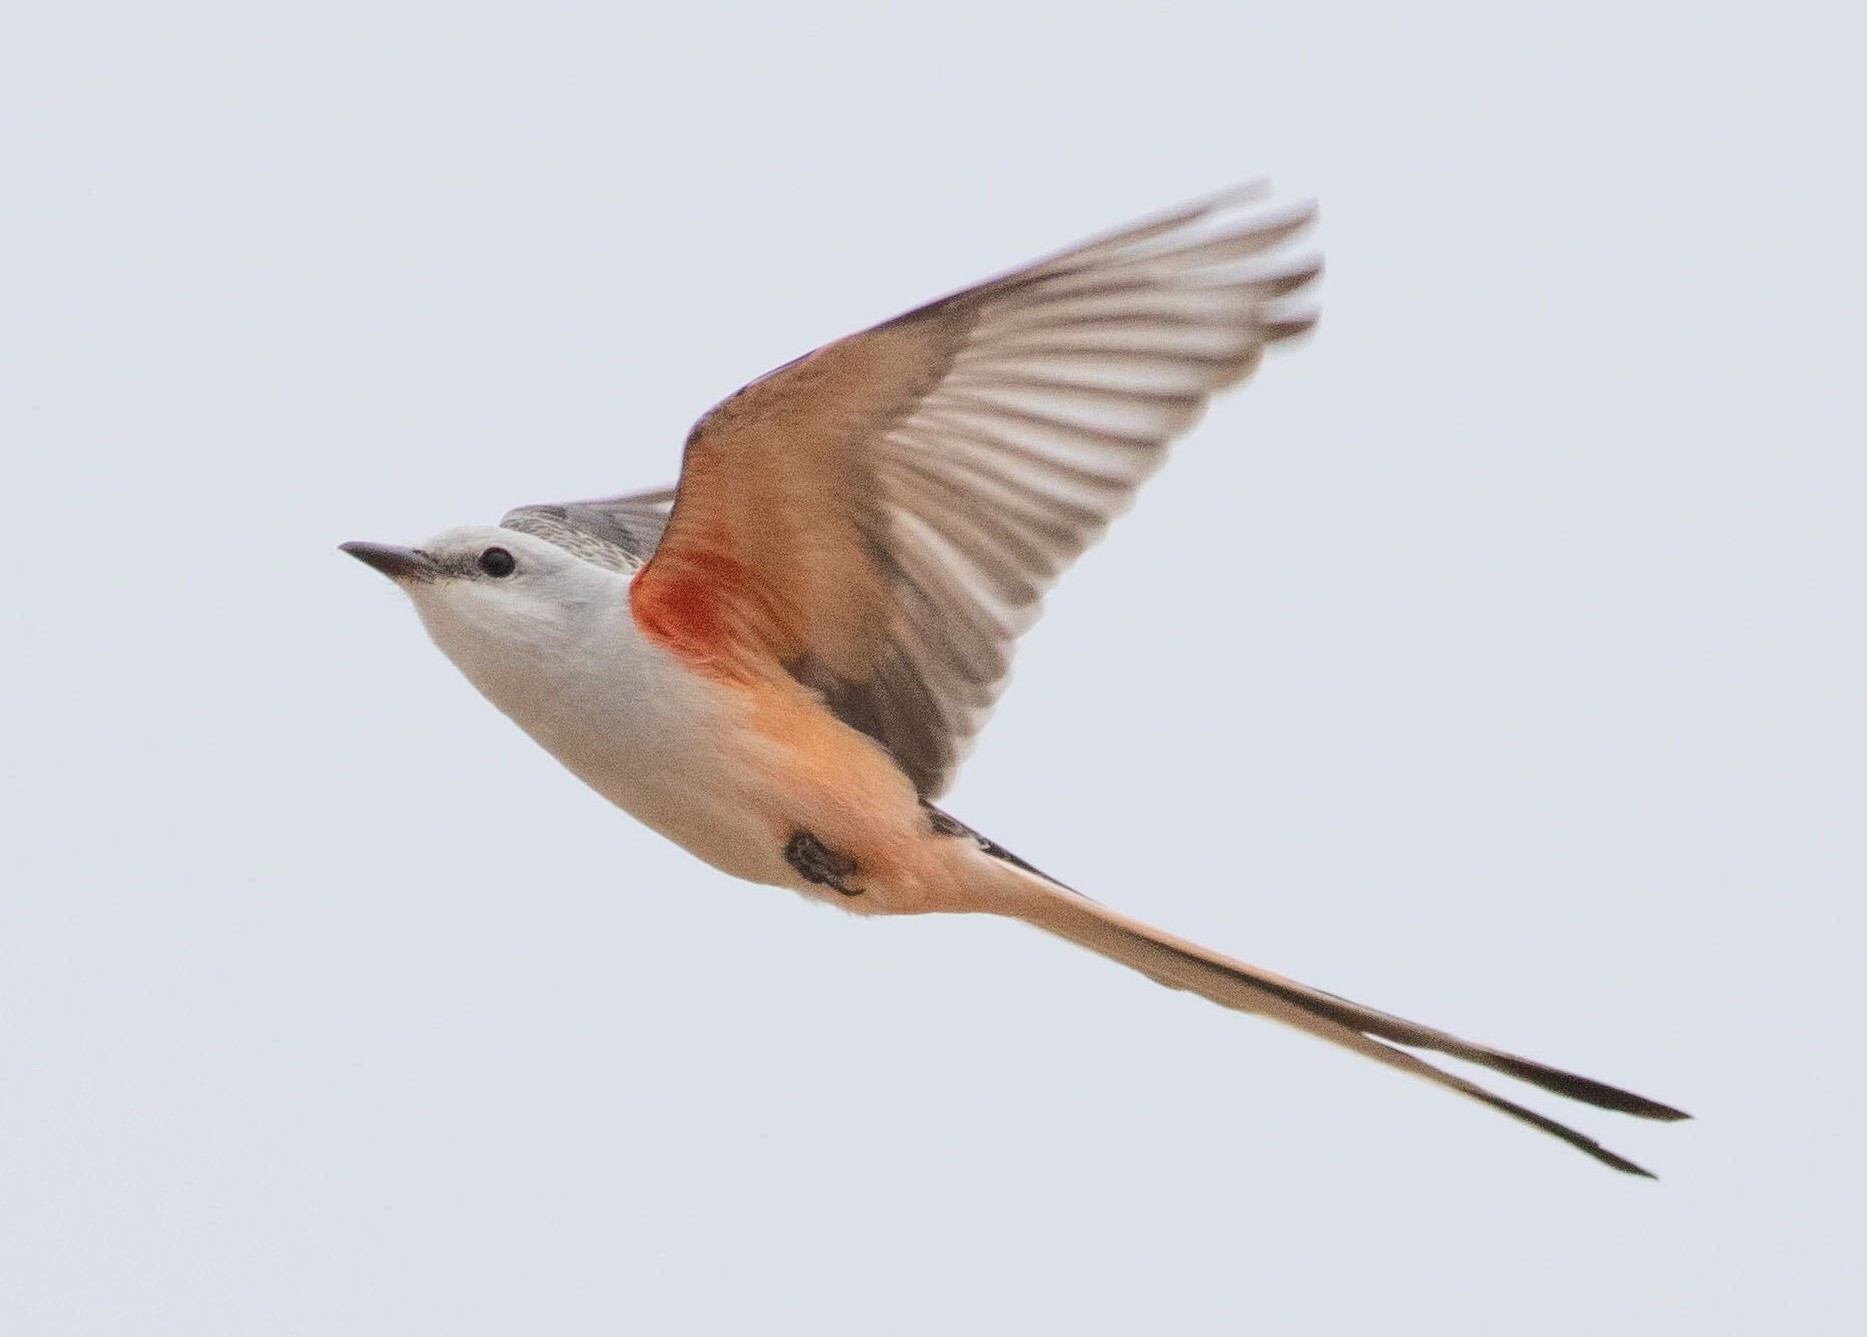
\includegraphics{./NickTepper-STFL.jpg}\\

\textbf{Suggested Citation}\\
Reese, J., McLaren, M. F., Smith, M., Walker, T., Timmer, J. M., White,
C. M., Pavlacky Jr., D. C., Sparks, R. A. 2023. Integrated Monitoring in
Bird Conservation Regions (IMBCR): 2022 Field Season Report. Bird
Conservancy of the Rockies. Brighton, Colorado, USA.

\textbf{Contact Information}\\
Matthew McLaren\\
matthew.mclaren@birdconservancy.org\\
970-482-1707

\end{footnotesize}}

Bird Conservancy of the Rockies (Bird Conservancy), in conjunction with
its partners, conducted the 15th consecutive year of landbird monitoring
for the Integrated Monitoring in Bird Conservation Regions (IMBCR)
program.

IMBCR is based on a spatially balanced sampling design which provides
inference to avian populations at various scales, from local management
units to entire states or Bird Conservation Regions, facilitating
conservation at local and national levels. The nested design also
provides a consistent and flexible framework for understanding and
comparing the status and annual changes of bird populations with local
and regional context.

Collaboration across organizations and spatial scales increases sample
sizes and improves the accuracy and precision of population estimates.
Analyzing the data collectively allows us to estimate detection
probabilities for species that would otherwise have insufficient numbers
of detections at local scales.

For these reasons, the IMBCR program is well-positioned to address
conservation and management needs for a wide range of stakeholders,
encouraging an interdisciplinary approach to bird conservation that
combines monitoring, research, and management.

\textbf{Bird Conservancy of the Rockies}\\
14500 Lark Bunting Lane\\
Brighton, CO 80603\\
303-659-4348\\
\href{https://birdconservancy.org}{www.birdconservancy.org}\\

\bookmarksetup{startatroot}

\hypertarget{about-us}{%
\chapter{About Us}\label{about-us}}

\marginnote{\begin{footnotesize}

\end{footnotesize}}

\hypertarget{connecting-people-birds-and-land}{%
\subsection*{Connecting people, birds and
land}\label{connecting-people-birds-and-land}}
\addcontentsline{toc}{subsection}{Connecting people, birds and land}

\textbf{Mission}: Conserving birds and their habitats through science,
education and land stewardship

\textbf{Vision}: Native bird populations are sustained in healthy
ecosystems

Bird Conservancy of the Rockies conserves birds and their habitats
through an integrated approach of science, education, and land
stewardship. Our work radiates from the Rockies to the Great Plains,
Mexico and beyond. Our mission is advanced through sound science,
achieved through empowering people, realized through stewardship, and
sustained through partnerships. Together, we are improving native bird
populations, the land, and the lives of people.

\begin{quote}
\textbf{Core Values}\\
1. Science provides the foundation for effective bird conservation.\\
2. Education is critical to the success of bird conservation.\\
3. Stewardship of birds and their habitats is a shared responsibility.
\end{quote}

\begin{quote}
\textbf{Goals}\\
1. Guide conservation action where it is needed most by conducting
scientifically rigorous monitoring and research on birds and their
habitats within the context of their full annual cycle.\\
2. Inspire conservation action in people by developing relationships
through community outreach and science-based, experiential education
programs.\\
3. Contribute to bird population viability and help sustain working
lands by partnering with landowners and managers to enhance wildlife
habitat.\\
4. Promote conservation and inform land management decisions by
disseminating scientific knowledge and developing tools and
recommendations.
\end{quote}

To learn more visit our website at
\href{https://birdconservancy.org}{www.birdconservancy.org}.

\bookmarksetup{startatroot}

\hypertarget{executive-summary}{%
\chapter{Executive Summary}\label{executive-summary}}

In 2022, the IMBCR program's area of inference encompassed four entire
states (Colorado, Montana, Utah, and Wyoming) and portions of 11
additional states (Arizona, California, Idaho, Kansas, Nebraska, Nevada,
New Mexico, North Dakota, Oklahoma, Oregon, and South Dakota). We
surveyed across US Forest Service (USFS) Regions 1, 2, and 4 and in
portions of Region 3; all of the Badlands and Prairies Bird Conservation
Region (BCR 17), and portions of nine other BCRs: Great Basin (9),
Northern Rockies (10), Prairie Potholes (11), Sierra Nevada (15),
Southern Rockies/Colorado Plateau (16), Shortgrass Prairie (18), Central
Mixed Grass Prairie (19), Sonoran and Mojave Deserts (33), and Sierra
Madre Occidental (34).

Observers conducted 15,066 point counts within 1,340 sampling units
between May 1 and July 25, 2022. They detected 194,859 individual birds
representing 355 species. This report summarizes the results of the 2022
field season.

\begin{quote}
To view interactive maps illustrating survey and detection locations,
and tables displaying species counts and population estimates (i.e.,
density and occupancy), please visit the
\href{http://rmbo.org/v3/avian/ExploretheData.aspx}{Rocky Mountain Avian
Data Center} (RMADC).
\end{quote}

\begin{tcolorbox}[enhanced jigsaw, breakable, colframe=quarto-callout-note-color-frame, toprule=.15mm, leftrule=.75mm, bottomrule=.15mm, rightrule=.15mm, left=2mm, arc=.35mm, colback=white, opacityback=0]

Instructions for using the RMADC are included in Appendix A of this
report and are available on the RMADC itself (hover over the ``Explore
the Data'' tab for tutorials). Each stratum or combination of strata
presented in this report's Results section contains a web link that
leads directly to the RMADC with the appropriate queries already
populated. Please note that not every stratum or conceivable combination
of strata is summarized in this report. However, all individual strata
and all biologically meaningful combinations of strata, or
``superstrata'', can be found on the RMADC.

\end{tcolorbox}

Long-term, rigorous monitoring provides valuable information on
population status, allowing managers and biologists to focus limited
resources on species of greatest concern. In the Discussion, we provide
a few examples demonstrating the use of IMBCR population trends for
tracking the status of designated species of concern and determining
where specific populations may require management or conservation
efforts.

\bookmarksetup{startatroot}

\hypertarget{tables-and-figures}{%
\chapter{Tables and Figures}\label{tables-and-figures}}

Table~{1} Planned and completed surveys by strata, 2022.

Table~{2} Reasons planned surveys were not completed, 2022.

Table~{3} Population trend estimates for sensitive sagebrush bird
species within select Wyoming Bureau of Land Management strata from the
IMBCR program.

Table~{4} Population trend estimates for two grassland bird species
within Bird Conservation Region 17 from the IMBCR program.

Table~{5} Population trend estimates for sensitive species within select
U.S. Forest Service National Grassland and National Forest strata from
the IMBCR program.

Table~{2} Reasons planned surveys were not completed, 2022.

\hypertarget{figures}{%
\section*{Figures}\label{figures}}
\addcontentsline{toc}{section}{Figures}

\markright{Figures}

\begin{tcolorbox}[enhanced jigsaw, breakable, colframe=quarto-callout-note-color-frame, toprule=.15mm, titlerule=0mm, leftrule=.75mm, toptitle=1mm, title=\textcolor{quarto-callout-note-color}{\faInfo}\hspace{0.5em}{Note}, opacityback=0, bottomtitle=1mm, coltitle=black, bottomrule=.15mm, colbacktitle=quarto-callout-note-color!10!white, left=2mm, arc=.35mm, rightrule=.15mm, colback=white, opacitybacktitle=0.6]

Figure numbers begin with their respective chapter numbers.

\end{tcolorbox}

Figure~\ref{fig-bcr-regions} Bird Conservation Regions throughout North
America, excluding Hawaii and Mexico.

Figure~\ref{fig-extent} Spatial extent of sampled Bird Conservation
Regions using the IMBCR design, 2022.

Figure~\ref{fig-sampling-unit} Example 1 km² sampling unit in the IMBCR
design.

Figure~\ref{fig-bcr-17} Survey locations and strata in Bird Conservation
Region 17, 2022

Figure~\ref{fig-co} Survey locations and strata in Colorado, 2022

Figure~\ref{fig-mt} Survey locations and strata in Montana, 2022.

Figure~\ref{fig-ut} Survey locations and strata in Utah, 2022.

Figure~\ref{fig-wy} Survey locations and strata in Wyoming, 2022.

\bookmarksetup{startatroot}

\hypertarget{introduction}{%
\chapter{Introduction}\label{introduction}}

Monitoring is an essential component of wildlife management and
conservation science (Marsh \& Trenham, 2008; Witmer, 2005). Common
goals of population monitoring are to estimate the population status of
target species and to detect changes in populations over time (Sauer \&
Knutson, 2008; Thompson, White, \& Gowan, 1998). In addition to
providing basic information on species distributions, effective
monitoring programs can identify species that are at-risk because of
small or declining populations (Dreitz, Lukacs, \& Knopf, 2006); provide
an understanding of how management actions affect populations
(Alexander, Stephens, Geupel, \& Will, 2008; Lyons, Runge, Laskowski, \&
Kendall, 2008); and evaluate population responses to landscape
alteration and climate change (Baron et al., 2008; Lindenmayer \&
Likens, 2009).

While monitoring at local scales remains critical, there is an
increasing need to monitor the consequences of environmental change over
large spatial and temporal scales and address questions much larger than
those that can be answered within individual management units (Dreitz,
Stinson, Hahn, Tack, \& Lukacs, 2017; Lindenmayer \& Likens, 2009).
Reconciling disparities between the geographic scale of management
actions and the scale of ecological and species-specific responses is a
persistent challenge for natural resource management agencies (Ruggiero,
Hayward, \& Squires, 1994). Population monitoring of eco-regional
landscapes provides an important context for evaluating population
change at local and regional scales, with the potential to identify
causal factors and management actions for species recovery (Manley,
Schlesinger, Roth, \& Van Horne, 2005; Sauer \& Knutson, 2008).

Before monitoring can be used by land managers to guide conservation
efforts, sound program designs and analytical methods are necessary to
produce unbiased population estimates (Sauer \& Knutson, 2008). At the
most fundamental level, reliable knowledge about the status of avian
populations requires accounting for spatial variation and incomplete
detection of the target species (Pollock et al., 2002; Rosenstock,
Anderson, Giesen, Leukering, \& Carter, 2002; Thompson, 2002).
Addressing spatial variation entails the use of probabilistic sampling
designs, which allows population estimates to be extended over the
entire area of interest (Thompson et al., 1998). Accounting for
incomplete detection involves the use of appropriate sampling and
analytical methods to address the fact that few, if any, species are so
conspicuous that they are detected with certainty when present during a
survey. Accounting for these two sources of variation ensures that
observed trends reflect true population changes rather than artifacts of
the sampling and observation processes (Pollock et al., 2002; Thompson,
2002).

The apparent large-scale declines of avian populations and the loss,
fragmentation and degradation of native habitats highlight the need for
extensive and rigorous landbird monitoring programs (Rich et al., 2004;
US North American Bird Conservation Initiative Monitoring Subcommittee,
2007). The US North American Bird Conservation Initiative's (NABCI)
``Opportunities for Improving Avian Monitoring'' (NABCI Monitoring
Subcommittee, 2007) provided goals for avian monitoring programs
including:

\begin{quote}
\textbf{Goal 1}: Fully integrate monitoring into bird management and
conservation practices and ensure that monitoring is aligned with
management and conservation priorities.

\textbf{Goal 2}: Coordinate monitoring programs among organizations and
integrate them across spatial scales to solve conservation or management
problems effectively.

\textbf{Goal 3}: Increase the value of monitoring information by
improving statistical design.

\textbf{Goal 4}: Maintain bird population monitoring data in modern data
management systems. Recognize legal, institutional, proprietary, and
other constraints while still providing greater availability of raw
data, associated metadata, and summary data for bird monitoring
programs.
\end{quote}

With the NABCI Monitoring Subcommittee (2007) guidelines in mind, Bird
Conservancy of the Rockies and partners initiated a broad-scale
collaborative bird monitoring program in 2008 entitled ``Integrated
Monitoring in Bird Conservation Regions'' (IMBCR) (Blakesley \& Hanni,
2009). See Appendix B: IMBCR Program and Stratification History for a
complete history of this program. The monitoring objectives of the IMBCR
partnership are to:

\begin{enumerate}
\def\labelenumi{\arabic{enumi}.}
\tightlist
\item
  Provide robust density, population and occupancy estimates that
  account for incomplete detection and are comparable at different
  geographic extents;
\item
  Provide long-term status and trend data for all regularly occurring
  breeding landbird species throughout the study area;
\item
  Provide a design framework to spatially integrate existing bird
  monitoring efforts in the region to provide better information on
  distribution and abundance of breeding landbirds, especially for high
  priority species;
\item
  Provide basic habitat association data for most bird species to
  address habitat management issues;
\item
  Maintain a high-quality database that effectively merges records
  between regional data nodes and is accessible to all of our
  collaborators as well as to the public over the internet, in the form
  of raw and summarized data; and
\item
  Generate decision support tools that help guide conservation efforts
  and provide a better measure of conservation success.
\end{enumerate}

The IMBCR design includes Bird Conservation Regions (BCRs) as sampling
frames (Figure~\ref{fig-bcr-regions}), stratified by land ownership
inside each BCR (NABCI Monitoring Subcommittee, 2007). BCRs provide a
spatially consistent framework for bird conservation in North America.
Each BCR represents a distinct ecological region with similar bird
communities, vegetation types, and resource management interests (NABCI,
2000). Population monitoring within BCRs is implemented with a flexible
hierarchical framework of nested units, where information on bird
populations can be partitioned into smaller units for small-scale
conservation planning, or aggregated to support large-scale conservation
efforts. By focusing on scales relevant to management and conservation,
information obtained from monitoring in BCRs can be integrated into
research and management objectives at various scales applicable to
managers (Pavlacky et al., 2017; Ruth et al., 2003).

\begin{figure}

{\centering 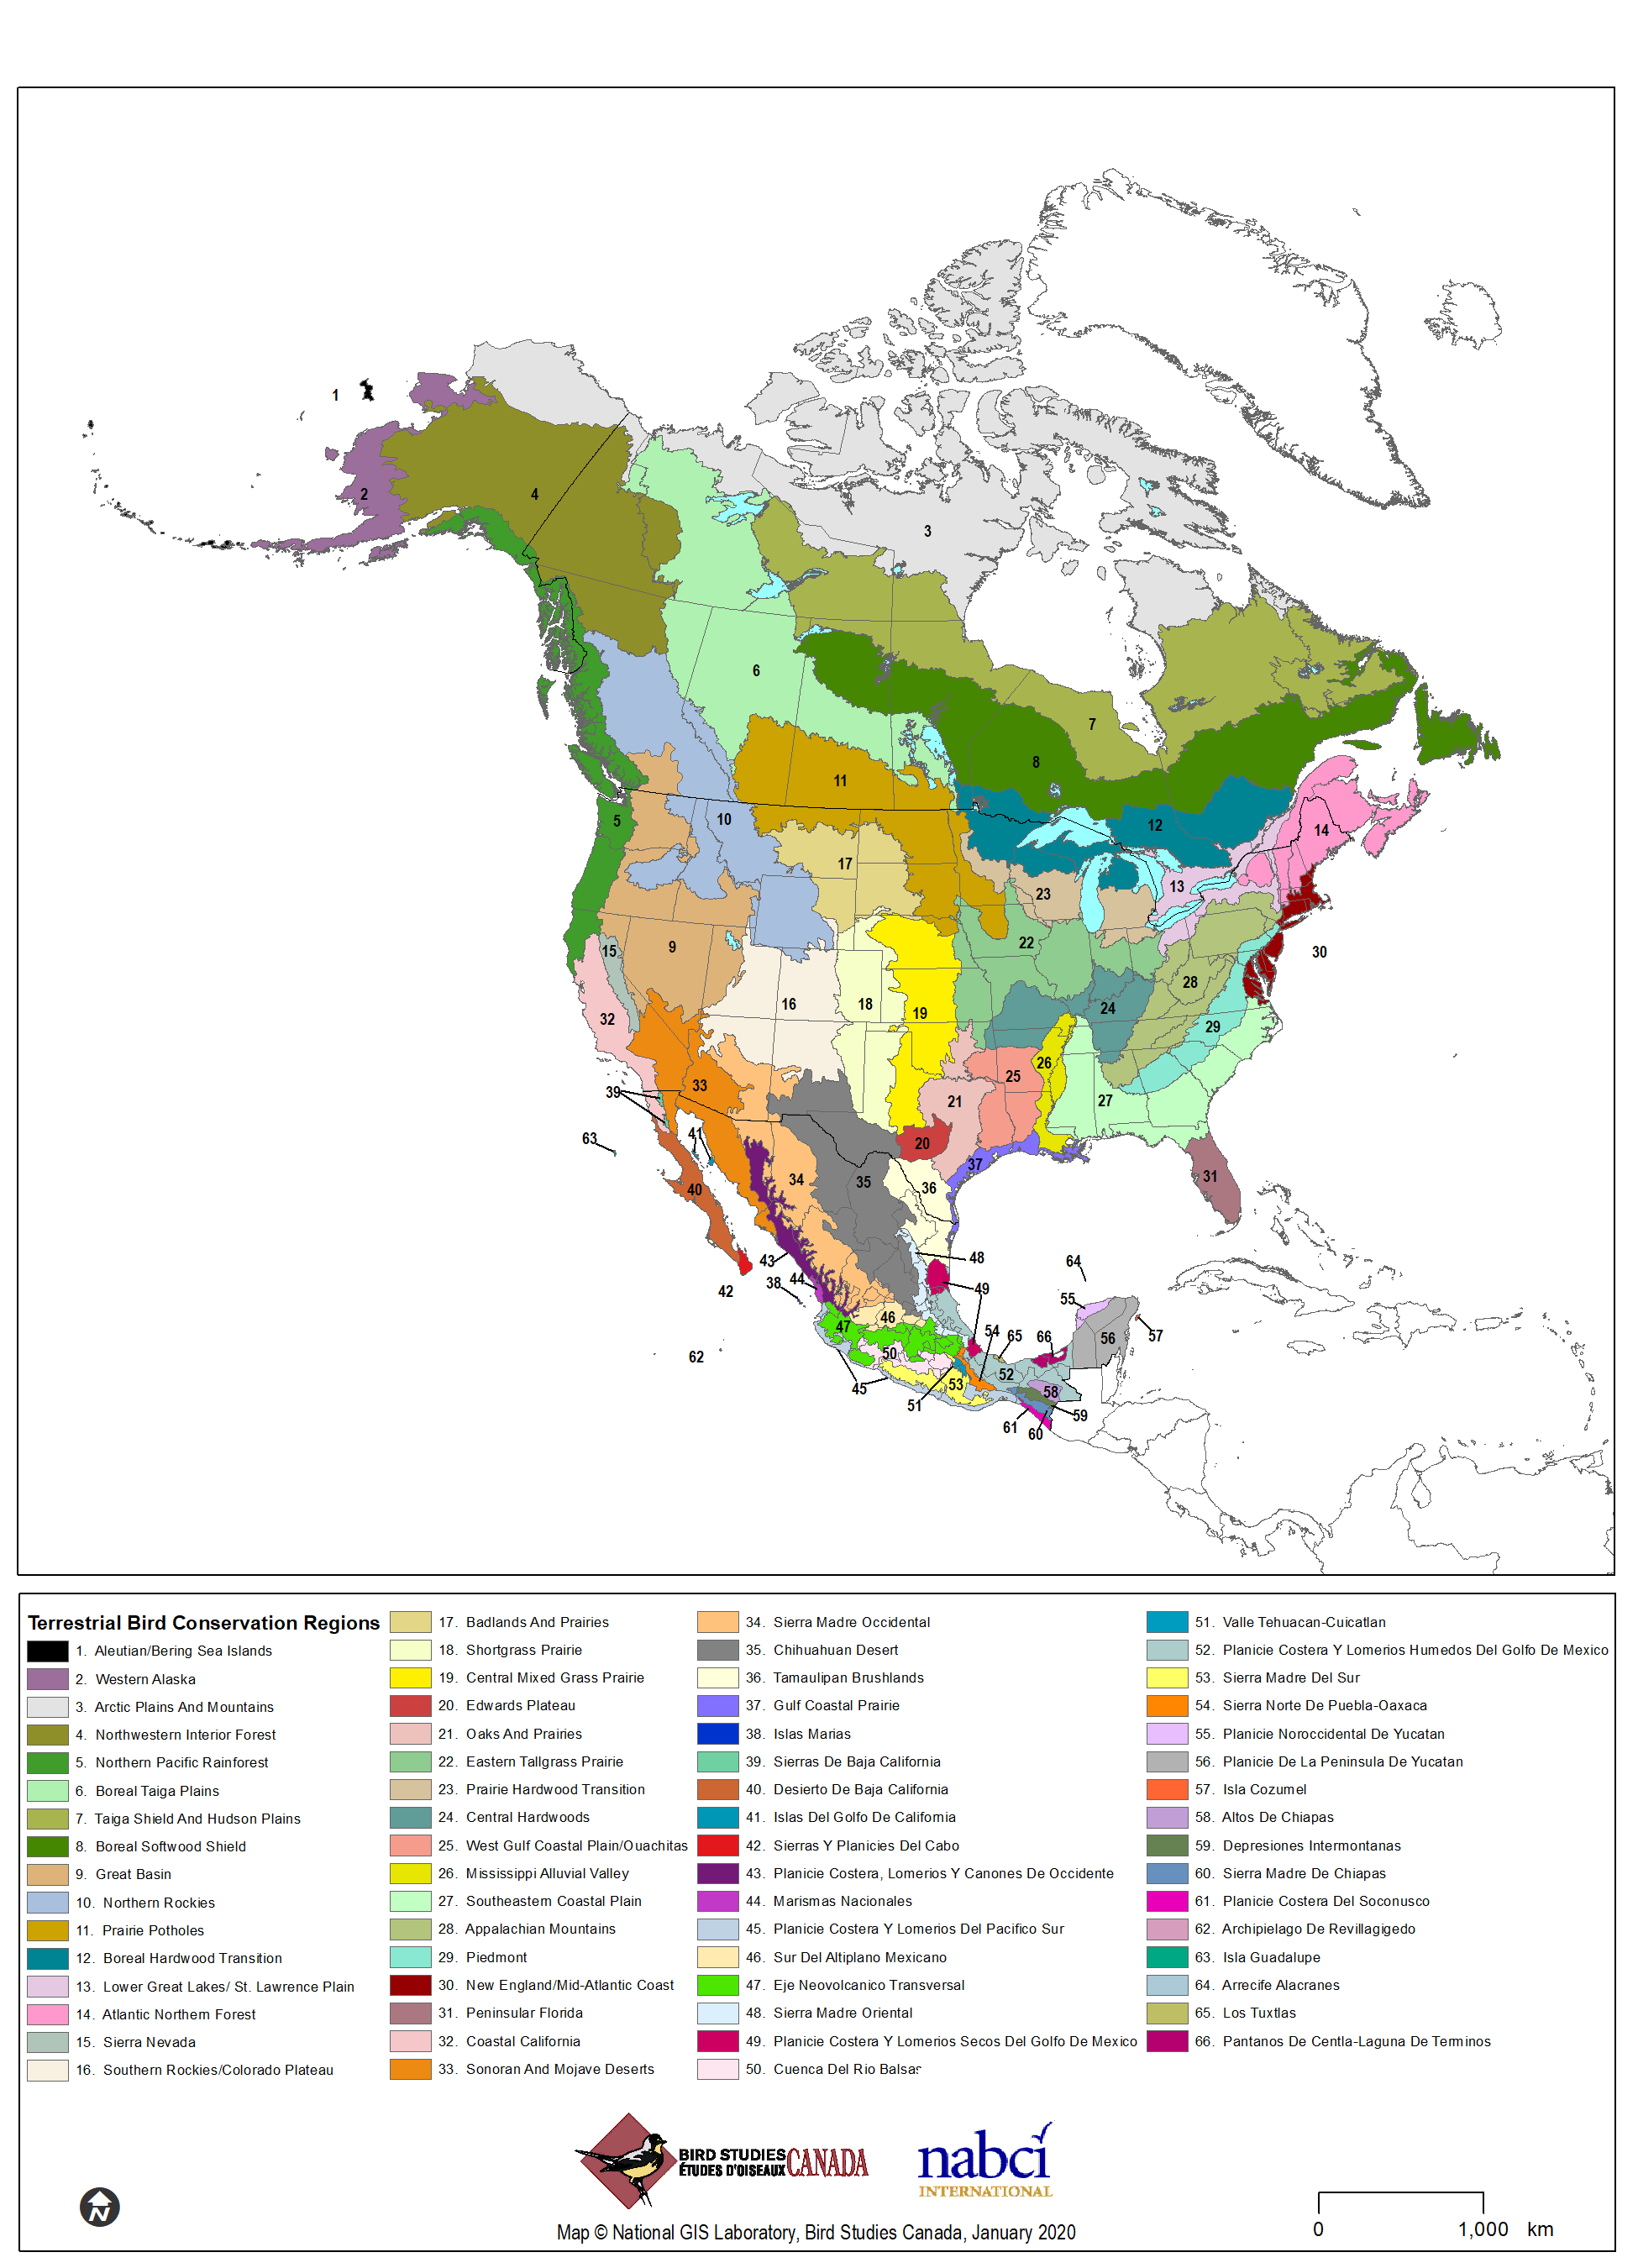
\includegraphics{./BCR_Terrestrial.png}

}

\caption{\label{fig-bcr-regions}Bird Conservation Regions throughout
North America, excluding Hawaii and Mexico}

\end{figure}

\bookmarksetup{startatroot}

\hypertarget{methods}{%
\chapter{Methods}\label{methods}}

\hypertarget{study-area}{%
\section{Study Area}\label{study-area}}

In 2022, the IMBCR program's area of inference encompassed four entire
states (Colorado, Montana, Utah, and Wyoming) and portions of 11
additional states (Arizona, California, Idaho, Kansas, Nebraska, Nevada,
New Mexico, North Dakota, Oklahoma, Oregon, and South Dakota). We
surveyed across US Forest Service (USFS) Regions 1, 2, and 4 and in
portions of Region 3; all of the Badlands and Prairies Bird Conservation
Region (BCR 17), and portions of nine other BCRs: Great Basin (9),
Northern Rockies (10), Prairie Potholes (11), Sierra Nevada (15),
Southern Rockies/Colorado Plateau (16), Shortgrass Prairie (18), Central
Mixed Grass Prairie (19), Sonoran and Mojave Deserts (33), and Sierra
Madre Occidental (34).

\begin{figure}

{\centering 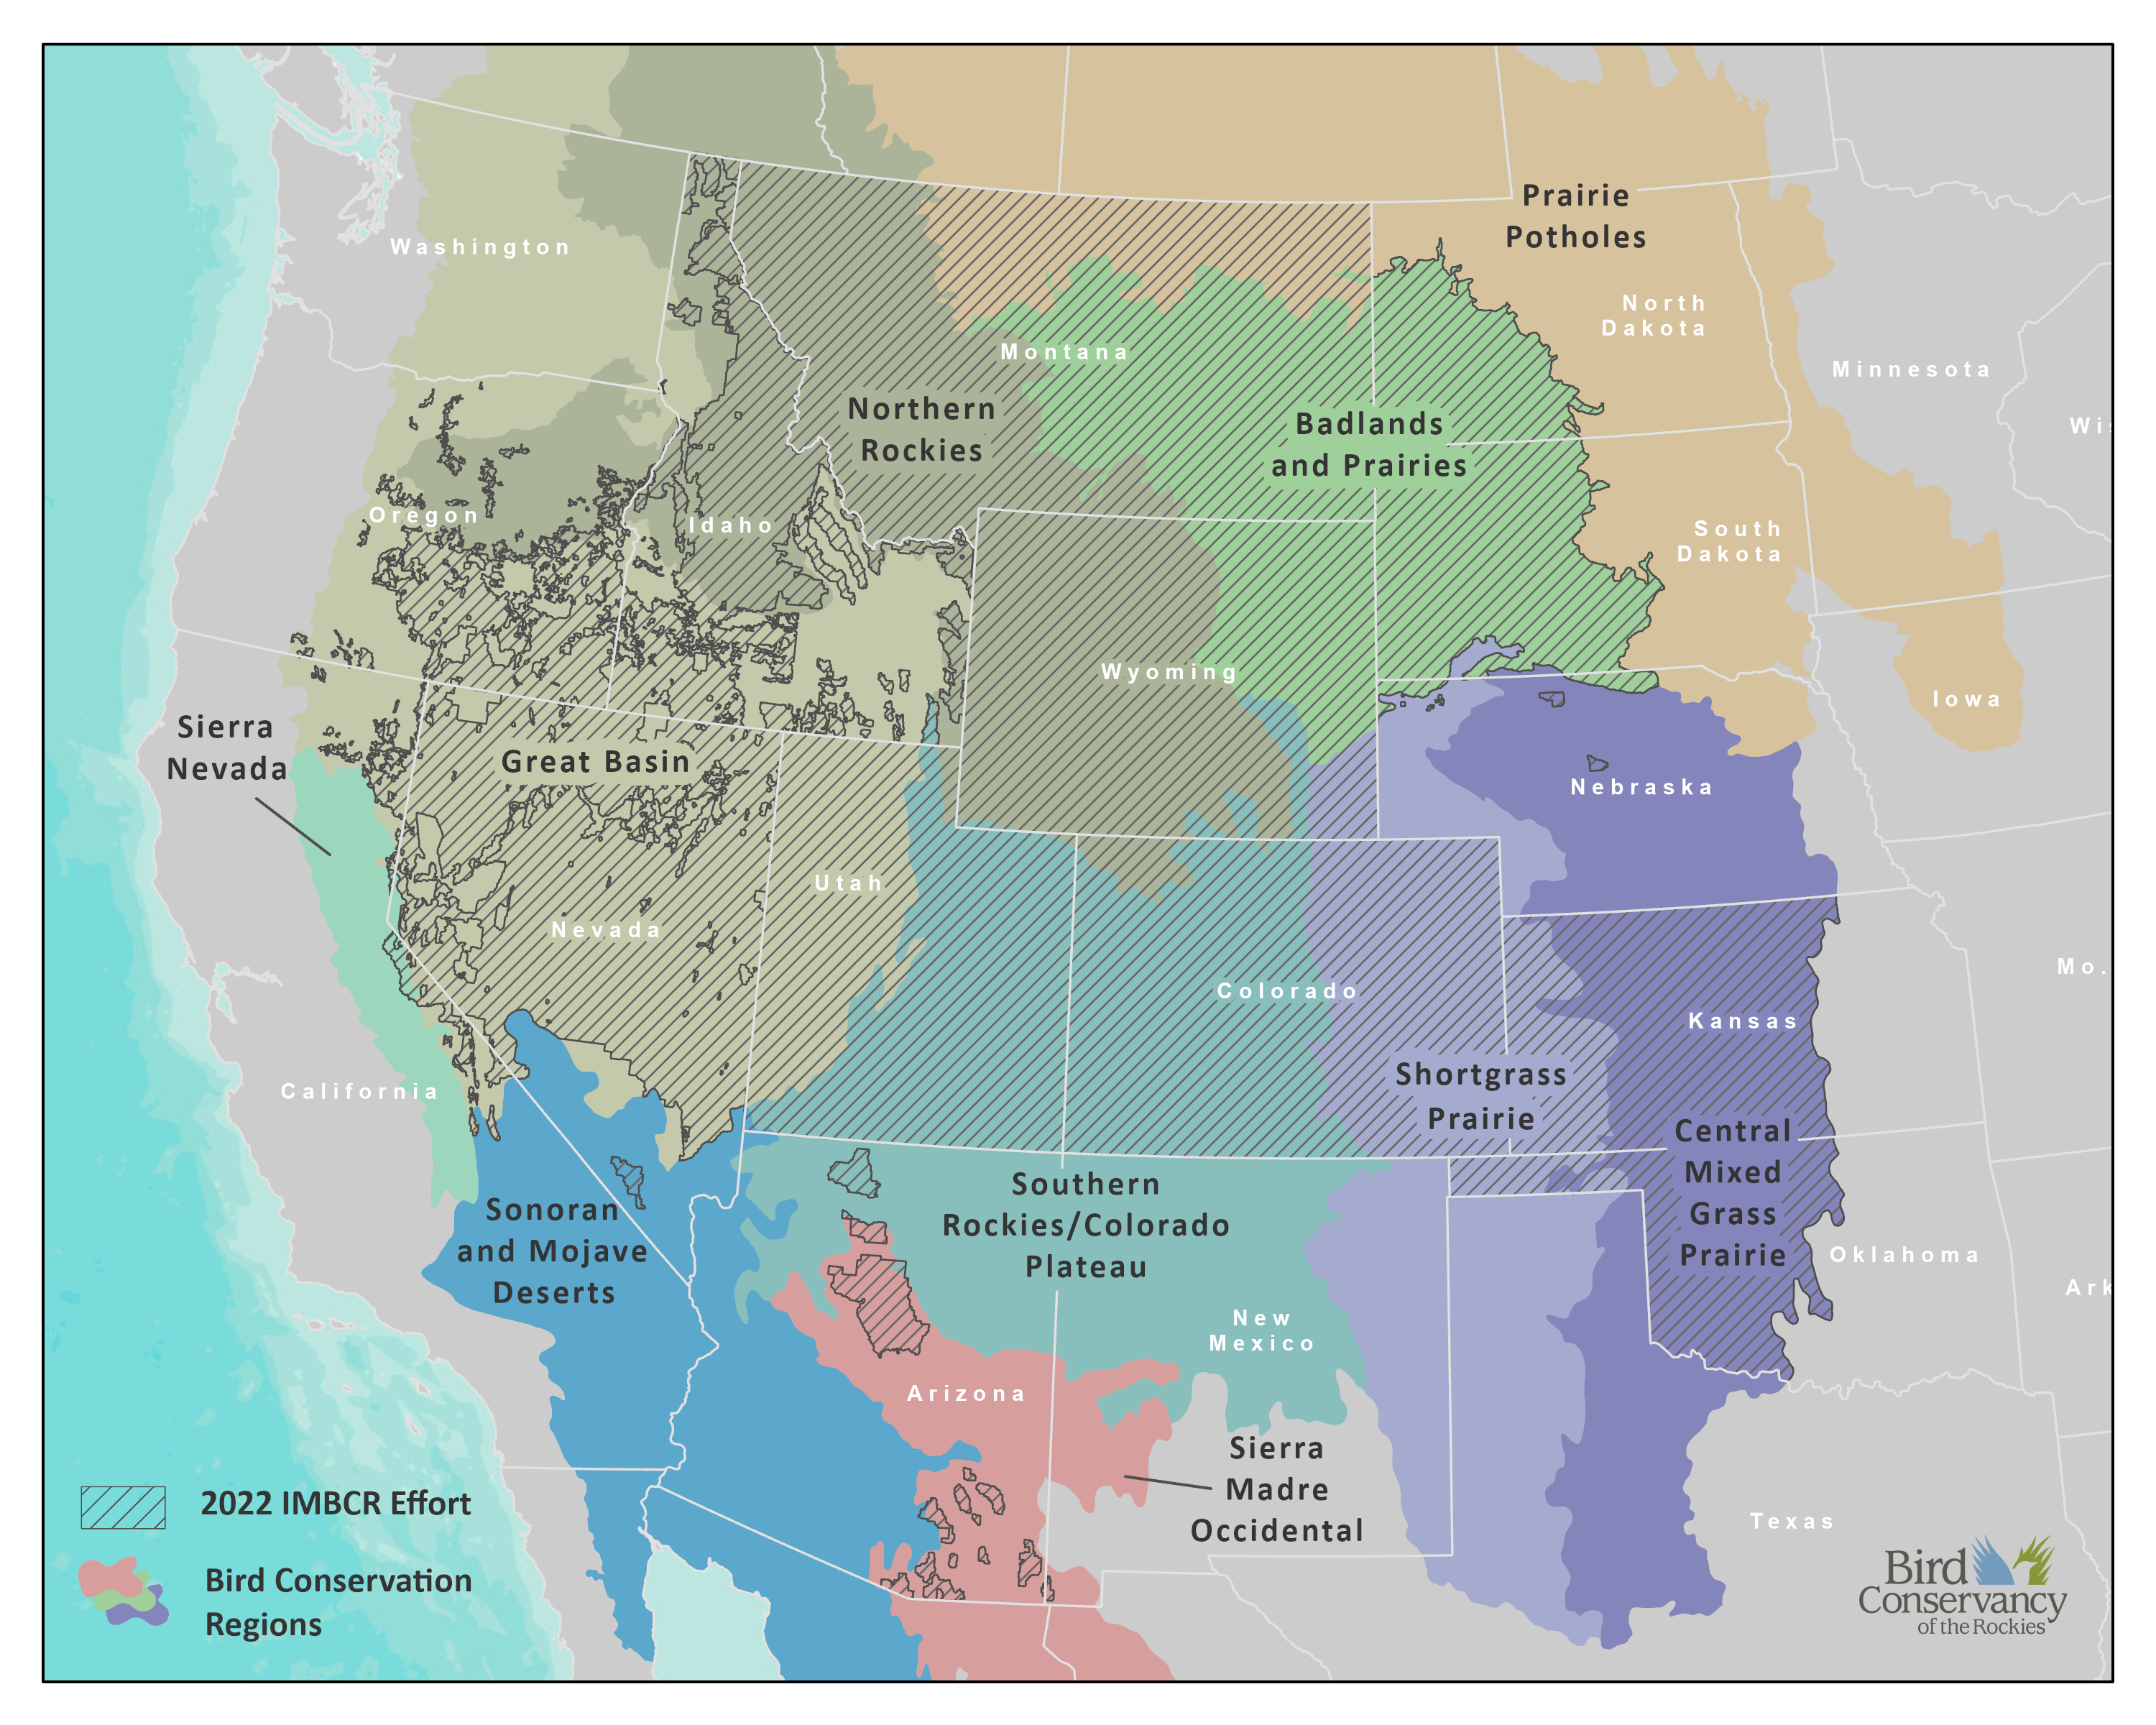
\includegraphics{./IMBCR_Extent_Map_2022.png}

}

\caption{\label{fig-extent}Spatial extent of sampled Bird Conservation
Regions using the IMBCR design, 2022}

\end{figure}

\hypertarget{sampling-design}{%
\section{Sampling Design}\label{sampling-design}}

\hypertarget{sampling-frame-and-stratification}{%
\subsection{Sampling Frame and
Stratification}\label{sampling-frame-and-stratification}}

A key component of the IMBCR design is the ability to infer about bird
populations across spatial scales, from small management units, such as
individual national forests or field offices, to entire states and BCRs.
This is accomplished through hierarchical (nested) stratification, which
allows data from smaller-order strata to be combined to make inferences
about higher-order strata. For example, data from each individual
national forest stratum in USFS Region 2 are combined to produce
Region-wide population estimates; data from each individual stratum in
Montana are combined to produce statewide estimates; and data from each
individual stratum in BCR 17 are combined to produce BCR-wide estimates.

We define strata based on areas to which IMBCR partners wanted to make
inferences. We defined the largest sampling frame as the intersection of
state and BCR boundaries (e.g., Wyoming-BCR 10). We base the strata
within the state-BCR sampling frames on fixed attributes, such as land
ownership boundaries, elevation zones, major river systems and
wilderness/roadless designations.

\hypertarget{sampling-units}{%
\subsection{Sampling Units}\label{sampling-units}}

We define sampling units as 1 km² cells, each containing 16 evenly
spaced sample points, 250 meters apart (Figure 3). We define potential
sampling units by superimposing a uniform grid of cells over each state
in the study area. We then assign each cell to a stratum using ArcGIS
version 10.X and higher (Environmental Systems Research Institute,
2017). For all stratifications developed after 2012, we use the United
States National Grid (USNG), a nonproprietary alphanumeric referencing
system derived from the Military Grid Reference System that was created
by the Federal Geographic Data Committee.

\begin{figure}

{\centering 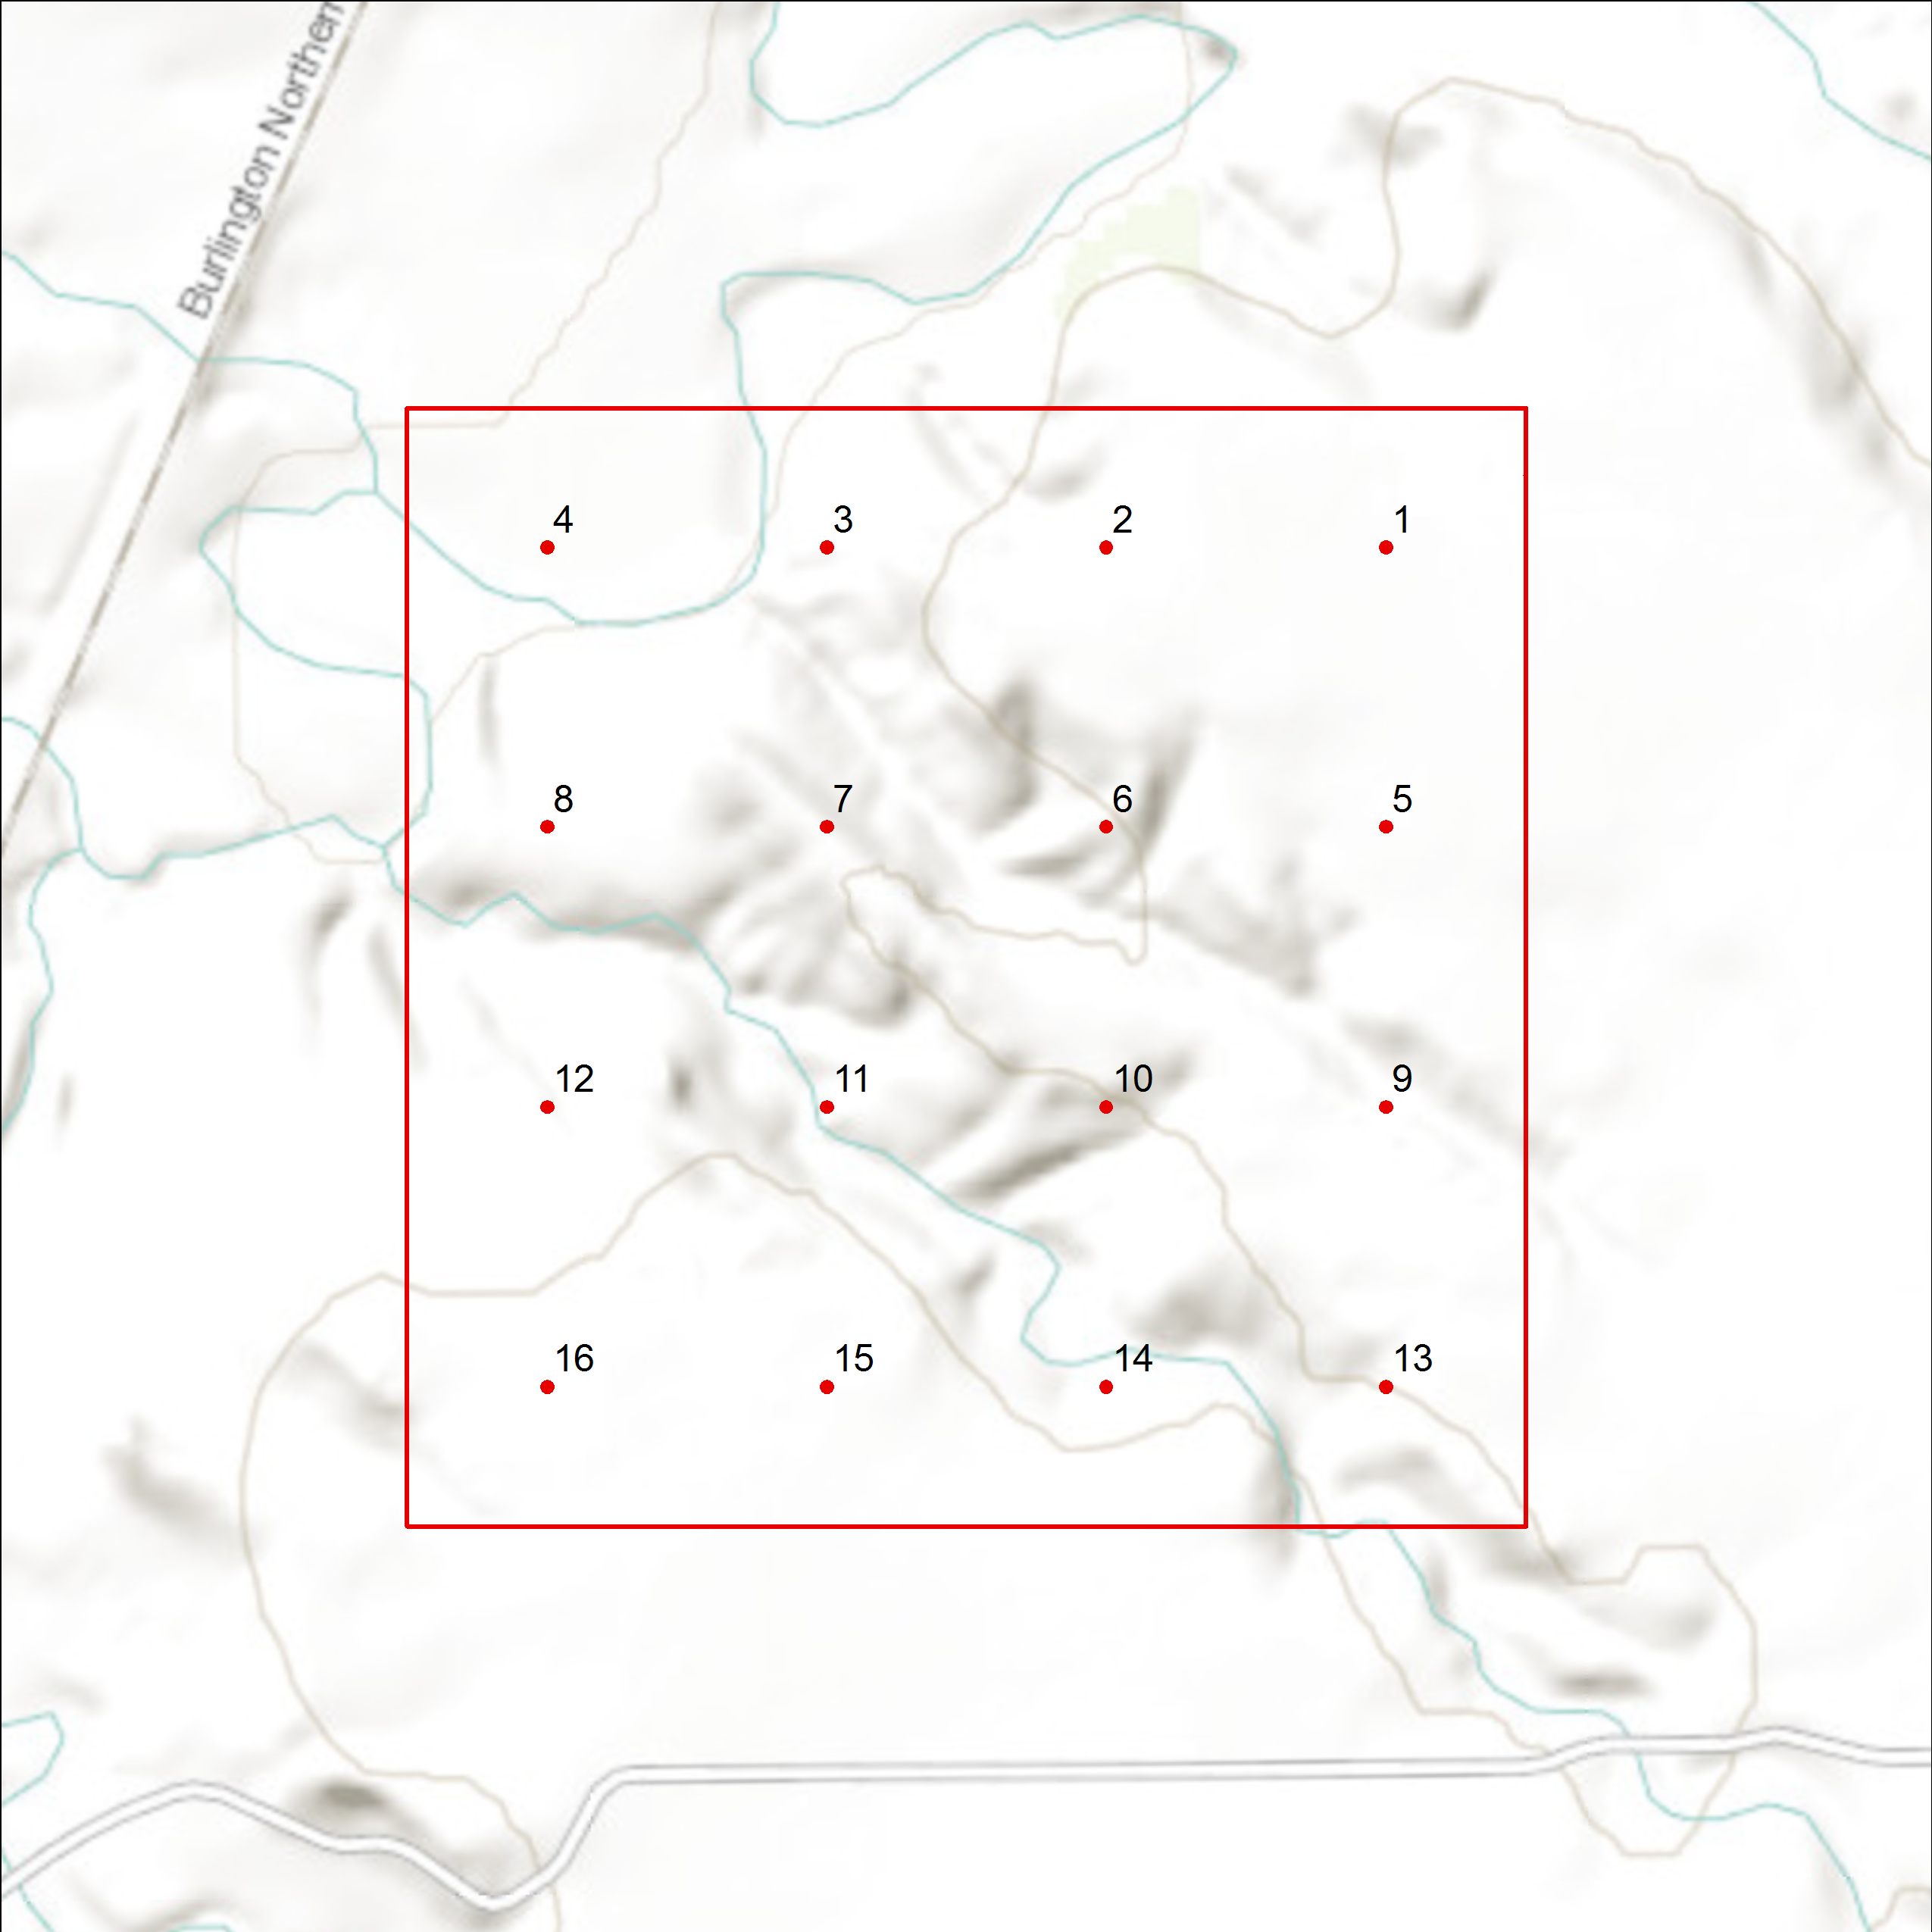
\includegraphics[width=0.5\textwidth,height=\textheight]{./IMBCR-sampling-unit.png}

}

\caption{\label{fig-sampling-unit}Example 1 km² sampling unit in the
IMBCR design.}

\end{figure}

\hypertarget{sample-selection}{%
\subsection{Sample Selection}\label{sample-selection}}

Within each stratum, we use generalized random-tessellation
stratification (GRTS), a spatially balanced sampling algorithm, to
select sampling units (Stevens Jr.~\& Olsen, 2004). The GRTS design has
useful properties with respect to long-term monitoring of birds at large
spatial scales including:

\begin{itemize}
\item
  Spatially balanced sampling is generally more efficient than simple
  random sampling of natural resources (Stevens Jr.~\& Olsen, 2004).
  Incorporating information about spatial autocorrelation in the data
  can increase precision in density estimates.
\item
  All sampling units in the sampling frame are ordered, such that any
  set of consecutively numbered units is a spatially well-balanced
  sample (Stevens Jr.~\& Olsen, 2004). In the case of fluctuating
  budgets, IMBCR partners can adjust the sampling effort among years
  within each stratum while still preserving a random, spatially
  balanced sampling design.
\end{itemize}

A minimum of two sampling units within each stratum are required to
estimate the variances of population parameters. However, reliable
stratum-level occupancy estimates require larger sample sizes, with a
minimum of approximately 8-10 samples per stratum. Additional samples
may be required for strata comprising large geographic areas. Because we
estimate regional density and occupancy using an area weighted mean,
adding more samples to a particular stratum does not bias the overall
estimate, it simply increases the precision. After the initial two
sampling units were selected, the remaining allocation of sampling
effort among strata was based on the priorities of the funding partners.

\hypertarget{sampling-methods}{%
\section{Sampling Methods}\label{sampling-methods}}

IMBCR observers with excellent aural and visual bird-identification
skills conducted field work in 2020. Prior to conducting surveys,
observers completed an intensive training program that was largely
virtual to ensure full understanding of the field protocol and review
bird and plant identification. Observers were also shadowed by a crew
leader at the start of the field season to ensure they understood the
protocol and could identify all birds within a region.

Observers conducted point counts (Buckland et al., 2001) following
protocols established by IMBCR partners (Hanni, White, Birek, Van Lanen,
\& McLaren, 2012). Observers conducted surveys in the morning, beginning
one-half hour before sunrise and concluding no later than five hours
after sunrise. Observers recorded the start time for every point count
conducted. For every bird detected during the six-minute period,
observers recorded species, sex, horizontal distance from the observer,
minute, type of detection (e.g., call, song, visual), whether the bird
was thought to be a migrant, and whether the observer was able to
visually identify each record.

Observers measured distances to each bird using laser rangefinders when
possible. When it was not possible, observers estimated the distance by
measuring to some object near the bird using a laser rangefinder. In
addition to recording all bird species detected in the area during point
counts, observers recorded birds flying over but not using the immediate
surrounding landscape. Observers also recorded Abert's squirrel (Sciurus
aberti), American red squirrel (Tamiasciurus hudsonicus), and American
pika (Ochotona princeps). While observers traveled between points within
a sampling unit, they recorded the presence of any species not recorded
during a point count. The opportunistic detections of these species are
used for distribution purposes only.

Observers considered all non-independent detections of birds (i.e.,
flocks or pairs of conspecific birds together in close proximity) as
part of a ``cluster'' rather than as independent observations. Observers
recorded the number of birds detected within each cluster along with a
letter code to distinguish between multiple clusters.

At the start and end of each survey, observers recorded time, ambient
temperature, cloud cover, precipitation, and wind speed. Observers
navigated to each point using hand-held Global Positioning System units.
Before beginning each six-minute count, surveyors recorded vegetation
data within a 50m radius of the point via ocular estimation. Vegetation
data included the dominant habitat type and relative abundance, percent
cover and mean height of trees and shrubs by species, grass height, and
ground cover. Observers recorded vegetation data quietly to allow birds
time to return to their normal habits prior to beginning each count.

For more detailed information about survey methods and vegetation data
collection protocols, refer to Bird Conservancy's Field Protocol for
Spatially Balanced Sampling of Landbird Populations on our
\href{http://rmbo.org/v3/avian/DataCollection.aspx}{Avian Data Center}.
You will also find links to past and current protocols and data sheets.

\hypertarget{data-analysis}{%
\section{Data Analysis}\label{data-analysis}}

\hypertarget{distance-analysis-assumptions}{%
\subsection{Distance Analysis
Assumptions}\label{distance-analysis-assumptions}}

Distance sampling theory was developed to account for the decreasing
probability of detecting an object of interest (e.g., a bird) with
increasing distance from the observer to the object (Buckland et al.,
2001). The detection probability is used to adjust the count of birds to
account for birds that were present but undetected. Application of
distance theory requires that five critical assumptions be met: 1) all
birds at and near the sampling location (distance = 0) are detected; 2)
distances to birds are measured accurately; 3) birds do not move in
response to the observer's presence (Buckland et al., 2001; Thomas et
al., 2010); 4) cluster sizes are recorded without error; and 5) the
sampling units are representative of the entire survey region (Buckland,
Marsden, \& Green, 2008).

\hypertarget{density-estimation}{%
\subsection{Density Estimation}\label{density-estimation}}

We developed a Bayesian, zero-inflated N-mixture model (Royle 2004,
Sillett et al.~2011) to estimate density and abundance for all strata
and superstrata across all species with sufficient data. We used
distance sampling to estimate detection probabilities and adjust counts
accordingly. For a detailed description of statistical analyses
performed, see (Appendix D).

Bayesian approaches to density estimation provide several benefits over
traditional distance sampling analyses, while providing similar and
unbiased estimates of density and abundance. First, with the nested
design of IMBCR, point count locations within a 1-km2 grid cell are not
independent. Therefore, with traditional methods, it is necessary to
treat each point as a spatial replicate within the grid cell(i.e.,
average counts across points). However, it is unlikely that bird
densities are uniform within a grid cell, and a better solution would be
to estimate density at the point count location. Bayesian models provide
the flexibility to do this, while correctly accounting for the lack of
independence among points. The second benefit, also provided by this
flexibility, is the ability to include covariates to explain changes in
density. This allows us to explicitly estimate the response of bird
density to variables, such as habitat variables, management actions, or
time (i.e., trend). Finally, Bayesian approaches allow for sharing of
information across parameters. This can assist in obtaining estimates at
sites with little data or provide measures of uncertainty when no birds
were detected, such as at low densities and/or small sample sizes.

We fit a series of models to the data from each species that had the
same model structure describing density estimation but varied in
detection structure (see Observation process section below). We used
zero-inflation to account for excess zeros in the data, where abundance
at a point count location (N) is conditional on the point's true
occupancy state (z) of a species at the point count location, and the
mean abundance within a 1-km2 grid cell was modeled as a function of
year to estimate stratum-specific trends.

All points within a grid cell shared a mean abundance to account for the
lack of independence of those points, but abundance was allowed to vary
spatially within a grid cell (i.e., by point) through Poisson variation.
To avoid predicting species occurrence outside of observed ranges, we
fixed occupancy probabilities to 0 for all strata in which the species
was never observed and used a prior informed by the observed proportion
of grid-year combinations in a stratum in which the species was
detected.

We derived density at the point count location by dividing the estimated
abundance by the area of the point count circle (see Observation process
section below) and multiplying by cluster size. We derived stratum-level
density estimates by averaging all point-level density estimates within
each stratum, and we took the area-weighted average of strata estimates
to obtain superstratum estimates.

\textbf{Observation process}

We estimated the probability of detecting an independent cluster of
individuals by fitting distance functions to the distance data collected
during surveys (Buckland et al.~2001). We fit four detection models
including:\\
1. half-normal constant (HN(.))\\
2. hazard rate constant (Haz(.))\\
3. half-normal year (HN(t))\\
4. hazard rate year (Haz(t))

We removed the furthest 10\% of observed detection distances from the
data set and binned the remaining detections into 10 evenly spaced
distance classes. The furthest remaining detection distance became the
radius of the point count circle with which we estimated density.

\textbf{Detection model selection}

To minimize computing time but find the most parsimonious detection
function, we fit detection-only models to the distance data, using the
four model structures described above. We used the Watanabe-Akaike
Information Criterion (WAIC; Watanabe 2010, Hooten and Hobbs 2015) to
select the most parsimonious detection structure and then used that
structure for detection probabilities in the full model to estimate
density and abundance.

\textbf{Trend Estimates}

We estimated trends for individual strata by calculating the
least-squares regression mean and standard errors for the intercept and
slope of the log densities across the monitoring period. We calculated
these parameters for every Bayesian iteration to account for uncertainty
around density estimates.

We developed a post-hoc approach to estimate trends for superstrata.
Using the rolled-up estimates of density for a superstratum, we fit a
general linear model (GLM) to the samples from each Bayesian iteration.
Fitting a GLM across iterations allowed us to incorporate uncertainty in
superstratum trends due to uncertainty around density estimates, but it
did not account for temporal variation. To incorporate this second form
of variation, we sampled a random intercept and slope for each iteration
using the mean and standard error estimated using the GLM and made
inference on the distribution of the resampled values.

\hypertarget{occupancy-analysis}{%
\subsection{Occupancy Analysis}\label{occupancy-analysis}}

Occupancy estimation is most commonly used to quantify the proportion of
sample units (i.e., 1 km² cells) occupied by an organism (MacKenzie et
al., 2002). The application of occupancy modeling requires multiple
surveys of the sample unit in space or time to estimate a detection
probability (MacKenzie et al., 2006). The detection probability adjusts
the proportion of sites occupied to account for species that were
present but undetected (MacKenzie et al., 2002). We used a removal
design (MacKenzie et al., 2006), to estimate a detection probability for
each species, in which we binned minutes one and two, minutes three and
four and minutes five and six to meet the assumption of a monotonic
decline in the detection rates through time. After the target species
was detected at a point, we set all subsequent sampling intervals at
that point to ``missing data'' (MacKenzie et al., 2006).

The 16 points in each sampling unit served as spatial replicates for
estimating the proportion of points occupied within the sampled sampling
units. We used a Bayesian, multi-scale occupancy model (Nichols et
al.~2008, Mordecai et al.~2011, Green et al.~2019) to estimate 1) the
probability of detecting a species given presence (p), 2) the proportion
of points occupied by a species given presence within sampled sampling
units (θ, Theta) and 3) the proportion of sampling units occupied by a
species (ψ, Psi).

We truncated the data, using only detections \textless125 m from the
sample points, except for Accipitriformes, Anseriformes, Falconiformes,
Galliformes, Gruiformes, Pelecaniformes, Podicepidiformes, and
Suliformes for which we used the maximum observed distance for each
species. Truncating the data allowed us to use bird detections over a
consistent plot size and ensured that the points were independent
(points were spread 250 m apart), which in turn allowed us to estimate θ
(the proportion of points occupied within each sampling unit) (Pavlacky
Jr., Blakesley, White, Hanni, \& Lukacs, 2012). The interpretation of θ
for species for which we used maximum distances changes from occupancy
to use because point count buffers overlap, but we chose this approach
to provide estimates for a larger number of species.

We expected regional differences in the behavior, habitat use, and local
abundance of species would correspond to regional variation in detection
and the fraction of occupied points. Therefore, we estimated the
proportion of sampling units occupied (ψ) for each stratum by estimating
BCR-by-year specific estimates of detection (p) and point-level
occupancy (θ). We fixed p and θ to 0 for BCRs in which a particular
species was never detected.

We fixed ψ to 0 for all strata in which the species was never detected.
As with density, we took an area-weighted mean of stratum-level
occupancy estimates (i.e.,ψ) to estimate superstratum-level occupancy
probabilities. The true point-level occupancy state was conditional on
the grid-cell-level occupancy state (i.e., occupied or unoccupied), such
that a point could only be occupied if the grid cell was occupied.
Finally, we modeled the observation process conditional on the point
being occupied using removal modeling.

Our application of the multi-scale model was analogous to a
within-season robust design (Pollock, 1982) where the two-minute
intervals at each point were the secondary samples for estimating p and
the points were the primary samples for estimating θ (Nichols et al.,
2008; Pavlacky Jr.~et al., 2012). We considered both p and θ to be
nuisance variables that were important for generating unbiased estimates
of ψ. θ can be considered an availability parameter or the probability a
species was present and available for sampling at the points (Nichols et
al., 2008; Pavlacky Jr.~et al., 2012).

\hypertarget{automated-analysis}{%
\subsection{Automated Analysis}\label{automated-analysis}}

In 2019, we updated our analytical methods to use Bayesian hierarchical
models specifically designed for analysis of IMBCR data. We performed
all data and output manipulation in R (R Core Team, 2022) and model
fitting in JAGS (Plummer 2003, 2017) using the R package jagsUI (Kellner
2018). The R code called the raw data from the IMBCR Structured Query
Language (SQL) server database and reformatted the data into a form
usable with the JAGS code. We allowed the input of all data collected in
a manner consistent with the IMBCR design to increase the number of
detections available for estimating global detection rates for
population density and site occupancy. The R code provided an automated
framework for combining stratum-level estimates of population density
and site occupancy at multiple spatial scales, as well as estimating the
standard deviations and credible intervals for the combined estimates.

We fit initial models to all species with at least 30 detections for
density estimation and 10 detections for occupancy estimation. For
density estimation, we fit the full model after determining whether
there were enough detections based on results from the detection-only
model fits. In some cases for both density and occupancy estimation, it
was necessary to use a less parsimonious detection structure or
simplified model structure to facilitate model convergence. We currently
maintain version control of the automated analysis code in the Bird
Conservancy repository on www.github.com.

\part{Results}

\hypertarget{summary}{%
\chapter{Summary}\label{summary}}

In 2022, field observers completed 1,348 of 1,415 (95.2\%) planned
surveys throughout all or portions of BCRs 9, 10, 11, 15, 16, 17, 18,
19, 33, and 34 using the IMBCR design ( Table~{1},
Figure~\ref{fig-extent}). Five surveys were completed above the funded
sample effort in two strata. Reasons surveys were not completed are
summarized in Table~{2}.

Observers conducted 15,137 point counts within the 1,348 surveyed
sampling units between May 1 and July 25, 2022. They detected 176,954
individual birds representing 350 species.

Please note that not every stratum or superstratum is summarized in this
report. We include details of specific strata or superstrata for which
our partners are most interested. However, results from all strata and
all biologically meaningful superstrata can be found on the
\href{http://rmbo.org/v3/avian/ExploretheData.aspx}{Rocky Mountain Avian
Data Center} (RMADC). This online database contains species counts,
density, abundance, and occupancy results per strata, and also
interactive maps showing approximate survey and detection locations.
Instructions for using the RMADC are included in Appendix A of this
report and are available on the RMADC website (hover over the ``Explore
the Data'' tab for tutorials). Each stratum or superstratum presented in
the Results section contains a web link that leads directly to the RMADC
with the appropriate queries already populated.

Unless otherwise specified, all bird species names listed in this report
are from the 63rd supplement to the American Ornithological Society's
Check-list of North American Birds (Chesser et al., 2022).

\hypertarget{trend-estimates}{%
\section*{Trend Estimates}\label{trend-estimates}}
\addcontentsline{toc}{section}{Trend Estimates}

\markright{Trend Estimates}

We estimated species population trends for data collected through 2022.
Results can be found in
\href{https://drive.google.com/drive/folders/1-ges-7CkLaHHk-BCtNV-SEvIyoqIHhxm?usp=share_link}{this
Google Drive folder}. Please see the associated Read Me document for an
explanation of columns in the trend estimates spreadsheet. If you cannot
access Google Drive, please contact
\href{mailto:\%20jennifer.timmer@birdconservancy.org}{Jennifer Timmer}
for a copy of the data.

We do not include trend estimates for species with zero detections in a
given stratum. Please use caution when interpreting trends for
low-density species at the superstratum (regional) level when there were
zero detections in a given year. In these cases, we add a very small
number to the estimate (i.e., half the minimum non-zero estimate) in
order to take the log of the estimate. This increases uncertainty around
the trend estimates.

\hypertarget{number-of-species-with-estimates}{%
\section*{Number of Species with
Estimates}\label{number-of-species-with-estimates}}
\addcontentsline{toc}{section}{Number of Species with Estimates}

\markright{Number of Species with Estimates}

The way we present density and occupancy estimates in the final report
has changed from years prior to 2018. In the past, if a species had been
detected in a stratum in a previous year, but was not detected in the
current year, we did not provide density or occupancy estimates for that
species in that stratum. We now include estimates for these species. In
these cases, the estimate for a given year is zero or very close to
zero. We consider these to be legitimate estimates of zero occupancy or
density because the species occurs in the area of interest, but was not
detected in a particular year.

This change means that the number of species with density or occupancy
estimates for a given stratum or superstratum in a given year is not
comparable to the number of species with estimates for that stratum or
superstratum and year in reports prior to 2018. The number of species in
the current report will include species with zero, or near zero
estimates, if that species has been detected in previous years, whereas
reports before 2018 will not. Therefore, there may be more species with
estimates for a given stratum in a final report for 2018 and later.

\hypertarget{planned-and-completed-strata}{%
\section*{Planned and Completed
Strata}\label{planned-and-completed-strata}}
\addcontentsline{toc}{section}{Planned and Completed Strata}

\markright{Planned and Completed Strata}

\hypertarget{sec-planned-completed}{%
\subsection{Table 1. Planned and completed surveys by strata,
2022.}\label{sec-planned-completed}}

\begin{figure*}

BCR = Bird Conservancy of the Rockies; DoD = Department of Defense; GBBO
= Great Basin Bird Observatory; IBO = Intermountain Bird Observatory;
KBO = Klamath Bird Observatory; UDWR = Utah Division of Wildlife
Resources; WYNDD = Wyoming Natural Diversity Database.

\end{figure*}

\hypertarget{sec-reasons}{%
\subsection{Table 2. Reasons planned surveys were not completed,
2022.}\label{sec-reasons}}

\hypertarget{u.s.-forest-service}{%
\chapter{U.S. Forest Service}\label{u.s.-forest-service}}

\hypertarget{region-1}{%
\section{Region 1}\label{region-1}}

\hypertarget{region-1-national-forests}{%
\subsection{Region 1 National Forests}\label{region-1-national-forests}}

\hypertarget{region-1-national-forests-total}{%
\subsubsection{Region 1 National Forests:
Total}\label{region-1-national-forests-total}}

We obtained results for Region 1 National Forests: Total by compiling
and jointly analyzing data from 29 strata.

Field technicians completed 134 of 132 planned surveys (102\%) in 2022.
Technicians conducted 1410 point counts within the 132 surveyed grid
cells between May 28 and July 15. They detected 157 bird species,
including 5 priority species.

Bird Conservancy estimated densities and population sizes for 196
species that were detected in any year during which surveys were
conducted, 9 of which are priority species. The data yielded robust
density estimates (CV \textless{} 50\%) for 91 species.

Bird Conservancy estimated the proportion of 1 km² grid cells occupied
(Ψ, Psi) throughout Region 1 National Forests: Total for 203 species
that were detected in any year during which surveys were conducted, 10
of which are priority species. The data yielded robust occupancy
estimates (CV \textless{} 50\%) for 136 species.

To view a map of survey locations, density and occupancy results and
species counts within Region 1 National Forests: Total across all years
of the project, follow the web link below. Hit ``Ok'' on the Rocky
Mountain Avian Data Center Disclaimer and hit the ``Run Query'' button
highlighted in red located near the top of the page (the map will zoom
to the area of interest). To view occupancy, density, or species counts
results, click on the respective tab in the upper left above the map.

\href{http://www.rmbo.org/new_site/adc/QueryWindow.aspx\#N4IgzgrgDgpgTmALnAhoiBbEAuABCAVQGUAxIgWgCUYBzASwHsA7XARlwDk1GmUAbXCQZwYSMCAC+QA=}{USFS-Region
1 National Forests}

\hypertarget{beaverhead-deerlodge-national-forest}{%
\subsubsection{Beaverhead-Deerlodge National
Forest}\label{beaverhead-deerlodge-national-forest}}

We obtained results for Beaverhead-Deerlodge National Forest by
compiling and jointly analyzing data from two strata.

Field technicians completed all planned surveys (100\%) in 2022.
Technicians conducted 91 point counts within the 10 surveyed grid cells
between June 5 and July 13. They detected 65 bird species, including 0
priority species.

Bird Conservancy estimated densities and population sizes for 118
species that were detected in any year during which surveys were
conducted, 0 of which are priority species. The data yielded robust
density estimates (CV \textless{} 50\%) for 36 species.

Bird Conservancy estimated the proportion of 1 km² grid cells occupied
(Ψ, Psi) throughout Beaverhead-Deerlodge National Forest for 114 species
that were detected in any year during which surveys were conducted, 0 of
which are priority species. The data yielded robust occupancy estimates
(CV \textless{} 50\%) for 49 species.

To view a map of survey locations, density and occupancy results and
species counts within Beaverhead-Deerlodge National Forest across all
years of the project, follow the web link below. Hit ``Ok'' on the Rocky
Mountain Avian Data Center Disclaimer and hit the ``Run Query'' button
highlighted in red located near the top of the page (the map will zoom
to the area of interest). To view occupancy, density, or species counts
results, click on the respective tab in the upper left above the map.

\href{http://www.rmbo.org/new_site/adc/QueryWindow.aspx\#N4IgzgrgDgpgTmALnAhoiBbEAuABCAIRhQDd4ALYgEwFoARGeAGwHsqBzGXAOTQEsWAOxRNcAMRZwYSEAF8gA===}{Beaverhead-Deerlodge
National Forest}

\hypertarget{bitterroot-national-forest}{%
\subsubsection{Bitterroot National
Forest}\label{bitterroot-national-forest}}

We obtained results for Bitterroot National Forest by compiling and
jointly analyzing data from three strata.

Field technicians completed all planned surveys (100\%) in 2022.
Technicians conducted 104 point counts within the 10 surveyed grid cells
between June 14 and July 15. They detected 65 bird species, including 2
priority species.

Bird Conservancy estimated densities and population sizes for 104
species that were detected in any year during which surveys were
conducted, 2 of which are priority species. The data yielded robust
density estimates (CV \textless{} 50\%) for 35 species.

Bird Conservancy estimated the proportion of 1 km² grid cells occupied
(Ψ, Psi) throughout Bitterroot National Forest for 112 species that were
detected in any year during which surveys were conducted, 2 of which are
priority species. The data yielded robust occupancy estimates (CV
\textless{} 50\%) for 60 species.

To view a map of survey locations, density and occupancy results and
species counts within Bitterroot National Forest across all years of the
project, follow the web link below. Hit ``Ok'' on the Rocky Mountain
Avian Data Center Disclaimer and hit the ``Run Query'' button
highlighted in red located near the top of the page (the map will zoom
to the area of interest). To view occupancy, density, or species counts
results, click on the respective tab in the upper left above the map.

\href{http://www.rmbo.org/new_site/adc/QueryWindow.aspx\#N4IgzgrgDgpgTmALnAhoiBbEAuABCAIQEtFF44B7CxXAOTSIoDsUAbXAMQrhiRAF8gA=}{Bitterroot
National Forest}

\hypertarget{clearwater-national-forest}{%
\subsubsection{Clearwater National
Forest}\label{clearwater-national-forest}}

We obtained results for Clearwater National Forest by compiling and
jointly analyzing data from two strata.

Field technicians completed all planned surveys (100\%) in 2022.
Technicians conducted 69 point counts within the 7 surveyed grid cells
between June 20 and July 15. They detected 61 bird species, including 1
priority species.

Bird Conservancy estimated densities and population sizes for 106
species that were detected in any year during which surveys were
conducted, 4 of which are priority species. The data yielded robust
density estimates (CV \textless{} 50\%) for 32 species.

Bird Conservancy estimated the proportion of 1 km² grid cells occupied
(Ψ, Psi) throughout Clearwater National Forest for 104 species that were
detected in any year during which surveys were conducted, 4 of which are
priority species. The data yielded robust occupancy estimates (CV
\textless{} 50\%) for 51 species.

To view a map of survey locations, density and occupancy results and
species counts within Clearwater National Forest across all years of the
project, follow the web link below. Hit ``Ok'' on the Rocky Mountain
Avian Data Center Disclaimer and hit the ``Run Query'' button
highlighted in red located near the top of the page (the map will zoom
to the area of interest). To view occupancy, density, or species counts
results, click on the respective tab in the upper left above the map.

\href{http://www.rmbo.org/new_site/adc/QueryWindow.aspx\#N4IgzgrgDgpgTmALnAhoiBbEAuABCAYQBsYU4B3NeXAOTQEsB7AOxSNwDFG4YkQBfIA=}{Clearwater
National Forest}

\hypertarget{custer-national-forest}{%
\subsubsection{Custer National Forest}\label{custer-national-forest}}

We obtained results for Custer National Forest by compiling and jointly
analyzing data from four strata.

Field technicians completed all planned surveys (100\%) in 2022.
Technicians conducted 116 point counts within the 12 surveyed grid cells
between June 14 and July 9. They detected 98 bird species, including 9
priority species.

Bird Conservancy estimated densities and population sizes for 153
species that were detected in any year during which surveys were
conducted, 14 of which are priority species. The data yielded robust
density estimates (CV \textless{} 50\%) for 45 species.

Bird Conservancy estimated the proportion of 1 km² grid cells occupied
(Ψ, Psi) throughout Custer National Forest for 156 species that were
detected in any year during which surveys were conducted, 14 of which
are priority species. The data yielded robust occupancy estimates (CV
\textless{} 50\%) for 61 species.

To view a map of survey locations, density and occupancy results and
species counts within Custer National Forest across all years of the
project, follow the web link below. Hit ``Ok'' on the Rocky Mountain
Avian Data Center Disclaimer and hit the ``Run Query'' button
highlighted in red located near the top of the page (the map will zoom
to the area of interest). To view occupancy, density, or species counts
results, click on the respective tab in the upper left above the map.

\href{http://www.rmbo.org/new_site/adc/QueryWindow.aspx\#N4IgzgrgDgpgTmALnAhoiBbEAuABCAYQiXlwDk0BLAewDsUAbXAMWrhiRAF8g===}{Custer
National Forest}

\hypertarget{flathead-national-forest}{%
\subsubsection{Flathead National
Forest}\label{flathead-national-forest}}

We obtained results for Flathead National Forest by compiling and
jointly analyzing data from two strata.

Field technicians completed 8 of 7 planned surveys (114\%) in 2022.
Technicians conducted 83 point counts within the 7 surveyed grid cells
between June 9 and July 6. They detected 60 bird species, including 1
priority species.

Bird Conservancy estimated densities and population sizes for 109
species that were detected in any year during which surveys were
conducted, 3 of which are priority species. The data yielded robust
density estimates (CV \textless{} 50\%) for 27 species.

Bird Conservancy estimated the proportion of 1 km² grid cells occupied
(Ψ, Psi) throughout Flathead National Forest for 110 species that were
detected in any year during which surveys were conducted, 3 of which are
priority species. The data yielded robust occupancy estimates (CV
\textless{} 50\%) for 54 species.

To view a map of survey locations, density and occupancy results and
species counts within Flathead National Forest across all years of the
project, follow the web link below. Hit ``Ok'' on the Rocky Mountain
Avian Data Center Disclaimer and hit the ``Run Query'' button
highlighted in red located near the top of the page (the map will zoom
to the area of interest). To view occupancy, density, or species counts
results, click on the respective tab in the upper left above the map.

\href{http://www.rmbo.org/new_site/adc/QueryWindow.aspx\#N4IgzgrgDgpgTmALnAhoiBbEAuABCAMQBs0ALGFAE1wDk0BLAewDsUjcDG4YkQBfIA==}{Flathead
National Forest}

\hypertarget{gallatin-national-forest}{%
\subsubsection{Gallatin National
Forest}\label{gallatin-national-forest}}

We obtained results for Gallatin National Forest by compiling and
jointly analyzing data from two strata.

Field technicians completed 8 of 7 planned surveys (114\%) in 2022.
Technicians conducted 61 point counts within the 7 surveyed grid cells
between June 9 and July 12. They detected 64 bird species, including 1
priority species.

Bird Conservancy estimated densities and population sizes for 119
species that were detected in any year during which surveys were
conducted, 3 of which are priority species. The data yielded robust
density estimates (CV \textless{} 50\%) for 31 species.

Bird Conservancy estimated the proportion of 1 km² grid cells occupied
(Ψ, Psi) throughout Gallatin National Forest for 117 species that were
detected in any year during which surveys were conducted, 3 of which are
priority species. The data yielded robust occupancy estimates (CV
\textless{} 50\%) for 38 species.

To view a map of survey locations, density and occupancy results and
species counts within Gallatin National Forest across all years of the
project, follow the web link below. Hit ``Ok'' on the Rocky Mountain
Avian Data Center Disclaimer and hit the ``Run Query'' button
highlighted in red located near the top of the page (the map will zoom
to the area of interest). To view occupancy, density, or species counts
results, click on the respective tab in the upper left above the map.

\href{http://www.rmbo.org/new_site/adc/QueryWindow.aspx\#N4IgzgrgDgpgTmALnAhoiBbEAuABCAcRQBti0BLAO1wDkKB7Sk3AMXrhiRAF8g==}{Gallatin
National Forest}

\hypertarget{helena-national-forest}{%
\subsubsection{Helena National Forest}\label{helena-national-forest}}

We obtained results for Helena National Forest by compiling and jointly
analyzing data from two strata.

Field technicians completed all planned surveys (100\%) in 2022.
Technicians conducted 95 point counts within the 8 surveyed grid cells
between May 31 and July 11. They detected 79 bird species, including 4
priority species.

Bird Conservancy estimated densities and population sizes for 127
species that were detected in any year during which surveys were
conducted, 4 of which are priority species. The data yielded robust
density estimates (CV \textless{} 50\%) for 41 species.

Bird Conservancy estimated the proportion of 1 km² grid cells occupied
(Ψ, Psi) throughout Helena National Forest for 125 species that were
detected in any year during which surveys were conducted, 4 of which are
priority species. The data yielded robust occupancy estimates (CV
\textless{} 50\%) for 51 species.

To view a map of survey locations, density and occupancy results and
species counts within Helena National Forest across all years of the
project, follow the web link below. Hit ``Ok'' on the Rocky Mountain
Avian Data Center Disclaimer and hit the ``Run Query'' button
highlighted in red located near the top of the page (the map will zoom
to the area of interest). To view occupancy, density, or species counts
results, click on the respective tab in the upper left above the map.

\href{http://www.rmbo.org/new_site/adc/QueryWindow.aspx\#N4IgzgrgDgpgTmALnAhoiBbEAuABCACRgBsYA7FXAOTQEsB7C43AMXrhiRAF8g==}{Helena
National Forest}

\hypertarget{idaho-panhandle-national-forest}{%
\subsubsection{Idaho Panhandle National
Forest}\label{idaho-panhandle-national-forest}}

We obtained results for Idaho Panhandle National Forest by compiling and
jointly analyzing data from two strata.

Field technicians completed all planned surveys (100\%) in 2022.
Technicians conducted 145 point counts within the 15 surveyed grid cells
between June 1 and July 5. They detected 81 bird species, including 7
priority species.

Bird Conservancy estimated densities and population sizes for 118
species that were detected in any year during which surveys were
conducted, 8 of which are priority species. The data yielded robust
density estimates (CV \textless{} 50\%) for 47 species.

Bird Conservancy estimated the proportion of 1 km² grid cells occupied
(Ψ, Psi) throughout Idaho Panhandle National Forest for 116 species that
were detected in any year during which surveys were conducted, 8 of
which are priority species. The data yielded robust occupancy estimates
(CV \textless{} 50\%) for 56 species.

To view a map of survey locations, density and occupancy results and
species counts within Idaho Panhandle National Forest across all years
of the project, follow the web link below. Hit ``Ok'' on the Rocky
Mountain Avian Data Center Disclaimer and hit the ``Run Query'' button
highlighted in red located near the top of the page (the map will zoom
to the area of interest). To view occupancy, density, or species counts
results, click on the respective tab in the upper left above the map.

\href{http://www.rmbo.org/new_site/adc/QueryWindow.aspx\#N4IgzgrgDgpgTmALnAhoiBbEAuABCASQBMUALAe1wAUUA7UuogGxlwDk0BLc2lJ3AGLk4MJCAC+QA===}{Idaho
Panhandle National Forest}

\hypertarget{kootenai-national-forest}{%
\subsubsection{Kootenai National
Forest}\label{kootenai-national-forest}}

We obtained results for Kootenai National Forest by compiling and
jointly analyzing data from three strata.

Field technicians completed all planned surveys (100\%) in 2022.
Technicians conducted 317 point counts within the 27 surveyed grid cells
between May 28 and July 12. They detected 98 bird species, including 6
priority species.

Bird Conservancy estimated densities and population sizes for 130
species that were detected in any year during which surveys were
conducted, 8 of which are priority species. The data yielded robust
density estimates (CV \textless{} 50\%) for 54 species.

Bird Conservancy estimated the proportion of 1 km² grid cells occupied
(Ψ, Psi) throughout Kootenai National Forest for 136 species that were
detected in any year during which surveys were conducted, 8 of which are
priority species. The data yielded robust occupancy estimates (CV
\textless{} 50\%) for 68 species.

To view a map of survey locations, density and occupancy results and
species counts within Kootenai National Forest across all years of the
project, follow the web link below. Hit ``Ok'' on the Rocky Mountain
Avian Data Center Disclaimer and hit the ``Run Query'' button
highlighted in red located near the top of the page (the map will zoom
to the area of interest). To view occupancy, density, or species counts
results, click on the respective tab in the upper left above the map.

\href{http://www.rmbo.org/new_site/adc/QueryWindow.aspx\#N4IgzgrgDgpgTmALnAhoiBbEAuABCAaQHsjEYA7FAS1wDk0qjKAbXAMSLhiRAF8g}{Kootenai
National Forest}

\hypertarget{lewis-and-clark-national-forest}{%
\subsubsection{Lewis and Clark National
Forest}\label{lewis-and-clark-national-forest}}

We obtained results for Lewis and Clark National Forest by compiling and
jointly analyzing data from three strata.

Field technicians completed all planned surveys (100\%) in 2022.
Technicians conducted 152 point counts within the 12 surveyed grid cells
between June 6 and July 10. They detected 78 bird species, including 2
priority species.

Bird Conservancy estimated densities and population sizes for 125
species that were detected in any year during which surveys were
conducted, 5 of which are priority species. The data yielded robust
density estimates (CV \textless{} 50\%) for 36 species.

Bird Conservancy estimated the proportion of 1 km² grid cells occupied
(Ψ, Psi) throughout Lewis and Clark National Forest for 126 species that
were detected in any year during which surveys were conducted, 5 of
which are priority species. The data yielded robust occupancy estimates
(CV \textless{} 50\%) for 41 species.

To view a map of survey locations, density and occupancy results and
species counts within Lewis and Clark National Forest across all years
of the project, follow the web link below. Hit ``Ok'' on the Rocky
Mountain Avian Data Center Disclaimer and hit the ``Run Query'' button
highlighted in red located near the top of the page (the map will zoom
to the area of interest). To view occupancy, density, or species counts
results, click on the respective tab in the upper left above the map.

\href{http://www.rmbo.org/new_site/adc/QueryWindow.aspx\#N4IgzgrgDgpgTmALnAhoiBbEAuABCAGRgHcBLMXFAOwBNcBhAGxTgGtcA5NUgeypUa4AYjzgwkIAL5A=}{Lewis
and Clark National Forest}

\hypertarget{lolo-national-forest}{%
\subsubsection{Lolo National Forest}\label{lolo-national-forest}}

We obtained results for Lolo National Forest by compiling and jointly
analyzing data from two strata.

Field technicians completed all planned surveys (100\%) in 2022.
Technicians conducted 68 point counts within the 9 surveyed grid cells
between May 30 and July 13. They detected 71 bird species, including 2
priority species.

Bird Conservancy estimated densities and population sizes for 131
species that were detected in any year during which surveys were
conducted, 4 of which are priority species. The data yielded robust
density estimates (CV \textless{} 50\%) for 35 species.

Bird Conservancy estimated the proportion of 1 km² grid cells occupied
(Ψ, Psi) throughout Lolo National Forest for 129 species that were
detected in any year during which surveys were conducted, 4 of which are
priority species. The data yielded robust occupancy estimates (CV
\textless{} 50\%) for 54 species.

To view a map of survey locations, density and occupancy results and
species counts within Lolo National Forest across all years of the
project, follow the web link below. Hit ``Ok'' on the Rocky Mountain
Avian Data Center Disclaimer and hit the ``Run Query'' button
highlighted in red located near the top of the page (the map will zoom
to the area of interest). To view occupancy, density, or species counts
results, click on the respective tab in the upper left above the map.

\href{http://www.rmbo.org/new_site/adc/QueryWindow.aspx\#N4IgzgrgDgpgTmALnAhoiBbEAuABCAGQHsAbI3AOTQEsiA7FE3AMSLhiRAF8g===}{Lolo
National Forest}

\hypertarget{nez-perce-national-forest}{%
\subsubsection{Nez Perce National
Forest}\label{nez-perce-national-forest}}

We obtained results for Nez Perce National Forest by compiling and
jointly analyzing data from two strata.

Field technicians completed all planned surveys (100\%) in 2022.
Technicians conducted 109 point counts within the 8 surveyed grid cells
between June 21 and June 26. They detected 77 bird species, including 3
priority species.

Bird Conservancy estimated densities and population sizes for 112
species that were detected in any year during which surveys were
conducted, 6 of which are priority species. The data yielded robust
density estimates (CV \textless{} 50\%) for 40 species.

Bird Conservancy estimated the proportion of 1 km² grid cells occupied
(Ψ, Psi) throughout Nez Perce National Forest for 109 species that were
detected in any year during which surveys were conducted, 6 of which are
priority species. The data yielded robust occupancy estimates (CV
\textless{} 50\%) for 46 species.

To view a map of survey locations, density and occupancy results and
species counts within Nez Perce National Forest across all years of the
project, follow the web link below. Hit ``Ok'' on the Rocky Mountain
Avian Data Center Disclaimer and hit the ``Run Query'' button
highlighted in red located near the top of the page (the map will zoom
to the area of interest). To view occupancy, density, or species counts
results, click on the respective tab in the upper left above the map.

\href{http://www.rmbo.org/new_site/adc/QueryWindow.aspx\#N4IgzgrgDgpgTmALnAhoiBbEAuABCAORgC9cAFeAYxlwLQEsB7AOxQBtcAxRuGJEAL5A}{Nez
Perce National Forest}

\hypertarget{region-1-national-grasslands}{%
\subsection{Region 1 National
Grasslands}\label{region-1-national-grasslands}}

\hypertarget{region-1-national-grasslands-total}{%
\subsubsection{Region 1 National Grasslands:
Total}\label{region-1-national-grasslands-total}}

We obtained results for Region 1 National Grasslands: Total by compiling
and jointly analyzing data from three strata.

Field technicians completed all planned surveys (100\%) in 2022.
Technicians conducted 143 point counts within the 15 surveyed grid cells
between June 5 and July 17. They detected 75 bird species, including 4
priority species.

Bird Conservancy estimated densities and population sizes for 131
species that were detected in any year during which surveys were
conducted, 6 of which are priority species. The data yielded robust
density estimates (CV \textless{} 50\%) for 25 species.

Bird Conservancy estimated the proportion of 1 km² grid cells occupied
(Ψ, Psi) throughout Region 1 National Grasslands: Total for 127 species
that were detected in any year during which surveys were conducted, 6 of
which are priority species. The data yielded robust occupancy estimates
(CV \textless{} 50\%) for 50 species.

To view a map of survey locations, density and occupancy results and
species counts within Region 1 National Grasslands: Total across all
years of the project, follow the web link below. Hit ``Ok'' on the Rocky
Mountain Avian Data Center Disclaimer and hit the ``Run Query'' button
highlighted in red located near the top of the page (the map will zoom
to the area of interest). To view occupancy, density, or species counts
results, click on the respective tab in the upper left above the map.

\href{http://www.rmbo.org/new_site/adc/QueryWindow.aspx\#N4IgzgrgDgpgTmALnAhoiBbEAuABCAVQGUAxIgWgCUYBzASwHsA7XARlwDk1GmUAbXAHFUYMHxRMAJmBABfIA===}{USFS-Region
1 National Grasslands}

\hypertarget{little-missouri-national-grassland}{%
\subsubsection{Little Missouri National
Grassland}\label{little-missouri-national-grassland}}

We obtained results for Little Missouri National Grassland by compiling
and analyzing data from one stratum.

Field technicians completed all planned surveys (100\%) in 2022.
Technicians conducted 50 point counts within the 5 surveyed grid cells
between June 7 and July 12. They detected 48 bird species, including 11
priority species.

Bird Conservancy estimated densities and population sizes for 100
species that were detected in any year during which surveys were
conducted, 0 of which are priority species. The data yielded robust
density estimates (CV \textless{} 50\%) for 22 species.

Bird Conservancy estimated the proportion of 1 km² grid cells occupied
(Ψ, Psi) throughout Little Missouri National Grassland for 90 species
that were detected in any year during which surveys were conducted, 0 of
which are priority species. The data yielded robust occupancy estimates
(CV \textless{} 50\%) for 34 species.

To view a map of survey locations, density and occupancy results and
species counts within Little Missouri National Grassland across all
years of the project, follow the web link below. Hit ``Ok'' on the Rocky
Mountain Avian Data Center Disclaimer and hit the ``Run Query'' button
highlighted in red located near the top of the page (the map will zoom
to the area of interest). To view occupancy, density, or species counts
results, click on the respective tab in the upper left above the map.

\href{http://www.rmbo.org/new_site/adc/QueryWindow.aspx\#N4IgzgLgTghhCuBbEAuABCAcgEQLQCEBhAJQEYB2XAWQHF0AZASwggBsBTNKxsMAe3hRGaTHEZ8AdjFZoasXqxgSAJiAC+QA}{ND-BCR17-MG}

\hypertarget{cedar-river-national-grassland}{%
\subsubsection{Cedar River National
Grassland}\label{cedar-river-national-grassland}}

We obtained results for Cedar River National Grassland by compiling and
analyzing data from one stratum.

Field technicians completed all planned surveys (100\%) in 2022.
Technicians conducted 55 point counts within the 5 surveyed grid cells
between June 7 and July 17. They detected 42 bird species, including 15
priority species.

Bird Conservancy estimated densities and population sizes for 73 species
that were detected in any year during which surveys were conducted, 4 of
which are priority species. The data yielded robust density estimates
(CV \textless{} 50\%) for 14 species.

Bird Conservancy estimated the proportion of 1 km² grid cells occupied
(Ψ, Psi) throughout Cedar River National Grassland for 73 species that
were detected in any year during which surveys were conducted, 4 of
which are priority species. The data yielded robust occupancy estimates
(CV \textless{} 50\%) for 24 species.

To view a map of survey locations, density and occupancy results and
species counts within Cedar River National Grassland across all years of
the project, follow the web link below. Hit ``Ok'' on the Rocky Mountain
Avian Data Center Disclaimer and hit the ``Run Query'' button
highlighted in red located near the top of the page (the map will zoom
to the area of interest). To view occupancy, density, or species counts
results, click on the respective tab in the upper left above the map.

\href{http://www.rmbo.org/new_site/adc/QueryWindow.aspx\#N4IgzgLgTghhCuBbEAuABCAcgEQLQCEBhAJQEYB2XYgcXUIFMATGKNYgSwDd7XM52A9gDsYAGzTVYYMKJhDGIAL5A===}{ND-BCR17-RG}

\hypertarget{grand-river-national-grassland}{%
\subsubsection{Grand River National
Grassland}\label{grand-river-national-grassland}}

We obtained results for Grand River National Grassland by compiling and
analyzing data from one stratum.

Field technicians completed all planned surveys (100\%) in 2022.
Technicians conducted 38 point counts within the 5 surveyed grid cells
between June 5 and July 15. They detected 26 bird species, including 7
priority species.

Bird Conservancy estimated densities and population sizes for 72 species
that were detected in any year during which surveys were conducted, 0 of
which are priority species. The data yielded robust density estimates
(CV \textless{} 50\%) for 11 species.

Bird Conservancy estimated the proportion of 1 km² grid cells occupied
(Ψ, Psi) throughout Grand River National Grassland for 67 species that
were detected in any year during which surveys were conducted, 0 of
which are priority species. The data yielded robust occupancy estimates
(CV \textless{} 50\%) for 13 species.

To view a map of survey locations, density and occupancy results and
species counts within Grand River National Grassland across all years of
the project, follow the web link below. Hit ``Ok'' on the Rocky Mountain
Avian Data Center Disclaimer and hit the ``Run Query'' button
highlighted in red located near the top of the page (the map will zoom
to the area of interest). To view occupancy, density, or species counts
results, click on the respective tab in the upper left above the map.

\href{http://www.rmbo.org/new_site/adc/QueryWindow.aspx\#N4IgzgLgTghhCuBbEAuABCAygEQLQCEBhAJQEYB2XYgcXWtgDsATNYgSwDcBTKNAOThsA9gxgAbNPRhgwYmMxABfIA==}{SD-BCR17-RG}

\hypertarget{region-2}{%
\section{Region 2}\label{region-2}}

\hypertarget{region-2-national-forests}{%
\subsection{Region 2 National Forests}\label{region-2-national-forests}}

\hypertarget{region-2-national-forests-total}{%
\subsubsection{Region 2 National Forests:
Total}\label{region-2-national-forests-total}}

We obtained results for Region 2 National Forests: Total by compiling
and jointly analyzing data from 21 strata.

Field technicians completed 90 of 82 planned surveys (110\%) in 2022.
Technicians conducted 857 point counts within the 82 surveyed grid cells
between May 25 and July 25. They detected 159 bird species, including 11
priority species.

Bird Conservancy estimated densities and population sizes for 217
species that were detected in any year during which surveys were
conducted, 21 of which are priority species. The data yielded robust
density estimates (CV \textless{} 50\%) for 80 species.

Bird Conservancy estimated the proportion of 1 km² grid cells occupied
(Ψ, Psi) throughout Region 2 National Forests: Total for 222 species
that were detected in any year during which surveys were conducted, 23
of which are priority species. The data yielded robust occupancy
estimates (CV \textless{} 50\%) for 127 species.

To view a map of survey locations, density and occupancy results and
species counts within Region 2 National Forests: Total across all years
of the project, follow the web link below. Hit ``Ok'' on the Rocky
Mountain Avian Data Center Disclaimer and hit the ``Run Query'' button
highlighted in red located near the top of the page (the map will zoom
to the area of interest). To view occupancy, density, or species counts
results, click on the respective tab in the upper left above the map.

\href{http://www.rmbo.org/new_site/adc/QueryWindow.aspx\#N4IgzgrgDgpgTmALnAhoiBbEAuABCAVQGUAxIgWgCUYBzASwHsA7XAJlwDk1GmUAbXCQZwYSMCAC+QA=}{USFS-Region
2 National Forests}

\hypertarget{arapaho-and-roosevelt-national-forests}{%
\subsubsection{Arapaho and Roosevelt National
Forests}\label{arapaho-and-roosevelt-national-forests}}

We obtained results for Arapaho and Roosevelt National Forests by
compiling and analyzing data from one stratum.

Field technicians completed 15 of 13 planned surveys (115\%) in 2022.
Technicians conducted 126 point counts within the 13 surveyed grid cells
between May 25 and July 19. They detected 73 bird species, including 8
priority species.

Bird Conservancy estimated densities and population sizes for 103
species that were detected in any year during which surveys were
conducted, 7 of which are priority species. The data yielded robust
density estimates (CV \textless{} 50\%) for 30 species.

Bird Conservancy estimated the proportion of 1 km² grid cells occupied
(Ψ, Psi) throughout Arapaho and Roosevelt National Forests for 101
species that were detected in any year during which surveys were
conducted, 7 of which are priority species. The data yielded robust
occupancy estimates (CV \textless{} 50\%) for 34 species.

To view a map of survey locations, density and occupancy results and
species counts within Arapaho and Roosevelt National Forests across all
years of the project, follow the web link below. Hit ``Ok'' on the Rocky
Mountain Avian Data Center Disclaimer and hit the ``Run Query'' button
highlighted in red located near the top of the page (the map will zoom
to the area of interest). To view occupancy, density, or species counts
results, click on the respective tab in the upper left above the map.

\href{http://www.rmbo.org/new_site/adc/QueryWindow.aspx\#N4IgzgLgTghhCuBbEAuABCAwgeQLQCFMAlARgDZcBBI9S2ABxgAsB7NGAOwBM0iWWwAUwBuggDYQ0AOTgBLFhxhi0AMRZRBkMCAC+QA=}{CO-BCR16-AR}

\hypertarget{bighorn-national-forest}{%
\subsubsection{Bighorn National Forest}\label{bighorn-national-forest}}

We obtained results for Bighorn National Forest by compiling and
analyzing data from one stratum.

Field technicians completed all planned surveys (100\%) in 2022.
Technicians conducted 37 point counts within the 3 surveyed grid cells
between July 13 and July 15. They detected 24 bird species, including 4
priority species.

Bird Conservancy estimated densities and population sizes for 99 species
that were detected in any year during which surveys were conducted, 5 of
which are priority species. The data yielded robust density estimates
(CV \textless{} 50\%) for 15 species.

Bird Conservancy estimated the proportion of 1 km² grid cells occupied
(Ψ, Psi) throughout Bighorn National Forest for 98 species that were
detected in any year during which surveys were conducted, 5 of which are
priority species. The data yielded robust occupancy estimates (CV
\textless{} 50\%) for 26 species.

To view a map of survey locations, density and occupancy results and
species counts within Bighorn National Forest across all years of the
project, follow the web link below. Hit ``Ok'' on the Rocky Mountain
Avian Data Center Disclaimer and hit the ``Run Query'' button
highlighted in red located near the top of the page (the map will zoom
to the area of interest). To view occupancy, density, or species counts
results, click on the respective tab in the upper left above the map.

\href{http://www.rmbo.org/new_site/adc/QueryWindow.aspx\#N4IgzgLgTghhCuBbEAuABCA6gTQLQCEBhAJQEYAGAgSXXwEsBzACwHsoA7NAOTjpfZgAbNADE2AU0ggAvkA=}{WY-BCR10-BI}

\hypertarget{black-hills-national-forest}{%
\subsubsection{Black Hills National
Forest}\label{black-hills-national-forest}}

We obtained results for Black Hills National Forest by compiling and
jointly analyzing data from two strata.

Field technicians completed all planned surveys (100\%) in 2022.
Technicians conducted 52 point counts within the 6 surveyed grid cells
between June 20 and July 19. They detected 51 bird species, including 3
priority species.

Bird Conservancy estimated densities and population sizes for 140
species that were detected in any year during which surveys were
conducted, 10 of which are priority species. The data yielded robust
density estimates (CV \textless{} 50\%) for 22 species.

Bird Conservancy estimated the proportion of 1 km² grid cells occupied
(Ψ, Psi) throughout Black Hills National Forest for 137 species that
were detected in any year during which surveys were conducted, 11 of
which are priority species. The data yielded robust occupancy estimates
(CV \textless{} 50\%) for 85 species.

To view a map of survey locations, density and occupancy results and
species counts within Black Hills National Forest across all years of
the project, follow the web link below. Hit ``Ok'' on the Rocky Mountain
Avian Data Center Disclaimer and hit the ``Run Query'' button
highlighted in red located near the top of the page (the map will zoom
to the area of interest). To view occupancy, density, or species counts
results, click on the respective tab in the upper left above the map.

\href{http://www.rmbo.org/new_site/adc/QueryWindow.aspx\#N4IgzgrgDgpgTmALnAhoiBbEAuABCAIQBsUBjAa1wAkBLIosXAOTRoHsA7FI3AMTbgwkIAL5A===}{Black
Hills National Forest}

\hypertarget{grand-mesa-uncompaghre-and-gunnison-national-forests}{%
\subsubsection{Grand Mesa, Uncompaghre and Gunnison National
Forests}\label{grand-mesa-uncompaghre-and-gunnison-national-forests}}

We obtained results for Grand Mesa, Uncompaghre and Gunnison National
Forests by compiling and analyzing data from one stratum.

Field technicians completed 5 of 4 planned surveys (125\%) in 2022.
Technicians conducted 39 point counts within the 4 surveyed grid cells
between June 28 and July 20. They detected 47 bird species, including 2
priority species.

Bird Conservancy estimated densities and population sizes for 105
species that were detected in any year during which surveys were
conducted, 7 of which are priority species. The data yielded robust
density estimates (CV \textless{} 50\%) for 27 species.

Bird Conservancy estimated the proportion of 1 km² grid cells occupied
(Ψ, Psi) throughout Grand Mesa, Uncompaghre and Gunnison National
Forests for 105 species that were detected in any year during which
surveys were conducted, 7 of which are priority species. The data
yielded robust occupancy estimates (CV \textless{} 50\%) for 40 species.

To view a map of survey locations, density and occupancy results and
species counts within Grand Mesa, Uncompaghre and Gunnison National
Forests across all years of the project, follow the web link below. Hit
``Ok'' on the Rocky Mountain Avian Data Center Disclaimer and hit the
``Run Query'' button highlighted in red located near the top of the page
(the map will zoom to the area of interest). To view occupancy, density,
or species counts results, click on the respective tab in the upper left
above the map.

\href{http://www.rmbo.org/new_site/adc/QueryWindow.aspx\#N4IgzgLgTghhCuBbEAuABCAwgeQLQCFMAlARgDZcBxAWXUtgDsATNagUzBgG40BVBgMYB7RAAcYACwDmUNmhjM0leAwYBLMEIZoAcnDVaYAGzQAxIbMhgQAXyA==}{CO-BCR16-GM}

\hypertarget{medicine-bow-national-forest}{%
\subsubsection{Medicine Bow National
Forest}\label{medicine-bow-national-forest}}

We obtained results for Medicine Bow National Forest by compiling and
jointly analyzing data from two strata.

Field technicians completed all planned surveys (100\%) in 2022.
Technicians conducted 75 point counts within the 6 surveyed grid cells
between June 16 and July 8. They detected 61 bird species, including 2
priority species.

Bird Conservancy estimated densities and population sizes for 137
species that were detected in any year during which surveys were
conducted, 6 of which are priority species. The data yielded robust
density estimates (CV \textless{} 50\%) for 34 species.

Bird Conservancy estimated the proportion of 1 km² grid cells occupied
(Ψ, Psi) throughout Medicine Bow National Forest for 136 species that
were detected in any year during which surveys were conducted, 6 of
which are priority species. The data yielded robust occupancy estimates
(CV \textless{} 50\%) for 54 species.

To view a map of survey locations, density and occupancy results and
species counts within Medicine Bow National Forest across all years of
the project, follow the web link below. Hit ``Ok'' on the Rocky Mountain
Avian Data Center Disclaimer and hit the ``Run Query'' button
highlighted in red located near the top of the page (the map will zoom
to the area of interest). To view occupancy, density, or species counts
results, click on the respective tab in the upper left above the map.

\href{http://www.rmbo.org/new_site/adc/QueryWindow.aspx\#N4IgzgrgDgpgTmALnAhoiBbEAuABCAWRgBMBLAY1IDsZcAhAewHdcA5NUhqlAG1wDEGcGEhABfIA}{Medicine
Bow National Forest}

\hypertarget{nebraska-national-forests}{%
\subsubsection{Nebraska National
Forests}\label{nebraska-national-forests}}

We obtained results for Nebraska National Forests by compiling and
jointly analyzing data from three strata.

Field technicians completed all planned surveys (100\%) in 2022.
Technicians conducted 64 point counts within the 6 surveyed grid cells
between May 31 and June 30. They detected 55 bird species, including 2
priority species.

Bird Conservancy estimated densities and population sizes for 130
species that were detected in any year during which surveys were
conducted, 3 of which are priority species. The data yielded robust
density estimates (CV \textless{} 50\%) for 27 species.

Bird Conservancy estimated the proportion of 1 km² grid cells occupied
(Ψ, Psi) throughout Nebraska National Forests for 121 species that were
detected in any year during which surveys were conducted, 3 of which are
priority species. The data yielded robust occupancy estimates (CV
\textless{} 50\%) for 55 species.

To view a map of survey locations, density and occupancy results and
species counts within Nebraska National Forests across all years of the
project, follow the web link below. Hit ``Ok'' on the Rocky Mountain
Avian Data Center Disclaimer and hit the ``Run Query'' button
highlighted in red located near the top of the page (the map will zoom
to the area of interest). To view occupancy, density, or species counts
results, click on the respective tab in the upper left above the map.

\href{http://www.rmbo.org/new_site/adc/QueryWindow.aspx\#N4IgzgrgDgpgTmALnAhoiBbEAuABCAORgCNUwBrFXAtASwHsA7FAG1wDF64YkwQBfIA=}{Nebraska
National Forests}

\hypertarget{pike-and-san-isabel-national-forests}{%
\subsubsection{Pike and San Isabel National
Forests}\label{pike-and-san-isabel-national-forests}}

We obtained results for Pike and San Isabel National Forests by
compiling and analyzing data from one stratum.

Field technicians completed 5 of 4 planned surveys (125\%) in 2022.
Technicians conducted 36 point counts within the 4 surveyed grid cells
between July 6 and July 15. They detected 40 bird species, including 0
priority species.

Bird Conservancy estimated densities and population sizes for 97 species
that were detected in any year during which surveys were conducted, 0 of
which are priority species. The data yielded robust density estimates
(CV \textless{} 50\%) for 21 species.

Bird Conservancy estimated the proportion of 1 km² grid cells occupied
(Ψ, Psi) throughout Pike and San Isabel National Forests for 92 species
that were detected in any year during which surveys were conducted, 0 of
which are priority species. The data yielded robust occupancy estimates
(CV \textless{} 50\%) for 34 species.

To view a map of survey locations, density and occupancy results and
species counts within Pike and San Isabel National Forests across all
years of the project, follow the web link below. Hit ``Ok'' on the Rocky
Mountain Avian Data Center Disclaimer and hit the ``Run Query'' button
highlighted in red located near the top of the page (the map will zoom
to the area of interest). To view occupancy, density, or species counts
results, click on the respective tab in the upper left above the map.

\href{http://www.rmbo.org/new_site/adc/QueryWindow.aspx\#N4IgzgLgTghhCuBbEAuABCAwgeQLQCFMAlARgDZcAFAZXUoEsBrAUzRgDsATNajtASTAwARswA2aAHJx6Ae3YwJAMVlRmkMCAC+QA===}{CO-BCR16-PS}

\hypertarget{rio-grande-national-forest}{%
\subsubsection{Rio Grande National
Forest}\label{rio-grande-national-forest}}

We obtained results for Rio Grande National Forest by compiling and
jointly analyzing data from three strata.

Field technicians completed 12 of 11 planned surveys (109\%) in 2022.
Technicians conducted 118 point counts within the 11 surveyed grid cells
between June 22 and July 19. They detected 79 bird species, including 5
priority species.

Bird Conservancy estimated densities and population sizes for 133
species that were detected in any year during which surveys were
conducted, 6 of which are priority species. The data yielded robust
density estimates (CV \textless{} 50\%) for 42 species.

Bird Conservancy estimated the proportion of 1 km² grid cells occupied
(Ψ, Psi) throughout Rio Grande National Forest for 129 species that were
detected in any year during which surveys were conducted, 6 of which are
priority species. The data yielded robust occupancy estimates (CV
\textless{} 50\%) for 66 species.

To view a map of survey locations, density and occupancy results and
species counts within Rio Grande National Forest across all years of the
project, follow the web link below. Hit ``Ok'' on the Rocky Mountain
Avian Data Center Disclaimer and hit the ``Run Query'' button
highlighted in red located near the top of the page (the map will zoom
to the area of interest). To view occupancy, density, or species counts
results, click on the respective tab in the upper left above the map.

\href{http://www.rmbo.org/new_site/adc/QueryWindow.aspx\#N4IgzgrgDgpgTmALnAhoiBbEAuABCAJQEsB7XAcVQDsATGXAOTVKpQBtcAxEuGJEAL5A}{Rio
Grande National Forest}

\hypertarget{routt-national-forest}{%
\subsubsection{Routt National Forest}\label{routt-national-forest}}

We obtained results for Routt National Forest by compiling and jointly
analyzing data from two strata.

Field technicians completed all planned surveys (100\%) in 2022.
Technicians conducted 80 point counts within the 8 surveyed grid cells
between June 26 and July 21. They detected 53 bird species, including 3
priority species.

Bird Conservancy estimated densities and population sizes for 119
species that were detected in any year during which surveys were
conducted, 4 of which are priority species. The data yielded robust
density estimates (CV \textless{} 50\%) for 29 species.

Bird Conservancy estimated the proportion of 1 km² grid cells occupied
(Ψ, Psi) throughout Routt National Forest for 118 species that were
detected in any year during which surveys were conducted, 4 of which are
priority species. The data yielded robust occupancy estimates (CV
\textless{} 50\%) for 47 species.

To view a map of survey locations, density and occupancy results and
species counts within Routt National Forest across all years of the
project, follow the web link below. Hit ``Ok'' on the Rocky Mountain
Avian Data Center Disclaimer and hit the ``Run Query'' button
highlighted in red located near the top of the page (the map will zoom
to the area of interest). To view occupancy, density, or species counts
results, click on the respective tab in the upper left above the map.

\href{http://www.rmbo.org/new_site/adc/QueryWindow.aspx\#N4IgzgrgDgpgTmALnAhoiBbEAuABCAJQHsJFFcA5NASyIDsUAbXAMSLhiRAF8g==}{Routt
National Forest}

\hypertarget{san-juan-national-forest}{%
\subsubsection{San Juan National
Forest}\label{san-juan-national-forest}}

We obtained results for San Juan National Forest by compiling and
analyzing data from one stratum.

Field technicians completed 5 of 4 planned surveys (125\%) in 2022.
Technicians conducted 33 point counts within the 4 surveyed grid cells
between June 27 and July 25. They detected 61 bird species, including 3
priority species.

Bird Conservancy estimated densities and population sizes for 122
species that were detected in any year during which surveys were
conducted, 6 of which are priority species. The data yielded robust
density estimates (CV \textless{} 50\%) for 29 species.

Bird Conservancy estimated the proportion of 1 km² grid cells occupied
(Ψ, Psi) throughout San Juan National Forest for 121 species that were
detected in any year during which surveys were conducted, 6 of which are
priority species. The data yielded robust occupancy estimates (CV
\textless{} 50\%) for 48 species.

To view a map of survey locations, density and occupancy results and
species counts within San Juan National Forest across all years of the
project, follow the web link below. Hit ``Ok'' on the Rocky Mountain
Avian Data Center Disclaimer and hit the ``Run Query'' button
highlighted in red located near the top of the page (the map will zoom
to the area of interest). To view occupancy, density, or species counts
results, click on the respective tab in the upper left above the map.

\href{http://www.rmbo.org/new_site/adc/QueryWindow.aspx\#N4IgzgLgTghhCuBbEAuABCAwgeQLQCFMAlARgDZcBlAQXUpgDs0ApeRtAOTgEsB7BmABs0AMV5QAppBABfIA}{CO-BCR16-SA}

\hypertarget{shoshone-national-forest}{%
\subsubsection{Shoshone National
Forest}\label{shoshone-national-forest}}

We obtained results for Shoshone National Forest by compiling and
jointly analyzing data from two strata.

Field technicians completed all planned surveys (100\%) in 2022.
Technicians conducted 126 point counts within the 9 surveyed grid cells
between June 22 and July 20. They detected 73 bird species, including 5
priority species.

Bird Conservancy estimated densities and population sizes for 141
species that were detected in any year during which surveys were
conducted, 6 of which are priority species. The data yielded robust
density estimates (CV \textless{} 50\%) for 39 species.

Bird Conservancy estimated the proportion of 1 km² grid cells occupied
(Ψ, Psi) throughout Shoshone National Forest for 144 species that were
detected in any year during which surveys were conducted, 6 of which are
priority species. The data yielded robust occupancy estimates (CV
\textless{} 50\%) for 45 species.

To view a map of survey locations, density and occupancy results and
species counts within Shoshone National Forest across all years of the
project, follow the web link below. Hit ``Ok'' on the Rocky Mountain
Avian Data Center Disclaimer and hit the ``Run Query'' button
highlighted in red located near the top of the page (the map will zoom
to the area of interest). To view occupancy, density, or species counts
results, click on the respective tab in the upper left above the map.

\href{http://www.rmbo.org/new_site/adc/QueryWindow.aspx\#N4IgzgrgDgpgTmALnAhoiBbEAuABCAZQAsB7MUgOxlwDk0BLEilAG1wDES4YkQBfIA==}{Shoshone
National Forest}

\hypertarget{white-river-national-forest}{%
\subsubsection{White River National
Forest}\label{white-river-national-forest}}

We obtained results for White River National Forest by compiling and
jointly analyzing data from three strata.

Field technicians completed 13 of 11 planned surveys (118\%) in 2022.
Technicians conducted 93 point counts within the 11 surveyed grid cells
between June 22 and July 18. They detected 72 bird species, including 3
priority species.

Bird Conservancy estimated densities and population sizes for 121
species that were detected in any year during which surveys were
conducted, 4 of which are priority species. The data yielded robust
density estimates (CV \textless{} 50\%) for 42 species.

Bird Conservancy estimated the proportion of 1 km² grid cells occupied
(Ψ, Psi) throughout White River National Forest for 118 species that
were detected in any year during which surveys were conducted, 4 of
which are priority species. The data yielded robust occupancy estimates
(CV \textless{} 50\%) for 59 species.

To view a map of survey locations, density and occupancy results and
species counts within White River National Forest across all years of
the project, follow the web link below. Hit ``Ok'' on the Rocky Mountain
Avian Data Center Disclaimer and hit the ``Run Query'' button
highlighted in red located near the top of the page (the map will zoom
to the area of interest). To view occupancy, density, or species counts
results, click on the respective tab in the upper left above the map.

\href{http://www.rmbo.org/new_site/adc/QueryWindow.aspx\#N4IgzgrgDgpgTmALnAhoiBbEAuABCAdQAsBLRGXAJRIDd5cA5NEgewDsUAbXAMRbhhIQAXyA}{White
River National Forest}

\hypertarget{region-2-national-grasslands}{%
\subsection{Region 2 National
Grasslands}\label{region-2-national-grasslands}}

\hypertarget{region-2-national-grasslands-total}{%
\subsubsection{Region 2 National Grasslands:
Total}\label{region-2-national-grasslands-total}}

We obtained results for Region 2 National Grasslands: Total by compiling
and jointly analyzing data from eight strata.

Field technicians completed all planned surveys (100\%) in 2022.
Technicians conducted 353 point counts within the 29 surveyed grid cells
between May 17 and July 1. They detected 102 bird species, including 11
priority species.

Bird Conservancy estimated densities and population sizes for 176
species that were detected in any year during which surveys were
conducted, 21 of which are priority species. The data yielded robust
density estimates (CV \textless{} 50\%) for 43 species.

Bird Conservancy estimated the proportion of 1 km² grid cells occupied
(Ψ, Psi) throughout Region 2 National Grasslands: Total for 182 species
that were detected in any year during which surveys were conducted, 22
of which are priority species. The data yielded robust occupancy
estimates (CV \textless{} 50\%) for 63 species.

To view a map of survey locations, density and occupancy results and
species counts within Region 2 National Grasslands: Total across all
years of the project, follow the web link below. Hit ``Ok'' on the Rocky
Mountain Avian Data Center Disclaimer and hit the ``Run Query'' button
highlighted in red located near the top of the page (the map will zoom
to the area of interest). To view occupancy, density, or species counts
results, click on the respective tab in the upper left above the map.

\href{http://www.rmbo.org/new_site/adc/QueryWindow.aspx\#N4IgzgrgDgpgTmALnAhoiBbEAuABCAVQGUAxIgWgCUYBzASwHsA7XAJlwDk1GmUAbXAHFUYMHxRMAJmBABfIA===}{USFS-Region
2 National Grasslands}

\hypertarget{nebraska-national-grasslands-buffalo-gap-fort-pierre-and-oglala}{%
\subsubsection{Nebraska National Grasslands (Buffalo Gap, Fort Pierre
and
Oglala)}\label{nebraska-national-grasslands-buffalo-gap-fort-pierre-and-oglala}}

We obtained results for Nebraska National Grasslands (Buffalo Gap, Fort
Pierre and Oglala) by compiling and jointly analyzing data from four
strata.

Field technicians completed all planned surveys (100\%) in 2022.
Technicians conducted 99 point counts within the 8 surveyed grid cells
between May 26 and July 1. They detected 56 bird species, including 5
priority species.

Bird Conservancy estimated densities and population sizes for 138
species that were detected in any year during which surveys were
conducted, 15 of which are priority species. The data yielded robust
density estimates (CV \textless{} 50\%) for 15 species.

Bird Conservancy estimated the proportion of 1 km² grid cells occupied
(Ψ, Psi) throughout Nebraska National Grasslands (Buffalo Gap, Fort
Pierre and Oglala) for 135 species that were detected in any year during
which surveys were conducted, 15 of which are priority species. The data
yielded robust occupancy estimates (CV \textless{} 50\%) for 39 species.

To view a map of survey locations, density and occupancy results and
species counts within Nebraska National Grasslands (Buffalo Gap, Fort
Pierre and Oglala) across all years of the project, follow the web link
below. Hit ``Ok'' on the Rocky Mountain Avian Data Center Disclaimer and
hit the ``Run Query'' button highlighted in red located near the top of
the page (the map will zoom to the area of interest). To view occupancy,
density, or species counts results, click on the respective tab in the
upper left above the map.

\href{http://www.rmbo.org/new_site/adc/QueryWindow.aspx\#N4IgzgrgDgpgTmALnAhoiBbEAuABCAORgCNUwBrFXAtASwHsA7FAG1wHEywWVGATMCAC+QA=}{Nebraska
National Grasslands}

\hypertarget{cimarron-national-grassland}{%
\subsubsection{Cimarron National
Grassland}\label{cimarron-national-grassland}}

We obtained results for Cimarron National Grassland by compiling and
analyzing data from one stratum.

Field technicians completed both planned surveys (100\%) in 2022.
Technicians conducted 18 point counts within the 2 surveyed grid cells
between May 26 and May 28. They detected 25 bird species, including 9
priority species.

Bird Conservancy estimated densities and population sizes for 42 species
that were detected in any year during which surveys were conducted, 2 of
which are priority species. The data yielded robust density estimates
(CV \textless{} 50\%) for 6 species.

Bird Conservancy estimated the proportion of 1 km² grid cells occupied
(Ψ, Psi) throughout Cimarron National Grassland for 40 species that were
detected in any year during which surveys were conducted, 2 of which are
priority species. The data yielded robust occupancy estimates (CV
\textless{} 50\%) for 9 species.

To view a map of survey locations, density and occupancy results and
species counts within Cimarron National Grassland across all years of
the project, follow the web link below. Hit ``Ok'' on the Rocky Mountain
Avian Data Center Disclaimer and hit the ``Run Query'' button
highlighted in red located near the top of the page (the map will zoom
to the area of interest). To view occupancy, density, or species counts
results, click on the respective tab in the upper left above the map.

\href{http://www.rmbo.org/new_site/adc/QueryWindow.aspx\#N4IgzgLgTghhCuBbEAuABCA0gZQLQCEBhAJQEYAOXQgWXUIEtEYooB7AOzQDk56OYANmgDisMGAEx2AExABfIA==}{KS-BCR18-CM}

\hypertarget{comanche-national-grassland}{%
\subsubsection{Comanche National
Grassland}\label{comanche-national-grassland}}

We obtained results for Comanche National Grassland by compiling and
analyzing data from one stratum.

Field technicians completed all planned surveys (100\%) in 2022.
Technicians conducted 45 point counts within the 5 surveyed grid cells
between May 25 and May 28. They detected 37 bird species, including 9
priority species.

Bird Conservancy estimated densities and population sizes for 94 species
that were detected in any year during which surveys were conducted, 2 of
which are priority species. The data yielded robust density estimates
(CV \textless{} 50\%) for 18 species.

Bird Conservancy estimated the proportion of 1 km² grid cells occupied
(Ψ, Psi) throughout Comanche National Grassland for 92 species that were
detected in any year during which surveys were conducted, 2 of which are
priority species. The data yielded robust occupancy estimates (CV
\textless{} 50\%) for 19 species.

To view a map of survey locations, density and occupancy results and
species counts within Comanche National Grassland across all years of
the project, follow the web link below. Hit ``Ok'' on the Rocky Mountain
Avian Data Center Disclaimer and hit the ``Run Query'' button
highlighted in red located near the top of the page (the map will zoom
to the area of interest). To view occupancy, density, or species counts
results, click on the respective tab in the upper left above the map.

\href{http://www.rmbo.org/new_site/adc/QueryWindow.aspx\#N4IgzgLgTghhCuBbEAuABCAwgeQLQCFMAlARgA5cd1MB7RGAOwGMALAUzQDk4BLGhmABs0AcVhgwgxgBMQAXyA==}{CO-BCR18-CO}

\hypertarget{public-lands-on-pawnee-national-grassland}{%
\subsubsection{Public Lands on Pawnee National
Grassland}\label{public-lands-on-pawnee-national-grassland}}

We obtained results for Public Lands on Pawnee National Grassland by
compiling and analyzing data from one stratum.

Field technicians completed all planned surveys (100\%) in 2022.
Technicians conducted 111 point counts within the 8 surveyed grid cells
between May 17 and June 2. They detected 29 bird species, including 10
priority species.

Bird Conservancy estimated densities and population sizes for 41 species
that were detected in any year during which surveys were conducted, 2 of
which are priority species. The data yielded robust density estimates
(CV \textless{} 50\%) for 10 species.

Bird Conservancy estimated the proportion of 1 km² grid cells occupied
(Ψ, Psi) throughout Public Lands on Pawnee National Grassland for 35
species that were detected in any year during which surveys were
conducted, 2 of which are priority species. The data yielded robust
occupancy estimates (CV \textless{} 50\%) for 9 species.

To view a map of survey locations, density and occupancy results and
species counts within Public Lands on Pawnee National Grassland across
all years of the project, follow the web link below. Hit ``Ok'' on the
Rocky Mountain Avian Data Center Disclaimer and hit the ``Run Query''
button highlighted in red located near the top of the page (the map will
zoom to the area of interest). To view occupancy, density, or species
counts results, click on the respective tab in the upper left above the
map.

\href{http://www.rmbo.org/new_site/adc/QueryWindow.aspx\#N4IgzgLgTghhCuBbEAuABCAwgeQLQCFMAlARgA5cAFAcXUpgHcA7AUxbQDk4BLAeyZgAbNNVhgwgmEwAmaXGkrwARoO4BjNABkp0sCAC+QA=}{CO-BCR18-PG}

\hypertarget{thunder-basin-national-grassland}{%
\subsubsection{Thunder Basin National
Grassland}\label{thunder-basin-national-grassland}}

We obtained results for Thunder Basin National Grassland by compiling
and analyzing data from one stratum.

Field technicians completed all planned surveys (100\%) in 2022.
Technicians conducted 80 point counts within the 6 surveyed grid cells
between May 26 and June 4. They detected 53 bird species, including 19
priority species.

Bird Conservancy estimated densities and population sizes for 104
species that were detected in any year during which surveys were
conducted, 2 of which are priority species. The data yielded robust
density estimates (CV \textless{} 50\%) for 20 species.

Bird Conservancy estimated the proportion of 1 km² grid cells occupied
(Ψ, Psi) throughout Thunder Basin National Grassland for 106 species
that were detected in any year during which surveys were conducted, 2 of
which are priority species. The data yielded robust occupancy estimates
(CV \textless{} 50\%) for 26 species.

To view a map of survey locations, density and occupancy results and
species counts within Thunder Basin National Grassland across all years
of the project, follow the web link below. Hit ``Ok'' on the Rocky
Mountain Avian Data Center Disclaimer and hit the ``Run Query'' button
highlighted in red located near the top of the page (the map will zoom
to the area of interest). To view occupancy, density, or species counts
results, click on the respective tab in the upper left above the map.

\href{http://www.rmbo.org/new_site/adc/QueryWindow.aspx\#N4IgzgLgTghhCuBbEAuABCA6gTQLQCEBhAJQEYB2XAFX3SoAt4A7AEwFMo18YwBLJtADk4vAPZMYAGzQBxWGDCSYrEAF8gA=}{WY-BCR17-TB}

\hypertarget{region-3}{%
\section{Region 3}\label{region-3}}

\hypertarget{region-3-national-forests}{%
\subsection{Region 3 National Forests}\label{region-3-national-forests}}

\hypertarget{coronado-national-forest}{%
\subsubsection{Coronado National
Forest}\label{coronado-national-forest}}

We obtained results for Coronado National Forest by compiling and
jointly analyzing data from two strata.

Field technicians completed 20 of 18 planned surveys (111\%) in 2022.
Technicians conducted 162 point counts within the 18 surveyed grid cells
between May 2 and May 28. They detected 123 bird species, including 27
priority species.

Bird Conservancy estimated densities and population sizes for 124
species that were detected in any year during which surveys were
conducted, 27 of which are priority species. The data yielded robust
density estimates (CV \textless{} 50\%) for 61 species.

Bird Conservancy estimated the proportion of 1 km² grid cells occupied
(Ψ, Psi) throughout Coronado National Forest for 126 species that were
detected in any year during which surveys were conducted, 27 of which
are priority species. The data yielded robust occupancy estimates (CV
\textless{} 50\%) for 69 species.

To view a map of survey locations, density and occupancy results and
species counts within Coronado National Forest across all years of the
project, follow the web link below. Hit ``Ok'' on the Rocky Mountain
Avian Data Center Disclaimer and hit the ``Run Query'' button
highlighted in red located near the top of the page (the map will zoom
to the area of interest). To view occupancy, density, or species counts
results, click on the respective tab in the upper left above the map.

\href{http://www.rmbo.org/new_site/adc/QueryWindow.aspx\#N4IgzgrgDgpgTmALnAhoiBbEAuABCAYQHs4iA7FAEyNwDk0BLclAG1wDESYkQBfIA===}{Coronado
National Forest}

\hypertarget{kaibab-national-forest}{%
\subsubsection{Kaibab National Forest}\label{kaibab-national-forest}}

We obtained results for Kaibab National Forest by compiling and jointly
analyzing data from two strata.

Field technicians completed 80 of 62 planned surveys (129\%) in 2022.
Technicians conducted 655 point counts within the 62 surveyed grid cells
between May 5 and July 9. They detected 112 bird species, including 3
priority species.

Bird Conservancy estimated densities and population sizes for 130
species that were detected in any year during which surveys were
conducted, 3 of which are priority species. The data yielded robust
density estimates (CV \textless{} 50\%) for 65 species.

Bird Conservancy estimated the proportion of 1 km² grid cells occupied
(Ψ, Psi) throughout Kaibab National Forest for 130 species that were
detected in any year during which surveys were conducted, 3 of which are
priority species. The data yielded robust occupancy estimates (CV
\textless{} 50\%) for 77 species.

To view a map of survey locations, density and occupancy results and
species counts within Kaibab National Forest across all years of the
project, follow the web link below. Hit ``Ok'' on the Rocky Mountain
Avian Data Center Disclaimer and hit the ``Run Query'' button
highlighted in red located near the top of the page (the map will zoom
to the area of interest). To view occupancy, density, or species counts
results, click on the respective tab in the upper left above the map.

\href{http://www.rmbo.org/new_site/adc/QueryWindow.aspx\#N4IgzgrgDgpgTmALnAhoiBbEAuABCAaRQEsAjFU3AOTWIHsA7FAG1wDE64YkQBfIA===}{Kaibab
National Forest}

\hypertarget{region-4}{%
\section{Region 4}\label{region-4}}

\hypertarget{region-4-national-forests}{%
\subsection{Region 4 National Forests}\label{region-4-national-forests}}

\hypertarget{region-4-national-forest-total}{%
\subsubsection{Region 4 National Forest
Total}\label{region-4-national-forest-total}}

We obtained results for Region 4 National Forest Total by compiling and
jointly analyzing data from 36 strata.

Field technicians completed 143 of 147 planned surveys (97\%) in 2022.
Technicians conducted 1556 point counts within the 147 surveyed grid
cells between May 8 and July 20. They detected 170 bird species,
including 6 priority species.

Bird Conservancy estimated densities and population sizes for 200
species that were detected in any year during which surveys were
conducted, 8 of which are priority species. The data yielded robust
density estimates (CV \textless{} 50\%) for 96 species.

Bird Conservancy estimated the proportion of 1 km² grid cells occupied
(Ψ, Psi) throughout Region 4 National Forest Total for 209 species that
were detected in any year during which surveys were conducted, 8 of
which are priority species. The data yielded robust occupancy estimates
(CV \textless{} 50\%) for 141 species.

To view a map of survey locations, density and occupancy results and
species counts within Region 4 National Forest Total across all years of
the project, follow the web link below. Hit ``Ok'' on the Rocky Mountain
Avian Data Center Disclaimer and hit the ``Run Query'' button
highlighted in red located near the top of the page (the map will zoom
to the area of interest). To view occupancy, density, or species counts
results, click on the respective tab in the upper left above the map.

\href{http://www.rmbo.org/new_site/adc/QueryWindow.aspx\#N4IgzgrgDgpgTmALnAhoiBbEAuABCAVQGUAxIgWgCUYBzASwHsA7XAFlwDk1GmUAbXCQZwYSMCAC+QA=}{USFS-Region
4 National Forests}

\hypertarget{ashley-national-forest}{%
\subsubsection{Ashley National Forest}\label{ashley-national-forest}}

We obtained results for Ashley National Forest by compiling and jointly
analyzing data from three strata.

Field technicians completed all planned surveys (100\%) in 2022.
Technicians conducted 103 point counts within the 10 surveyed grid cells
between May 23 and July 14. They detected 57 bird species, including 4
priority species.

Bird Conservancy estimated densities and population sizes for 118
species that were detected in any year during which surveys were
conducted, 7 of which are priority species. The data yielded robust
density estimates (CV \textless{} 50\%) for 24 species.

Bird Conservancy estimated the proportion of 1 km² grid cells occupied
(Ψ, Psi) throughout Ashley National Forest for 117 species that were
detected in any year during which surveys were conducted, 8 of which are
priority species. The data yielded robust occupancy estimates (CV
\textless{} 50\%) for 34 species.

To view a map of survey locations, density and occupancy results and
species counts within Ashley National Forest across all years of the
project, follow the web link below. Hit ``Ok'' on the Rocky Mountain
Avian Data Center Disclaimer and hit the ``Run Query'' button
highlighted in red located near the top of the page (the map will zoom
to the area of interest). To view occupancy, density, or species counts
results, click on the respective tab in the upper left above the map.

\href{http://www.rmbo.org/new_site/adc/QueryWindow.aspx\#N4IgzgrgDgpgTmALnAhoiBbEAuABCAQTAAsAbGAT1wDk0BLAewDsVTcAxBuGJEAXyA==}{Ashley
National Forest}

\hypertarget{boise-national-forest}{%
\subsubsection{Boise National Forest}\label{boise-national-forest}}

We obtained results for Boise National Forest by compiling and jointly
analyzing data from two strata.

Field technicians completed 10 of 12 planned surveys (83\%) in 2022.
Technicians conducted 124 point counts within the 12 surveyed grid cells
between June 23 and July 10. They detected 75 bird species, including 3
priority species.

Bird Conservancy estimated densities and population sizes for 111
species that were detected in any year during which surveys were
conducted, 7 of which are priority species. The data yielded robust
density estimates (CV \textless{} 50\%) for 43 species.

Bird Conservancy estimated the proportion of 1 km² grid cells occupied
(Ψ, Psi) throughout Boise National Forest for 107 species that were
detected in any year during which surveys were conducted, 6 of which are
priority species. The data yielded robust occupancy estimates (CV
\textless{} 50\%) for 51 species.

To view a map of survey locations, density and occupancy results and
species counts within Boise National Forest across all years of the
project, follow the web link below. Hit ``Ok'' on the Rocky Mountain
Avian Data Center Disclaimer and hit the ``Run Query'' button
highlighted in red located near the top of the page (the map will zoom
to the area of interest). To view occupancy, density, or species counts
results, click on the respective tab in the upper left above the map.

\href{http://www.rmbo.org/new_site/adc/QueryWindow.aspx\#N4IgzgrgDgpgTmALnAhoiBbEAuABCAIQHsBLMGXAOTRKIDsUAbXAMSLhiRAF8g==}{Boise
National Forest}

\hypertarget{bridger-teton-national-forest}{%
\subsubsection{Bridger-Teton National
Forest}\label{bridger-teton-national-forest}}

We obtained results for Bridger-Teton National Forest by compiling and
jointly analyzing data from two strata.

Field technicians completed all planned surveys (100\%) in 2022.
Technicians conducted 134 point counts within the 9 surveyed grid cells
between July 6 and July 20. They detected 77 bird species, including 0
priority species.

Bird Conservancy estimated densities and population sizes for 129
species that were detected in any year during which surveys were
conducted, 5 of which are priority species. The data yielded robust
density estimates (CV \textless{} 50\%) for 39 species.

Bird Conservancy estimated the proportion of 1 km² grid cells occupied
(Ψ, Psi) throughout Bridger-Teton National Forest for 125 species that
were detected in any year during which surveys were conducted, 5 of
which are priority species. The data yielded robust occupancy estimates
(CV \textless{} 50\%) for 47 species.

To view a map of survey locations, density and occupancy results and
species counts within Bridger-Teton National Forest across all years of
the project, follow the web link below. Hit ``Ok'' on the Rocky Mountain
Avian Data Center Disclaimer and hit the ``Run Query'' button
highlighted in red located near the top of the page (the map will zoom
to the area of interest). To view occupancy, density, or species counts
results, click on the respective tab in the upper left above the map.

\href{http://www.rmbo.org/new_site/adc/QueryWindow.aspx\#N4IgzgrgDgpgTmALnAhoiBbEAuABCAITgEsATAc3gFoAVGRAewDtcA5NY5lAG1wDEGcGEhABfIA=}{Bridger-Teton
National Forest}

\hypertarget{caribou-targhee-national-forest}{%
\subsubsection{Caribou-Targhee National
Forest}\label{caribou-targhee-national-forest}}

We obtained results for Caribou-Targhee National Forest by compiling and
jointly analyzing data from six strata.

Field technicians completed all planned surveys (100\%) in 2022.
Technicians conducted 147 point counts within the 13 surveyed grid cells
between June 6 and July 18. They detected 91 bird species, including 1
priority species.

Bird Conservancy estimated densities and population sizes for 151
species that were detected in any year during which surveys were
conducted, 3 of which are priority species. The data yielded robust
density estimates (CV \textless{} 50\%) for 38 species.

Bird Conservancy estimated the proportion of 1 km² grid cells occupied
(Ψ, Psi) throughout Caribou-Targhee National Forest for 149 species that
were detected in any year during which surveys were conducted, 3 of
which are priority species. The data yielded robust occupancy estimates
(CV \textless{} 50\%) for 67 species.

To view a map of survey locations, density and occupancy results and
species counts within Caribou-Targhee National Forest across all years
of the project, follow the web link below. Hit ``Ok'' on the Rocky
Mountain Avian Data Center Disclaimer and hit the ``Run Query'' button
highlighted in red located near the top of the page (the map will zoom
to the area of interest). To view occupancy, density, or species counts
results, click on the respective tab in the upper left above the map.

\href{http://www.rmbo.org/new_site/adc/QueryWindow.aspx\#N4IgzgrgDgpgTmALnAhoiBbEAuABCAYRTgEsAjAewgFoAVYgcwAsYZcA5NEigOxQBtcAMQpwYSEAF8gA}{Caribou-Targhee
National Forest}

\hypertarget{dixie-national-forest}{%
\subsubsection{Dixie National Forest}\label{dixie-national-forest}}

We obtained results for Dixie National Forest by compiling and jointly
analyzing data from two strata.

Field technicians completed all planned surveys (100\%) in 2022.
Technicians conducted 105 point counts within the 10 surveyed grid cells
between May 8 and June 11. They detected 74 bird species, including 0
priority species.

Bird Conservancy estimated densities and population sizes for 111
species that were detected in any year during which surveys were
conducted, 0 of which are priority species. The data yielded robust
density estimates (CV \textless{} 50\%) for 46 species.

Bird Conservancy estimated the proportion of 1 km² grid cells occupied
(Ψ, Psi) throughout Dixie National Forest for 108 species that were
detected in any year during which surveys were conducted, 0 of which are
priority species. The data yielded robust occupancy estimates (CV
\textless{} 50\%) for 58 species.

To view a map of survey locations, density and occupancy results and
species counts within Dixie National Forest across all years of the
project, follow the web link below. Hit ``Ok'' on the Rocky Mountain
Avian Data Center Disclaimer and hit the ``Run Query'' button
highlighted in red located near the top of the page (the map will zoom
to the area of interest). To view occupancy, density, or species counts
results, click on the respective tab in the upper left above the map.

\href{http://www.rmbo.org/new_site/adc/QueryWindow.aspx\#N4IgzgrgDgpgTmALnAhoiBbEAuABCAEQEsAPImXAOTSIHsA7FAG1wDFa4YkQBfIA}{Dixie
National Forest}

\hypertarget{fishlake-national-forest}{%
\subsubsection{Fishlake National
Forest}\label{fishlake-national-forest}}

We obtained results for Fishlake National Forest by compiling and
jointly analyzing data from two strata.

Field technicians completed all planned surveys (100\%) in 2022.
Technicians conducted 115 point counts within the 10 surveyed grid cells
between May 27 and July 1. They detected 68 bird species, including 0
priority species.

Bird Conservancy estimated densities and population sizes for 107
species that were detected in any year during which surveys were
conducted, 0 of which are priority species. The data yielded robust
density estimates (CV \textless{} 50\%) for 40 species.

Bird Conservancy estimated the proportion of 1 km² grid cells occupied
(Ψ, Psi) throughout Fishlake National Forest for 104 species that were
detected in any year during which surveys were conducted, 0 of which are
priority species. The data yielded robust occupancy estimates (CV
\textless{} 50\%) for 43 species.

To view a map of survey locations, density and occupancy results and
species counts within Fishlake National Forest across all years of the
project, follow the web link below. Hit ``Ok'' on the Rocky Mountain
Avian Data Center Disclaimer and hit the ``Run Query'' button
highlighted in red located near the top of the page (the map will zoom
to the area of interest). To view occupancy, density, or species counts
results, click on the respective tab in the upper left above the map.

\href{http://www.rmbo.org/new_site/adc/QueryWindow.aspx\#N4IgzgrgDgpgTmALnAhoiBbEAuABCAMQEswALAGxQGsZcA5NIgewDsVzcCm4YkQBfIA=}{Fishlake
National Forest}

\hypertarget{humboldt-toiyabe-national-forest}{%
\subsubsection{Humboldt-Toiyabe National
Forest}\label{humboldt-toiyabe-national-forest}}

We obtained results for Humboldt-Toiyabe National Forest by compiling
and jointly analyzing data from five strata.

Field technicians completed 19 of 21 planned surveys (90\%) in 2022.
Technicians conducted 173 point counts within the 21 surveyed grid cells
between May 22 and July 6. They detected 99 bird species, including 3
priority species.

Bird Conservancy estimated densities and population sizes for 128
species that were detected in any year during which surveys were
conducted, 5 of which are priority species. The data yielded robust
density estimates (CV \textless{} 50\%) for 44 species.

Bird Conservancy estimated the proportion of 1 km² grid cells occupied
(Ψ, Psi) throughout Humboldt-Toiyabe National Forest for 128 species
that were detected in any year during which surveys were conducted, 6 of
which are priority species. The data yielded robust occupancy estimates
(CV \textless{} 50\%) for 59 species.

To view a map of survey locations, density and occupancy results and
species counts within Humboldt-Toiyabe National Forest across all years
of the project, follow the web link below. Hit ``Ok'' on the Rocky
Mountain Avian Data Center Disclaimer and hit the ``Run Query'' button
highlighted in red located near the top of the page (the map will zoom
to the area of interest). To view occupancy, density, or species counts
results, click on the respective tab in the upper left above the map.

\href{http://www.rmbo.org/new_site/adc/QueryWindow.aspx\#N4IgzgrgDgpgTmALnAhoiBbEAuABCACUwCMB7AGwBNEBaAFVIEsBPFYmXAOTUdIDsU5XADFScGEhABfIA===}{Humboldt-Toiyabe
National Forest}

\hypertarget{manti-la-sal-national-forest}{%
\subsubsection{Manti-La Sal National
Forest}\label{manti-la-sal-national-forest}}

We obtained results for Manti-La Sal National Forest by compiling and
jointly analyzing data from three strata.

Field technicians completed all planned surveys (100\%) in 2022.
Technicians conducted 148 point counts within the 14 surveyed grid cells
between June 1 and July 10. They detected 86 bird species, including 2
priority species.

Bird Conservancy estimated densities and population sizes for 144
species that were detected in any year during which surveys were
conducted, 4 of which are priority species. The data yielded robust
density estimates (CV \textless{} 50\%) for 47 species.

Bird Conservancy estimated the proportion of 1 km² grid cells occupied
(Ψ, Psi) throughout Manti-La Sal National Forest for 141 species that
were detected in any year during which surveys were conducted, 4 of
which are priority species. The data yielded robust occupancy estimates
(CV \textless{} 50\%) for 53 species.

To view a map of survey locations, density and occupancy results and
species counts within Manti-La Sal National Forest across all years of
the project, follow the web link below. Hit ``Ok'' on the Rocky Mountain
Avian Data Center Disclaimer and hit the ``Run Query'' button
highlighted in red located near the top of the page (the map will zoom
to the area of interest). To view occupancy, density, or species counts
results, click on the respective tab in the upper left above the map.

\href{http://www.rmbo.org/new_site/adc/QueryWindow.aspx\#N4IgzgrgDgpgTmALnAhoiBbEAuABCAWRQDtEBLAWgBkVcBlFAG1wDk0yB7Yp3AMQ7gwkIAL5A===}{Manti-La
Sal National Forest}

\hypertarget{payette-national-forest}{%
\subsubsection{Payette National Forest}\label{payette-national-forest}}

We obtained results for Payette National Forest by compiling and
analyzing data from one stratum.

Field technicians completed all planned surveys (100\%) in 2022.
Technicians conducted 101 point counts within the 10 surveyed grid cells
between June 22 and July 6. They detected 77 bird species, including 7
priority species.

Bird Conservancy estimated densities and population sizes for 108
species that were detected in any year during which surveys were
conducted, 7 of which are priority species. The data yielded robust
density estimates (CV \textless{} 50\%) for 41 species.

Bird Conservancy estimated the proportion of 1 km² grid cells occupied
(Ψ, Psi) throughout Payette National Forest for 106 species that were
detected in any year during which surveys were conducted, 7 of which are
priority species. The data yielded robust occupancy estimates (CV
\textless{} 50\%) for 46 species.

To view a map of survey locations, density and occupancy results and
species counts within Payette National Forest across all years of the
project, follow the web link below. Hit ``Ok'' on the Rocky Mountain
Avian Data Center Disclaimer and hit the ``Run Query'' button
highlighted in red located near the top of the page (the map will zoom
to the area of interest). To view occupancy, density, or species counts
results, click on the respective tab in the upper left above the map.

\href{http://www.rmbo.org/new_site/adc/QueryWindow.aspx\#N4IgzgLgTghhCuBbEAuABCAkgEQLQCEBhAJQEYAGXABQEF0qYBPAUwgmbQDk4BLAewB2MADZoAYnyjNIIAL5A===}{ID-BCR10-PA}

\hypertarget{salmon-challis-national-forest}{%
\subsubsection{Salmon-Challis National
Forest}\label{salmon-challis-national-forest}}

We obtained results for Salmon-Challis National Forest by compiling and
jointly analyzing data from two strata.

Field technicians completed all planned surveys (100\%) in 2022.
Technicians conducted 122 point counts within the 11 surveyed grid cells
between June 11 and June 26. They detected 76 bird species, including 6
priority species.

Bird Conservancy estimated densities and population sizes for 115
species that were detected in any year during which surveys were
conducted, 7 of which are priority species. The data yielded robust
density estimates (CV \textless{} 50\%) for 37 species.

Bird Conservancy estimated the proportion of 1 km² grid cells occupied
(Ψ, Psi) throughout Salmon-Challis National Forest for 113 species that
were detected in any year during which surveys were conducted, 8 of
which are priority species. The data yielded robust occupancy estimates
(CV \textless{} 50\%) for 48 species.

To view a map of survey locations, density and occupancy results and
species counts within Salmon-Challis National Forest across all years of
the project, follow the web link below. Hit ``Ok'' on the Rocky Mountain
Avian Data Center Disclaimer and hit the ``Run Query'' button
highlighted in red located near the top of the page (the map will zoom
to the area of interest). To view occupancy, density, or species counts
results, click on the respective tab in the upper left above the map.

\href{http://www.rmbo.org/new_site/adc/QueryWindow.aspx\#N4IgzgrgDgpgTmALnAhoiBbEAuABCAZRQBsMB7AOwFoBhACxOIEsxcA5NJyk3AMTLgwkIAL5A===}{Salmon-Challis
National Forest}

\hypertarget{sawtooth-national-forest}{%
\subsubsection{Sawtooth National
Forest}\label{sawtooth-national-forest}}

We obtained results for Sawtooth National Forest by compiling and
jointly analyzing data from three strata.

Field technicians completed all planned surveys (100\%) in 2022.
Technicians conducted 138 point counts within the 12 surveyed grid cells
between June 5 and July 6. They detected 94 bird species, including 2
priority species.

Bird Conservancy estimated densities and population sizes for 126
species that were detected in any year during which surveys were
conducted, 3 of which are priority species. The data yielded robust
density estimates (CV \textless{} 50\%) for 46 species.

Bird Conservancy estimated the proportion of 1 km² grid cells occupied
(Ψ, Psi) throughout Sawtooth National Forest for 122 species that were
detected in any year during which surveys were conducted, 3 of which are
priority species. The data yielded robust occupancy estimates (CV
\textless{} 50\%) for 56 species.

To view a map of survey locations, density and occupancy results and
species counts within Sawtooth National Forest across all years of the
project, follow the web link below. Hit ``Ok'' on the Rocky Mountain
Avian Data Center Disclaimer and hit the ``Run Query'' button
highlighted in red located near the top of the page (the map will zoom
to the area of interest). To view occupancy, density, or species counts
results, click on the respective tab in the upper left above the map.

\href{http://www.rmbo.org/new_site/adc/QueryWindow.aspx\#N4IgzgrgDgpgTmALnAhoiBbEAuABCAZRQHdEB7MxAC1wDk0BLMgOxQBtcAxMuGJEAL5A}{Sawtooth
National Forest}

\hypertarget{uinta-wasatch-cache-national-forest}{%
\subsubsection{Uinta-Wasatch-Cache National
Forest}\label{uinta-wasatch-cache-national-forest}}

We obtained results for Uinta-Wasatch-Cache National Forest by compiling
and jointly analyzing data from five strata.

Field technicians completed all planned surveys (100\%) in 2022.
Technicians conducted 146 point counts within the 15 surveyed grid cells
between May 26 and July 15. They detected 79 bird species, including 0
priority species.

Bird Conservancy estimated densities and population sizes for 120
species that were detected in any year during which surveys were
conducted, 1 of which are priority species. The data yielded robust
density estimates (CV \textless{} 50\%) for 28 species.

Bird Conservancy estimated the proportion of 1 km² grid cells occupied
(Ψ, Psi) throughout Uinta-Wasatch-Cache National Forest for 120 species
that were detected in any year during which surveys were conducted, 1 of
which are priority species. The data yielded robust occupancy estimates
(CV \textless{} 50\%) for 39 species.

To view a map of survey locations, density and occupancy results and
species counts within Uinta-Wasatch-Cache National Forest across all
years of the project, follow the web link below. Hit ``Ok'' on the Rocky
Mountain Avian Data Center Disclaimer and hit the ``Run Query'' button
highlighted in red located near the top of the page (the map will zoom
to the area of interest). To view occupancy, density, or species counts
results, click on the respective tab in the upper left above the map.

\href{http://www.rmbo.org/new_site/adc/QueryWindow.aspx\#N4IgzgrgDgpgTmALnAhoiBbEAuABCAVQEsA7RFAWgHUUw0BjACwoGEUmZcA5NIgexIoANrgBifODCQgAvkA=}{Uinta-Wasatch-Cache
National Forest}

\hypertarget{region-4-national-grasslands}{%
\subsection{Region 4 National
Grasslands}\label{region-4-national-grasslands}}

\hypertarget{curlew-national-grassland}{%
\subsubsection{Curlew National
Grassland}\label{curlew-national-grassland}}

We obtained results for Curlew National Grassland by compiling and
analyzing data from one stratum.

Field technicians completed all planned surveys (100\%) in 2022.
Technicians conducted 64 point counts within the 5 surveyed grid cells
between May 31 and June 4. They detected 49 bird species, including 9
priority species.

Bird Conservancy estimated densities and population sizes for 76 species
that were detected in any year during which surveys were conducted, 0 of
which are priority species. The data yielded robust density estimates
(CV \textless{} 50\%) for 12 species.

Bird Conservancy estimated the proportion of 1 km² grid cells occupied
(Ψ, Psi) throughout Curlew National Grassland for 75 species that were
detected in any year during which surveys were conducted, 0 of which are
priority species. The data yielded robust occupancy estimates (CV
\textless{} 50\%) for 20 species.

To view a map of survey locations, density and occupancy results and
species counts within Curlew National Grassland across all years of the
project, follow the web link below. Hit ``Ok'' on the Rocky Mountain
Avian Data Center Disclaimer and hit the ``Run Query'' button
highlighted in red located near the top of the page (the map will zoom
to the area of interest). To view occupancy, density, or species counts
results, click on the respective tab in the upper left above the map.

\href{http://www.rmbo.org/new_site/adc/QueryWindow.aspx\#N4IgzgLgTghhCuBbEAuABCAkgEQLQCEBhAJQE5dCBVdQ+KAGwFMB3NAOTgEsB7AOxnpoA4rDBh6MXgBMQAXyA===}{ID-BCR9-CU}

\hypertarget{bureau-of-land-management}{%
\chapter{Bureau of Land Management}\label{bureau-of-land-management}}

\hypertarget{blm-california}{%
\section{BLM California}\label{blm-california}}

\hypertarget{blm-in-california-bcr-9}{%
\subsection{BLM in California BCR 9}\label{blm-in-california-bcr-9}}

\hypertarget{california-bcr9-blm}{%
\subsubsection{California BCR9 BLM}\label{california-bcr9-blm}}

We obtained results for California BCR9 BLM by compiling and jointly
analyzing data from four strata.

Field technicians completed 14 of 13 planned surveys (108\%) in 2022.
Technicians conducted 104 point counts within the 13 surveyed grid cells
between June 1 and June 25. They detected 47 bird species, including 0
priority species.

Bird Conservancy estimated densities and population sizes for 82 species
that were detected in any year during which surveys were conducted, 0 of
which are priority species. The data yielded robust density estimates
(CV \textless{} 50\%) for 18 species.

Bird Conservancy estimated the proportion of 1 km² grid cells occupied
(Ψ, Psi) throughout California BCR9 BLM for 78 species that were
detected in any year during which surveys were conducted, 0 of which are
priority species. The data yielded robust occupancy estimates (CV
\textless{} 50\%) for 19 species.

To view a map of survey locations, density and occupancy results and
species counts within California BCR9 BLM across all years of the
project, follow the web link below. Hit ``Ok'' on the Rocky Mountain
Avian Data Center Disclaimer and hit the ``Run Query'' button
highlighted in red located near the top of the page (the map will zoom
to the area of interest). To view occupancy, density, or species counts
results, click on the respective tab in the upper left above the map.

\href{http://www.rmbo.org/new_site/adc/QueryWindow.aspx\#N4IgzgrgDgpgTmALnAhoiBbEAuABCAYQEEBaAIQICUBOXMgGQFkQBfIA}{CA-BCR9
BLM}

\hypertarget{carson-city-district}{%
\subsubsection{Carson City District}\label{carson-city-district}}

We obtained results for Carson City District by compiling and analyzing
data from one stratum.

Field technicians completed all planned surveys (100\%) in 2022.
Technicians conducted 27 point counts within the 3 surveyed grid cells
between June 6 and June 25. They detected 33 bird species, including 0
priority species.

Bird Conservancy estimated densities and population sizes for 42 species
that were detected in any year during which surveys were conducted, 0 of
which are priority species. The data yielded robust density estimates
(CV \textless{} 50\%) for 13 species.

Bird Conservancy estimated the proportion of 1 km² grid cells occupied
(Ψ, Psi) throughout Carson City District for 41 species that were
detected in any year during which surveys were conducted, 0 of which are
priority species. The data yielded robust occupancy estimates (CV
\textless{} 50\%) for 13 species.

To view a map of survey locations, density and occupancy results and
species counts within Carson City District across all years of the
project, follow the web link below. Hit ``Ok'' on the Rocky Mountain
Avian Data Center Disclaimer and hit the ``Run Query'' button
highlighted in red located near the top of the page (the map will zoom
to the area of interest). To view occupancy, density, or species counts
results, click on the respective tab in the upper left above the map.

\href{http://www.rmbo.org/new_site/adc/QueryWindow.aspx\#N4IgzgLgTghhCuBbEAuABCAwgQQLQCFMAlATl003X3igFMZ40B7AMzQBkYA7AEzQFluMAOa1EtLhDS40mGFDBMusgJYQAnmgAiKyFBUBjCCAC+QA}{CA-BCR9-CC}

\hypertarget{california-desert-district}{%
\subsubsection{California Desert
District}\label{california-desert-district}}

We obtained results for California Desert District by compiling and
analyzing data from one stratum.

Field technicians completed 3 of 2 planned surveys (150\%) in 2022.
Technicians conducted 6 point counts within the 2 surveyed grid cells
between June 2 and June 2. They detected 5 bird species, including 0
priority species.

Bird Conservancy estimated densities and population sizes for 34 species
that were detected in any year during which surveys were conducted, 0 of
which are priority species. The data yielded robust density estimates
(CV \textless{} 50\%) for 1 species.

Bird Conservancy estimated the proportion of 1 km² grid cells occupied
(Ψ, Psi) throughout California Desert District for 33 species that were
detected in any year during which surveys were conducted, 0 of which are
priority species. The data yielded robust occupancy estimates (CV
\textless{} 50\%) for 1 species.

To view a map of survey locations, density and occupancy results and
species counts within California Desert District across all years of the
project, follow the web link below. Hit ``Ok'' on the Rocky Mountain
Avian Data Center Disclaimer and hit the ``Run Query'' button
highlighted in red located near the top of the page (the map will zoom
to the area of interest). To view occupancy, density, or species counts
results, click on the respective tab in the upper left above the map.

\href{http://www.rmbo.org/new_site/adc/QueryWindow.aspx\#N4IgzgLgTghhCuBbEAuABCAwgQQLQCFMAlATl0wBF194oBTGeNAewDM0AZGAOwBM0AsjxgBzOojrcIaXGkwwANgEtWzKNyUw0FOmDpRpFJZChKAxhBABfIA=}{CA-BCR9-CD}

\hypertarget{central-california-district}{%
\subsubsection{Central California
District}\label{central-california-district}}

We obtained results for Central California District by compiling and
analyzing data from one stratum.

Field technicians completed all planned surveys (100\%) in 2022.
Technicians conducted 34 point counts within the 4 surveyed grid cells
between June 1 and June 17. They detected 13 bird species, including 0
priority species.

Bird Conservancy estimated densities and population sizes for 35 species
that were detected in any year during which surveys were conducted, 1 of
which are priority species. The data yielded robust density estimates
(CV \textless{} 50\%) for 5 species.

Bird Conservancy estimated the proportion of 1 km² grid cells occupied
(Ψ, Psi) throughout Central California District for 32 species that were
detected in any year during which surveys were conducted, 1 of which are
priority species. The data yielded robust occupancy estimates (CV
\textless{} 50\%) for 5 species.

To view a map of survey locations, density and occupancy results and
species counts within Central California District across all years of
the project, follow the web link below. Hit ``Ok'' on the Rocky Mountain
Avian Data Center Disclaimer and hit the ``Run Query'' button
highlighted in red located near the top of the page (the map will zoom
to the area of interest). To view occupancy, density, or species counts
results, click on the respective tab in the upper left above the map.

\href{http://www.rmbo.org/new_site/adc/QueryWindow.aspx\#N4IgzgLgTghhCuBbEAuABCAwgQQLQCFMAlATl0wDl194oBTGeNAewDM0AZGAOwBM0AsjxgBzOojrcIaXGkyToMADZzlAS1bMo3NTDQARNZChqAxhBABfIA==}{CA-BCR9-CN}

\hypertarget{northern-california-district}{%
\subsubsection{Northern California
District}\label{northern-california-district}}

We obtained results for Northern California District by compiling and
analyzing data from one stratum.

Field technicians completed all planned surveys (100\%) in 2022.
Technicians conducted 37 point counts within the 4 surveyed grid cells
between June 19 and June 21. They detected 30 bird species, including 0
priority species.

Bird Conservancy estimated densities and population sizes for 59 species
that were detected in any year during which surveys were conducted, 2 of
which are priority species. The data yielded robust density estimates
(CV \textless{} 50\%) for 15 species.

Bird Conservancy estimated the proportion of 1 km² grid cells occupied
(Ψ, Psi) throughout Northern California District for 57 species that
were detected in any year during which surveys were conducted, 2 of
which are priority species. The data yielded robust occupancy estimates
(CV \textless{} 50\%) for 14 species.

To view a map of survey locations, density and occupancy results and
species counts within Northern California District across all years of
the project, follow the web link below. Hit ``Ok'' on the Rocky Mountain
Avian Data Center Disclaimer and hit the ``Run Query'' button
highlighted in red located near the top of the page (the map will zoom
to the area of interest). To view occupancy, density, or species counts
results, click on the respective tab in the upper left above the map.

\href{http://www.rmbo.org/new_site/adc/QueryWindow.aspx\#N4IgzgLgTghhCuBbEAuABCAwgQQLQCFMAlATlwDlN194oBTGeNAewDM0AZGAOwBM0AsjxgBzOojrcIaXGnLMoEABZ0o3NJhgAbAJasF3HTDQARHZCg6AxhBABfIA}{CA-BCR9-NC}

\hypertarget{blm-colorado}{%
\section{BLM Colorado}\label{blm-colorado}}

\hypertarget{blm-in-colorado}{%
\subsection{BLM in Colorado}\label{blm-in-colorado}}

\hypertarget{blm-in-colorado-total}{%
\subsubsection{BLM in Colorado: Total}\label{blm-in-colorado-total}}

We obtained results for BLM in Colorado: Total by compiling and jointly
analyzing data from two strata.

Field technicians completed 33 of 32 planned surveys (103\%) in 2022.
Technicians conducted 391 point counts within the 32 surveyed grid cells
between May 18 and July 11. They detected 104 bird species, including 4
priority species.

Bird Conservancy estimated densities and population sizes for 157
species that were detected in any year during which surveys were
conducted, 8 of which are priority species. The data yielded robust
density estimates (CV \textless{} 50\%) for 58 species.

Bird Conservancy estimated the proportion of 1 km² grid cells occupied
(Ψ, Psi) throughout BLM in Colorado: Total for 164 species that were
detected in any year during which surveys were conducted, 8 of which are
priority species. The data yielded robust occupancy estimates (CV
\textless{} 50\%) for 75 species.

To view a map of survey locations, density and occupancy results and
species counts within BLM in Colorado: Total across all years of the
project, follow the web link below. Hit ``Ok'' on the Rocky Mountain
Avian Data Center Disclaimer and hit the ``Run Query'' button
highlighted in red located near the top of the page (the map will zoom
to the area of interest). To view occupancy, density, or species counts
results, click on the respective tab in the upper left above the map.

\href{http://www.rmbo.org/new_site/adc/QueryWindow.aspx\#N4IgzgrgDgpgTmALnAhoiBbEAuABCAYQHkBaAIQBkBZEAXyA}{CO-BLM}

\hypertarget{blm-in-colorado-bcr-10}{%
\subsection{BLM in Colorado BCR 10}\label{blm-in-colorado-bcr-10}}

\hypertarget{blm-in-colorado-bcr-10-1}{%
\subsubsection{BLM in Colorado BCR 10}\label{blm-in-colorado-bcr-10-1}}

We obtained results for BLM in Colorado BCR 10 by compiling and
analyzing data from one stratum.

Field technicians completed all planned surveys (100\%) in 2022.
Technicians conducted 127 point counts within the 9 surveyed grid cells
between May 18 and June 12. They detected 50 bird species, including 12
priority species.

Bird Conservancy estimated densities and population sizes for 107
species that were detected in any year during which surveys were
conducted, 6 of which are priority species. The data yielded robust
density estimates (CV \textless{} 50\%) for 22 species.

Bird Conservancy estimated the proportion of 1 km² grid cells occupied
(Ψ, Psi) throughout BLM in Colorado BCR 10 for 101 species that were
detected in any year during which surveys were conducted, 6 of which are
priority species. The data yielded robust occupancy estimates (CV
\textless{} 50\%) for 30 species.

To view a map of survey locations, density and occupancy results and
species counts within BLM in Colorado BCR 10 across all years of the
project, follow the web link below. Hit ``Ok'' on the Rocky Mountain
Avian Data Center Disclaimer and hit the ``Run Query'' button
highlighted in red located near the top of the page (the map will zoom
to the area of interest). To view occupancy, density, or species counts
results, click on the respective tab in the upper left above the map.

\href{http://www.rmbo.org/new_site/adc/QueryWindow.aspx\#N4IgzgLgTghhCuBbEAuABCAwgeQLQCFMAlARgAYCAZdfeKAUxnjQHsAzNSmAOwBM0AsjxgBzeonrcIIAL5A=}{CO-BCR10-BL}

\hypertarget{blm-in-colorado-bcr-9}{%
\subsection{BLM in Colorado BCR 9}\label{blm-in-colorado-bcr-9}}

\hypertarget{blm-in-colorado-bcr-16}{%
\subsubsection{BLM in Colorado BCR 16}\label{blm-in-colorado-bcr-16}}

We obtained results for BLM in Colorado BCR 16 by compiling and
analyzing data from one stratum.

Field technicians completed 24 of 23 planned surveys (104\%) in 2022.
Technicians conducted 264 point counts within the 23 surveyed grid cells
between May 18 and July 11. They detected 97 bird species, including 9
priority species.

Bird Conservancy estimated densities and population sizes for 160
species that were detected in any year during which surveys were
conducted, 6 of which are priority species. The data yielded robust
density estimates (CV \textless{} 50\%) for 56 species.

Bird Conservancy estimated the proportion of 1 km² grid cells occupied
(Ψ, Psi) throughout BLM in Colorado BCR 16 for 156 species that were
detected in any year during which surveys were conducted, 6 of which are
priority species. The data yielded robust occupancy estimates (CV
\textless{} 50\%) for 73 species.

To view a map of survey locations, density and occupancy results and
species counts within BLM in Colorado BCR 16 across all years of the
project, follow the web link below. Hit ``Ok'' on the Rocky Mountain
Avian Data Center Disclaimer and hit the ``Run Query'' button
highlighted in red located near the top of the page (the map will zoom
to the area of interest). To view occupancy, density, or species counts
results, click on the respective tab in the upper left above the map.

\href{http://www.rmbo.org/new_site/adc/QueryWindow.aspx\#N4IgzgLgTghhCuBbEAuABCAwgeQLQCFMAlARgDYCAZdfeKAUxnjQHsAzNSmAOwBM0AsjxgBzeonrcIIAL5A=}{CO-BCR16-BL}

\hypertarget{blm-idaho}{%
\section{BLM Idaho}\label{blm-idaho}}

\hypertarget{bruneau-field-office}{%
\subsubsection{Bruneau Field Office}\label{bruneau-field-office}}

We obtained results for Bruneau Field Office by compiling and analyzing
data from one stratum.

Field technicians completed 0 of 3 planned surveys (0\%) in 2022.
Technicians conducted 48 point counts within the 3 surveyed grid cells
between June 10 and June 18. They detected 43 bird species, including 5
priority species.

Bird Conservancy estimated densities and population sizes for 96 species
that were detected in any year during which surveys were conducted, 10
of which are priority species. The data yielded robust density estimates
(CV \textless{} 50\%) for 16 species.

Bird Conservancy estimated the proportion of 1 km² grid cells occupied
(Ψ, Psi) throughout Bruneau Field Office for 87 species that were
detected in any year during which surveys were conducted, 9 of which are
priority species. The data yielded robust occupancy estimates (CV
\textless{} 50\%) for 16 species.

To view a map of survey locations, density and occupancy results and
species counts within Bruneau Field Office across all years of the
project, follow the web link below. Hit ``Ok'' on the Rocky Mountain
Avian Data Center Disclaimer and hit the ``Run Query'' button
highlighted in red located near the top of the page (the map will zoom
to the area of interest). To view occupancy, density, or species counts
results, click on the respective tab in the upper left above the map.

\href{http://www.rmbo.org/new_site/adc/QueryWindow.aspx\#N4IgzgLgTghhCuBbEAuABCAkgEQLQCEBhAJQE4Dj194oBTGeNAewDM0AZGAOwBM0BZbjADmtRLS4Q0uNPijwu9RgDEAlrQA2fAPIsWqgMa0QAXyA}{ID-BCR9-BR}

\hypertarget{burley-field-office}{%
\subsubsection{Burley Field Office}\label{burley-field-office}}

We obtained results for Burley Field Office by compiling and analyzing
data from one stratum.

Field technicians completed all planned surveys (100\%) in 2022.
Technicians conducted 35 point counts within the 3 surveyed grid cells
between June 24 and June 30. They detected 15 bird species, including 1
priority species.

Bird Conservancy estimated densities and population sizes for 72 species
that were detected in any year during which surveys were conducted, 14
of which are priority species. The data yielded robust density estimates
(CV \textless{} 50\%) for 8 species.

Bird Conservancy estimated the proportion of 1 km² grid cells occupied
(Ψ, Psi) throughout Burley Field Office for 71 species that were
detected in any year during which surveys were conducted, 14 of which
are priority species. The data yielded robust occupancy estimates (CV
\textless{} 50\%) for 13 species.

To view a map of survey locations, density and occupancy results and
species counts within Burley Field Office across all years of the
project, follow the web link below. Hit ``Ok'' on the Rocky Mountain
Avian Data Center Disclaimer and hit the ``Run Query'' button
highlighted in red located near the top of the page (the map will zoom
to the area of interest). To view occupancy, density, or species counts
results, click on the respective tab in the upper left above the map.

\href{http://www.rmbo.org/new_site/adc/QueryWindow.aspx\#N4IgzgLgTghhCuBbEAuABCAkgEQLQCEBhAJQE4CBVdfeKAUxnjQHsAzNAGRgDsATNALI8YAczqI63CGlxoaUADZ0AnmgBiASzoL+AeVasNAYzogAvkA=}{ID-BCR9-BU}

\hypertarget{owyhee-field-office}{%
\subsubsection{Owyhee Field Office}\label{owyhee-field-office}}

We obtained results for Owyhee Field Office by compiling and analyzing
data from one stratum.

Field technicians completed all planned surveys (100\%) in 2022.
Technicians conducted 47 point counts within the 3 surveyed grid cells
between May 28 and June 21. They detected 34 bird species, including 3
priority species.

Bird Conservancy estimated densities and population sizes for 88 species
that were detected in any year during which surveys were conducted, 11
of which are priority species. The data yielded robust density estimates
(CV \textless{} 50\%) for 16 species.

Bird Conservancy estimated the proportion of 1 km² grid cells occupied
(Ψ, Psi) throughout Owyhee Field Office for 85 species that were
detected in any year during which surveys were conducted, 11 of which
are priority species. The data yielded robust occupancy estimates (CV
\textless{} 50\%) for 20 species.

To view a map of survey locations, density and occupancy results and
species counts within Owyhee Field Office across all years of the
project, follow the web link below. Hit ``Ok'' on the Rocky Mountain
Avian Data Center Disclaimer and hit the ``Run Query'' button
highlighted in red located near the top of the page (the map will zoom
to the area of interest). To view occupancy, density, or species counts
results, click on the respective tab in the upper left above the map.

\href{http://www.rmbo.org/new_site/adc/QueryWindow.aspx\#N4IgzgLgTghhCuBbEAuABCAkgEQLQCEBhAJQE5cB5AdXX3igFMZ40B7AMzQBkYA7AEzQBZPjADmDRA14Q0uNBQDuATwAWDBmgBiASwYAbQRXbsdAYwYgAvkA}{ID-BCR9-OW}

\hypertarget{blm-montana}{%
\section{BLM Montana}\label{blm-montana}}

\hypertarget{blm-in-montana-total}{%
\subsubsection{BLM in Montana: Total}\label{blm-in-montana-total}}

We obtained results for BLM in Montana: Total by compiling and jointly
analyzing data from five strata.

Field technicians completed all planned surveys (100\%) in 2022.
Technicians conducted 473 point counts within the 35 surveyed grid cells
between May 28 and July 3. They detected 140 bird species, including 17
priority species.

Bird Conservancy estimated densities and population sizes for 178
species that were detected in any year during which surveys were
conducted, 18 of which are priority species. The data yielded robust
density estimates (CV \textless{} 50\%) for 63 species.

Bird Conservancy estimated the proportion of 1 km² grid cells occupied
(Ψ, Psi) throughout BLM in Montana: Total for 180 species that were
detected in any year during which surveys were conducted, 19 of which
are priority species. The data yielded robust occupancy estimates (CV
\textless{} 50\%) for 93 species.

To view a map of survey locations, density and occupancy results and
species counts within BLM in Montana: Total across all years of the
project, follow the web link below. Hit ``Ok'' on the Rocky Mountain
Avian Data Center Disclaimer and hit the ``Run Query'' button
highlighted in red located near the top of the page (the map will zoom
to the area of interest). To view occupancy, density, or species counts
results, click on the respective tab in the upper left above the map.

\href{http://www.rmbo.org/new_site/adc/QueryWindow.aspx\#N4IgzgrgDgpgTmALnAhoiBbEAuABCAWQBUBaAIQBkCQBfIA=}{MT-BLM}

\hypertarget{blm-in-montana-bcr-10}{%
\subsubsection{BLM in Montana BCR 10}\label{blm-in-montana-bcr-10}}

We obtained results for BLM in Montana BCR 10 by compiling and jointly
analyzing data from two strata.

Field technicians completed all planned surveys (100\%) in 2022.
Technicians conducted 75 point counts within the 7 surveyed grid cells
between May 28 and June 8. They detected 89 bird species, including 5
priority species.

Bird Conservancy estimated densities and population sizes for 135
species that were detected in any year during which surveys were
conducted, 7 of which are priority species. The data yielded robust
density estimates (CV \textless{} 50\%) for 41 species.

Bird Conservancy estimated the proportion of 1 km² grid cells occupied
(Ψ, Psi) throughout BLM in Montana BCR 10 for 134 species that were
detected in any year during which surveys were conducted, 8 of which are
priority species. The data yielded robust occupancy estimates (CV
\textless{} 50\%) for 50 species.

To view a map of survey locations, density and occupancy results and
species counts within BLM in Montana BCR 10 across all years of the
project, follow the web link below. Hit ``Ok'' on the Rocky Mountain
Avian Data Center Disclaimer and hit the ``Run Query'' button
highlighted in red located near the top of the page (the map will zoom
to the area of interest). To view occupancy, density, or species counts
results, click on the respective tab in the upper left above the map.

\href{http://www.rmbo.org/new_site/adc/QueryWindow.aspx\#N4IgzgrgDgpgTmALnAhoiBbEAuABCAWQBUBaAIQGEAlARgAZyAZAkAXyA===}{MT-BCR10-BLM}

\hypertarget{blm-in-montana-bcr-11}{%
\subsubsection{BLM in Montana BCR 11}\label{blm-in-montana-bcr-11}}

We obtained results for BLM in Montana BCR 11 by compiling and jointly
analyzing data from two strata.

Field technicians completed all planned surveys (100\%) in 2022.
Technicians conducted 252 point counts within the 18 surveyed grid cells
between May 29 and July 3. They detected 82 bird species, including 14
priority species.

Bird Conservancy estimated densities and population sizes for 108
species that were detected in any year during which surveys were
conducted, 14 of which are priority species. The data yielded robust
density estimates (CV \textless{} 50\%) for 29 species.

Bird Conservancy estimated the proportion of 1 km² grid cells occupied
(Ψ, Psi) throughout BLM in Montana BCR 11 for 107 species that were
detected in any year during which surveys were conducted, 14 of which
are priority species. The data yielded robust occupancy estimates (CV
\textless{} 50\%) for 42 species.

To view a map of survey locations, density and occupancy results and
species counts within BLM in Montana BCR 11 across all years of the
project, follow the web link below. Hit ``Ok'' on the Rocky Mountain
Avian Data Center Disclaimer and hit the ``Run Query'' button
highlighted in red located near the top of the page (the map will zoom
to the area of interest). To view occupancy, density, or species counts
results, click on the respective tab in the upper left above the map.

\href{http://www.rmbo.org/new_site/adc/QueryWindow.aspx\#N4IgzgrgDgpgTmALnAhoiBbEAuABCAWQBUBaAIQGEAlARhvIBkCQBfIA}{MT-BCR11-BLM}

\hypertarget{blm-in-montana-bcr-17}{%
\subsubsection{BLM in Montana BCR 17}\label{blm-in-montana-bcr-17}}

We obtained results for BLM in Montana BCR 17 by compiling and analyzing
data from one stratum.

Field technicians completed all planned surveys (100\%) in 2022.
Technicians conducted 146 point counts within the 10 surveyed grid cells
between June 1 and June 26. They detected 59 bird species, including 14
priority species.

Bird Conservancy estimated densities and population sizes for 106
species that were detected in any year during which surveys were
conducted, 12 of which are priority species. The data yielded robust
density estimates (CV \textless{} 50\%) for 23 species.

Bird Conservancy estimated the proportion of 1 km² grid cells occupied
(Ψ, Psi) throughout BLM in Montana BCR 17 for 105 species that were
detected in any year during which surveys were conducted, 12 of which
are priority species. The data yielded robust occupancy estimates (CV
\textless{} 50\%) for 28 species.

To view a map of survey locations, density and occupancy results and
species counts within BLM in Montana BCR 17 across all years of the
project, follow the web link below. Hit ``Ok'' on the Rocky Mountain
Avian Data Center Disclaimer and hit the ``Run Query'' button
highlighted in red located near the top of the page (the map will zoom
to the area of interest). To view occupancy, density, or species counts
results, click on the respective tab in the upper left above the map.

\href{http://www.rmbo.org/new_site/adc/QueryWindow.aspx\#N4IgzgLgTghhCuBbEAuABCAsgFQLQCEBhAJQEYB2AgGXX3igFMZ40B7AMzSpgDsATNJl4wA5g0QMeEEAF8gA}{MT-BCR17-BL}

\hypertarget{blm-nevada}{%
\section{BLM Nevada}\label{blm-nevada}}

\hypertarget{blm-in-nevada-bcr-9}{%
\subsection{BLM in Nevada BCR 9}\label{blm-in-nevada-bcr-9}}

\hypertarget{blm-in-nevada-bcr-9-1}{%
\subsubsection{BLM in Nevada BCR 9}\label{blm-in-nevada-bcr-9-1}}

We obtained results for BLM in Nevada BCR 9 by compiling and jointly
analyzing data from seven strata.

Field technicians completed 74 of 73 planned surveys (101\%) in 2022.
Technicians conducted 709 point counts within the 73 surveyed grid cells
between May 22 and July 4. They detected 73 bird species, including 0
priority species.

Bird Conservancy estimated densities and population sizes for 102
species that were detected in any year during which surveys were
conducted, 0 of which are priority species. The data yielded robust
density estimates (CV \textless{} 50\%) for 35 species.

Bird Conservancy estimated the proportion of 1 km² grid cells occupied
(Ψ, Psi) throughout BLM in Nevada BCR 9 for 102 species that were
detected in any year during which surveys were conducted, 0 of which are
priority species. The data yielded robust occupancy estimates (CV
\textless{} 50\%) for 41 species.

To view a map of survey locations, density and occupancy results and
species counts within BLM in Nevada BCR 9 across all years of the
project, follow the web link below. Hit ``Ok'' on the Rocky Mountain
Avian Data Center Disclaimer and hit the ``Run Query'' button
highlighted in red located near the top of the page (the map will zoom
to the area of interest). To view occupancy, density, or species counts
results, click on the respective tab in the upper left above the map.

\href{http://www.rmbo.org/new_site/adc/QueryWindow.aspx\#N4IgzgrgDgpgTmALnAhoiBbEAuABCAOQDUBaAIQGEAlATlzIBkBZEAXyA===}{NV-BCR9
BLM}

\hypertarget{battle-mountain-district}{%
\subsubsection{Battle Mountain
District}\label{battle-mountain-district}}

We obtained results for Battle Mountain District by compiling and
analyzing data from one stratum.

Field technicians completed 15 of 14 planned surveys (107\%) in 2022.
Technicians conducted 141 point counts within the 14 surveyed grid cells
between June 3 and July 3. They detected 36 bird species, including 0
priority species.

Bird Conservancy estimated densities and population sizes for 55 species
that were detected in any year during which surveys were conducted, 7 of
which are priority species. The data yielded robust density estimates
(CV \textless{} 50\%) for 16 species.

Bird Conservancy estimated the proportion of 1 km² grid cells occupied
(Ψ, Psi) throughout Battle Mountain District for 51 species that were
detected in any year during which surveys were conducted, 7 of which are
priority species. The data yielded robust occupancy estimates (CV
\textless{} 50\%) for 5 species.

To view a map of survey locations, density and occupancy results and
species counts within Battle Mountain District across all years of the
project, follow the web link below. Hit ``Ok'' on the Rocky Mountain
Avian Data Center Disclaimer and hit the ``Run Query'' button
highlighted in red located near the top of the page (the map will zoom
to the area of interest). To view occupancy, density, or species counts
results, click on the respective tab in the upper left above the map.

\href{http://www.rmbo.org/new_site/adc/QueryWindow.aspx\#N4IgzgLgTghhCuBbEAuABCAcgNQLQCEBhAJQE4CBZdfeKAUxnjQHsAzNAGRgDsATNCjxgBzOojrcIaXGnxwIAGzoDm8STACW3NABENkKBoDGEEAF8gA=}{NV-BCR9-BM}

\hypertarget{carson-city-district-1}{%
\subsubsection{Carson City District}\label{carson-city-district-1}}

We obtained results for Carson City District by compiling and analyzing
data from one stratum.

Field technicians completed all planned surveys (100\%) in 2022.
Technicians conducted 91 point counts within the 8 surveyed grid cells
between May 31 and June 15. They detected 29 bird species, including 0
priority species.

Bird Conservancy estimated densities and population sizes for 50 species
that were detected in any year during which surveys were conducted, 6 of
which are priority species. The data yielded robust density estimates
(CV \textless{} 50\%) for 8 species.

Bird Conservancy estimated the proportion of 1 km² grid cells occupied
(Ψ, Psi) throughout Carson City District for 46 species that were
detected in any year during which surveys were conducted, 6 of which are
priority species. The data yielded robust occupancy estimates (CV
\textless{} 50\%) for 8 species.

To view a map of survey locations, density and occupancy results and
species counts within Carson City District across all years of the
project, follow the web link below. Hit ``Ok'' on the Rocky Mountain
Avian Data Center Disclaimer and hit the ``Run Query'' button
highlighted in red located near the top of the page (the map will zoom
to the area of interest). To view occupancy, density, or species counts
results, click on the respective tab in the upper left above the map.

\href{http://www.rmbo.org/new_site/adc/QueryWindow.aspx\#N4IgzgLgTghhCuBbEAuABCAcgNQLQCEBhAJQE5dDD194oBTGeNAewDM0AZGAOwBM0AsjxgBzOojrcIaXGkIwoYZtzkBLCAE80AEVWQoqgMYQQAXyA===}{NV-BCR9-CC}

\hypertarget{elko-twin-falls-and-boise-districts}{%
\subsubsection{Elko, Twin Falls, and Boise
Districts}\label{elko-twin-falls-and-boise-districts}}

We obtained results for Elko, Twin Falls, and Boise Districts by
compiling and analyzing data from one stratum.

Field technicians completed all planned surveys (100\%) in 2022.
Technicians conducted 141 point counts within the 14 surveyed grid cells
between June 14 and July 3. They detected 34 bird species, including 0
priority species.

Bird Conservancy estimated densities and population sizes for 41 species
that were detected in any year during which surveys were conducted, 5 of
which are priority species. The data yielded robust density estimates
(CV \textless{} 50\%) for 12 species.

Bird Conservancy estimated the proportion of 1 km² grid cells occupied
(Ψ, Psi) throughout Elko, Twin Falls, and Boise Districts for 39 species
that were detected in any year during which surveys were conducted, 5 of
which are priority species. The data yielded robust occupancy estimates
(CV \textless{} 50\%) for 11 species.

To view a map of survey locations, density and occupancy results and
species counts within Elko, Twin Falls, and Boise Districts across all
years of the project, follow the web link below. Hit ``Ok'' on the Rocky
Mountain Avian Data Center Disclaimer and hit the ``Run Query'' button
highlighted in red located near the top of the page (the map will zoom
to the area of interest). To view occupancy, density, or species counts
results, click on the respective tab in the upper left above the map.

\href{http://www.rmbo.org/new_site/adc/QueryWindow.aspx\#N4IgzgLgTghhCuBbEAuABCAcgNQLQCEBhAJQE5cBRAaXX3igFMZ40B7AMzQBkYA7AEzQBZPjADmDRA14Q0uNBQA2Aa1YAaNABUA7gEteaAGIxFisBr6D8rXWAZoAIrei6AxhDAgAvkA=}{NV-BCR9-EK}

\hypertarget{ely-district}{%
\subsubsection{Ely District}\label{ely-district}}

We obtained results for Ely District by compiling and analyzing data
from one stratum.

Field technicians completed all planned surveys (100\%) in 2022.
Technicians conducted 140 point counts within the 15 surveyed grid cells
between May 22 and July 4. They detected 45 bird species, including 0
priority species.

Bird Conservancy estimated densities and population sizes for 63 species
that were detected in any year during which surveys were conducted, 5 of
which are priority species. The data yielded robust density estimates
(CV \textless{} 50\%) for 19 species.

Bird Conservancy estimated the proportion of 1 km² grid cells occupied
(Ψ, Psi) throughout Ely District for 61 species that were detected in
any year during which surveys were conducted, 4 of which are priority
species. The data yielded robust occupancy estimates (CV \textless{}
50\%) for 16 species.

To view a map of survey locations, density and occupancy results and
species counts within Ely District across all years of the project,
follow the web link below. Hit ``Ok'' on the Rocky Mountain Avian Data
Center Disclaimer and hit the ``Run Query'' button highlighted in red
located near the top of the page (the map will zoom to the area of
interest). To view occupancy, density, or species counts results, click
on the respective tab in the upper left above the map.

\href{http://www.rmbo.org/new_site/adc/QueryWindow.aspx\#N4IgzgLgTghhCuBbEAuABCAcgNQLQCEBhAJQE5cBRATXX3igFMZ40B7AMzQBkYA7AEzQBZPjADmDRA14Q0uNBQA2ATzQARAJaQoGgMYQQAXyA===}{NV-BCR9-EY}

\hypertarget{northern-california-district-1}{%
\subsubsection{Northern California
District}\label{northern-california-district-1}}

We obtained results for Northern California District by compiling and
analyzing data from one stratum.

Field technicians completed all planned surveys (100\%) in 2022.
Technicians conducted 40 point counts within the 4 surveyed grid cells
between June 27 and June 29. They detected 20 bird species, including 0
priority species.

Bird Conservancy estimated densities and population sizes for 43 species
that were detected in any year during which surveys were conducted, 5 of
which are priority species. The data yielded robust density estimates
(CV \textless{} 50\%) for 7 species.

Bird Conservancy estimated the proportion of 1 km² grid cells occupied
(Ψ, Psi) throughout Northern California District for 42 species that
were detected in any year during which surveys were conducted, 5 of
which are priority species. The data yielded robust occupancy estimates
(CV \textless{} 50\%) for 7 species.

To view a map of survey locations, density and occupancy results and
species counts within Northern California District across all years of
the project, follow the web link below. Hit ``Ok'' on the Rocky Mountain
Avian Data Center Disclaimer and hit the ``Run Query'' button
highlighted in red located near the top of the page (the map will zoom
to the area of interest). To view occupancy, density, or species counts
results, click on the respective tab in the upper left above the map.

\href{http://www.rmbo.org/new_site/adc/QueryWindow.aspx\#N4IgzgLgTghhCuBbEAuABCAcgNQLQCEBhAJQE5dND194oBTGeNAewDM0AZGAOwBM0AsjxgBzOojrcIaXGkzMoEABZ0o3NIRgAbAJasF3HTDQARHZCg6AxhBABfIA}{NV-BCR9-NC}

\hypertarget{southern-nevada-district}{%
\subsubsection{Southern Nevada
District}\label{southern-nevada-district}}

We obtained results for Southern Nevada District by compiling and
analyzing data from one stratum.

Field technicians completed all planned surveys (100\%) in 2022.
Technicians conducted 14 point counts within the 3 surveyed grid cells
between May 22 and May 22. They detected 3 bird species, including 0
priority species.

Bird Conservancy estimated densities and population sizes for 22 species
that were detected in any year during which surveys were conducted, 2 of
which are priority species. The data yielded robust density estimates
(CV \textless{} 50\%) for 2 species.

Bird Conservancy estimated the proportion of 1 km² grid cells occupied
(Ψ, Psi) throughout Southern Nevada District for 20 species that were
detected in any year during which surveys were conducted, 2 of which are
priority species. The data yielded robust occupancy estimates (CV
\textless{} 50\%) for 5 species.

To view a map of survey locations, density and occupancy results and
species counts within Southern Nevada District across all years of the
project, follow the web link below. Hit ``Ok'' on the Rocky Mountain
Avian Data Center Disclaimer and hit the ``Run Query'' button
highlighted in red located near the top of the page (the map will zoom
to the area of interest). To view occupancy, density, or species counts
results, click on the respective tab in the upper left above the map.

\href{http://www.rmbo.org/new_site/adc/QueryWindow.aspx\#N4IgzgLgTghhCuBbEAuABCAcgNQLQCEBhAJQE5cBlTdfeKAUxnjQHsAzNAGRgDsATNAFleMAOb1E9HhDS40FFvAgALelB5pM9AG4w+MNABEAlpCjGAxhBABfIA==}{NV-BCR9-SN}

\hypertarget{winnemucca-district}{%
\subsubsection{Winnemucca District}\label{winnemucca-district}}

We obtained results for Winnemucca District by compiling and analyzing
data from one stratum.

Field technicians completed all planned surveys (100\%) in 2022.
Technicians conducted 142 point counts within the 15 surveyed grid cells
between June 19 and July 3. They detected 33 bird species, including 0
priority species.

Bird Conservancy estimated densities and population sizes for 52 species
that were detected in any year during which surveys were conducted, 8 of
which are priority species. The data yielded robust density estimates
(CV \textless{} 50\%) for 12 species.

Bird Conservancy estimated the proportion of 1 km² grid cells occupied
(Ψ, Psi) throughout Winnemucca District for 54 species that were
detected in any year during which surveys were conducted, 9 of which are
priority species. The data yielded robust occupancy estimates (CV
\textless{} 50\%) for 11 species.

To view a map of survey locations, density and occupancy results and
species counts within Winnemucca District across all years of the
project, follow the web link below. Hit ``Ok'' on the Rocky Mountain
Avian Data Center Disclaimer and hit the ``Run Query'' button
highlighted in red located near the top of the page (the map will zoom
to the area of interest). To view occupancy, density, or species counts
results, click on the respective tab in the upper left above the map.

\href{http://www.rmbo.org/new_site/adc/QueryWindow.aspx\#N4IgzgLgTghhCuBbEAuABCAcgNQLQCEBhAJQE5cB1ASXX3igFMZ40B7AMzQBkYA7AEzQBZPjADmDRA14Q0uNBQCWvXpPgBjdTDQARRZCiL1EEAF8gA==}{NV-BCR9-WI}

\hypertarget{blm-oregon}{%
\section{BLM Oregon}\label{blm-oregon}}

\hypertarget{blm-in-oregon-bcr-9}{%
\subsection{BLM in Oregon BCR 9}\label{blm-in-oregon-bcr-9}}

\hypertarget{blm-in-oregon-bcr-9-1}{%
\subsubsection{BLM in Oregon BCR 9}\label{blm-in-oregon-bcr-9-1}}

We obtained results for BLM in Oregon BCR 9 by compiling and jointly
analyzing data from four strata.

Field technicians completed all planned surveys (100\%) in 2022.
Technicians conducted 421 point counts within the 32 surveyed grid cells
between May 17 and June 29. They detected 70 bird species, including 0
priority species.

Bird Conservancy estimated densities and population sizes for 116
species that were detected in any year during which surveys were
conducted, 0 of which are priority species. The data yielded robust
density estimates (CV \textless{} 50\%) for 27 species.

Bird Conservancy estimated the proportion of 1 km² grid cells occupied
(Ψ, Psi) throughout BLM in Oregon BCR 9 for 113 species that were
detected in any year during which surveys were conducted, 0 of which are
priority species. The data yielded robust occupancy estimates (CV
\textless{} 50\%) for 33 species.

To view a map of survey locations, density and occupancy results and
species counts within BLM in Oregon BCR 9 across all years of the
project, follow the web link below. Hit ``Ok'' on the Rocky Mountain
Avian Data Center Disclaimer and hit the ``Run Query'' button
highlighted in red located near the top of the page (the map will zoom
to the area of interest). To view occupancy, density, or species counts
results, click on the respective tab in the upper left above the map.

\href{http://www.rmbo.org/new_site/adc/QueryWindow.aspx\#N4IgzgrgDgpgTmALnAhoiBbEAuABCAeQCUBaAIQGEiBOXMgGQFkQBfIA}{OR-BCR9
BLM}

\hypertarget{burns-district-bcr9}{%
\subsubsection{Burns District: BCR9}\label{burns-district-bcr9}}

We obtained results for Burns District: BCR9 by compiling and analyzing
data from one stratum.

Field technicians completed all planned surveys (100\%) in 2022.
Technicians conducted 112 point counts within the 8 surveyed grid cells
between May 31 and June 14. They detected 38 bird species, including 0
priority species.

Bird Conservancy estimated densities and population sizes for 78 species
that were detected in any year during which surveys were conducted, 1 of
which are priority species. The data yielded robust density estimates
(CV \textless{} 50\%) for 16 species.

Bird Conservancy estimated the proportion of 1 km² grid cells occupied
(Ψ, Psi) throughout Burns District: BCR9 for 74 species that were
detected in any year during which surveys were conducted, 1 of which are
priority species. The data yielded robust occupancy estimates (CV
\textless{} 50\%) for 12 species.

To view a map of survey locations, density and occupancy results and
species counts within Burns District: BCR9 across all years of the
project, follow the web link below. Hit ``Ok'' on the Rocky Mountain
Avian Data Center Disclaimer and hit the ``Run Query'' button
highlighted in red located near the top of the page (the map will zoom
to the area of interest). To view occupancy, density, or species counts
results, click on the respective tab in the upper left above the map.

\href{http://www.rmbo.org/new_site/adc/QueryWindow.aspx\#N4IgzgLgTghhCuBbEAuABCA8gJQLQCEBhbATgIFV194oBTGeNAewDM0AZGAOwBM0BZbjADmtRLS4Q0uNNShcwaACIBLSFBUBjCCAC+QA}{OR-BCR9-BU}

\hypertarget{lakeview-and-medford-districts-bcr9}{%
\subsubsection{Lakeview and Medford Districts:
BCR9}\label{lakeview-and-medford-districts-bcr9}}

We obtained results for Lakeview and Medford Districts: BCR9 by
compiling and analyzing data from one stratum.

Field technicians completed all planned surveys (100\%) in 2022.
Technicians conducted 105 point counts within the 8 surveyed grid cells
between May 17 and May 20. They detected 33 bird species, including 0
priority species.

Bird Conservancy estimated densities and population sizes for 64 species
that were detected in any year during which surveys were conducted, 3 of
which are priority species. The data yielded robust density estimates
(CV \textless{} 50\%) for 11 species.

Bird Conservancy estimated the proportion of 1 km² grid cells occupied
(Ψ, Psi) throughout Lakeview and Medford Districts: BCR9 for 63 species
that were detected in any year during which surveys were conducted, 2 of
which are priority species. The data yielded robust occupancy estimates
(CV \textless{} 50\%) for 12 species.

To view a map of survey locations, density and occupancy results and
species counts within Lakeview and Medford Districts: BCR9 across all
years of the project, follow the web link below. Hit ``Ok'' on the Rocky
Mountain Avian Data Center Disclaimer and hit the ``Run Query'' button
highlighted in red located near the top of the page (the map will zoom
to the area of interest). To view occupancy, density, or species counts
results, click on the respective tab in the upper left above the map.

\href{http://www.rmbo.org/new_site/adc/QueryWindow.aspx\#N4IgzgLgTghhCuBbEAuABCA8gJQLQCEBhbATlwBkBBdfeKAUxnjQHsAzNcmAOwBM0AsjxgBzeonrcIaXJxgBregDcAlvQDuaHvwH1ebFlH4ARFZCgqAxhDAgAvkA}{OR-BCR9-LA}

\hypertarget{prineville-district-bcr9}{%
\subsubsection{Prineville District:
BCR9}\label{prineville-district-bcr9}}

We obtained results for Prineville District: BCR9 by compiling and
analyzing data from one stratum.

Field technicians completed all planned surveys (100\%) in 2022.
Technicians conducted 112 point counts within the 8 surveyed grid cells
between May 23 and May 27. They detected 46 bird species, including 1
priority species.

Bird Conservancy estimated densities and population sizes for 79 species
that were detected in any year during which surveys were conducted, 2 of
which are priority species. The data yielded robust density estimates
(CV \textless{} 50\%) for 22 species.

Bird Conservancy estimated the proportion of 1 km² grid cells occupied
(Ψ, Psi) throughout Prineville District: BCR9 for 77 species that were
detected in any year during which surveys were conducted, 2 of which are
priority species. The data yielded robust occupancy estimates (CV
\textless{} 50\%) for 24 species.

To view a map of survey locations, density and occupancy results and
species counts within Prineville District: BCR9 across all years of the
project, follow the web link below. Hit ``Ok'' on the Rocky Mountain
Avian Data Center Disclaimer and hit the ``Run Query'' button
highlighted in red located near the top of the page (the map will zoom
to the area of interest). To view occupancy, density, or species counts
results, click on the respective tab in the upper left above the map.

\href{http://www.rmbo.org/new_site/adc/QueryWindow.aspx\#N4IgzgLgTghhCuBbEAuABCA8gJQLQCEBhbATlwAVt194oBTGeNAewDM0AZGAOwBM0AsjxgBzOojrcIaXGnJQAltzoA3BQBt1dNABEFkRQGMIIAL5A===}{OR-BCR9-PR}

\hypertarget{vale-district-bcr9}{%
\subsubsection{Vale District: BCR9}\label{vale-district-bcr9}}

We obtained results for Vale District: BCR9 by compiling and analyzing
data from one stratum.

Field technicians completed all planned surveys (100\%) in 2022.
Technicians conducted 92 point counts within the 8 surveyed grid cells
between June 15 and June 29. They detected 23 bird species, including 1
priority species.

Bird Conservancy estimated densities and population sizes for 38 species
that were detected in any year during which surveys were conducted, 1 of
which are priority species. The data yielded robust density estimates
(CV \textless{} 50\%) for 12 species.

Bird Conservancy estimated the proportion of 1 km² grid cells occupied
(Ψ, Psi) throughout Vale District: BCR9 for 37 species that were
detected in any year during which surveys were conducted, 1 of which are
priority species. The data yielded robust occupancy estimates (CV
\textless{} 50\%) for 13 species.

To view a map of survey locations, density and occupancy results and
species counts within Vale District: BCR9 across all years of the
project, follow the web link below. Hit ``Ok'' on the Rocky Mountain
Avian Data Center Disclaimer and hit the ``Run Query'' button
highlighted in red located near the top of the page (the map will zoom
to the area of interest). To view occupancy, density, or species counts
results, click on the respective tab in the upper left above the map.

\href{http://www.rmbo.org/new_site/adc/QueryWindow.aspx\#N4IgzgLgTghhCuBbEAuABCA8gJQLQCEBhbATlwDUBBdfeKAUxnjQHsAzNAGRgDsATNAFleMAOb1E9HhDS405GABt6aACIBLSFHUBjCCAC+QA}{OR-BCR9-VA}

\hypertarget{blm-in-oregon-bcr-10}{%
\subsection{BLM in Oregon BCR 10}\label{blm-in-oregon-bcr-10}}

\hypertarget{blm-in-oregon-bcr-10-1}{%
\subsubsection{BLM in Oregon BCR 10}\label{blm-in-oregon-bcr-10-1}}

We obtained results for BLM in Oregon BCR 10 by compiling and jointly
analyzing data from three strata.

Field technicians completed all planned surveys (100\%) in 2022.
Technicians conducted 293 point counts within the 24 surveyed grid cells
between May 25 and June 30. They detected 75 bird species, including 0
priority species.

Bird Conservancy estimated densities and population sizes for 101
species that were detected in any year during which surveys were
conducted, 2 of which are priority species. The data yielded robust
density estimates (CV \textless{} 50\%) for 42 species.

Bird Conservancy estimated the proportion of 1 km² grid cells occupied
(Ψ, Psi) throughout BLM in Oregon BCR 10 for 96 species that were
detected in any year during which surveys were conducted, 2 of which are
priority species. The data yielded robust occupancy estimates (CV
\textless{} 50\%) for 49 species.

To view a map of survey locations, density and occupancy results and
species counts within BLM in Oregon BCR 10 across all years of the
project, follow the web link below. Hit ``Ok'' on the Rocky Mountain
Avian Data Center Disclaimer and hit the ``Run Query'' button
highlighted in red located near the top of the page (the map will zoom
to the area of interest). To view occupancy, density, or species counts
results, click on the respective tab in the upper left above the map.

\href{http://www.rmbo.org/new_site/adc/QueryWindow.aspx\#N4IgzgrgDgpgTmALnAhoiBbEAuABCAeQCUBaAIQGEiBGABlzIBkBZEAXyA==}{OR-BCR10
BLM}

\hypertarget{burns-district-bcr10}{%
\subsubsection{Burns District: BCR10}\label{burns-district-bcr10}}

We obtained results for Burns District: BCR10 by compiling and analyzing
data from one stratum.

Field technicians completed all planned surveys (100\%) in 2022.
Technicians conducted 97 point counts within the 8 surveyed grid cells
between June 1 and June 16. They detected 53 bird species, including 0
priority species.

Bird Conservancy estimated densities and population sizes for 74 species
that were detected in any year during which surveys were conducted, 0 of
which are priority species. The data yielded robust density estimates
(CV \textless{} 50\%) for 28 species.

Bird Conservancy estimated the proportion of 1 km² grid cells occupied
(Ψ, Psi) throughout Burns District: BCR10 for 70 species that were
detected in any year during which surveys were conducted, 0 of which are
priority species. The data yielded robust occupancy estimates (CV
\textless{} 50\%) for 30 species.

To view a map of survey locations, density and occupancy results and
species counts within Burns District: BCR10 across all years of the
project, follow the web link below. Hit ``Ok'' on the Rocky Mountain
Avian Data Center Disclaimer and hit the ``Run Query'' button
highlighted in red located near the top of the page (the map will zoom
to the area of interest). To view occupancy, density, or species counts
results, click on the respective tab in the upper left above the map.

\href{http://www.rmbo.org/new_site/adc/QueryWindow.aspx\#N4IgzgLgTghhCuBbEAuABCA8gJQLQCEBhbARgAYCBVdfeKAUxnjQHsAzNAGRgDsATNAFleMAOb1E9HhFxpaUHmDQARAJaQoqgMYQQAXyA===}{OR-BCR10-BU}

\hypertarget{prineville-district-bcr10}{%
\subsubsection{Prineville District:
BCR10}\label{prineville-district-bcr10}}

We obtained results for Prineville District: BCR10 by compiling and
analyzing data from one stratum.

Field technicians completed all planned surveys (100\%) in 2022.
Technicians conducted 100 point counts within the 8 surveyed grid cells
between May 25 and June 21. They detected 57 bird species, including 0
priority species.

Bird Conservancy estimated densities and population sizes for 77 species
that were detected in any year during which surveys were conducted, 2 of
which are priority species. The data yielded robust density estimates
(CV \textless{} 50\%) for 25 species.

Bird Conservancy estimated the proportion of 1 km² grid cells occupied
(Ψ, Psi) throughout Prineville District: BCR10 for 72 species that were
detected in any year during which surveys were conducted, 2 of which are
priority species. The data yielded robust occupancy estimates (CV
\textless{} 50\%) for 25 species.

To view a map of survey locations, density and occupancy results and
species counts within Prineville District: BCR10 across all years of the
project, follow the web link below. Hit ``Ok'' on the Rocky Mountain
Avian Data Center Disclaimer and hit the ``Run Query'' button
highlighted in red located near the top of the page (the map will zoom
to the area of interest). To view occupancy, density, or species counts
results, click on the respective tab in the upper left above the map.

\href{http://www.rmbo.org/new_site/adc/QueryWindow.aspx\#N4IgzgLgTghhCuBbEAuABCA8gJQLQCEBhbARgAZcAFbFfeKAUxnjQHsAzNAGRgDsATNAFk+MAOYNEDXhFxpKUAJa8GAN0UAbDQzQARRZCUBjCCAC+QA=}{OR-BCR10-PR}

\hypertarget{vale-district-bcr10}{%
\subsubsection{Vale District: BCR10}\label{vale-district-bcr10}}

We obtained results for Vale District: BCR10 by compiling and analyzing
data from one stratum.

Field technicians completed all planned surveys (100\%) in 2022.
Technicians conducted 96 point counts within the 8 surveyed grid cells
between June 16 and June 30. They detected 42 bird species, including 0
priority species.

Bird Conservancy estimated densities and population sizes for 55 species
that were detected in any year during which surveys were conducted, 0 of
which are priority species. The data yielded robust density estimates
(CV \textless{} 50\%) for 25 species.

Bird Conservancy estimated the proportion of 1 km² grid cells occupied
(Ψ, Psi) throughout Vale District: BCR10 for 50 species that were
detected in any year during which surveys were conducted, 0 of which are
priority species. The data yielded robust occupancy estimates (CV
\textless{} 50\%) for 22 species.

To view a map of survey locations, density and occupancy results and
species counts within Vale District: BCR10 across all years of the
project, follow the web link below. Hit ``Ok'' on the Rocky Mountain
Avian Data Center Disclaimer and hit the ``Run Query'' button
highlighted in red located near the top of the page (the map will zoom
to the area of interest). To view occupancy, density, or species counts
results, click on the respective tab in the upper left above the map.

\href{http://www.rmbo.org/new_site/adc/QueryWindow.aspx\#N4IgzgLgTghhCuBbEAuABCA8gJQLQCEBhbARgAZcA1AQRX3igFMZ40B7AMzQBkYA7ACZoAsvxgBzRokZ8IuNJRgAbRmgAiAS0hQNAYwggAvkA===}{OR-BCR10-VA}

\hypertarget{blm-north-dakota}{%
\section{BLM North Dakota}\label{blm-north-dakota}}

\hypertarget{blm-in-north-dakota-bcr-17}{%
\subsubsection{BLM in North Dakota BCR
17}\label{blm-in-north-dakota-bcr-17}}

We obtained results for BLM in North Dakota BCR 17 by compiling and
analyzing data from one stratum.

Field technicians completed all planned surveys (100\%) in 2022.
Technicians conducted 80 point counts within the 6 surveyed grid cells
between June 19 and July 13. They detected 69 bird species, including 19
priority species.

Bird Conservancy estimated densities and population sizes for 108
species that were detected in any year during which surveys were
conducted, 4 of which are priority species. The data yielded robust
density estimates (CV \textless{} 50\%) for 25 species.

Bird Conservancy estimated the proportion of 1 km² grid cells occupied
(Ψ, Psi) throughout BLM in North Dakota BCR 17 for 105 species that were
detected in any year during which surveys were conducted, 4 of which are
priority species. The data yielded robust occupancy estimates (CV
\textless{} 50\%) for 35 species.

To view a map of survey locations, density and occupancy results and
species counts within BLM in North Dakota BCR 17 across all years of the
project, follow the web link below. Hit ``Ok'' on the Rocky Mountain
Avian Data Center Disclaimer and hit the ``Run Query'' button
highlighted in red located near the top of the page (the map will zoom
to the area of interest). To view occupancy, density, or species counts
results, click on the respective tab in the upper left above the map.

\href{http://www.rmbo.org/new_site/adc/QueryWindow.aspx\#N4IgzgLgTghhCuBbEAuABCAcgEQLQCEBhAJQEYB2AgWXX3igFMZ40B7AMzQBkYA7AEzRU+MAOYNEDXhBABfIA===}{ND-BCR17-BM}

\hypertarget{blm-south-dakota}{%
\section{BLM South Dakota}\label{blm-south-dakota}}

\hypertarget{blm-in-south-dakota-bcr-17}{%
\subsubsection{BLM in South Dakota BCR
17}\label{blm-in-south-dakota-bcr-17}}

We obtained results for BLM in South Dakota BCR 17 by compiling and
analyzing data from one stratum.

Field technicians completed all planned surveys (100\%) in 2022.
Technicians conducted 79 point counts within the 7 surveyed grid cells
between May 30 and July 16. They detected 79 bird species, including 14
priority species.

Bird Conservancy estimated densities and population sizes for 137
species that were detected in any year during which surveys were
conducted, 16 of which are priority species. The data yielded robust
density estimates (CV \textless{} 50\%) for 34 species.

Bird Conservancy estimated the proportion of 1 km² grid cells occupied
(Ψ, Psi) throughout BLM in South Dakota BCR 17 for 132 species that were
detected in any year during which surveys were conducted, 16 of which
are priority species. The data yielded robust occupancy estimates (CV
\textless{} 50\%) for 30 species.

To view a map of survey locations, density and occupancy results and
species counts within BLM in South Dakota BCR 17 across all years of the
project, follow the web link below. Hit ``Ok'' on the Rocky Mountain
Avian Data Center Disclaimer and hit the ``Run Query'' button
highlighted in red located near the top of the page (the map will zoom
to the area of interest). To view occupancy, density, or species counts
results, click on the respective tab in the upper left above the map.

\href{http://www.rmbo.org/new_site/adc/QueryWindow.aspx\#N4IgzgLgTghhCuBbEAuABCAygEQLQCEBhAJQEYB2AgWXX3igFMZ40B7AMzQBkYA7AEzRU+MAOYNEDXhBABfIA===}{SD-BCR17-BM}

\hypertarget{blm-utah}{%
\section{BLM Utah}\label{blm-utah}}

\hypertarget{blm-in-utah-total}{%
\subsubsection{BLM in Utah: Total}\label{blm-in-utah-total}}

We obtained results for BLM in Utah: Total by compiling and jointly
analyzing data from 19 strata.

Field technicians completed all planned surveys (100\%) in 2022.
Technicians conducted 661 point counts within the 56 surveyed grid cells
between May 7 and July 14. They detected 114 bird species, including 18
priority species.

Bird Conservancy estimated densities and population sizes for 152
species that were detected in any year during which surveys were
conducted, 26 of which are priority species. The data yielded robust
density estimates (CV \textless{} 50\%) for 48 species.

Bird Conservancy estimated the proportion of 1 km² grid cells occupied
(Ψ, Psi) throughout BLM in Utah: Total for 154 species that were
detected in any year during which surveys were conducted, 26 of which
are priority species. The data yielded robust occupancy estimates (CV
\textless{} 50\%) for 86 species.

To view a map of survey locations, density and occupancy results and
species counts within BLM in Utah: Total across all years of the
project, follow the web link below. Hit ``Ok'' on the Rocky Mountain
Avian Data Center Disclaimer and hit the ``Run Query'' button
highlighted in red located near the top of the page (the map will zoom
to the area of interest). To view occupancy, density, or species counts
results, click on the respective tab in the upper left above the map.

\href{http://www.rmbo.org/new_site/adc/QueryWindow.aspx\#N4IgzgrgDgpgTmALnAhoiBbEAuABCAVQBUBaAIQBkBZEAXyA}{UT-BLM}

\hypertarget{blm-in-utah-bcr-9}{%
\subsubsection{BLM in Utah BCR 9}\label{blm-in-utah-bcr-9}}

We obtained results for BLM in Utah BCR 9 by compiling and jointly
analyzing data from five strata.

Field technicians completed all planned surveys (100\%) in 2022.
Technicians conducted 224 point counts within the 18 surveyed grid cells
between May 9 and June 27. They detected 59 bird species, including 12
priority species.

Bird Conservancy estimated densities and population sizes for 130
species that were detected in any year during which surveys were
conducted, 24 of which are priority species. The data yielded robust
density estimates (CV \textless{} 50\%) for 22 species.

Bird Conservancy estimated the proportion of 1 km² grid cells occupied
(Ψ, Psi) throughout BLM in Utah BCR 9 for 125 species that were detected
in any year during which surveys were conducted, 22 of which are
priority species. The data yielded robust occupancy estimates (CV
\textless{} 50\%) for 34 species.

To view a map of survey locations, density and occupancy results and
species counts within BLM in Utah BCR 9 across all years of the project,
follow the web link below. Hit ``Ok'' on the Rocky Mountain Avian Data
Center Disclaimer and hit the ``Run Query'' button highlighted in red
located near the top of the page (the map will zoom to the area of
interest). To view occupancy, density, or species counts results, click
on the respective tab in the upper left above the map.

\href{http://www.rmbo.org/new_site/adc/QueryWindow.aspx\#N4IgzgrgDgpgTmALnAhoiBbEAuABCAVQBUBaAIQGEAlATlzIBkBZEAXyA===}{UT-BCR9
BLM}

\hypertarget{blm-in-utah-bcr-10}{%
\subsubsection{BLM in Utah BCR 10}\label{blm-in-utah-bcr-10}}

We obtained results for BLM in Utah BCR 10 by compiling and jointly
analyzing data from two strata.

Field technicians completed all planned surveys (100\%) in 2022.
Technicians conducted 54 point counts within the 5 surveyed grid cells
between May 22 and July 14. They detected 37 bird species, including 7
priority species.

Bird Conservancy estimated densities and population sizes for 60 species
that were detected in any year during which surveys were conducted, 10
of which are priority species. The data yielded robust density estimates
(CV \textless{} 50\%) for 14 species.

Bird Conservancy estimated the proportion of 1 km² grid cells occupied
(Ψ, Psi) throughout BLM in Utah BCR 10 for 74 species that were detected
in any year during which surveys were conducted, 12 of which are
priority species. The data yielded robust occupancy estimates (CV
\textless{} 50\%) for 23 species.

To view a map of survey locations, density and occupancy results and
species counts within BLM in Utah BCR 10 across all years of the
project, follow the web link below. Hit ``Ok'' on the Rocky Mountain
Avian Data Center Disclaimer and hit the ``Run Query'' button
highlighted in red located near the top of the page (the map will zoom
to the area of interest). To view occupancy, density, or species counts
results, click on the respective tab in the upper left above the map.

\href{http://www.rmbo.org/new_site/adc/QueryWindow.aspx\#N4IgzgrgDgpgTmALnAhoiBbEAuABCAVQBUBaAIQGEAlARgAZcyAZAWRAF8g=}{UT-BCR10
BLM}

\hypertarget{blm-in-utah-bcr-16}{%
\subsubsection{BLM in Utah BCR 16}\label{blm-in-utah-bcr-16}}

We obtained results for BLM in Utah BCR 16 by compiling and jointly
analyzing data from 11 strata.

Field technicians completed all planned surveys (100\%) in 2022.
Technicians conducted 357 point counts within the 31 surveyed grid cells
between May 7 and July 9. They detected 92 bird species, including 11
priority species.

Bird Conservancy estimated densities and population sizes for 134
species that were detected in any year during which surveys were
conducted, 19 of which are priority species. The data yielded robust
density estimates (CV \textless{} 50\%) for 42 species.

Bird Conservancy estimated the proportion of 1 km² grid cells occupied
(Ψ, Psi) throughout BLM in Utah BCR 16 for 131 species that were
detected in any year during which surveys were conducted, 19 of which
are priority species. The data yielded robust occupancy estimates (CV
\textless{} 50\%) for 68 species.

To view a map of survey locations, density and occupancy results and
species counts within BLM in Utah BCR 16 across all years of the
project, follow the web link below. Hit ``Ok'' on the Rocky Mountain
Avian Data Center Disclaimer and hit the ``Run Query'' button
highlighted in red located near the top of the page (the map will zoom
to the area of interest). To view occupancy, density, or species counts
results, click on the respective tab in the upper left above the map.

\href{http://www.rmbo.org/new_site/adc/QueryWindow.aspx\#N4IgzgrgDgpgTmALnAhoiBbEAuABCAVQBUBaAIQGEAlARgDZcyAZAWRAF8g=}{UT-BCR16
BLM}

\hypertarget{cedar-city-field-office}{%
\subsubsection{Cedar City Field Office}\label{cedar-city-field-office}}

We obtained results for Cedar City Field Office by compiling and jointly
analyzing data from two strata.

Field technicians completed all planned surveys (100\%) in 2022.
Technicians conducted 73 point counts within the 6 surveyed grid cells
between May 7 and June 12. They detected 44 bird species, including 8
priority species.

Bird Conservancy estimated densities and population sizes for 97 species
that were detected in any year during which surveys were conducted, 14
of which are priority species. The data yielded robust density estimates
(CV \textless{} 50\%) for 18 species.

Bird Conservancy estimated the proportion of 1 km² grid cells occupied
(Ψ, Psi) throughout Cedar City Field Office for 95 species that were
detected in any year during which surveys were conducted, 13 of which
are priority species. The data yielded robust occupancy estimates (CV
\textless{} 50\%) for 22 species.

To view a map of survey locations, density and occupancy results and
species counts within Cedar City Field Office across all years of the
project, follow the web link below. Hit ``Ok'' on the Rocky Mountain
Avian Data Center Disclaimer and hit the ``Run Query'' button
highlighted in red located near the top of the page (the map will zoom
to the area of interest). To view occupancy, density, or species counts
results, click on the respective tab in the upper left above the map.

\href{http://www.rmbo.org/new_site/adc/QueryWindow.aspx\#N4IgzgrgDgpgTmALnAhoiBbEAuABCAVQBUBaAIQBkBZXE3AYRgBMU4GBLRAT1wDF2YAGya4A8gDNx7AMYwQAXyA=}{UT-BLM
- Cedar City Field Office}

\hypertarget{fillmore-field-office}{%
\subsubsection{Fillmore Field Office}\label{fillmore-field-office}}

We obtained results for Fillmore Field Office by compiling and jointly
analyzing data from two strata.

Field technicians completed all planned surveys (100\%) in 2022.
Technicians conducted 93 point counts within the 7 surveyed grid cells
between May 9 and May 16. They detected 40 bird species, including 9
priority species.

Bird Conservancy estimated densities and population sizes for 79 species
that were detected in any year during which surveys were conducted, 13
of which are priority species. The data yielded robust density estimates
(CV \textless{} 50\%) for 12 species.

Bird Conservancy estimated the proportion of 1 km² grid cells occupied
(Ψ, Psi) throughout Fillmore Field Office for 78 species that were
detected in any year during which surveys were conducted, 12 of which
are priority species. The data yielded robust occupancy estimates (CV
\textless{} 50\%) for 13 species.

To view a map of survey locations, density and occupancy results and
species counts within Fillmore Field Office across all years of the
project, follow the web link below. Hit ``Ok'' on the Rocky Mountain
Avian Data Center Disclaimer and hit the ``Run Query'' button
highlighted in red located near the top of the page (the map will zoom
to the area of interest). To view occupancy, density, or species counts
results, click on the respective tab in the upper left above the map.

\href{http://www.rmbo.org/new_site/adc/QueryWindow.aspx\#N4IgzgrgDgpgTmALnAhoiBbEAuABCAVQBUBaAIQBkBZXE3AMQEsAbZjAezhgcZmYBNcAeQBmIxgGMYIAL5A=}{UT-BLM
- Fillmore Field Office}

\hypertarget{kanab-field-office}{%
\subsubsection{Kanab Field Office}\label{kanab-field-office}}

We obtained results for Kanab Field Office by compiling and analyzing
data from one stratum.

Field technicians completed all planned surveys (100\%) in 2022.
Technicians conducted 47 point counts within the 4 surveyed grid cells
between May 9 and June 7. They detected 32 bird species, including 7
priority species.

Bird Conservancy estimated densities and population sizes for 76 species
that were detected in any year during which surveys were conducted, 11
of which are priority species. The data yielded robust density estimates
(CV \textless{} 50\%) for 11 species.

Bird Conservancy estimated the proportion of 1 km² grid cells occupied
(Ψ, Psi) throughout Kanab Field Office for 74 species that were detected
in any year during which surveys were conducted, 11 of which are
priority species. The data yielded robust occupancy estimates (CV
\textless{} 50\%) for 18 species.

To view a map of survey locations, density and occupancy results and
species counts within Kanab Field Office across all years of the
project, follow the web link below. Hit ``Ok'' on the Rocky Mountain
Avian Data Center Disclaimer and hit the ``Run Query'' button
highlighted in red located near the top of the page (the map will zoom
to the area of interest). To view occupancy, density, or species counts
results, click on the respective tab in the upper left above the map.

\href{http://www.rmbo.org/new_site/adc/QueryWindow.aspx\#N4IgzgLgTghhCuBbEAuABCAqgFQLQCEBhAJQEYA2XAaQEF194oBTGeNAewDM0AZGAOwAmaALICYAcyaIm/CGlxoq4gEZoAYgEsmAG2EB5Tp00BjJiAC+QA==}{UT-BCR16-KA}

\hypertarget{moab-field-office}{%
\subsubsection{Moab Field Office}\label{moab-field-office}}

We obtained results for Moab Field Office by compiling and analyzing
data from one stratum.

Field technicians completed all planned surveys (100\%) in 2022.
Technicians conducted 40 point counts within the 3 surveyed grid cells
between May 29 and June 20. They detected 31 bird species, including 4
priority species.

Bird Conservancy estimated densities and population sizes for 67 species
that were detected in any year during which surveys were conducted, 9 of
which are priority species. The data yielded robust density estimates
(CV \textless{} 50\%) for 12 species.

Bird Conservancy estimated the proportion of 1 km² grid cells occupied
(Ψ, Psi) throughout Moab Field Office for 59 species that were detected
in any year during which surveys were conducted, 7 of which are priority
species. The data yielded robust occupancy estimates (CV \textless{}
50\%) for 16 species.

To view a map of survey locations, density and occupancy results and
species counts within Moab Field Office across all years of the project,
follow the web link below. Hit ``Ok'' on the Rocky Mountain Avian Data
Center Disclaimer and hit the ``Run Query'' button highlighted in red
located near the top of the page (the map will zoom to the area of
interest). To view occupancy, density, or species counts results, click
on the respective tab in the upper left above the map.

\href{http://www.rmbo.org/new_site/adc/QueryWindow.aspx\#N4IgzgLgTghhCuBbEAuABCAqgFQLQCEBhAJQEYA2XAWQHl194oBTGeNAewDM0AZGAOwAmaKgJgBzJoib8IaXCPYwARmgBiASyYAbYTU6cNAYyYgAvkA=}{UT-BCR16-MO}

\hypertarget{monticello-field-office}{%
\subsubsection{Monticello Field Office}\label{monticello-field-office}}

We obtained results for Monticello Field Office by compiling and
analyzing data from one stratum.

Field technicians completed all planned surveys (100\%) in 2022.
Technicians conducted 39 point counts within the 3 surveyed grid cells
between May 20 and May 22. They detected 24 bird species, including 3
priority species.

Bird Conservancy estimated densities and population sizes for 55 species
that were detected in any year during which surveys were conducted, 7 of
which are priority species. The data yielded robust density estimates
(CV \textless{} 50\%) for 10 species.

Bird Conservancy estimated the proportion of 1 km² grid cells occupied
(Ψ, Psi) throughout Monticello Field Office for 53 species that were
detected in any year during which surveys were conducted, 7 of which are
priority species. The data yielded robust occupancy estimates (CV
\textless{} 50\%) for 13 species.

To view a map of survey locations, density and occupancy results and
species counts within Monticello Field Office across all years of the
project, follow the web link below. Hit ``Ok'' on the Rocky Mountain
Avian Data Center Disclaimer and hit the ``Run Query'' button
highlighted in red located near the top of the page (the map will zoom
to the area of interest). To view occupancy, density, or species counts
results, click on the respective tab in the upper left above the map.

\href{http://www.rmbo.org/new_site/adc/QueryWindow.aspx\#N4IgzgLgTghhCuBbEAuABCAqgFQLQCEBhAJQEYA2XAWQDl194oBTGeNAewDM0AZGAOwAmaKgJgBzJoib8IaXCPayAlgGMmAGw3s0AMWWbhAeU6c1TEAF8gA=}{UT-BCR16-MN}

\hypertarget{price-field-office}{%
\subsubsection{Price Field Office}\label{price-field-office}}

We obtained results for Price Field Office by compiling and analyzing
data from one stratum.

Field technicians completed all planned surveys (100\%) in 2022.
Technicians conducted 28 point counts within the 3 surveyed grid cells
between May 16 and July 3. They detected 35 bird species, including 2
priority species.

Bird Conservancy estimated densities and population sizes for 90 species
that were detected in any year during which surveys were conducted, 10
of which are priority species. The data yielded robust density estimates
(CV \textless{} 50\%) for 16 species.

Bird Conservancy estimated the proportion of 1 km² grid cells occupied
(Ψ, Psi) throughout Price Field Office for 84 species that were detected
in any year during which surveys were conducted, 10 of which are
priority species. The data yielded robust occupancy estimates (CV
\textless{} 50\%) for 9 species.

To view a map of survey locations, density and occupancy results and
species counts within Price Field Office across all years of the
project, follow the web link below. Hit ``Ok'' on the Rocky Mountain
Avian Data Center Disclaimer and hit the ``Run Query'' button
highlighted in red located near the top of the page (the map will zoom
to the area of interest). To view occupancy, density, or species counts
results, click on the respective tab in the upper left above the map.

\href{http://www.rmbo.org/new_site/adc/QueryWindow.aspx\#N4IgzgLgTghhCuBbEAuABCAqgFQLQCEBhAJQEYA2XABWPX3igFMZ40B7AMzQBkYA7ACZoAsvxgBzRokZ8IaXGipQAlgGNGaAGLLGAGyEB5DhzWMQAXyA}{UT-BCR16-PR}

\hypertarget{richfield-field-office}{%
\subsubsection{Richfield Field Office}\label{richfield-field-office}}

We obtained results for Richfield Field Office by compiling and jointly
analyzing data from two strata.

Field technicians completed all planned surveys (100\%) in 2022.
Technicians conducted 48 point counts within the 5 surveyed grid cells
between May 23 and June 27. They detected 31 bird species, including 4
priority species.

Bird Conservancy estimated densities and population sizes for 74 species
that were detected in any year during which surveys were conducted, 14
of which are priority species. The data yielded robust density estimates
(CV \textless{} 50\%) for 6 species.

Bird Conservancy estimated the proportion of 1 km² grid cells occupied
(Ψ, Psi) throughout Richfield Field Office for 82 species that were
detected in any year during which surveys were conducted, 14 of which
are priority species. The data yielded robust occupancy estimates (CV
\textless{} 50\%) for 10 species.

To view a map of survey locations, density and occupancy results and
species counts within Richfield Field Office across all years of the
project, follow the web link below. Hit ``Ok'' on the Rocky Mountain
Avian Data Center Disclaimer and hit the ``Run Query'' button
highlighted in red located near the top of the page (the map will zoom
to the area of interest). To view occupancy, density, or species counts
results, click on the respective tab in the upper left above the map.

\href{http://www.rmbo.org/new_site/adc/QueryWindow.aspx\#N4IgzgrgDgpgTmALnAhoiBbEAuABCAVQBUBaAIQBkBZXE3AJQEsBjACwDNGYAbAE1wBiXPrgDy7TsxggAvkA}{UT-BLM
- Richfield Field Office}

\hypertarget{saint-george-field-office}{%
\subsubsection{Saint George Field
Office}\label{saint-george-field-office}}

We obtained results for Saint George Field Office by compiling and
jointly analyzing data from three strata.

Field technicians completed all planned surveys (100\%) in 2022.
Technicians conducted 68 point counts within the 6 surveyed grid cells
between May 13 and May 18. They detected 72 bird species, including 11
priority species.

Bird Conservancy estimated densities and population sizes for 92 species
that were detected in any year during which surveys were conducted, 15
of which are priority species. The data yielded robust density estimates
(CV \textless{} 50\%) for 24 species.

Bird Conservancy estimated the proportion of 1 km² grid cells occupied
(Ψ, Psi) throughout Saint George Field Office for 92 species that were
detected in any year during which surveys were conducted, 15 of which
are priority species. The data yielded robust occupancy estimates (CV
\textless{} 50\%) for 28 species.

To view a map of survey locations, density and occupancy results and
species counts within Saint George Field Office across all years of the
project, follow the web link below. Hit ``Ok'' on the Rocky Mountain
Avian Data Center Disclaimer and hit the ``Run Query'' button
highlighted in red located near the top of the page (the map will zoom
to the area of interest). To view occupancy, density, or species counts
results, click on the respective tab in the upper left above the map.

\href{http://www.rmbo.org/new_site/adc/QueryWindow.aspx\#N4IgzgrgDgpgTmALnAhoiBbEAuABCAVQBUBaAIQBkBZXE3AZRQEsA7RXAcRgHs4BzGLgBiTGABsAJrgDyAM1lMAxjBABfIA=}{UT-BLM
- Saint George Field Office}

\hypertarget{salt-lake-field-office}{%
\subsubsection{Salt Lake Field Office}\label{salt-lake-field-office}}

We obtained results for Salt Lake Field Office by compiling and jointly
analyzing data from three strata.

Field technicians completed all planned surveys (100\%) in 2022.
Technicians conducted 111 point counts within the 10 surveyed grid cells
between May 12 and June 30. They detected 45 bird species, including 8
priority species.

Bird Conservancy estimated densities and population sizes for 108
species that were detected in any year during which surveys were
conducted, 21 of which are priority species. The data yielded robust
density estimates (CV \textless{} 50\%) for 14 species.

Bird Conservancy estimated the proportion of 1 km² grid cells occupied
(Ψ, Psi) throughout Salt Lake Field Office for 101 species that were
detected in any year during which surveys were conducted, 19 of which
are priority species. The data yielded robust occupancy estimates (CV
\textless{} 50\%) for 13 species.

To view a map of survey locations, density and occupancy results and
species counts within Salt Lake Field Office across all years of the
project, follow the web link below. Hit ``Ok'' on the Rocky Mountain
Avian Data Center Disclaimer and hit the ``Run Query'' button
highlighted in red located near the top of the page (the map will zoom
to the area of interest). To view occupancy, density, or species counts
results, click on the respective tab in the upper left above the map.

\href{http://www.rmbo.org/new_site/adc/QueryWindow.aspx\#N4IgzgrgDgpgTmALnAhoiBbEAuABCAVQBUBaAIQBkBZXE3AZRQBtFcKUBrGXAMQEsYTACa4A8gDNxfAMYwQAXyA=}{UT-BLM
- Salt Lake Field Office}

\hypertarget{vernal-field-office}{%
\subsubsection{Vernal Field Office}\label{vernal-field-office}}

We obtained results for Vernal Field Office by compiling and jointly
analyzing data from two strata.

Field technicians completed all planned surveys (100\%) in 2022.
Technicians conducted 68 point counts within the 6 surveyed grid cells
between May 12 and July 14. They detected 49 bird species, including 8
priority species.

Bird Conservancy estimated densities and population sizes for 81 species
that were detected in any year during which surveys were conducted, 11
of which are priority species. The data yielded robust density estimates
(CV \textless{} 50\%) for 18 species.

Bird Conservancy estimated the proportion of 1 km² grid cells occupied
(Ψ, Psi) throughout Vernal Field Office for 82 species that were
detected in any year during which surveys were conducted, 11 of which
are priority species. The data yielded robust occupancy estimates (CV
\textless{} 50\%) for 14 species.

To view a map of survey locations, density and occupancy results and
species counts within Vernal Field Office across all years of the
project, follow the web link below. Hit ``Ok'' on the Rocky Mountain
Avian Data Center Disclaimer and hit the ``Run Query'' button
highlighted in red located near the top of the page (the map will zoom
to the area of interest). To view occupancy, density, or species counts
results, click on the respective tab in the upper left above the map.

\href{http://www.rmbo.org/new_site/adc/QueryWindow.aspx\#N4IgzgrgDgpgTmALnAhoiBbEAuABCAVQBUBaAIQBkBZXE3ANXgDsUAbXAMQEsZWATXAHkAZsK4BjGCAC+QA=}{UT-BLM
- Vernal Field Office}

\hypertarget{blm-wyoming}{%
\section{BLM Wyoming}\label{blm-wyoming}}

\hypertarget{blm-in-wyoming-total}{%
\subsubsection{BLM in Wyoming: Total}\label{blm-in-wyoming-total}}

We obtained results for BLM in Wyoming: Total by compiling and jointly
analyzing data from 14 strata.

Field technicians completed all planned surveys (100\%) in 2022.
Technicians conducted 890 point counts within the 67 surveyed grid cells
between May 24 and July 20. They detected 130 bird species, including 12
priority species.

Bird Conservancy estimated densities and population sizes for 176
species that were detected in any year during which surveys were
conducted, 13 of which are priority species. The data yielded robust
density estimates (CV \textless{} 50\%) for 58 species.

Bird Conservancy estimated the proportion of 1 km² grid cells occupied
(Ψ, Psi) throughout BLM in Wyoming: Total for 174 species that were
detected in any year during which surveys were conducted, 13 of which
are priority species. The data yielded robust occupancy estimates (CV
\textless{} 50\%) for 85 species.

To view a map of survey locations, density and occupancy results and
species counts within BLM in Wyoming: Total across all years of the
project, follow the web link below. Hit ``Ok'' on the Rocky Mountain
Avian Data Center Disclaimer and hit the ``Run Query'' button
highlighted in red located near the top of the page (the map will zoom
to the area of interest). To view occupancy, density, or species counts
results, click on the respective tab in the upper left above the map.

\href{http://www.rmbo.org/new_site/adc/QueryWindow.aspx\#N4IgzgrgDgpgTmALnAhoiBbEAuABCAdQE0BaAIQBkBZEAXyA}{WY-BLM}

\hypertarget{blm-in-wyoming-bcr-16}{%
\subsubsection{BLM in Wyoming BCR 16}\label{blm-in-wyoming-bcr-16}}

We obtained results for BLM in Wyoming BCR 16 by compiling and analyzing
data from one stratum.

Field technicians completed both planned surveys (100\%) in 2022.
Technicians conducted 17 point counts within the 2 surveyed grid cells
between June 4 and June 9. They detected 37 bird species, including 6
priority species.

Bird Conservancy estimated densities and population sizes for 87 species
that were detected in any year during which surveys were conducted, 3 of
which are priority species. The data yielded robust density estimates
(CV \textless{} 50\%) for 14 species.

Bird Conservancy estimated the proportion of 1 km² grid cells occupied
(Ψ, Psi) throughout BLM in Wyoming BCR 16 for 85 species that were
detected in any year during which surveys were conducted, 4 of which are
priority species. The data yielded robust occupancy estimates (CV
\textless{} 50\%) for 19 species.

To view a map of survey locations, density and occupancy results and
species counts within BLM in Wyoming BCR 16 across all years of the
project, follow the web link below. Hit ``Ok'' on the Rocky Mountain
Avian Data Center Disclaimer and hit the ``Run Query'' button
highlighted in red located near the top of the page (the map will zoom
to the area of interest). To view occupancy, density, or species counts
results, click on the respective tab in the upper left above the map.

\href{http://www.rmbo.org/new_site/adc/QueryWindow.aspx\#N4IgzgLgTghhCuBbEAuABCA6gTQLQCEBhAJQEYA2AgGXX3igFMZ40B7AMzSpgDsATNAFleMAOYNEDHhBABfIA===}{WY-BCR16-BL}

\hypertarget{blm-in-wyoming-bcr-18}{%
\subsubsection{BLM in Wyoming BCR 18}\label{blm-in-wyoming-bcr-18}}

We obtained results for BLM in Wyoming BCR 18 by compiling and analyzing
data from one stratum.

Field technicians completed both planned surveys (100\%) in 2022.
Technicians conducted 22 point counts within the 2 surveyed grid cells
between May 25 and June 3. They detected 14 bird species, including 5
priority species.

Bird Conservancy estimated densities and population sizes for 54 species
that were detected in any year during which surveys were conducted, 6 of
which are priority species. The data yielded robust density estimates
(CV \textless{} 50\%) for 6 species.

Bird Conservancy estimated the proportion of 1 km² grid cells occupied
(Ψ, Psi) throughout BLM in Wyoming BCR 18 for 46 species that were
detected in any year during which surveys were conducted, 5 of which are
priority species. The data yielded robust occupancy estimates (CV
\textless{} 50\%) for 11 species.

To view a map of survey locations, density and occupancy results and
species counts within BLM in Wyoming BCR 18 across all years of the
project, follow the web link below. Hit ``Ok'' on the Rocky Mountain
Avian Data Center Disclaimer and hit the ``Run Query'' button
highlighted in red located near the top of the page (the map will zoom
to the area of interest). To view occupancy, density, or species counts
results, click on the respective tab in the upper left above the map.

\href{http://www.rmbo.org/new_site/adc/QueryWindow.aspx\#N4IgzgLgTghhCuBbEAuABCA6gTQLQCEBhAJQEYAOAgGXX3igFMZ40B7AMzSpgDsATNAFleMAOYNEDHhBABfIA===}{WY-BCR18-BL}

\hypertarget{buffalo-field-office}{%
\subsubsection{Buffalo Field Office}\label{buffalo-field-office}}

We obtained results for Buffalo Field Office by compiling and jointly
analyzing data from two strata.

Field technicians completed all planned surveys (100\%) in 2022.
Technicians conducted 70 point counts within the 5 surveyed grid cells
between May 26 and July 19. They detected 52 bird species, including 1
priority species.

Bird Conservancy estimated densities and population sizes for 110
species that were detected in any year during which surveys were
conducted, 7 of which are priority species. The data yielded robust
density estimates (CV \textless{} 50\%) for 22 species.

Bird Conservancy estimated the proportion of 1 km² grid cells occupied
(Ψ, Psi) throughout Buffalo Field Office for 105 species that were
detected in any year during which surveys were conducted, 7 of which are
priority species. The data yielded robust occupancy estimates (CV
\textless{} 50\%) for 32 species.

To view a map of survey locations, density and occupancy results and
species counts within Buffalo Field Office across all years of the
project, follow the web link below. Hit ``Ok'' on the Rocky Mountain
Avian Data Center Disclaimer and hit the ``Run Query'' button
highlighted in red located near the top of the page (the map will zoom
to the area of interest). To view occupancy, density, or species counts
results, click on the respective tab in the upper left above the map.

\href{http://www.rmbo.org/new_site/adc/QueryWindow.aspx\#N4IgzgrgDgpgTmALnAhoiBbEAuABCAdQE0BaAIQBkBZciAMzpQBsB7EAXyA=}{WY-BLM-Buffalo}

\hypertarget{casper-field-office}{%
\subsubsection{Casper Field Office}\label{casper-field-office}}

We obtained results for Casper Field Office by compiling and jointly
analyzing data from two strata.

Field technicians completed all planned surveys (100\%) in 2022.
Technicians conducted 88 point counts within the 6 surveyed grid cells
between May 26 and June 19. They detected 51 bird species, including 4
priority species.

Bird Conservancy estimated densities and population sizes for 99 species
that were detected in any year during which surveys were conducted, 7 of
which are priority species. The data yielded robust density estimates
(CV \textless{} 50\%) for 17 species.

Bird Conservancy estimated the proportion of 1 km² grid cells occupied
(Ψ, Psi) throughout Casper Field Office for 92 species that were
detected in any year during which surveys were conducted, 7 of which are
priority species. The data yielded robust occupancy estimates (CV
\textless{} 50\%) for 23 species.

To view a map of survey locations, density and occupancy results and
species counts within Casper Field Office across all years of the
project, follow the web link below. Hit ``Ok'' on the Rocky Mountain
Avian Data Center Disclaimer and hit the ``Run Query'' button
highlighted in red located near the top of the page (the map will zoom
to the area of interest). To view occupancy, density, or species counts
results, click on the respective tab in the upper left above the map.

\href{http://www.rmbo.org/new_site/adc/QueryWindow.aspx\#N4IgzgrgDgpgTmALnAhoiBbEAuABCAdQE0BaAIQBkBZEgYRTFjhAF8g=}{WY-BLM-Casper}

\hypertarget{cody-field-office}{%
\subsubsection{Cody Field Office}\label{cody-field-office}}

We obtained results for Cody Field Office by compiling and analyzing
data from one stratum.

Field technicians completed all planned surveys (100\%) in 2022.
Technicians conducted 56 point counts within the 4 surveyed grid cells
between May 26 and June 9. They detected 52 bird species, including 5
priority species.

Bird Conservancy estimated densities and population sizes for 66 species
that were detected in any year during which surveys were conducted, 4 of
which are priority species. The data yielded robust density estimates
(CV \textless{} 50\%) for 12 species.

Bird Conservancy estimated the proportion of 1 km² grid cells occupied
(Ψ, Psi) throughout Cody Field Office for 56 species that were detected
in any year during which surveys were conducted, 4 of which are priority
species. The data yielded robust occupancy estimates (CV \textless{}
50\%) for 12 species.

To view a map of survey locations, density and occupancy results and
species counts within Cody Field Office across all years of the project,
follow the web link below. Hit ``Ok'' on the Rocky Mountain Avian Data
Center Disclaimer and hit the ``Run Query'' button highlighted in red
located near the top of the page (the map will zoom to the area of
interest). To view occupancy, density, or species counts results, click
on the respective tab in the upper left above the map.

\href{http://www.rmbo.org/new_site/adc/QueryWindow.aspx\#N4IgzgLgTghhCuBbEAuABCA6gTQLQCEBhAJQEYAGXQgeXX3igFMZ40B7AMzQBkYA7ACZoAsvxgBzRokZ8IaXGkJsBATzQAxAJaMANkOocOmgMaMQAXyA}{WY-BCR10-CO}

\hypertarget{kemmerer-field-office}{%
\subsubsection{Kemmerer Field Office}\label{kemmerer-field-office}}

We obtained results for Kemmerer Field Office by compiling and analyzing
data from one stratum.

Field technicians completed all planned surveys (100\%) in 2022.
Technicians conducted 73 point counts within the 5 surveyed grid cells
between June 4 and July 7. They detected 47 bird species, including 8
priority species.

Bird Conservancy estimated densities and population sizes for 52 species
that were detected in any year during which surveys were conducted, 6 of
which are priority species. The data yielded robust density estimates
(CV \textless{} 50\%) for 10 species.

Bird Conservancy estimated the proportion of 1 km² grid cells occupied
(Ψ, Psi) throughout Kemmerer Field Office for 45 species that were
detected in any year during which surveys were conducted, 6 of which are
priority species. The data yielded robust occupancy estimates (CV
\textless{} 50\%) for 11 species.

To view a map of survey locations, density and occupancy results and
species counts within Kemmerer Field Office across all years of the
project, follow the web link below. Hit ``Ok'' on the Rocky Mountain
Avian Data Center Disclaimer and hit the ``Run Query'' button
highlighted in red located near the top of the page (the map will zoom
to the area of interest). To view occupancy, density, or species counts
results, click on the respective tab in the upper left above the map.

\href{http://www.rmbo.org/new_site/adc/QueryWindow.aspx\#N4IgzgLgTghhCuBbEAuABCA6gTQLQCEBhAJQEYAGXAaQFF194oBTGeNAewDM0AZGAOwAmaALICYAcyaIm/CGlxoq0mcyhoAYgEsmAG2EB5Tpy0BjJiAC+QA=}{WY-BCR10-KE}

\hypertarget{lander-field-office}{%
\subsubsection{Lander Field Office}\label{lander-field-office}}

We obtained results for Lander Field Office by compiling and analyzing
data from one stratum.

Field technicians completed all planned surveys (100\%) in 2022.
Technicians conducted 97 point counts within the 7 surveyed grid cells
between May 24 and July 8. They detected 51 bird species, including 10
priority species.

Bird Conservancy estimated densities and population sizes for 86 species
that were detected in any year during which surveys were conducted, 8 of
which are priority species. The data yielded robust density estimates
(CV \textless{} 50\%) for 26 species.

Bird Conservancy estimated the proportion of 1 km² grid cells occupied
(Ψ, Psi) throughout Lander Field Office for 82 species that were
detected in any year during which surveys were conducted, 8 of which are
priority species. The data yielded robust occupancy estimates (CV
\textless{} 50\%) for 23 species.

To view a map of survey locations, density and occupancy results and
species counts within Lander Field Office across all years of the
project, follow the web link below. Hit ``Ok'' on the Rocky Mountain
Avian Data Center Disclaimer and hit the ``Run Query'' button
highlighted in red located near the top of the page (the map will zoom
to the area of interest). To view occupancy, density, or species counts
results, click on the respective tab in the upper left above the map.

\href{http://www.rmbo.org/new_site/adc/QueryWindow.aspx\#N4IgzgLgTghhCuBbEAuABCA6gTQLQCEBhAJQEYAGXAGQEF194oBTGeNAewDM0qYA7ACZoAsvxgBzJoiZ8IaXD34CmUNADEAlkwA2QgPKdOGgMZMQAXyA}{WY-BCR10-LA}

\hypertarget{newcastle-field-office}{%
\subsubsection{Newcastle Field Office}\label{newcastle-field-office}}

We obtained results for Newcastle Field Office by compiling and
analyzing data from one stratum.

Field technicians completed both planned surveys (100\%) in 2022.
Technicians conducted 27 point counts within the 2 surveyed grid cells
between May 24 and May 24. They detected 26 bird species, including 10
priority species.

Bird Conservancy estimated densities and population sizes for 93 species
that were detected in any year during which surveys were conducted, 11
of which are priority species. The data yielded robust density estimates
(CV \textless{} 50\%) for 9 species.

Bird Conservancy estimated the proportion of 1 km² grid cells occupied
(Ψ, Psi) throughout Newcastle Field Office for 92 species that were
detected in any year during which surveys were conducted, 11 of which
are priority species. The data yielded robust occupancy estimates (CV
\textless{} 50\%) for 16 species.

To view a map of survey locations, density and occupancy results and
species counts within Newcastle Field Office across all years of the
project, follow the web link below. Hit ``Ok'' on the Rocky Mountain
Avian Data Center Disclaimer and hit the ``Run Query'' button
highlighted in red located near the top of the page (the map will zoom
to the area of interest). To view occupancy, density, or species counts
results, click on the respective tab in the upper left above the map.

\href{http://www.rmbo.org/new_site/adc/QueryWindow.aspx\#N4IgzgLgTghhCuBbEAuABCA6gTQLQCEBhAJQEYB2XAOQFF194oBTGeNAewDM0AZGAOwAmaALICYAcyaIm/CGlxoqTAO4BjGJAA2TNADEAlky3CA8p04G1TEAF8gA}{WY-BCR17-NE}

\hypertarget{pinedale-field-office}{%
\subsubsection{Pinedale Field Office}\label{pinedale-field-office}}

We obtained results for Pinedale Field Office by compiling and analyzing
data from one stratum.

Field technicians completed all planned surveys (100\%) in 2022.
Technicians conducted 105 point counts within the 8 surveyed grid cells
between June 7 and July 13. They detected 46 bird species, including 5
priority species.

Bird Conservancy estimated densities and population sizes for 95 species
that were detected in any year during which surveys were conducted, 6 of
which are priority species. The data yielded robust density estimates
(CV \textless{} 50\%) for 20 species.

Bird Conservancy estimated the proportion of 1 km² grid cells occupied
(Ψ, Psi) throughout Pinedale Field Office for 97 species that were
detected in any year during which surveys were conducted, 6 of which are
priority species. The data yielded robust occupancy estimates (CV
\textless{} 50\%) for 16 species.

To view a map of survey locations, density and occupancy results and
species counts within Pinedale Field Office across all years of the
project, follow the web link below. Hit ``Ok'' on the Rocky Mountain
Avian Data Center Disclaimer and hit the ``Run Query'' button
highlighted in red located near the top of the page (the map will zoom
to the area of interest). To view occupancy, density, or species counts
results, click on the respective tab in the upper left above the map.

\href{http://www.rmbo.org/new_site/adc/QueryWindow.aspx\#N4IgzgLgTghhCuBbEAuABCA6gTQLQCEBhAJQEYAGXABQEl194oBTGeNAewDM0AZGAOwAmaALICYAcyaIm/CGlxoqAS35NBMADZM0AMWVNNwgPKdOygMZMQAXyA==}{WY-BCR10-PI}

\hypertarget{rawlins-field-office}{%
\subsubsection{Rawlins Field Office}\label{rawlins-field-office}}

We obtained results for Rawlins Field Office by compiling and analyzing
data from one stratum.

Field technicians completed all planned surveys (100\%) in 2022.
Technicians conducted 127 point counts within the 10 surveyed grid cells
between May 26 and July 5. They detected 41 bird species, including 15
priority species.

Bird Conservancy estimated densities and population sizes for 74 species
that were detected in any year during which surveys were conducted, 9 of
which are priority species. The data yielded robust density estimates
(CV \textless{} 50\%) for 18 species.

Bird Conservancy estimated the proportion of 1 km² grid cells occupied
(Ψ, Psi) throughout Rawlins Field Office for 70 species that were
detected in any year during which surveys were conducted, 8 of which are
priority species. The data yielded robust occupancy estimates (CV
\textless{} 50\%) for 14 species.

To view a map of survey locations, density and occupancy results and
species counts within Rawlins Field Office across all years of the
project, follow the web link below. Hit ``Ok'' on the Rocky Mountain
Avian Data Center Disclaimer and hit the ``Run Query'' button
highlighted in red located near the top of the page (the map will zoom
to the area of interest). To view occupancy, density, or species counts
results, click on the respective tab in the upper left above the map.

\href{http://www.rmbo.org/new_site/adc/QueryWindow.aspx\#N4IgzgLgTghhCuBbEAuABCA6gTQLQCEBhAJQEYAGXYgQXX3igFMZ40B7AMzQBkYA7ACZoAsvxgBzRokZ8IaXGmIwA7gBsAlnzBoAYusaqhAeQ4d1AY0YgAvkA===}{WY-BCR10-RA}

\hypertarget{rock-springs-field-office}{%
\subsubsection{Rock Springs Field
Office}\label{rock-springs-field-office}}

We obtained results for Rock Springs Field Office by compiling and
analyzing data from one stratum.

Field technicians completed all planned surveys (100\%) in 2022.
Technicians conducted 113 point counts within the 9 surveyed grid cells
between June 1 and July 7. They detected 41 bird species, including 11
priority species.

Bird Conservancy estimated densities and population sizes for 88 species
that were detected in any year during which surveys were conducted, 8 of
which are priority species. The data yielded robust density estimates
(CV \textless{} 50\%) for 15 species.

Bird Conservancy estimated the proportion of 1 km² grid cells occupied
(Ψ, Psi) throughout Rock Springs Field Office for 83 species that were
detected in any year during which surveys were conducted, 8 of which are
priority species. The data yielded robust occupancy estimates (CV
\textless{} 50\%) for 13 species.

To view a map of survey locations, density and occupancy results and
species counts within Rock Springs Field Office across all years of the
project, follow the web link below. Hit ``Ok'' on the Rocky Mountain
Avian Data Center Disclaimer and hit the ``Run Query'' button
highlighted in red located near the top of the page (the map will zoom
to the area of interest). To view occupancy, density, or species counts
results, click on the respective tab in the upper left above the map.

\href{http://www.rmbo.org/new_site/adc/QueryWindow.aspx\#N4IgzgLgTghhCuBbEAuABCA6gTQLQCEBhAJQEYAGXYgeXX3igFMZ40B7AMzQBkYA7ACZoAsvxgBzRokZ8IaXGmJsAxgGs0AZQAOUAJZ9xYNADFdjADZDqHDruWMQAXyA}{WY-BCR10-RO}

\hypertarget{worland-field-office}{%
\subsubsection{Worland Field Office}\label{worland-field-office}}

We obtained results for Worland Field Office by compiling and analyzing
data from one stratum.

Field technicians completed all planned surveys (100\%) in 2022.
Technicians conducted 95 point counts within the 7 surveyed grid cells
between May 26 and July 20. They detected 54 bird species, including 8
priority species.

Bird Conservancy estimated densities and population sizes for 84 species
that were detected in any year during which surveys were conducted, 8 of
which are priority species. The data yielded robust density estimates
(CV \textless{} 50\%) for 21 species.

Bird Conservancy estimated the proportion of 1 km² grid cells occupied
(Ψ, Psi) throughout Worland Field Office for 80 species that were
detected in any year during which surveys were conducted, 8 of which are
priority species. The data yielded robust occupancy estimates (CV
\textless{} 50\%) for 20 species.

To view a map of survey locations, density and occupancy results and
species counts within Worland Field Office across all years of the
project, follow the web link below. Hit ``Ok'' on the Rocky Mountain
Avian Data Center Disclaimer and hit the ``Run Query'' button
highlighted in red located near the top of the page (the map will zoom
to the area of interest). To view occupancy, density, or species counts
results, click on the respective tab in the upper left above the map.

\href{http://www.rmbo.org/new_site/adc/QueryWindow.aspx\#N4IgzgLgTghhCuBbEAuABCA6gTQLQCEBhAJQEYAGXTAeXX3igFMZ40B7AMzQBkYA7ACZoAsvxgBzRokZ8IaXGkxsoAG35CAYgEtGKodQ4ctAY0YgAvkA}{WY-BCR10-WO}

\hypertarget{department-of-defense}{%
\chapter{Department of Defense}\label{department-of-defense}}

\hypertarget{dod-lands-in-colorado}{%
\section{DOD Lands in Colorado}\label{dod-lands-in-colorado}}

\hypertarget{dod-lands-in-colorado-bcr-18}{%
\subsubsection{DOD Lands in Colorado BCR
18}\label{dod-lands-in-colorado-bcr-18}}

We obtained results for DOD Lands in Colorado BCR 18 by compiling and
analyzing data from one stratum.

Field technicians completed both planned surveys (100\%) in 2022.
Technicians conducted 25 point counts within the 2 surveyed grid cells
between May 25 and June 14. They detected 41 bird species, including 6
priority species.

Bird Conservancy estimated densities and population sizes for 105
species that were detected in any year during which surveys were
conducted, 11 of which are priority species. The data yielded robust
density estimates (CV \textless{} 50\%) for 15 species.

Bird Conservancy estimated the proportion of 1 km² grid cells occupied
(Ψ, Psi) throughout DOD Lands in Colorado BCR 18 for 101 species that
were detected in any year during which surveys were conducted, 11 of
which are priority species. The data yielded robust occupancy estimates
(CV \textless{} 50\%) for 29 species.

To view a map of survey locations, density and occupancy results and
species counts within DOD Lands in Colorado BCR 18 across all years of
the project, follow the web link below. Hit ``Ok'' on the Rocky Mountain
Avian Data Center Disclaimer and hit the ``Run Query'' button
highlighted in red located near the top of the page (the map will zoom
to the area of interest). To view occupancy, density, or species counts
results, click on the respective tab in the upper left above the map.

\href{http://www.rmbo.org/new_site/adc/QueryWindow.aspx\#N4IgzgLgTghhCuBbEAuABCAwgeQLQCFMAlARgA5cARbdSgUwAcYoJE6A7CNAewDM16vDmDogAvkA}{CO-BCR18-DO}

\hypertarget{dod-lands-in-utah}{%
\section{DOD Lands in Utah}\label{dod-lands-in-utah}}

\hypertarget{dod-lands-in-utah-bcr-9}{%
\subsubsection{DOD Lands in Utah BCR 9}\label{dod-lands-in-utah-bcr-9}}

We obtained results for DOD Lands in Utah BCR 9 by compiling and jointly
analyzing data from six strata.

Field technicians completed 31 of 28 planned surveys (111\%) in 2022.
Technicians conducted 361 point counts within the 28 surveyed grid cells
between May 17 and June 8. They detected 37 bird species, including 1
priority species.

Bird Conservancy estimated densities and population sizes for 59 species
that were detected in any year during which surveys were conducted, 2 of
which are priority species. The data yielded robust density estimates
(CV \textless{} 50\%) for 13 species.

Bird Conservancy estimated the proportion of 1 km² grid cells occupied
(Ψ, Psi) throughout DOD Lands in Utah BCR 9 for 54 species that were
detected in any year during which surveys were conducted, 1 of which are
priority species. The data yielded robust occupancy estimates (CV
\textless{} 50\%) for 9 species.

To view a map of survey locations, density and occupancy results and
species counts within DOD Lands in Utah BCR 9 across all years of the
project, follow the web link below. Hit ``Ok'' on the Rocky Mountain
Avian Data Center Disclaimer and hit the ``Run Query'' button
highlighted in red located near the top of the page (the map will zoom
to the area of interest). To view occupancy, density, or species counts
results, click on the respective tab in the upper left above the map.

\href{http://www.rmbo.org/new_site/adc/QueryWindow.aspx\#N4IgzgrgDgpgTmALnAhoiBbEAuABCAVQBUBaAIQGEAlATlwBEYoU5EMYA7RXAewDMGMPpzAxcAGxQcAJmBABfIA=}{UT-BCR9
Department of Defense lands}

\hypertarget{all-other-dod-lands-in-utah-bcr-9}{%
\subsubsection{All Other DOD Lands in Utah BCR
9}\label{all-other-dod-lands-in-utah-bcr-9}}

We obtained results for All Other DOD Lands in Utah BCR 9 by compiling
and analyzing data from one stratum.

Field technicians completed 6 of 5 planned surveys (120\%) in 2022.
Technicians conducted 73 point counts within the 5 surveyed grid cells
between May 17 and June 8. They detected 24 bird species, including 0
priority species.

Bird Conservancy estimated densities and population sizes for 48 species
that were detected in any year during which surveys were conducted, 0 of
which are priority species. The data yielded robust density estimates
(CV \textless{} 50\%) for 12 species.

Bird Conservancy estimated the proportion of 1 km² grid cells occupied
(Ψ, Psi) throughout All Other DOD Lands in Utah BCR 9 for 46 species
that were detected in any year during which surveys were conducted, 0 of
which are priority species. The data yielded robust occupancy estimates
(CV \textless{} 50\%) for 7 species.

To view a map of survey locations, density and occupancy results and
species counts within All Other DOD Lands in Utah BCR 9 across all years
of the project, follow the web link below. Hit ``Ok'' on the Rocky
Mountain Avian Data Center Disclaimer and hit the ``Run Query'' button
highlighted in red located near the top of the page (the map will zoom
to the area of interest). To view occupancy, density, or species counts
results, click on the respective tab in the upper left above the map.

\href{http://www.rmbo.org/new_site/adc/QueryWindow.aspx\#N4IgzgLgTghhCuBbEAuABCAqgFQLQCEBhAJQE5cARC9CgUwAcYoJFaA7CNAewDM06e7MLTS40AeQgALWlDQAZGGwAmYEAF8gA===}{UT-BCR9-DD}

\hypertarget{dod-lands-in-utah-bcr-9---mudflats}{%
\subsubsection{DOD Lands in Utah BCR 9 -
Mudflats}\label{dod-lands-in-utah-bcr-9---mudflats}}

We obtained results for DOD Lands in Utah BCR 9 - Mudflats by compiling
and analyzing data from one stratum.

Field technicians completed both planned surveys (100\%) in 2022.
Technicians conducted 16 point counts within the 2 surveyed grid cells
between May 25 and June 6. They detected 1 bird species, including 0
priority species.

Bird Conservancy estimated densities and population sizes for 2 species
that were detected in any year during which surveys were conducted, 0 of
which are priority species. The data yielded robust density estimates
(CV \textless{} 50\%) for 1 species.

Bird Conservancy estimated the proportion of 1 km² grid cells occupied
(Ψ, Psi) throughout DOD Lands in Utah BCR 9 - Mudflats for 1 species
that were detected in any year during which surveys were conducted, 0 of
which are priority species. The data yielded robust occupancy estimates
(CV \textless{} 50\%) for 1 species.

To view a map of survey locations, density and occupancy results and
species counts within DOD Lands in Utah BCR 9 - Mudflats across all
years of the project, follow the web link below. Hit ``Ok'' on the Rocky
Mountain Avian Data Center Disclaimer and hit the ``Run Query'' button
highlighted in red located near the top of the page (the map will zoom
to the area of interest). To view occupancy, density, or species counts
results, click on the respective tab in the upper left above the map.

\href{http://www.rmbo.org/new_site/adc/QueryWindow.aspx\#N4IgzgLgTghhCuBbEAuABCAqgFQLQCEBhAJQE5cBZTdAEQFMAHGKCROgOwjQHsAzNerw5g6aXGgrwAJrwA2cMCAC+QA=}{UT-BCR9-MU}

\hypertarget{dod-lands-in-utah-bcr-9---apg-impact-areas}{%
\subsubsection{DOD Lands in Utah BCR 9 - APG Impact
Areas}\label{dod-lands-in-utah-bcr-9---apg-impact-areas}}

We obtained results for DOD Lands in Utah BCR 9 - APG Impact Areas by
compiling and analyzing data from one stratum.

Field technicians completed all planned surveys (100\%) in 2022.
Technicians conducted 91 point counts within the 6 surveyed grid cells
between May 19 and May 24. They detected 11 bird species, including 0
priority species.

Bird Conservancy estimated densities and population sizes for 18 species
that were detected in any year during which surveys were conducted, 0 of
which are priority species. The data yielded robust density estimates
(CV \textless{} 50\%) for 5 species.

Bird Conservancy estimated the proportion of 1 km² grid cells occupied
(Ψ, Psi) throughout DOD Lands in Utah BCR 9 - APG Impact Areas for 18
species that were detected in any year during which surveys were
conducted, 0 of which are priority species. The data yielded robust
occupancy estimates (CV \textless{} 50\%) for 4 species.

To view a map of survey locations, density and occupancy results and
species counts within DOD Lands in Utah BCR 9 - APG Impact Areas across
all years of the project, follow the web link below. Hit ``Ok'' on the
Rocky Mountain Avian Data Center Disclaimer and hit the ``Run Query''
button highlighted in red located near the top of the page (the map will
zoom to the area of interest). To view occupancy, density, or species
counts results, click on the respective tab in the upper left above the
map.

\href{http://www.rmbo.org/new_site/adc/QueryWindow.aspx\#N4IgzgLgTghhCuBbEAuABCAqgFQLQCEBhAJQE5cBBABXQBEBTABxigkXoDsI0B7AMzQM+nMPTS401AOJoAkomYBjbhSj0YIAL5A=}{UT-BCR9-AP}

\hypertarget{dod-lands-in-utah-bcr-9---target-s-impact-areas}{%
\subsubsection{DOD Lands in Utah BCR 9 - Target S Impact
Areas}\label{dod-lands-in-utah-bcr-9---target-s-impact-areas}}

We obtained results for DOD Lands in Utah BCR 9 - Target S Impact Areas
by compiling and analyzing data from one stratum.

Field technicians completed all planned surveys (100\%) in 2022.
Technicians conducted 96 point counts within the 6 surveyed grid cells
between May 17 and May 23. They detected 12 bird species, including 0
priority species.

Bird Conservancy estimated densities and population sizes for 19 species
that were detected in any year during which surveys were conducted, 1 of
which are priority species. The data yielded robust density estimates
(CV \textless{} 50\%) for 7 species.

Bird Conservancy estimated the proportion of 1 km² grid cells occupied
(Ψ, Psi) throughout DOD Lands in Utah BCR 9 - Target S Impact Areas for
16 species that were detected in any year during which surveys were
conducted, 0 of which are priority species. The data yielded robust
occupancy estimates (CV \textless{} 50\%) for 6 species.

To view a map of survey locations, density and occupancy results and
species counts within DOD Lands in Utah BCR 9 - Target S Impact Areas
across all years of the project, follow the web link below. Hit ``Ok''
on the Rocky Mountain Avian Data Center Disclaimer and hit the ``Run
Query'' button highlighted in red located near the top of the page (the
map will zoom to the area of interest). To view occupancy, density, or
species counts results, click on the respective tab in the upper left
above the map.

\href{http://www.rmbo.org/new_site/adc/QueryWindow.aspx\#N4IgzgLgTghhCuBbEAuABCAqgFQLQCEBhAJQE5dsBldAEQFMAHGKCROgOwjQHsAzNerw5g6aXGmzMA5nS6U0ASURMAxlwCCUOjBABfIA}{UT-BCR9-TS}

\hypertarget{dod-lands-in-utah-bcr-9---utg-impact-areas}{%
\subsubsection{DOD Lands in Utah BCR 9 - UTG Impact
Areas}\label{dod-lands-in-utah-bcr-9---utg-impact-areas}}

We obtained results for DOD Lands in Utah BCR 9 - UTG Impact Areas by
compiling and analyzing data from one stratum.

Field technicians completed all planned surveys (100\%) in 2022.
Technicians conducted 39 point counts within the 6 surveyed grid cells
between May 25 and June 1. They detected 4 bird species, including 0
priority species.

Bird Conservancy estimated densities and population sizes for 4 species
that were detected in any year during which surveys were conducted, 0 of
which are priority species. The data yielded robust density estimates
(CV \textless{} 50\%) for 1 species.

Bird Conservancy estimated the proportion of 1 km² grid cells occupied
(Ψ, Psi) throughout DOD Lands in Utah BCR 9 - UTG Impact Areas for 3
species that were detected in any year during which surveys were
conducted, 0 of which are priority species. The data yielded robust
occupancy estimates (CV \textless{} 50\%) for 1 species.

To view a map of survey locations, density and occupancy results and
species counts within DOD Lands in Utah BCR 9 - UTG Impact Areas across
all years of the project, follow the web link below. Hit ``Ok'' on the
Rocky Mountain Avian Data Center Disclaimer and hit the ``Run Query''
button highlighted in red located near the top of the page (the map will
zoom to the area of interest). To view occupancy, density, or species
counts results, click on the respective tab in the upper left above the
map.

\href{http://www.rmbo.org/new_site/adc/QueryWindow.aspx\#N4IgzgLgTghhCuBbEAuABCAqgFQLQCEBhAJQE5dNj0ARAUwAcYoJFaA7CNAewDM06e7MLTS40OAOJoAkokYBjTgEEotGCAC+QA==}{UT-BCR9-UR}

\hypertarget{dod-lands-in-utah-bcr-9---uttr-impact-areas}{%
\subsubsection{DOD Lands in Utah BCR 9 - UTTR Impact
Areas}\label{dod-lands-in-utah-bcr-9---uttr-impact-areas}}

We obtained results for DOD Lands in Utah BCR 9 - UTTR Impact Areas by
compiling and analyzing data from one stratum.

Field technicians completed 5 of 3 planned surveys (167\%) in 2022.
Technicians conducted 46 point counts within the 3 surveyed grid cells
between May 25 and June 1. They detected 19 bird species, including 1
priority species.

Bird Conservancy estimated densities and population sizes for 24 species
that were detected in any year during which surveys were conducted, 1 of
which are priority species. The data yielded robust density estimates
(CV \textless{} 50\%) for 7 species.

Bird Conservancy estimated the proportion of 1 km² grid cells occupied
(Ψ, Psi) throughout DOD Lands in Utah BCR 9 - UTTR Impact Areas for 22
species that were detected in any year during which surveys were
conducted, 1 of which are priority species. The data yielded robust
occupancy estimates (CV \textless{} 50\%) for 7 species.

To view a map of survey locations, density and occupancy results and
species counts within DOD Lands in Utah BCR 9 - UTTR Impact Areas across
all years of the project, follow the web link below. Hit ``Ok'' on the
Rocky Mountain Avian Data Center Disclaimer and hit the ``Run Query''
button highlighted in red located near the top of the page (the map will
zoom to the area of interest). To view occupancy, density, or species
counts results, click on the respective tab in the upper left above the
map.

\href{http://www.rmbo.org/new_site/adc/QueryWindow.aspx\#N4IgzgLgTghhCuBbEAuABCAqgFQLQCEBhAJQE5cd0ARAUwAcYoJEaA7CNAewDM1bu2YGmlxoc2YmgCSiBgGMOAQSg0YYEAF8gA==}{UT-BCR9-UT}

\hypertarget{dod-lands-in-wyoming-bcr-18}{%
\subsubsection{DOD Lands in Wyoming BCR
18}\label{dod-lands-in-wyoming-bcr-18}}

We obtained results for DOD Lands in Wyoming BCR 18 by compiling and
analyzing data from one stratum.

Field technicians completed both planned surveys (100\%) in 2022.
Technicians conducted 22 point counts within the 2 surveyed grid cells
between May 31 and June 1. They detected 24 bird species, including 8
priority species.

Bird Conservancy estimated densities and population sizes for 60 species
that were detected in any year during which surveys were conducted, 15
of which are priority species. The data yielded robust density estimates
(CV \textless{} 50\%) for 7 species.

Bird Conservancy estimated the proportion of 1 km² grid cells occupied
(Ψ, Psi) throughout DOD Lands in Wyoming BCR 18 for 62 species that were
detected in any year during which surveys were conducted, 15 of which
are priority species. The data yielded robust occupancy estimates (CV
\textless{} 50\%) for 16 species.

To view a map of survey locations, density and occupancy results and
species counts within DOD Lands in Wyoming BCR 18 across all years of
the project, follow the web link below. Hit ``Ok'' on the Rocky Mountain
Avian Data Center Disclaimer and hit the ``Run Query'' button
highlighted in red located near the top of the page (the map will zoom
to the area of interest). To view occupancy, density, or species counts
results, click on the respective tab in the upper left above the map.

\href{http://www.rmbo.org/new_site/adc/QueryWindow.aspx\#N4IgzgLgTghhCuBbEAuABCA6gTQLQCEBhAJQEYAOXAEQHl0qBTABxigkQYDsI0B7AMzSN+XMAxABfIA=}{WY-BCR18-DO}

\hypertarget{national-park-service}{%
\chapter{National Park Service}\label{national-park-service}}

\hypertarget{greater-yellowstone-network}{%
\section{Greater Yellowstone
Network}\label{greater-yellowstone-network}}

\hypertarget{greater-yellowstone-network-total}{%
\subsubsection{Greater Yellowstone Network:
Total}\label{greater-yellowstone-network-total}}

We obtained results for Greater Yellowstone Network: Total by compiling
and jointly analyzing data from three strata.

Field technicians completed 8 of 7 planned surveys (114\%) in 2022.
Technicians conducted 101 point counts within the 7 surveyed grid cells
between June 2 and July 18. They detected 74 bird species, including 0
priority species.

Bird Conservancy estimated densities and population sizes for 127
species that were detected in any year during which surveys were
conducted, 0 of which are priority species. The data yielded robust
density estimates (CV \textless{} 50\%) for 36 species.

Bird Conservancy estimated the proportion of 1 km² grid cells occupied
(Ψ, Psi) throughout Greater Yellowstone Network: Total for 125 species
that were detected in any year during which surveys were conducted, 0 of
which are priority species. The data yielded robust occupancy estimates
(CV \textless{} 50\%) for 37 species.

To view a map of survey locations, density and occupancy results and
species counts within Greater Yellowstone Network: Total across all
years of the project, follow the web link below. Hit ``Ok'' on the Rocky
Mountain Avian Data Center Disclaimer and hit the ``Run Query'' button
highlighted in red located near the top of the page (the map will zoom
to the area of interest). To view occupancy, density, or species counts
results, click on the respective tab in the upper left above the map.

\href{http://www.rmbo.org/new_site/adc/QueryWindow.aspx\#N4IgzgrgDgpgTmALnAhoiBbEAuABCAOQAUBlAWgHE4Y15cBNGAGyYHsB3JVgOxlwJiJ2rOAGsQAXyA==}{NPS-Greater
Yellowstone Network}

\hypertarget{bighorn-canyon-national-recreation-area}{%
\subsubsection{Bighorn Canyon National Recreation
Area}\label{bighorn-canyon-national-recreation-area}}

We obtained results for Bighorn Canyon National Recreation Area by
compiling and analyzing data from one stratum.

Field technicians completed both planned surveys (100\%) in 2022.
Technicians conducted 25 point counts within the 2 surveyed grid cells
between June 2 and June 3. They detected 27 bird species, including 7
priority species.

Bird Conservancy estimated densities and population sizes for 66 species
that were detected in any year during which surveys were conducted, 0 of
which are priority species. The data yielded robust density estimates
(CV \textless{} 50\%) for 7 species.

Bird Conservancy estimated the proportion of 1 km² grid cells occupied
(Ψ, Psi) throughout Bighorn Canyon National Recreation Area for 60
species that were detected in any year during which surveys were
conducted, 0 of which are priority species. The data yielded robust
occupancy estimates (CV \textless{} 50\%) for 15 species.

To view a map of survey locations, density and occupancy results and
species counts within Bighorn Canyon National Recreation Area across all
years of the project, follow the web link below. Hit ``Ok'' on the Rocky
Mountain Avian Data Center Disclaimer and hit the ``Run Query'' button
highlighted in red located near the top of the page (the map will zoom
to the area of interest). To view occupancy, density, or species counts
results, click on the respective tab in the upper left above the map.

\href{http://www.rmbo.org/new_site/adc/QueryWindow.aspx\#N4IgzgLgTghhCuBbEAuABCA6gTQLQCEBhAJQEYAGAgCXXwEsBzACwHsoA7NQmdgTxc4A5OHQEwANmmIBTAMZRpIgWgCCCmCAC+QA}{WY-BCR10-BH}

\hypertarget{grand-teton-national-park}{%
\subsubsection{Grand Teton National
Park}\label{grand-teton-national-park}}

We obtained results for Grand Teton National Park by compiling and
analyzing data from one stratum.

Field technicians completed both planned surveys (100\%) in 2022.
Technicians conducted 28 point counts within the 2 surveyed grid cells
between June 8 and June 18. They detected 35 bird species, including 5
priority species.

Bird Conservancy estimated densities and population sizes for 82 species
that were detected in any year during which surveys were conducted, 0 of
which are priority species. The data yielded robust density estimates
(CV \textless{} 50\%) for 21 species.

Bird Conservancy estimated the proportion of 1 km² grid cells occupied
(Ψ, Psi) throughout Grand Teton National Park for 80 species that were
detected in any year during which surveys were conducted, 0 of which are
priority species. The data yielded robust occupancy estimates (CV
\textless{} 50\%) for 26 species.

To view a map of survey locations, density and occupancy results and
species counts within Grand Teton National Park across all years of the
project, follow the web link below. Hit ``Ok'' on the Rocky Mountain
Avian Data Center Disclaimer and hit the ``Run Query'' button
highlighted in red located near the top of the page (the map will zoom
to the area of interest). To view occupancy, density, or species counts
results, click on the respective tab in the upper left above the map.

\href{http://www.rmbo.org/new_site/adc/QueryWindow.aspx\#N4IgzgLgTghhCuBbEAuABCA6gTQLQCEBhAJQEYAGXAcWPStgDsATNAFQFMIB7BtAOTgBLHjAA2aAAowoAaxABfIA}{WY-BCR10-GR}

\hypertarget{yellowstone-national-park}{%
\subsubsection{Yellowstone National
Park}\label{yellowstone-national-park}}

We obtained results for Yellowstone National Park by compiling and
analyzing data from one stratum.

Field technicians completed 4 of 3 planned surveys (133\%) in 2022.
Technicians conducted 48 point counts within the 3 surveyed grid cells
between July 2 and July 18. They detected 47 bird species, including 5
priority species.

Bird Conservancy estimated densities and population sizes for 86 species
that were detected in any year during which surveys were conducted, 0 of
which are priority species. The data yielded robust density estimates
(CV \textless{} 50\%) for 25 species.

Bird Conservancy estimated the proportion of 1 km² grid cells occupied
(Ψ, Psi) throughout Yellowstone National Park for 84 species that were
detected in any year during which surveys were conducted, 0 of which are
priority species. The data yielded robust occupancy estimates (CV
\textless{} 50\%) for 25 species.

To view a map of survey locations, density and occupancy results and
species counts within Yellowstone National Park across all years of the
project, follow the web link below. Hit ``Ok'' on the Rocky Mountain
Avian Data Center Disclaimer and hit the ``Run Query'' button
highlighted in red located near the top of the page (the map will zoom
to the area of interest). To view occupancy, density, or species counts
results, click on the respective tab in the upper left above the map.

\href{http://www.rmbo.org/new_site/adc/QueryWindow.aspx\#N4IgzgLgTghhCuBbEAuABCA6gTQLQCEBhAJQEYAGXbAUXWwFMAbRgewHdIWA7etAOTgBLbjEZoACjCgBrEAF8gA=}{WY-BCR10-YE}

\hypertarget{northern-colorado-plateau-network}{%
\section{Northern Colorado Plateau
Network}\label{northern-colorado-plateau-network}}

\hypertarget{northern-colorado-plateau-network-in-colorado}{%
\subsubsection{Northern Colorado Plateau Network in
Colorado}\label{northern-colorado-plateau-network-in-colorado}}

We obtained results for Northern Colorado Plateau Network in Colorado by
compiling and analyzing data from one stratum.

Field technicians completed both planned surveys (100\%) in 2022.
Technicians conducted 13 point counts within the 2 surveyed grid cells
between May 29 and June 26. They detected 25 bird species, including 3
priority species.

Bird Conservancy estimated densities and population sizes for 74 species
that were detected in any year during which surveys were conducted, 0 of
which are priority species. The data yielded robust density estimates
(CV \textless{} 50\%) for 8 species.

Bird Conservancy estimated the proportion of 1 km² grid cells occupied
(Ψ, Psi) throughout Northern Colorado Plateau Network in Colorado for 73
species that were detected in any year during which surveys were
conducted, 0 of which are priority species. The data yielded robust
occupancy estimates (CV \textless{} 50\%) for 23 species.

To view a map of survey locations, density and occupancy results and
species counts within Northern Colorado Plateau Network in Colorado
across all years of the project, follow the web link below. Hit ``Ok''
on the Rocky Mountain Avian Data Center Disclaimer and hit the ``Run
Query'' button highlighted in red located near the top of the page (the
map will zoom to the area of interest). To view occupancy, density, or
species counts results, click on the respective tab in the upper left
above the map.

\href{http://www.rmbo.org/new_site/adc/QueryWindow.aspx\#N4IgzgLgTghhCuBbEAuABCAwgeQLQCFMAlARgDZcA5TdSuASwHsA7GAGzQAUYoBrNAMoBTKADd6AYyFpcaSoygQAFiOZpMjNgpgATRlzZwhMeHKEQA7gt4gAvkA=}{CO-BCR16-NC}

\hypertarget{northern-great-plains-network}{%
\section{Northern Great Plains
Network}\label{northern-great-plains-network}}

\hypertarget{agate-fossil-beds-national-monument}{%
\subsubsection{Agate Fossil Beds National
Monument}\label{agate-fossil-beds-national-monument}}

We obtained results for Agate Fossil Beds National Monument by compiling
and analyzing data from one stratum.

Field technicians completed all planned surveys (100\%) in 2022.
Technicians conducted 43 point counts within the 4 surveyed grid cells
between June 18 and June 20. They detected 57 bird species, including 14
priority species.

Bird Conservancy estimated densities and population sizes for 91 species
that were detected in any year during which surveys were conducted, 0 of
which are priority species. The data yielded robust density estimates
(CV \textless{} 50\%) for 22 species.

Bird Conservancy estimated the proportion of 1 km² grid cells occupied
(Ψ, Psi) throughout Agate Fossil Beds National Monument for 81 species
that were detected in any year during which surveys were conducted, 0 of
which are priority species. The data yielded robust occupancy estimates
(CV \textless{} 50\%) for 30 species.

To view a map of survey locations, density and occupancy results and
species counts within Agate Fossil Beds National Monument across all
years of the project, follow the web link below. Hit ``Ok'' on the Rocky
Mountain Avian Data Center Disclaimer and hit the ``Run Query'' button
highlighted in red located near the top of the page (the map will zoom
to the area of interest). To view occupancy, density, or species counts
results, click on the respective tab in the upper left above the map.

\href{http://www.rmbo.org/new_site/adc/QueryWindow.aspx\#N4IgzgLgTghhCuBbEAuABCAcgUQLQCEBhAJQEYAOXAQQDF0qBzOAUzRoHswwBLAGzXzMAJmDSY43dgDsY/ALLSkzKRBABfIA}{NE-BCR18-AF}

\hypertarget{badlands-national-park---north-unit}{%
\subsubsection{Badlands National Park - North
Unit}\label{badlands-national-park---north-unit}}

We obtained results for Badlands National Park - North Unit by compiling
and analyzing data from one stratum.

Field technicians completed all planned surveys (100\%) in 2022.
Technicians conducted 70 point counts within the 6 surveyed grid cells
between May 25 and May 26. They detected 35 bird species, including 5
priority species.

Bird Conservancy estimated densities and population sizes for 97 species
that were detected in any year during which surveys were conducted, 0 of
which are priority species. The data yielded robust density estimates
(CV \textless{} 50\%) for 10 species.

Bird Conservancy estimated the proportion of 1 km² grid cells occupied
(Ψ, Psi) throughout Badlands National Park - North Unit for 96 species
that were detected in any year during which surveys were conducted, 0 of
which are priority species. The data yielded robust occupancy estimates
(CV \textless{} 50\%) for 22 species.

To view a map of survey locations, density and occupancy results and
species counts within Badlands National Park - North Unit across all
years of the project, follow the web link below. Hit ``Ok'' on the Rocky
Mountain Avian Data Center Disclaimer and hit the ``Run Query'' button
highlighted in red located near the top of the page (the map will zoom
to the area of interest). To view occupancy, density, or species counts
results, click on the respective tab in the upper left above the map.

\href{http://www.rmbo.org/new_site/adc/QueryWindow.aspx\#N4IgzgLgTghhCuBbEAuABCAygEQLQCEBhAJQEYB2AgOXXxgBMAbGAO3rDSrgEsB7FmIzQAFGFADWaXJ15QIACzQBVFtwggAvkA==}{SD-BCR17-BN}

\hypertarget{jewel-cave-national-monument}{%
\subsubsection{Jewel Cave National
Monument}\label{jewel-cave-national-monument}}

We obtained results for Jewel Cave National Monument by compiling and
analyzing data from one stratum.

Field technicians completed all planned surveys (100\%) in 2022.
Technicians conducted 38 point counts within the 4 surveyed grid cells
between July 16 and July 18. They detected 44 bird species, including 3
priority species.

Bird Conservancy estimated densities and population sizes for 86 species
that were detected in any year during which surveys were conducted, 0 of
which are priority species. The data yielded robust density estimates
(CV \textless{} 50\%) for 17 species.

Bird Conservancy estimated the proportion of 1 km² grid cells occupied
(Ψ, Psi) throughout Jewel Cave National Monument for 80 species that
were detected in any year during which surveys were conducted, 0 of
which are priority species. The data yielded robust occupancy estimates
(CV \textless{} 50\%) for 29 species.

To view a map of survey locations, density and occupancy results and
species counts within Jewel Cave National Monument across all years of
the project, follow the web link below. Hit ``Ok'' on the Rocky Mountain
Avian Data Center Disclaimer and hit the ``Run Query'' button
highlighted in red located near the top of the page (the map will zoom
to the area of interest). To view occupancy, density, or species counts
results, click on the respective tab in the upper left above the map.

\href{http://www.rmbo.org/new_site/adc/QueryWindow.aspx\#N4IgzgLgTghhCuBbEAuABCAygEQLQCEBhAJQEYB2XAKUPSoFMB3egGzUJgDd60A5OAJYB7AHYw2AWVFJ6IiCAC+QA===}{SD-BCR17-JC}

\hypertarget{knife-river-indian-villages-national-historic-site}{%
\subsubsection{Knife River Indian Villages National Historic
Site}\label{knife-river-indian-villages-national-historic-site}}

We obtained results for Knife River Indian Villages National Historic
Site by compiling and analyzing data from one stratum.

Field technicians completed all planned surveys (100\%) in 2022.
Technicians conducted 41 point counts within the 5 surveyed grid cells
between June 15 and July 9. They detected 70 bird species, including 12
priority species.

Bird Conservancy estimated densities and population sizes for 112
species that were detected in any year during which surveys were
conducted, 0 of which are priority species. The data yielded robust
density estimates (CV \textless{} 50\%) for 28 species.

Bird Conservancy estimated the proportion of 1 km² grid cells occupied
(Ψ, Psi) throughout Knife River Indian Villages National Historic Site
for 110 species that were detected in any year during which surveys were
conducted, 0 of which are priority species. The data yielded robust
occupancy estimates (CV \textless{} 50\%) for 55 species.

To view a map of survey locations, density and occupancy results and
species counts within Knife River Indian Villages National Historic Site
across all years of the project, follow the web link below. Hit ``Ok''
on the Rocky Mountain Avian Data Center Disclaimer and hit the ``Run
Query'' button highlighted in red located near the top of the page (the
map will zoom to the area of interest). To view occupancy, density, or
species counts results, click on the respective tab in the upper left
above the map.

\href{http://www.rmbo.org/new_site/adc/QueryWindow.aspx\#N4IgzgLgTghhCuBbEAuABCAcgEQLQCEBhAJQEYB2XAaWPSoDsBLAMwFM1jGA3VqNASXoATRjHpoAaowA20mAHNWYNJjiMA9vRjS0ACUaR1URgGM0AZUYRWIAL5A=}{ND-BCR17-KR}

\hypertarget{missouri-national-recreational-river}{%
\subsubsection{Missouri National Recreational
River}\label{missouri-national-recreational-river}}

We obtained results for Missouri National Recreational River by
compiling and jointly analyzing data from two strata.

Field technicians completed all planned surveys (100\%) in 2022.
Technicians conducted 92 point counts within the 12 surveyed grid cells
between May 31 and June 18. They detected 97 bird species, including 0
priority species.

Bird Conservancy estimated densities and population sizes for 121
species that were detected in any year during which surveys were
conducted, 0 of which are priority species. The data yielded robust
density estimates (CV \textless{} 50\%) for 46 species.

Bird Conservancy estimated the proportion of 1 km² grid cells occupied
(Ψ, Psi) throughout Missouri National Recreational River for 116 species
that were detected in any year during which surveys were conducted, 0 of
which are priority species. The data yielded robust occupancy estimates
(CV \textless{} 50\%) for 75 species.

To view a map of survey locations, density and occupancy results and
species counts within Missouri National Recreational River across all
years of the project, follow the web link below. Hit ``Ok'' on the Rocky
Mountain Avian Data Center Disclaimer and hit the ``Run Query'' button
highlighted in red located near the top of the page (the map will zoom
to the area of interest). To view occupancy, density, or species counts
results, click on the respective tab in the upper left above the map.

\href{http://www.rmbo.org/new_site/adc/QueryWindow.aspx\#N4IgzgrgDgpgTmALnAhoiBbEAuABCAWQEswwB7COI3AOTSLIDsUAbXAJRgGM4Z6nWHIgDd4IAL5A}{Missouri
National Recreational River}

\hypertarget{mount-rushmore-national-monument}{%
\subsubsection{Mount Rushmore National
Monument}\label{mount-rushmore-national-monument}}

We obtained results for Mount Rushmore National Monument by compiling
and analyzing data from one stratum.

Field technicians completed all planned surveys (100\%) in 2022.
Technicians conducted 60 point counts within the 6 surveyed grid cells
between June 28 and July 15. They detected 43 bird species, including 2
priority species.

Bird Conservancy estimated densities and population sizes for 77 species
that were detected in any year during which surveys were conducted, 0 of
which are priority species. The data yielded robust density estimates
(CV \textless{} 50\%) for 23 species.

Bird Conservancy estimated the proportion of 1 km² grid cells occupied
(Ψ, Psi) throughout Mount Rushmore National Monument for 72 species that
were detected in any year during which surveys were conducted, 0 of
which are priority species. The data yielded robust occupancy estimates
(CV \textless{} 50\%) for 33 species.

To view a map of survey locations, density and occupancy results and
species counts within Mount Rushmore National Monument across all years
of the project, follow the web link below. Hit ``Ok'' on the Rocky
Mountain Avian Data Center Disclaimer and hit the ``Run Query'' button
highlighted in red located near the top of the page (the map will zoom
to the area of interest). To view occupancy, density, or species counts
results, click on the respective tab in the upper left above the map.

\href{http://www.rmbo.org/new_site/adc/QueryWindow.aspx\#N4IgzgLgTghhCuBbEAuABCAygEQLQCEBhAJQEYB2XAWWPSoHt4A7CNY+MAC0XqgFM0AOTgBLekxgAbNAyZI+LEAF8gA=}{SD-BCR17-MR}

\hypertarget{scotts-bluff-national-monument}{%
\subsubsection{Scotts Bluff National
Monument}\label{scotts-bluff-national-monument}}

We obtained results for Scotts Bluff National Monument by compiling and
analyzing data from one stratum.

Field technicians completed all planned surveys (100\%) in 2022.
Technicians conducted 42 point counts within the 4 surveyed grid cells
between June 15 and June 18. They detected 40 bird species, including 6
priority species.

Bird Conservancy estimated densities and population sizes for 74 species
that were detected in any year during which surveys were conducted, 0 of
which are priority species. The data yielded robust density estimates
(CV \textless{} 50\%) for 15 species.

Bird Conservancy estimated the proportion of 1 km² grid cells occupied
(Ψ, Psi) throughout Scotts Bluff National Monument for 72 species that
were detected in any year during which surveys were conducted, 0 of
which are priority species. The data yielded robust occupancy estimates
(CV \textless{} 50\%) for 27 species.

To view a map of survey locations, density and occupancy results and
species counts within Scotts Bluff National Monument across all years of
the project, follow the web link below. Hit ``Ok'' on the Rocky Mountain
Avian Data Center Disclaimer and hit the ``Run Query'' button
highlighted in red located near the top of the page (the map will zoom
to the area of interest). To view occupancy, density, or species counts
results, click on the respective tab in the upper left above the map.

\href{http://www.rmbo.org/new_site/adc/QueryWindow.aspx\#N4IgzgLgTghhCuBbEAuABCAcgUQLQCEBhAJQEYAOXAZX3SoGMB7CCMNfAG3gDNu1M4AS0YA7GBzQBZUUgCmIiCAC+QA=}{NE-BCR18-SB}

\hypertarget{theodore-roosevelt-national-park}{%
\subsubsection{Theodore Roosevelt National
Park}\label{theodore-roosevelt-national-park}}

We obtained results for Theodore Roosevelt National Park by compiling
and jointly analyzing data from two strata.

Field technicians completed all planned surveys (100\%) in 2022.
Technicians conducted 107 point counts within the 12 surveyed grid cells
between June 8 and July 12. They detected 82 bird species, including 0
priority species.

Bird Conservancy estimated densities and population sizes for 118
species that were detected in any year during which surveys were
conducted, 0 of which are priority species. The data yielded robust
density estimates (CV \textless{} 50\%) for 30 species.

Bird Conservancy estimated the proportion of 1 km² grid cells occupied
(Ψ, Psi) throughout Theodore Roosevelt National Park for 110 species
that were detected in any year during which surveys were conducted, 0 of
which are priority species. The data yielded robust occupancy estimates
(CV \textless{} 50\%) for 45 species.

To view a map of survey locations, density and occupancy results and
species counts within Theodore Roosevelt National Park across all years
of the project, follow the web link below. Hit ``Ok'' on the Rocky
Mountain Avian Data Center Disclaimer and hit the ``Run Query'' button
highlighted in red located near the top of the page (the map will zoom
to the area of interest). To view occupancy, density, or species counts
results, click on the respective tab in the upper left above the map.

\href{http://www.rmbo.org/new_site/adc/QueryWindow.aspx\#N4IgzgrgDgpgTmALnAhoiBbEAuABCAFQAsYB7AE1LhlwCVTSwYA3GAG0VwDk0BLUgHYo2uAAoo4AaxABfIA=}{Theodore
Roosevelt National Park}

\hypertarget{wind-cave-national-park}{%
\subsubsection{Wind Cave National Park}\label{wind-cave-national-park}}

We obtained results for Wind Cave National Park by compiling and
analyzing data from one stratum.

Field technicians completed all planned surveys (100\%) in 2022.
Technicians conducted 78 point counts within the 6 surveyed grid cells
between June 19 and July 7. They detected 54 bird species, including 7
priority species.

Bird Conservancy estimated densities and population sizes for 125
species that were detected in any year during which surveys were
conducted, 0 of which are priority species. The data yielded robust
density estimates (CV \textless{} 50\%) for 23 species.

Bird Conservancy estimated the proportion of 1 km² grid cells occupied
(Ψ, Psi) throughout Wind Cave National Park for 118 species that were
detected in any year during which surveys were conducted, 0 of which are
priority species. The data yielded robust occupancy estimates (CV
\textless{} 50\%) for 32 species.

To view a map of survey locations, density and occupancy results and
species counts within Wind Cave National Park across all years of the
project, follow the web link below. Hit ``Ok'' on the Rocky Mountain
Avian Data Center Disclaimer and hit the ``Run Query'' button
highlighted in red located near the top of the page (the map will zoom
to the area of interest). To view occupancy, density, or species counts
results, click on the respective tab in the upper left above the map.

\href{http://www.rmbo.org/new_site/adc/QueryWindow.aspx\#N4IgzgLgTghhCuBbEAuABCAygEQLQCEBhAJQEYB2XAdUPSoEsA7AEzUJgDcBTNAOTnoB7RjAA2aAAowoAaxABfIA}{SD-BCR17-WC}

\hypertarget{rocky-mountain-network}{%
\section{Rocky Mountain Network}\label{rocky-mountain-network}}

\hypertarget{rocky-mountain-network-in-colorado}{%
\subsubsection{Rocky Mountain Network in
Colorado}\label{rocky-mountain-network-in-colorado}}

We obtained results for Rocky Mountain Network in Colorado by compiling
and analyzing data from one stratum.

Field technicians completed both planned surveys (100\%) in 2022.
Technicians conducted 25 point counts within the 2 surveyed grid cells
between July 6 and July 7. They detected 33 bird species, including 1
priority species.

Bird Conservancy estimated densities and population sizes for 86 species
that were detected in any year during which surveys were conducted, 0 of
which are priority species. The data yielded robust density estimates
(CV \textless{} 50\%) for 19 species.

Bird Conservancy estimated the proportion of 1 km² grid cells occupied
(Ψ, Psi) throughout Rocky Mountain Network in Colorado for 85 species
that were detected in any year during which surveys were conducted, 0 of
which are priority species. The data yielded robust occupancy estimates
(CV \textless{} 50\%) for 29 species.

To view a map of survey locations, density and occupancy results and
species counts within Rocky Mountain Network in Colorado across all
years of the project, follow the web link below. Hit ``Ok'' on the Rocky
Mountain Avian Data Center Disclaimer and hit the ``Run Query'' button
highlighted in red located near the top of the page (the map will zoom
to the area of interest). To view occupancy, density, or species counts
results, click on the respective tab in the upper left above the map.

\href{http://www.rmbo.org/new_site/adc/QueryWindow.aspx\#N4IgzgLgTghhCuBbEAuABCAwgeQLQCFMAlARgDZciBZdAOTgEsB7AOxgBs0AFGKAazQBlAKZQAbgwDGwtLjREmkvgE80VJvBYQYDFmlrCIAdyb8QAXyA}{CO-BCR16-RM}

\hypertarget{southern-colorado-plateau-network}{%
\section{Southern Colorado Plateau
Network}\label{southern-colorado-plateau-network}}

\hypertarget{southern-colorado-plateau-network-in-colorado}{%
\subsubsection{Southern Colorado Plateau Network in
Colorado}\label{southern-colorado-plateau-network-in-colorado}}

We obtained results for Southern Colorado Plateau Network in Colorado by
compiling and analyzing data from one stratum.

Field technicians completed both planned surveys (100\%) in 2022.
Technicians conducted 15 point counts within the 2 surveyed grid cells
between June 23 and June 24. They detected 34 bird species, including 3
priority species.

Bird Conservancy estimated densities and population sizes for 77 species
that were detected in any year during which surveys were conducted, 0 of
which are priority species. The data yielded robust density estimates
(CV \textless{} 50\%) for 14 species.

Bird Conservancy estimated the proportion of 1 km² grid cells occupied
(Ψ, Psi) throughout Southern Colorado Plateau Network in Colorado for 74
species that were detected in any year during which surveys were
conducted, 0 of which are priority species. The data yielded robust
occupancy estimates (CV \textless{} 50\%) for 31 species.

To view a map of survey locations, density and occupancy results and
species counts within Southern Colorado Plateau Network in Colorado
across all years of the project, follow the web link below. Hit ``Ok''
on the Rocky Mountain Avian Data Center Disclaimer and hit the ``Run
Query'' button highlighted in red located near the top of the page (the
map will zoom to the area of interest). To view occupancy, density, or
species counts results, click on the respective tab in the upper left
above the map.

\href{http://www.rmbo.org/new_site/adc/QueryWindow.aspx\#N4IgzgLgTghhCuBbEAuABCAwgeQLQCFMAlARgDZcBlTdAOTgEsB7AOxgBs0AFGKAazSUAplABuDAMZC0uQU3gQAFiJZpMTdk1gATJt3ZwhMeGlpCIAdy18QAXyA=}{CO-BCR16-SC}

\hypertarget{tribal-lands}{%
\chapter{Tribal Lands}\label{tribal-lands}}

\hypertarget{wind-river-tribal-lands}{%
\section{Wind River Tribal Lands}\label{wind-river-tribal-lands}}

\hypertarget{wind-river-tribal-lands-in-wyoming-bcr-10}{%
\subsubsection{Wind River Tribal Lands in Wyoming BCR
10}\label{wind-river-tribal-lands-in-wyoming-bcr-10}}

We obtained results for Wind River Tribal Lands in Wyoming BCR 10 by
compiling and analyzing data from one stratum.

Field technicians completed all planned surveys (100\%) in 2022.
Technicians conducted 47 point counts within the 4 surveyed grid cells
between May 28 and June 15. They detected 52 bird species, including 9
priority species.

Bird Conservancy estimated densities and population sizes for 89 species
that were detected in any year during which surveys were conducted, 17
of which are priority species. The data yielded robust density estimates
(CV \textless{} 50\%) for 17 species.

Bird Conservancy estimated the proportion of 1 km² grid cells occupied
(Ψ, Psi) throughout Wind River Tribal Lands in Wyoming BCR 10 for 84
species that were detected in any year during which surveys were
conducted, 17 of which are priority species. The data yielded robust
occupancy estimates (CV \textless{} 50\%) for 24 species.

To view a map of survey locations, density and occupancy results and
species counts within Wind River Tribal Lands in Wyoming BCR 10 across
all years of the project, follow the web link below. Hit ``Ok'' on the
Rocky Mountain Avian Data Center Disclaimer and hit the ``Run Query''
button highlighted in red located near the top of the page (the map will
zoom to the area of interest). To view occupancy, density, or species
counts results, click on the respective tab in the upper left above the
map.

\href{http://www.rmbo.org/new_site/adc/QueryWindow.aspx\#N4IgzgLgTghhCuBbEAuABCA6gTQLQCEBhAJQEYAGXTY9TASwDsATNYugNwFMpXOxv2cOgHsGIAL5A===}{WY-BCR10-WR}

\hypertarget{all-other-lands}{%
\chapter{All Other Lands}\label{all-other-lands}}

\hypertarget{nebraska}{%
\section{Nebraska}\label{nebraska}}

\hypertarget{all-other-lands-in-nebraska-bcr-17}{%
\subsubsection{All Other Lands in Nebraska BCR
17}\label{all-other-lands-in-nebraska-bcr-17}}

We obtained results for All Other Lands in Nebraska BCR 17 by compiling
and analyzing data from one stratum.

Field technicians completed all planned surveys (100\%) in 2022.
Technicians conducted 23 point counts within the 3 surveyed grid cells
between June 4 and July 15. They detected 20 bird species, including 3
priority species.

Bird Conservancy estimated densities and population sizes for 67 species
that were detected in any year during which surveys were conducted, 5 of
which are priority species. The data yielded robust density estimates
(CV \textless{} 50\%) for 5 species.

Bird Conservancy estimated the proportion of 1 km² grid cells occupied
(Ψ, Psi) throughout All Other Lands in Nebraska BCR 17 for 62 species
that were detected in any year during which surveys were conducted, 5 of
which are priority species. The data yielded robust occupancy estimates
(CV \textless{} 50\%) for 9 species.

To view a map of survey locations, density and occupancy results and
species counts within All Other Lands in Nebraska BCR 17 across all
years of the project, follow the web link below. Hit ``Ok'' on the Rocky
Mountain Avian Data Center Disclaimer and hit the ``Run Query'' button
highlighted in red located near the top of the page (the map will zoom
to the area of interest). To view occupancy, density, or species counts
results, click on the respective tab in the upper left above the map.

\href{http://www.rmbo.org/new_site/adc/QueryWindow.aspx\#N4IgzgLgTghhCuBbEAuABCAcgUQLQCEBhAJQEYB2XAeU3QEEAbBtKiACwFMo0AZGAOwAmYEAF8gA}{NE-BCR17-ON}

\hypertarget{north-dakota}{%
\section{North Dakota}\label{north-dakota}}

\hypertarget{all-other-lands-in-north-dakota-bcr-17}{%
\subsubsection{All Other Lands in North Dakota BCR
17}\label{all-other-lands-in-north-dakota-bcr-17}}

We obtained results for All Other Lands in North Dakota BCR 17 by
compiling and analyzing data from one stratum.

Field technicians completed all planned surveys (100\%) in 2022.
Technicians conducted 56 point counts within the 8 surveyed grid cells
between June 14 and July 15. They detected 77 bird species, including 21
priority species.

Bird Conservancy estimated densities and population sizes for 82 species
that were detected in any year during which surveys were conducted, 16
of which are priority species. The data yielded robust density estimates
(CV \textless{} 50\%) for 28 species.

Bird Conservancy estimated the proportion of 1 km² grid cells occupied
(Ψ, Psi) throughout All Other Lands in North Dakota BCR 17 for 82
species that were detected in any year during which surveys were
conducted, 17 of which are priority species. The data yielded robust
occupancy estimates (CV \textless{} 50\%) for 37 species.

To view a map of survey locations, density and occupancy results and
species counts within All Other Lands in North Dakota BCR 17 across all
years of the project, follow the web link below. Hit ``Ok'' on the Rocky
Mountain Avian Data Center Disclaimer and hit the ``Run Query'' button
highlighted in red located near the top of the page (the map will zoom
to the area of interest). To view occupancy, density, or species counts
results, click on the respective tab in the upper left above the map.

\href{http://www.rmbo.org/new_site/adc/QueryWindow.aspx\#N4IgzgLgTghhCuBbEAuABCAcgEQLQCEBhAJQEYB2XAQQBV0qAbBtAeQgAsBTKNAGRgB2AEzAgAvkA===}{ND-BCR17-AT}

\hypertarget{south-dakota}{%
\section{South Dakota}\label{south-dakota}}

\hypertarget{all-other-lands-in-south-dakota-bcr-17}{%
\subsubsection{All Other Lands in South Dakota BCR
17}\label{all-other-lands-in-south-dakota-bcr-17}}

We obtained results for All Other Lands in South Dakota BCR 17 by
compiling and analyzing data from one stratum.

Field technicians completed 12 of 13 planned surveys (92\%) in 2022.
Technicians conducted 134 point counts within the 13 surveyed grid cells
between May 26 and July 15. They detected 66 bird species, including 16
priority species.

Bird Conservancy estimated densities and population sizes for 86 species
that were detected in any year during which surveys were conducted, 11
of which are priority species. The data yielded robust density estimates
(CV \textless{} 50\%) for 21 species.

Bird Conservancy estimated the proportion of 1 km² grid cells occupied
(Ψ, Psi) throughout All Other Lands in South Dakota BCR 17 for 79
species that were detected in any year during which surveys were
conducted, 10 of which are priority species. The data yielded robust
occupancy estimates (CV \textless{} 50\%) for 26 species.

To view a map of survey locations, density and occupancy results and
species counts within All Other Lands in South Dakota BCR 17 across all
years of the project, follow the web link below. Hit ``Ok'' on the Rocky
Mountain Avian Data Center Disclaimer and hit the ``Run Query'' button
highlighted in red located near the top of the page (the map will zoom
to the area of interest). To view occupancy, density, or species counts
results, click on the respective tab in the upper left above the map.

\href{http://www.rmbo.org/new_site/adc/QueryWindow.aspx\#N4IgzgLgTghhCuBbEAuABCAygEQLQCEBhAJQEYB2XAQQBV0qAbBtAeQgAsBTKNAGRgB2AEzAgAvkA===}{SD-BCR17-AT}

\hypertarget{bird-conservation-regions}{%
\chapter{Bird Conservation Regions}\label{bird-conservation-regions}}

\begin{figure}

{\centering 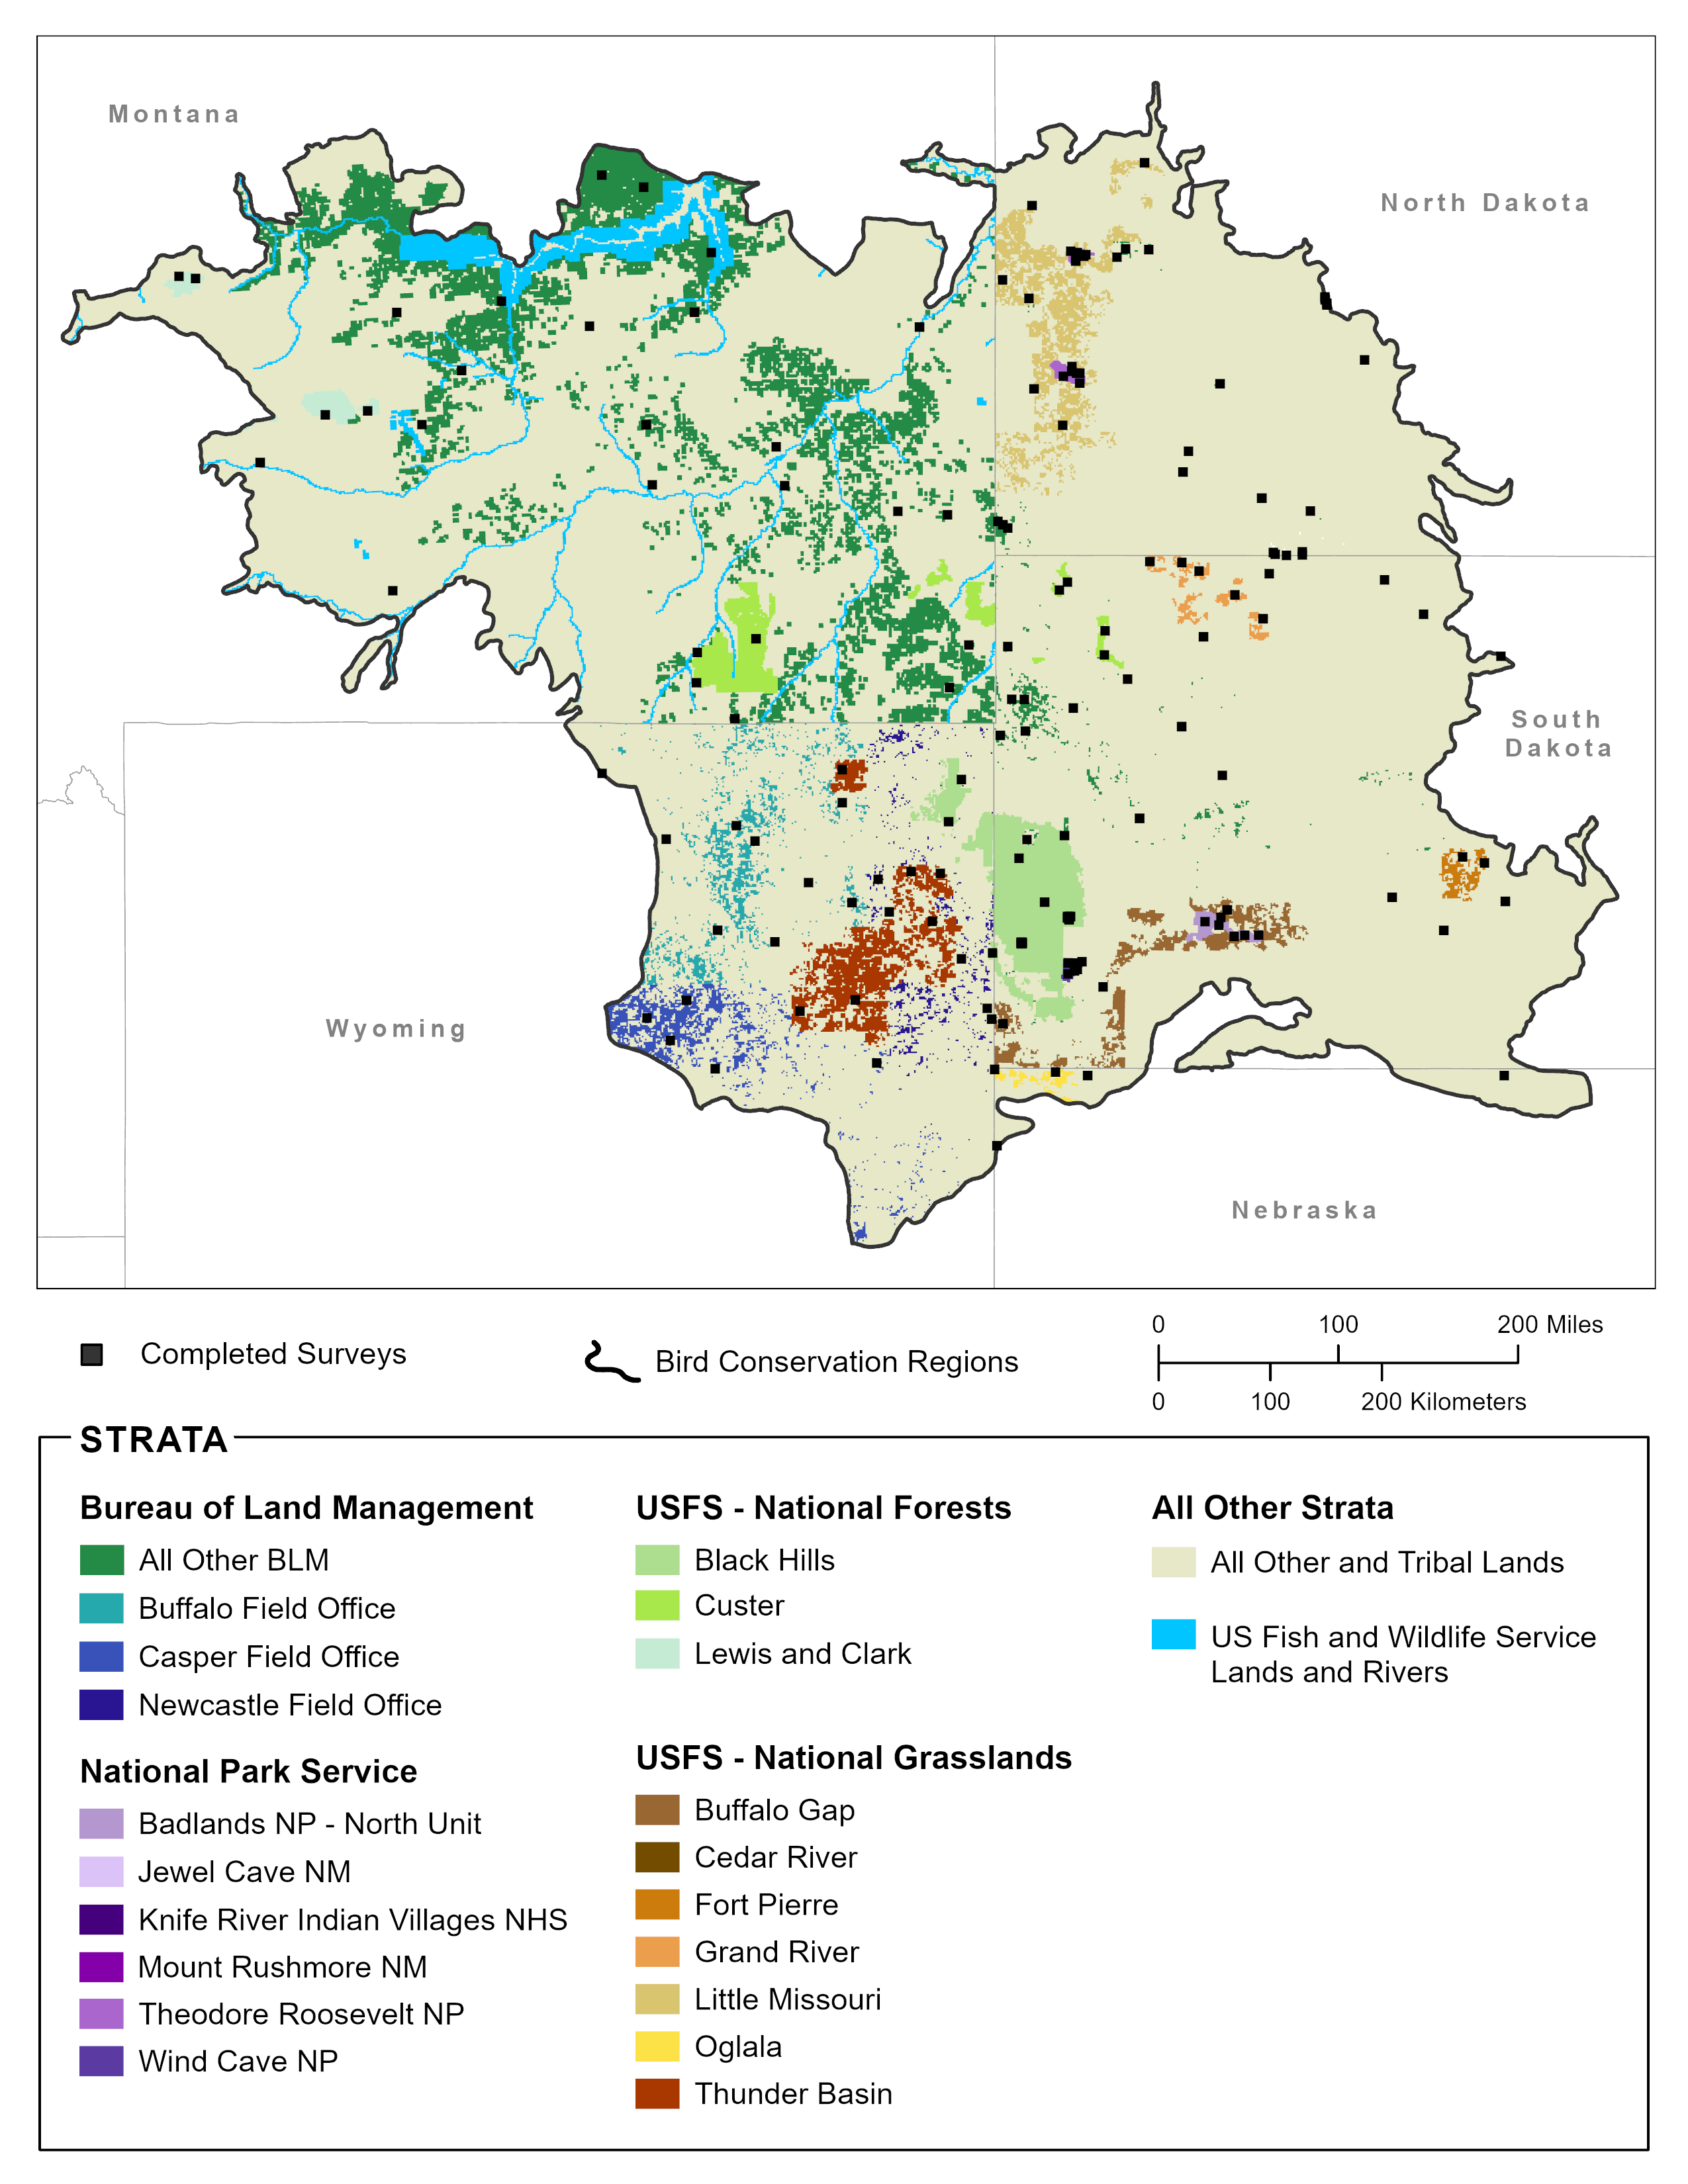
\includegraphics{./BCR17_Report_2022_NoLogo.png}

}

\caption{\label{fig-bcr-17}Survey locations and strata in the Badlands
and Prairies Bird Conservation Region (BCR 17), 2022}

\end{figure}

\hypertarget{bird-conservation-region-17}{%
\subsubsection{Bird Conservation Region
17}\label{bird-conservation-region-17}}

We obtained results for Bird Conservation Region 17 by compiling and
jointly analyzing data from 30 strata.

Field technicians completed 157 of 158 planned surveys (99\%) in 2022.
Technicians conducted 1778 point counts within the 158 surveyed grid
cells between May 24 and July 18. They detected 187 bird species,
including 45 priority species.

Bird Conservancy estimated densities and population sizes for 229
species that were detected in any year during which surveys were
conducted, 61 of which are priority species. The data yielded robust
density estimates (CV \textless{} 50\%) for 69 species.

Bird Conservancy estimated the proportion of 1 km² grid cells occupied
(Ψ, Psi) throughout Bird Conservation Region 17 for 229 species that
were detected in any year during which surveys were conducted, 61 of
which are priority species. The data yielded robust occupancy estimates
(CV \textless{} 50\%) for 120 species.

To view a map of survey locations, density and occupancy results and
species counts within Bird Conservation Region 17 across all years of
the project, follow the web link below. Hit ``Ok'' on the Rocky Mountain
Avian Data Center Disclaimer and hit the ``Run Query'' button
highlighted in red located near the top of the page (the map will zoom
to the area of interest). To view occupancy, density, or species counts
results, click on the respective tab in the upper left above the map.

\href{http://www.rmbo.org/new_site/adc/QueryWindow.aspx\#N4IgzgrgDgpgTmALnAhoiBbEAuABCAIQGEAlARgHYQBfIA==}{BCR17}

\hypertarget{colorado}{%
\chapter{Colorado}\label{colorado}}

\begin{figure}

{\centering 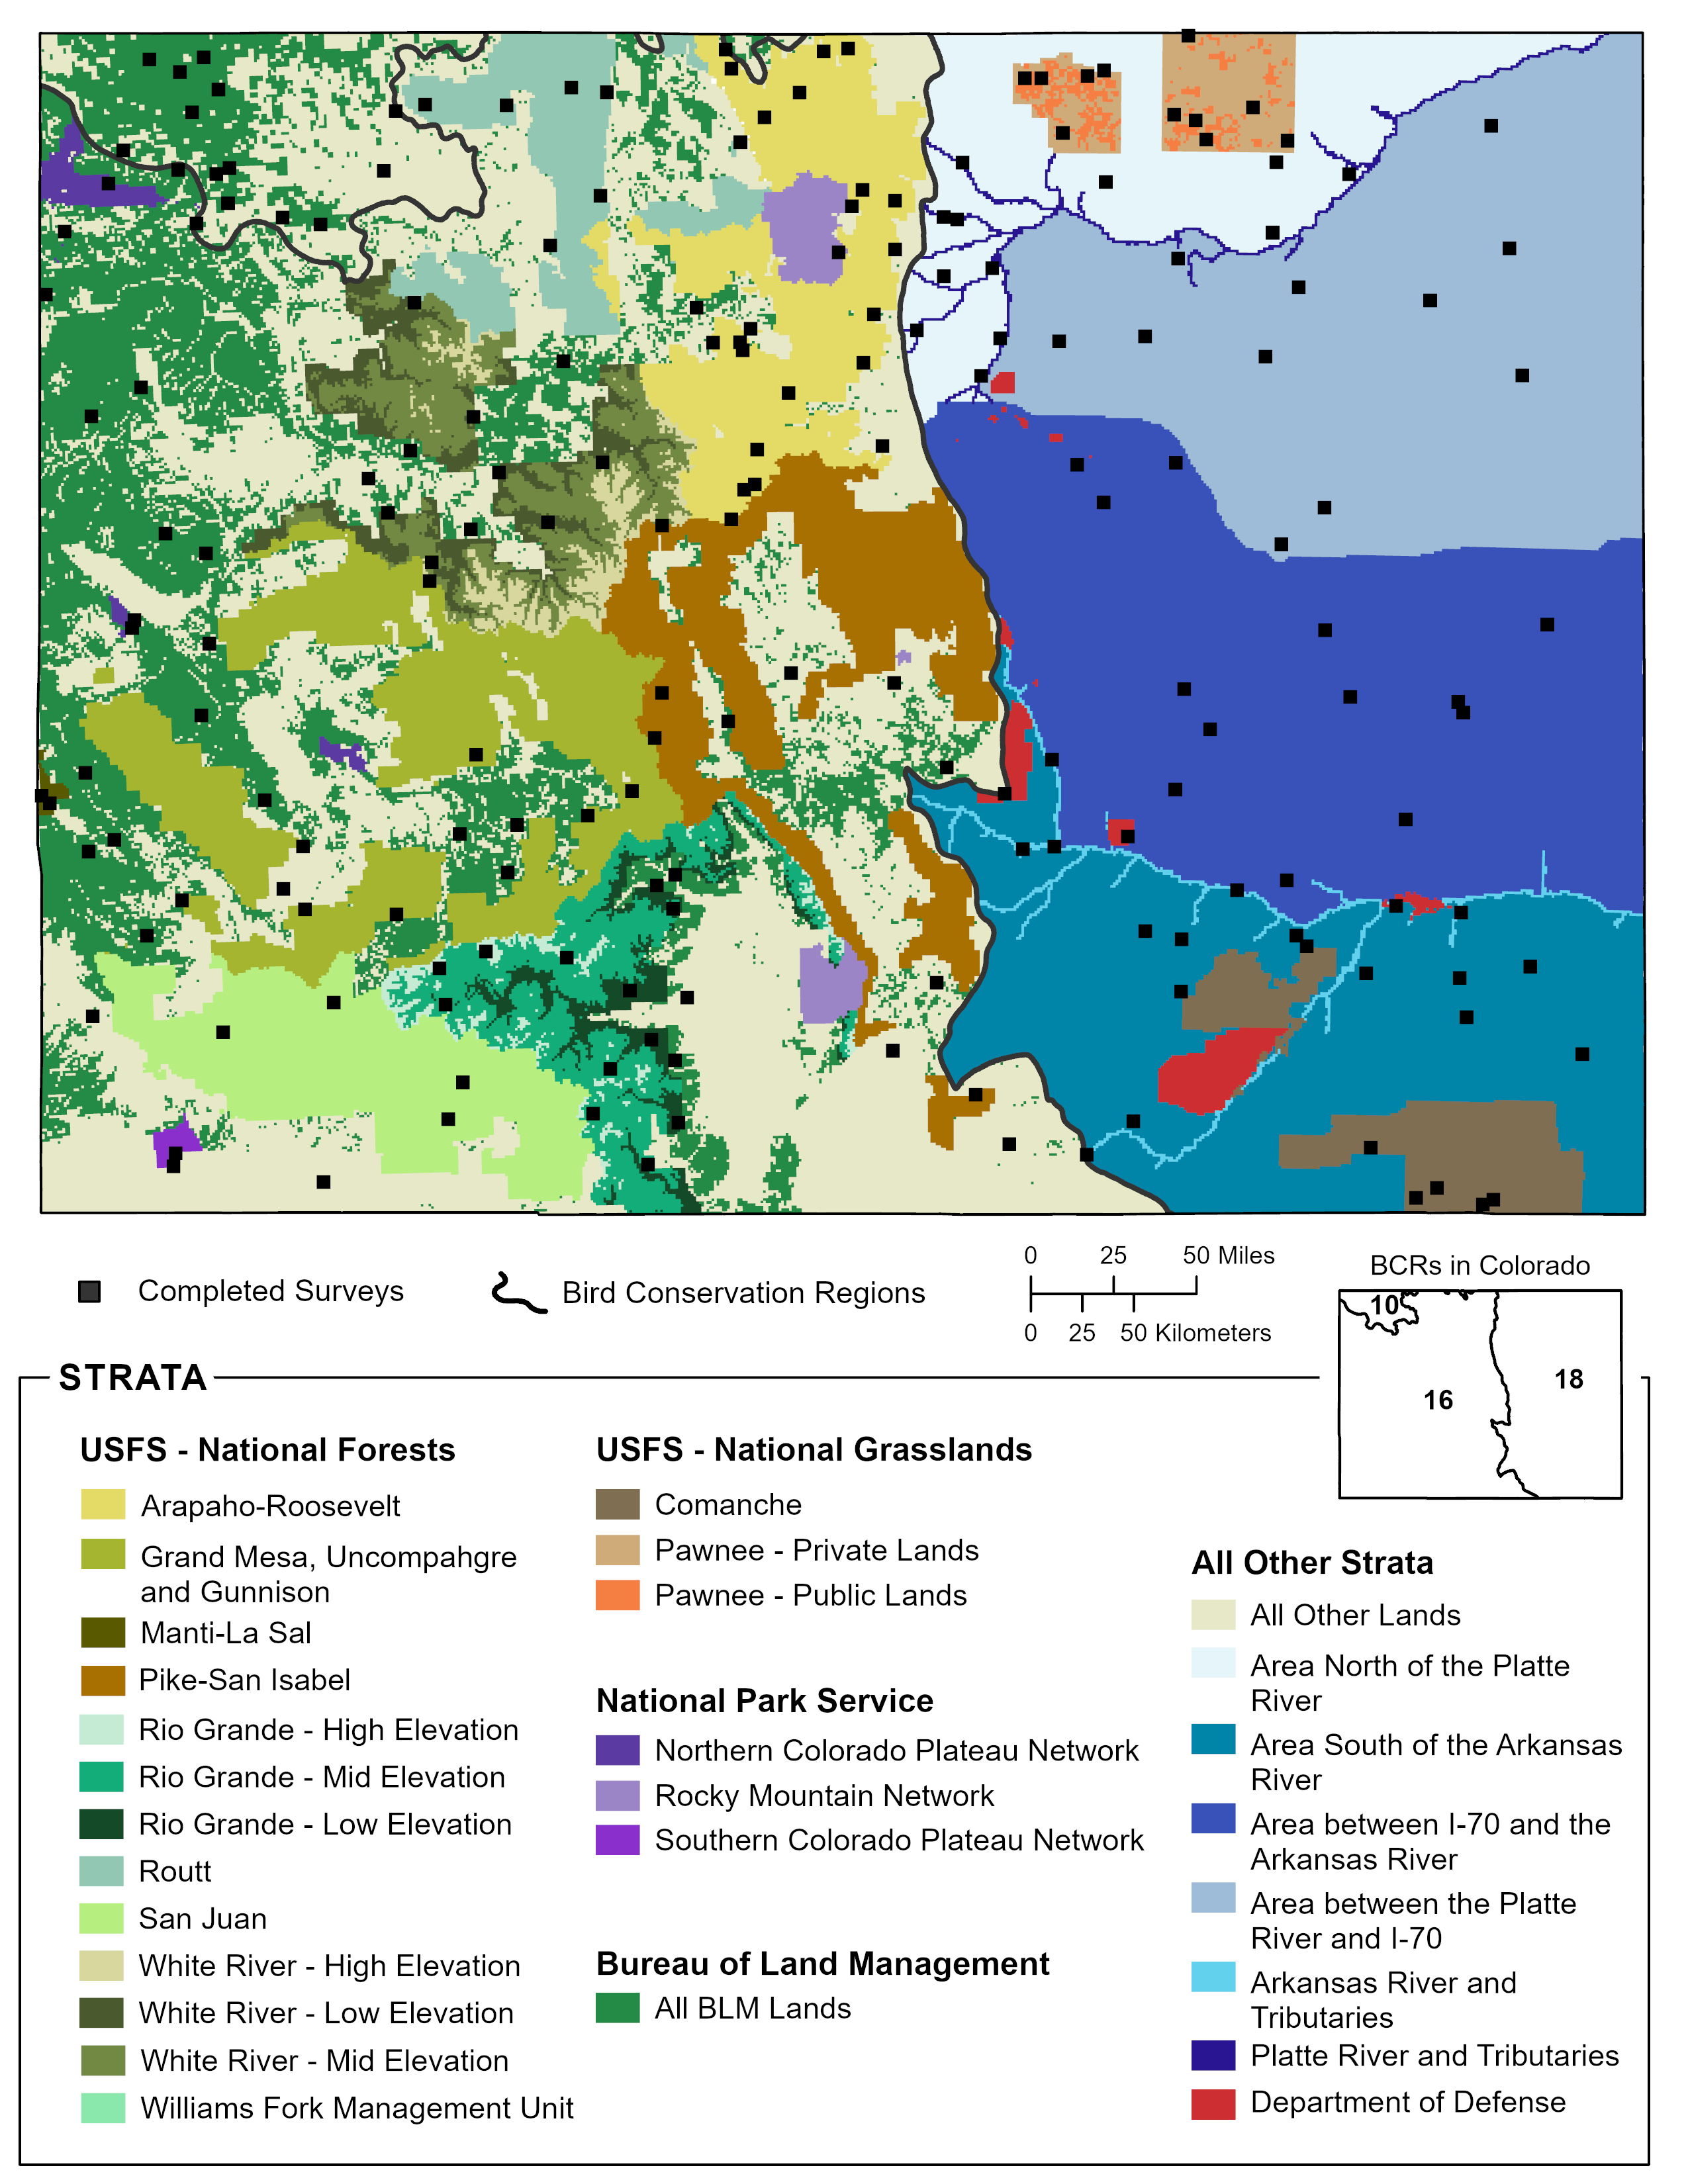
\includegraphics{./CO_Report_2022.png}

}

\caption{\label{fig-co}Survey locations and strata in Colorado, 2022.}

\end{figure}

\hypertarget{colorado-statewide-total}{%
\subsubsection{Colorado Statewide:
Total}\label{colorado-statewide-total}}

We obtained results for Colorado Statewide: Total by compiling and
jointly analyzing data from 30 strata.

Field technicians completed 213 of 193 planned surveys (110\%) in 2022.
Technicians conducted 2032 point counts within the 193 surveyed grid
cells between May 16 and July 25. They detected 202 bird species,
including 38 priority species.

Bird Conservancy estimated densities and population sizes for 237
species that were detected in any year during which surveys were
conducted, 46 of which are priority species. The data yielded robust
density estimates (CV \textless{} 50\%) for 107 species.

Bird Conservancy estimated the proportion of 1 km² grid cells occupied
(Ψ, Psi) throughout Colorado Statewide: Total for 238 species that were
detected in any year during which surveys were conducted, 46 of which
are priority species. The data yielded robust occupancy estimates (CV
\textless{} 50\%) for 156 species.

To view a map of survey locations, density and occupancy results and
species counts within Colorado Statewide: Total across all years of the
project, follow the web link below. Hit ``Ok'' on the Rocky Mountain
Avian Data Center Disclaimer and hit the ``Run Query'' button
highlighted in red located near the top of the page (the map will zoom
to the area of interest). To view occupancy, density, or species counts
results, click on the respective tab in the upper left above the map.

\href{http://www.rmbo.org/new_site/adc/QueryWindow.aspx\#N4IgzgrgDgpgTmALnAhoiBbEAuABCAYQHkQBfIA=}{CO}

\hypertarget{all-other-lands-in-colorado}{%
\subsubsection{All Other Lands in
Colorado}\label{all-other-lands-in-colorado}}

We obtained results for All Other Lands in Colorado by compiling and
jointly analyzing data from seven strata.

Field technicians completed 83 of 72 planned surveys (115\%) in 2022.
Technicians conducted 763 point counts within the 72 surveyed grid cells
between May 16 and July 21. They detected 152 bird species, including 28
priority species.

Bird Conservancy estimated densities and population sizes for 202
species that were detected in any year during which surveys were
conducted, 41 of which are priority species. The data yielded robust
density estimates (CV \textless{} 50\%) for 83 species.

Bird Conservancy estimated the proportion of 1 km² grid cells occupied
(Ψ, Psi) throughout All Other Lands in Colorado for 203 species that
were detected in any year during which surveys were conducted, 43 of
which are priority species. The data yielded robust occupancy estimates
(CV \textless{} 50\%) for 111 species.

To view a map of survey locations, density and occupancy results and
species counts within All Other Lands in Colorado across all years of
the project, follow the web link below. Hit ``Ok'' on the Rocky Mountain
Avian Data Center Disclaimer and hit the ``Run Query'' button
highlighted in red located near the top of the page (the map will zoom
to the area of interest). To view occupancy, density, or species counts
results, click on the respective tab in the upper left above the map.

\href{http://www.rmbo.org/new_site/adc/QueryWindow.aspx\#N4IgzgrgDgpgTmALnAhoiBbEAuABCAYQHkBaAQQBsLcjEALeEAXyA===}{CO-All
Other}

\hypertarget{colorado-bcr-10}{%
\section{Colorado BCR 10}\label{colorado-bcr-10}}

\hypertarget{colorado-bcr-10-total}{%
\subsubsection{Colorado BCR 10: Total}\label{colorado-bcr-10-total}}

We obtained results for Colorado BCR 10: Total by compiling and jointly
analyzing data from two strata.

Field technicians completed all planned surveys (100\%) in 2022.
Technicians conducted 182 point counts within the 14 surveyed grid cells
between May 18 and June 13. They detected 75 bird species, including 13
priority species.

Bird Conservancy estimated densities and population sizes for 127
species that were detected in any year during which surveys were
conducted, 26 of which are priority species. The data yielded robust
density estimates (CV \textless{} 50\%) for 32 species.

Bird Conservancy estimated the proportion of 1 km² grid cells occupied
(Ψ, Psi) throughout Colorado BCR 10: Total for 124 species that were
detected in any year during which surveys were conducted, 23 of which
are priority species. The data yielded robust occupancy estimates (CV
\textless{} 50\%) for 50 species.

To view a map of survey locations, density and occupancy results and
species counts within Colorado BCR 10: Total across all years of the
project, follow the web link below. Hit ``Ok'' on the Rocky Mountain
Avian Data Center Disclaimer and hit the ``Run Query'' button
highlighted in red located near the top of the page (the map will zoom
to the area of interest). To view occupancy, density, or species counts
results, click on the respective tab in the upper left above the map.

\href{http://www.rmbo.org/new_site/adc/QueryWindow.aspx\#N4IgzgrgDgpgTmALnAhoiBbEAuABCAYQHkBaAIQICUBGABhAF8g=}{CO-BCR10}

\hypertarget{all-other-lands-in-colorado-bcr-10}{%
\subsubsection{All Other Lands in Colorado BCR
10}\label{all-other-lands-in-colorado-bcr-10}}

We obtained results for All Other Lands in Colorado BCR 10 by compiling
and analyzing data from one stratum.

Field technicians completed all planned surveys (100\%) in 2022.
Technicians conducted 55 point counts within the 5 surveyed grid cells
between May 21 and June 13. They detected 62 bird species, including 6
priority species.

Bird Conservancy estimated densities and population sizes for 111
species that were detected in any year during which surveys were
conducted, 21 of which are priority species. The data yielded robust
density estimates (CV \textless{} 50\%) for 25 species.

Bird Conservancy estimated the proportion of 1 km² grid cells occupied
(Ψ, Psi) throughout All Other Lands in Colorado BCR 10 for 110 species
that were detected in any year during which surveys were conducted, 19
of which are priority species. The data yielded robust occupancy
estimates (CV \textless{} 50\%) for 38 species.

To view a map of survey locations, density and occupancy results and
species counts within All Other Lands in Colorado BCR 10 across all
years of the project, follow the web link below. Hit ``Ok'' on the Rocky
Mountain Avian Data Center Disclaimer and hit the ``Run Query'' button
highlighted in red located near the top of the page (the map will zoom
to the area of interest). To view occupancy, density, or species counts
results, click on the respective tab in the upper left above the map.

\href{http://www.rmbo.org/new_site/adc/QueryWindow.aspx\#N4IgzgLgTghhCuBbEAuABCAwgeQLQCFMAlARgAZcBBbdSgGzrWwgAsBTKNAGRgDsATMCAC+QA===}{CO-BCR10-AO}

\hypertarget{colorado-bcr-16}{%
\section{Colorado BCR 16}\label{colorado-bcr-16}}

\hypertarget{colorado-bcr-16-total}{%
\subsubsection{Colorado BCR 16: Total}\label{colorado-bcr-16-total}}

We obtained results for Colorado BCR 16: Total by compiling and jointly
analyzing data from 18 strata.

Field technicians completed 120 of 108 planned surveys (111\%) in 2022.
Technicians conducted 1050 point counts within the 108 surveyed grid
cells between May 17 and July 25. They detected 153 bird species,
including 24 priority species.

Bird Conservancy estimated densities and population sizes for 200
species that were detected in any year during which surveys were
conducted, 35 of which are priority species. The data yielded robust
density estimates (CV \textless{} 50\%) for 86 species.

Bird Conservancy estimated the proportion of 1 km² grid cells occupied
(Ψ, Psi) throughout Colorado BCR 16: Total for 198 species that were
detected in any year during which surveys were conducted, 35 of which
are priority species. The data yielded robust occupancy estimates (CV
\textless{} 50\%) for 123 species.

To view a map of survey locations, density and occupancy results and
species counts within Colorado BCR 16: Total across all years of the
project, follow the web link below. Hit ``Ok'' on the Rocky Mountain
Avian Data Center Disclaimer and hit the ``Run Query'' button
highlighted in red located near the top of the page (the map will zoom
to the area of interest). To view occupancy, density, or species counts
results, click on the respective tab in the upper left above the map.

\href{http://www.rmbo.org/new_site/adc/QueryWindow.aspx\#N4IgzgrgDgpgTmALnAhoiBbEAuABCAYQHkBaAIQICUBGANhAF8g=}{CO-BCR16}

\hypertarget{all-other-lands-in-colorado-bcr-16}{%
\subsubsection{All Other Lands in Colorado BCR
16}\label{all-other-lands-in-colorado-bcr-16}}

We obtained results for All Other Lands in Colorado BCR 16 by compiling
and analyzing data from one stratum.

Field technicians completed 25 of 22 planned surveys (114\%) in 2022.
Technicians conducted 190 point counts within the 22 surveyed grid cells
between May 17 and July 21. They detected 116 bird species, including 16
priority species.

Bird Conservancy estimated densities and population sizes for 178
species that were detected in any year during which surveys were
conducted, 33 of which are priority species. The data yielded robust
density estimates (CV \textless{} 50\%) for 64 species.

Bird Conservancy estimated the proportion of 1 km² grid cells occupied
(Ψ, Psi) throughout All Other Lands in Colorado BCR 16 for 174 species
that were detected in any year during which surveys were conducted, 33
of which are priority species. The data yielded robust occupancy
estimates (CV \textless{} 50\%) for 86 species.

To view a map of survey locations, density and occupancy results and
species counts within All Other Lands in Colorado BCR 16 across all
years of the project, follow the web link below. Hit ``Ok'' on the Rocky
Mountain Avian Data Center Disclaimer and hit the ``Run Query'' button
highlighted in red located near the top of the page (the map will zoom
to the area of interest). To view occupancy, density, or species counts
results, click on the respective tab in the upper left above the map.

\href{http://www.rmbo.org/new_site/adc/QueryWindow.aspx\#N4IgzgLgTghhCuBbEAuABCAwgeQLQCFMAlARgDZcBBbdSgGzrWwgAsBTKNAGRgDsATMCAC+QA===}{CO-BCR16-AO}

\hypertarget{colorado-bcr-18}{%
\section{Colorado BCR 18}\label{colorado-bcr-18}}

\hypertarget{colorado-bcr-18-total}{%
\subsubsection{Colorado BCR 18: Total}\label{colorado-bcr-18-total}}

We obtained results for Colorado BCR 18: Total by compiling and jointly
analyzing data from five strata.

Field technicians completed 53 of 45 planned surveys (118\%) in 2022.
Technicians conducted 518 point counts within the 45 surveyed grid cells
between May 16 and June 15. They detected 84 bird species, including 14
priority species.

Bird Conservancy estimated densities and population sizes for 132
species that were detected in any year during which surveys were
conducted, 23 of which are priority species. The data yielded robust
density estimates (CV \textless{} 50\%) for 32 species.

Bird Conservancy estimated the proportion of 1 km² grid cells occupied
(Ψ, Psi) throughout Colorado BCR 18: Total for 131 species that were
detected in any year during which surveys were conducted, 22 of which
are priority species. The data yielded robust occupancy estimates (CV
\textless{} 50\%) for 49 species.

To view a map of survey locations, density and occupancy results and
species counts within Colorado BCR 18: Total across all years of the
project, follow the web link below. Hit ``Ok'' on the Rocky Mountain
Avian Data Center Disclaimer and hit the ``Run Query'' button
highlighted in red located near the top of the page (the map will zoom
to the area of interest). To view occupancy, density, or species counts
results, click on the respective tab in the upper left above the map.

\href{http://www.rmbo.org/new_site/adc/QueryWindow.aspx\#N4IgzgrgDgpgTmALnAhoiBbEAuABCAYQHkBaAIQICUBGADhIEEAbJ3IxAC3hAF8g}{CO-BCR18-All
Other}

\hypertarget{colorado-bcr-18-rivers}{%
\subsubsection{Colorado BCR 18 Rivers}\label{colorado-bcr-18-rivers}}

We obtained results for Colorado BCR 18 Rivers by compiling and jointly
analyzing data from two strata.

Field technicians completed all planned surveys (100\%) in 2022.
Technicians conducted 101 point counts within the 11 surveyed grid cells
between May 17 and June 22. They detected 90 bird species, including 7
priority species.

Bird Conservancy estimated densities and population sizes for 176
species that were detected in any year during which surveys were
conducted, 25 of which are priority species. The data yielded robust
density estimates (CV \textless{} 50\%) for 35 species.

Bird Conservancy estimated the proportion of 1 km² grid cells occupied
(Ψ, Psi) throughout Colorado BCR 18 Rivers for 172 species that were
detected in any year during which surveys were conducted, 24 of which
are priority species. The data yielded robust occupancy estimates (CV
\textless{} 50\%) for 72 species.

To view a map of survey locations, density and occupancy results and
species counts within Colorado BCR 18 Rivers across all years of the
project, follow the web link below. Hit ``Ok'' on the Rocky Mountain
Avian Data Center Disclaimer and hit the ``Run Query'' button
highlighted in red located near the top of the page (the map will zoom
to the area of interest). To view occupancy, density, or species counts
results, click on the respective tab in the upper left above the map.

\href{http://www.rmbo.org/new_site/adc/QueryWindow.aspx\#N4IgzgrgDgpgTmALnAhoiBbEAuABCAYQHkBaAJQEsA3eMEAXyA==}{CO-Rivers}

\hypertarget{non-river-lands-in-colorado-bcr-18}{%
\subsubsection{Non-river Lands in Colorado BCR
18}\label{non-river-lands-in-colorado-bcr-18}}

We obtained results for Non-river Lands in Colorado BCR 18 by compiling
and jointly analyzing data from eight strata.

Field technicians completed 68 of 60 planned surveys (113\%) in 2022.
Technicians conducted 699 point counts within the 60 surveyed grid cells
between May 16 and June 15. They detected 108 bird species, including 16
priority species.

Bird Conservancy estimated densities and population sizes for 166
species that were detected in any year during which surveys were
conducted, 28 of which are priority species. The data yielded robust
density estimates (CV \textless{} 50\%) for 44 species.

Bird Conservancy estimated the proportion of 1 km² grid cells occupied
(Ψ, Psi) throughout Non-river Lands in Colorado BCR 18 for 164 species
that were detected in any year during which surveys were conducted, 27
of which are priority species. The data yielded robust occupancy
estimates (CV \textless{} 50\%) for 59 species.

To view a map of survey locations, density and occupancy results and
species counts within Non-river Lands in Colorado BCR 18 across all
years of the project, follow the web link below. Hit ``Ok'' on the Rocky
Mountain Avian Data Center Disclaimer and hit the ``Run Query'' button
highlighted in red located near the top of the page (the map will zoom
to the area of interest). To view occupancy, density, or species counts
results, click on the respective tab in the upper left above the map.

\href{http://www.rmbo.org/new_site/adc/QueryWindow.aspx\#N4IgzgrgDgpgTmALnAhoiBbEAuABCAYQHkBaAIQICUBGADhIDkB7AOzgEsA3eMEAXyA=}{CO-BCR18-Nonrivers}

\hypertarget{montana}{%
\chapter{Montana}\label{montana}}

\begin{figure}

{\centering 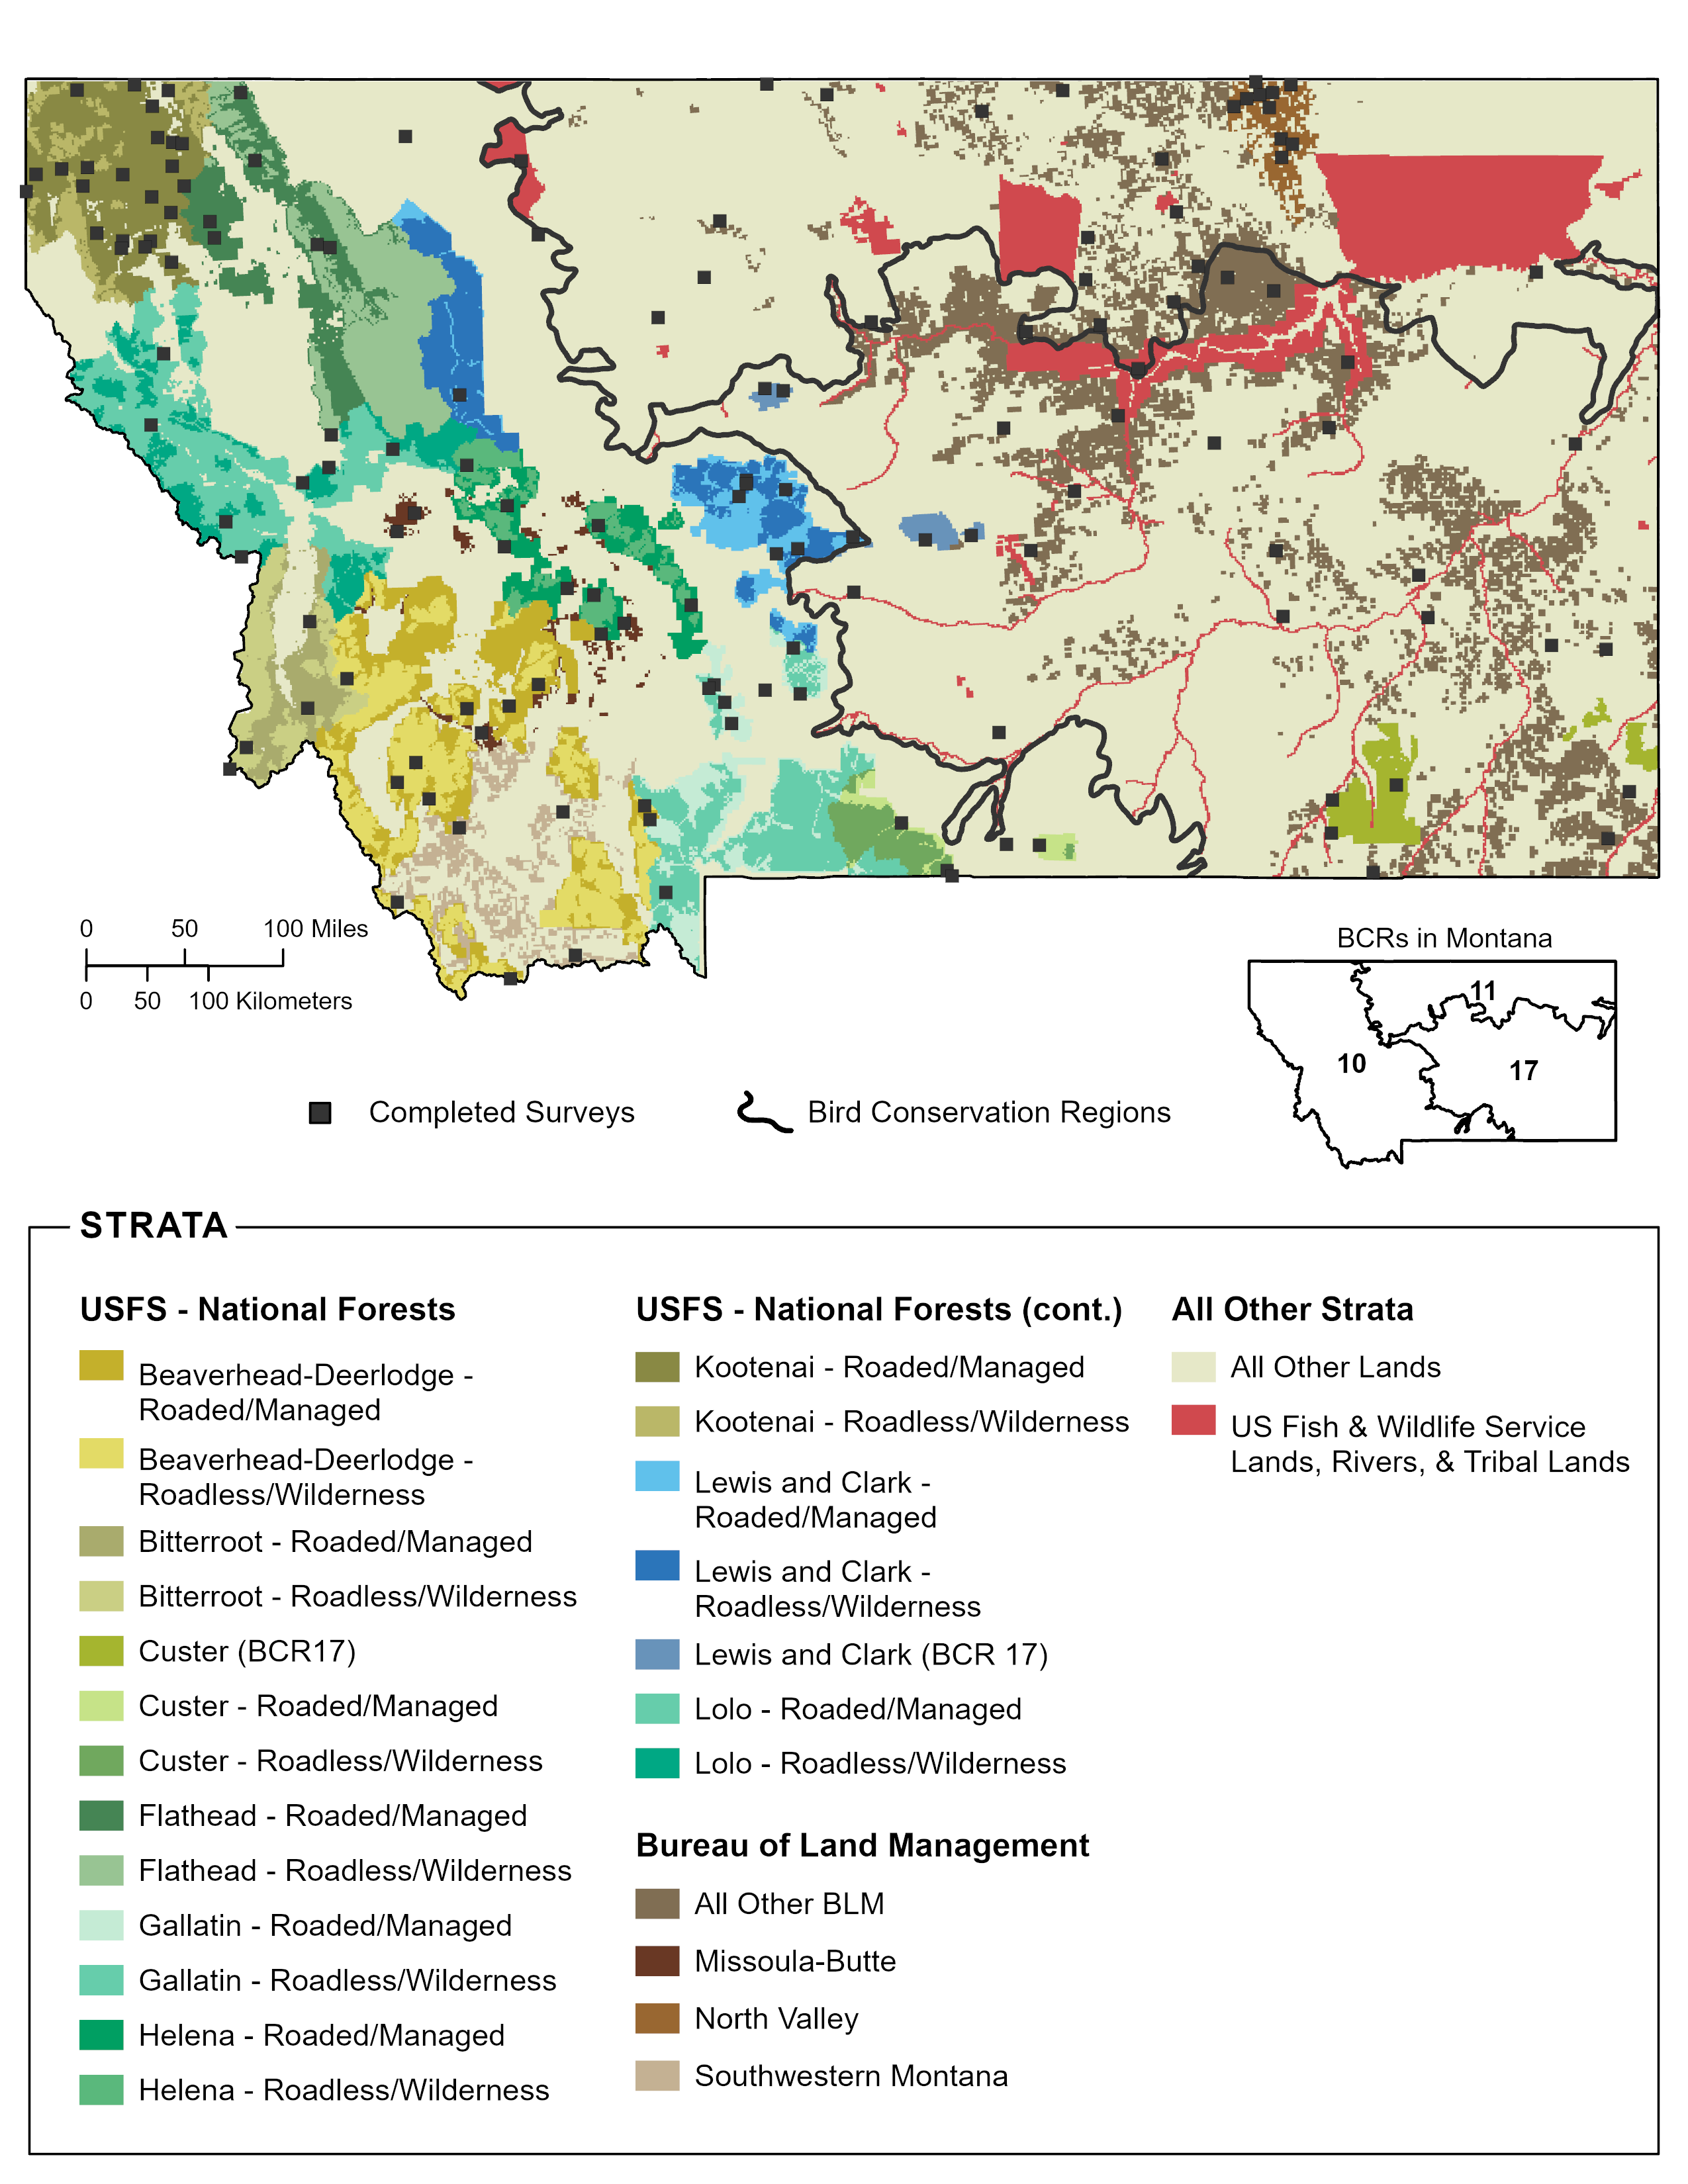
\includegraphics{./MT_Report_2022_NoLogo.png}

}

\caption{\label{fig-mt}Survey locations and strata in Montana, 2022.}

\end{figure}

\hypertarget{montana-statewide-total}{%
\subsubsection{Montana Statewide: Total}\label{montana-statewide-total}}

We obtained results for Montana Statewide: Total by compiling and
jointly analyzing data from 30 strata.

Field technicians completed 159 of 156 planned surveys (102\%) in 2022.
Technicians conducted 1850 point counts within the 156 surveyed grid
cells between May 28 and July 15. They detected 196 bird species,
including 34 priority species.

Bird Conservancy estimated densities and population sizes for 218
species that were detected in any year during which surveys were
conducted, 40 of which are priority species. The data yielded robust
density estimates (CV \textless{} 50\%) for 92 species.

Bird Conservancy estimated the proportion of 1 km² grid cells occupied
(Ψ, Psi) throughout Montana Statewide: Total for 223 species that were
detected in any year during which surveys were conducted, 42 of which
are priority species. The data yielded robust occupancy estimates (CV
\textless{} 50\%) for 153 species.

To view a map of survey locations, density and occupancy results and
species counts within Montana Statewide: Total across all years of the
project, follow the web link below. Hit ``Ok'' on the Rocky Mountain
Avian Data Center Disclaimer and hit the ``Run Query'' button
highlighted in red located near the top of the page (the map will zoom
to the area of interest). To view occupancy, density, or species counts
results, click on the respective tab in the upper left above the map.

\href{http://www.rmbo.org/new_site/adc/QueryWindow.aspx\#N4IgzgrgDgpgTmALnAhoiBbEAuABCAWQBUQBfIA=}{MT}

\hypertarget{all-other-lands-in-montana}{%
\subsubsection{All Other Lands in
Montana}\label{all-other-lands-in-montana}}

We obtained results for All Other Lands in Montana by compiling and
jointly analyzing data from three strata.

Field technicians completed all planned surveys (100\%) in 2022.
Technicians conducted 330 point counts within the 24 surveyed grid cells
between June 2 and July 14. They detected 140 bird species, including 23
priority species.

Bird Conservancy estimated densities and population sizes for 186
species that were detected in any year during which surveys were
conducted, 29 of which are priority species. The data yielded robust
density estimates (CV \textless{} 50\%) for 54 species.

Bird Conservancy estimated the proportion of 1 km² grid cells occupied
(Ψ, Psi) throughout All Other Lands in Montana for 192 species that were
detected in any year during which surveys were conducted, 33 of which
are priority species. The data yielded robust occupancy estimates (CV
\textless{} 50\%) for 105 species.

To view a map of survey locations, density and occupancy results and
species counts within All Other Lands in Montana across all years of the
project, follow the web link below. Hit ``Ok'' on the Rocky Mountain
Avian Data Center Disclaimer and hit the ``Run Query'' button
highlighted in red located near the top of the page (the map will zoom
to the area of interest). To view occupancy, density, or species counts
results, click on the respective tab in the upper left above the map.

\href{http://www.rmbo.org/new_site/adc/QueryWindow.aspx\#N4IgzgrgDgpgTmALnAhoiBbEAuABCAWQBUBaAQQBsLcB5RAC3hAF8g==}{MT-All
Other}

\hypertarget{montana-bcr-10}{%
\section{Montana BCR 10}\label{montana-bcr-10}}

\hypertarget{montana-bcr-10-total}{%
\subsubsection{Montana BCR 10: Total}\label{montana-bcr-10-total}}

We obtained results for Montana BCR 10: Total by compiling and jointly
analyzing data from 21 strata.

Field technicians completed 102 of 99 planned surveys (103\%) in 2022.
Technicians conducted 1054 point counts within the 99 surveyed grid
cells between May 28 and July 15. They detected 147 bird species,
including 19 priority species.

Bird Conservancy estimated densities and population sizes for 198
species that were detected in any year during which surveys were
conducted, 33 of which are priority species. The data yielded robust
density estimates (CV \textless{} 50\%) for 74 species.

Bird Conservancy estimated the proportion of 1 km² grid cells occupied
(Ψ, Psi) throughout Montana BCR 10: Total for 202 species that were
detected in any year during which surveys were conducted, 35 of which
are priority species. The data yielded robust occupancy estimates (CV
\textless{} 50\%) for 117 species.

To view a map of survey locations, density and occupancy results and
species counts within Montana BCR 10: Total across all years of the
project, follow the web link below. Hit ``Ok'' on the Rocky Mountain
Avian Data Center Disclaimer and hit the ``Run Query'' button
highlighted in red located near the top of the page (the map will zoom
to the area of interest). To view occupancy, density, or species counts
results, click on the respective tab in the upper left above the map.

\href{http://www.rmbo.org/new_site/adc/QueryWindow.aspx\#N4IgzgrgDgpgTmALnAhoiBbEAuABCAWQBUBaAIQGEAlARgAYQBfIA===}{MT-BCR10}

\hypertarget{all-other-lands-in-montana-bcr-10}{%
\subsubsection{All Other Lands in Montana BCR
10}\label{all-other-lands-in-montana-bcr-10}}

We obtained results for All Other Lands in Montana BCR 10 by compiling
and analyzing data from one stratum.

Field technicians completed all planned surveys (100\%) in 2022.
Technicians conducted 70 point counts within the 6 surveyed grid cells
between June 3 and July 14. They detected 94 bird species, including 10
priority species.

Bird Conservancy estimated densities and population sizes for 126
species that were detected in any year during which surveys were
conducted, 12 of which are priority species. The data yielded robust
density estimates (CV \textless{} 50\%) for 35 species.

Bird Conservancy estimated the proportion of 1 km² grid cells occupied
(Ψ, Psi) throughout All Other Lands in Montana BCR 10 for 124 species
that were detected in any year during which surveys were conducted, 12
of which are priority species. The data yielded robust occupancy
estimates (CV \textless{} 50\%) for 39 species.

To view a map of survey locations, density and occupancy results and
species counts within All Other Lands in Montana BCR 10 across all years
of the project, follow the web link below. Hit ``Ok'' on the Rocky
Mountain Avian Data Center Disclaimer and hit the ``Run Query'' button
highlighted in red located near the top of the page (the map will zoom
to the area of interest). To view occupancy, density, or species counts
results, click on the respective tab in the upper left above the map.

\href{http://www.rmbo.org/new_site/adc/QueryWindow.aspx\#N4IgzgLgTghhCuBbEAuABCAsgFQLQCEBhAJQEYAGXAeQDl0BBAG0bSogAsBTKNAGRgB2AEzAgAvkA===}{MT-BCR10-ON}

\hypertarget{montana-bcr-11}{%
\section{Montana BCR 11}\label{montana-bcr-11}}

\hypertarget{montana-bcr-11-total}{%
\subsubsection{Montana BCR 11: Total}\label{montana-bcr-11-total}}

We obtained results for Montana BCR 11: Total by compiling and jointly
analyzing data from four strata.

Field technicians completed all planned surveys (100\%) in 2022.
Technicians conducted 413 point counts within the 29 surveyed grid cells
between May 29 and July 13. They detected 101 bird species, including 21
priority species.

Bird Conservancy estimated densities and population sizes for 142
species that were detected in any year during which surveys were
conducted, 23 of which are priority species. The data yielded robust
density estimates (CV \textless{} 50\%) for 33 species.

Bird Conservancy estimated the proportion of 1 km² grid cells occupied
(Ψ, Psi) throughout Montana BCR 11: Total for 141 species that were
detected in any year during which surveys were conducted, 24 of which
are priority species. The data yielded robust occupancy estimates (CV
\textless{} 50\%) for 65 species.

To view a map of survey locations, density and occupancy results and
species counts within Montana BCR 11: Total across all years of the
project, follow the web link below. Hit ``Ok'' on the Rocky Mountain
Avian Data Center Disclaimer and hit the ``Run Query'' button
highlighted in red located near the top of the page (the map will zoom
to the area of interest). To view occupancy, density, or species counts
results, click on the respective tab in the upper left above the map.

\href{http://www.rmbo.org/new_site/adc/QueryWindow.aspx\#N4IgzgrgDgpgTmALnAhoiBbEAuABCAWQBUBaAIQGEAlARhpAF8g=}{MT-BCR11}

\hypertarget{all-other-lands-in-montana-bcr-11}{%
\subsubsection{All Other Lands in Montana BCR
11}\label{all-other-lands-in-montana-bcr-11}}

We obtained results for All Other Lands in Montana BCR 11 by compiling
and analyzing data from one stratum.

Field technicians completed all planned surveys (100\%) in 2022.
Technicians conducted 129 point counts within the 9 surveyed grid cells
between June 11 and July 7. They detected 77 bird species, including 17
priority species.

Bird Conservancy estimated densities and population sizes for 116
species that were detected in any year during which surveys were
conducted, 19 of which are priority species. The data yielded robust
density estimates (CV \textless{} 50\%) for 26 species.

Bird Conservancy estimated the proportion of 1 km² grid cells occupied
(Ψ, Psi) throughout All Other Lands in Montana BCR 11 for 114 species
that were detected in any year during which surveys were conducted, 19
of which are priority species. The data yielded robust occupancy
estimates (CV \textless{} 50\%) for 43 species.

To view a map of survey locations, density and occupancy results and
species counts within All Other Lands in Montana BCR 11 across all years
of the project, follow the web link below. Hit ``Ok'' on the Rocky
Mountain Avian Data Center Disclaimer and hit the ``Run Query'' button
highlighted in red located near the top of the page (the map will zoom
to the area of interest). To view occupancy, density, or species counts
results, click on the respective tab in the upper left above the map.

\href{http://www.rmbo.org/new_site/adc/QueryWindow.aspx\#N4IgzgLgTghhCuBbEAuABCAsgFQLQCEBhAJQEZTcBBAeXUoBt61qIALAUyjQBkYA7ACZgQAXyA==}{MT-BCR11-AO}

\hypertarget{montana-bcr-17}{%
\section{Montana BCR 17}\label{montana-bcr-17}}

\hypertarget{montana-bcr-17-total}{%
\subsubsection{Montana BCR 17: Total}\label{montana-bcr-17-total}}

We obtained results for Montana BCR 17: Total by compiling and jointly
analyzing data from five strata.

Field technicians completed all planned surveys (100\%) in 2022.
Technicians conducted 383 point counts within the 28 surveyed grid cells
between June 1 and July 8. They detected 121 bird species, including 16
priority species.

Bird Conservancy estimated densities and population sizes for 192
species that were detected in any year during which surveys were
conducted, 31 of which are priority species. The data yielded robust
density estimates (CV \textless{} 50\%) for 50 species.

Bird Conservancy estimated the proportion of 1 km² grid cells occupied
(Ψ, Psi) throughout Montana BCR 17: Total for 190 species that were
detected in any year during which surveys were conducted, 30 of which
are priority species. The data yielded robust occupancy estimates (CV
\textless{} 50\%) for 81 species.

To view a map of survey locations, density and occupancy results and
species counts within Montana BCR 17: Total across all years of the
project, follow the web link below. Hit ``Ok'' on the Rocky Mountain
Avian Data Center Disclaimer and hit the ``Run Query'' button
highlighted in red located near the top of the page (the map will zoom
to the area of interest). To view occupancy, density, or species counts
results, click on the respective tab in the upper left above the map.

\href{http://www.rmbo.org/new_site/adc/QueryWindow.aspx\#N4IgzgrgDgpgTmALnAhoiBbEAuABCAWQBUBaAIQGEAlARgHYQBfIA===}{MT-BCR17}

\hypertarget{all-other-lands-in-montana-bcr-17}{%
\subsubsection{All Other Lands in Montana BCR
17}\label{all-other-lands-in-montana-bcr-17}}

We obtained results for All Other Lands in Montana BCR 17 by compiling
and analyzing data from one stratum.

Field technicians completed all planned surveys (100\%) in 2022.
Technicians conducted 131 point counts within the 9 surveyed grid cells
between June 2 and July 8. They detected 66 bird species, including 15
priority species.

Bird Conservancy estimated densities and population sizes for 131
species that were detected in any year during which surveys were
conducted, 18 of which are priority species. The data yielded robust
density estimates (CV \textless{} 50\%) for 28 species.

Bird Conservancy estimated the proportion of 1 km² grid cells occupied
(Ψ, Psi) throughout All Other Lands in Montana BCR 17 for 127 species
that were detected in any year during which surveys were conducted, 17
of which are priority species. The data yielded robust occupancy
estimates (CV \textless{} 50\%) for 43 species.

To view a map of survey locations, density and occupancy results and
species counts within All Other Lands in Montana BCR 17 across all years
of the project, follow the web link below. Hit ``Ok'' on the Rocky
Mountain Avian Data Center Disclaimer and hit the ``Run Query'' button
highlighted in red located near the top of the page (the map will zoom
to the area of interest). To view occupancy, density, or species counts
results, click on the respective tab in the upper left above the map.

\href{http://www.rmbo.org/new_site/adc/QueryWindow.aspx\#N4IgzgLgTghhCuBbEAuABCAsgFQLQCEBhAJQEYB2XAQQHl0qAbBtGiACwFMo0AZGAOwAmYEAF8gA}{MT-BCR17-AO}

\hypertarget{utah}{%
\chapter{Utah}\label{utah}}

\begin{figure}

{\centering 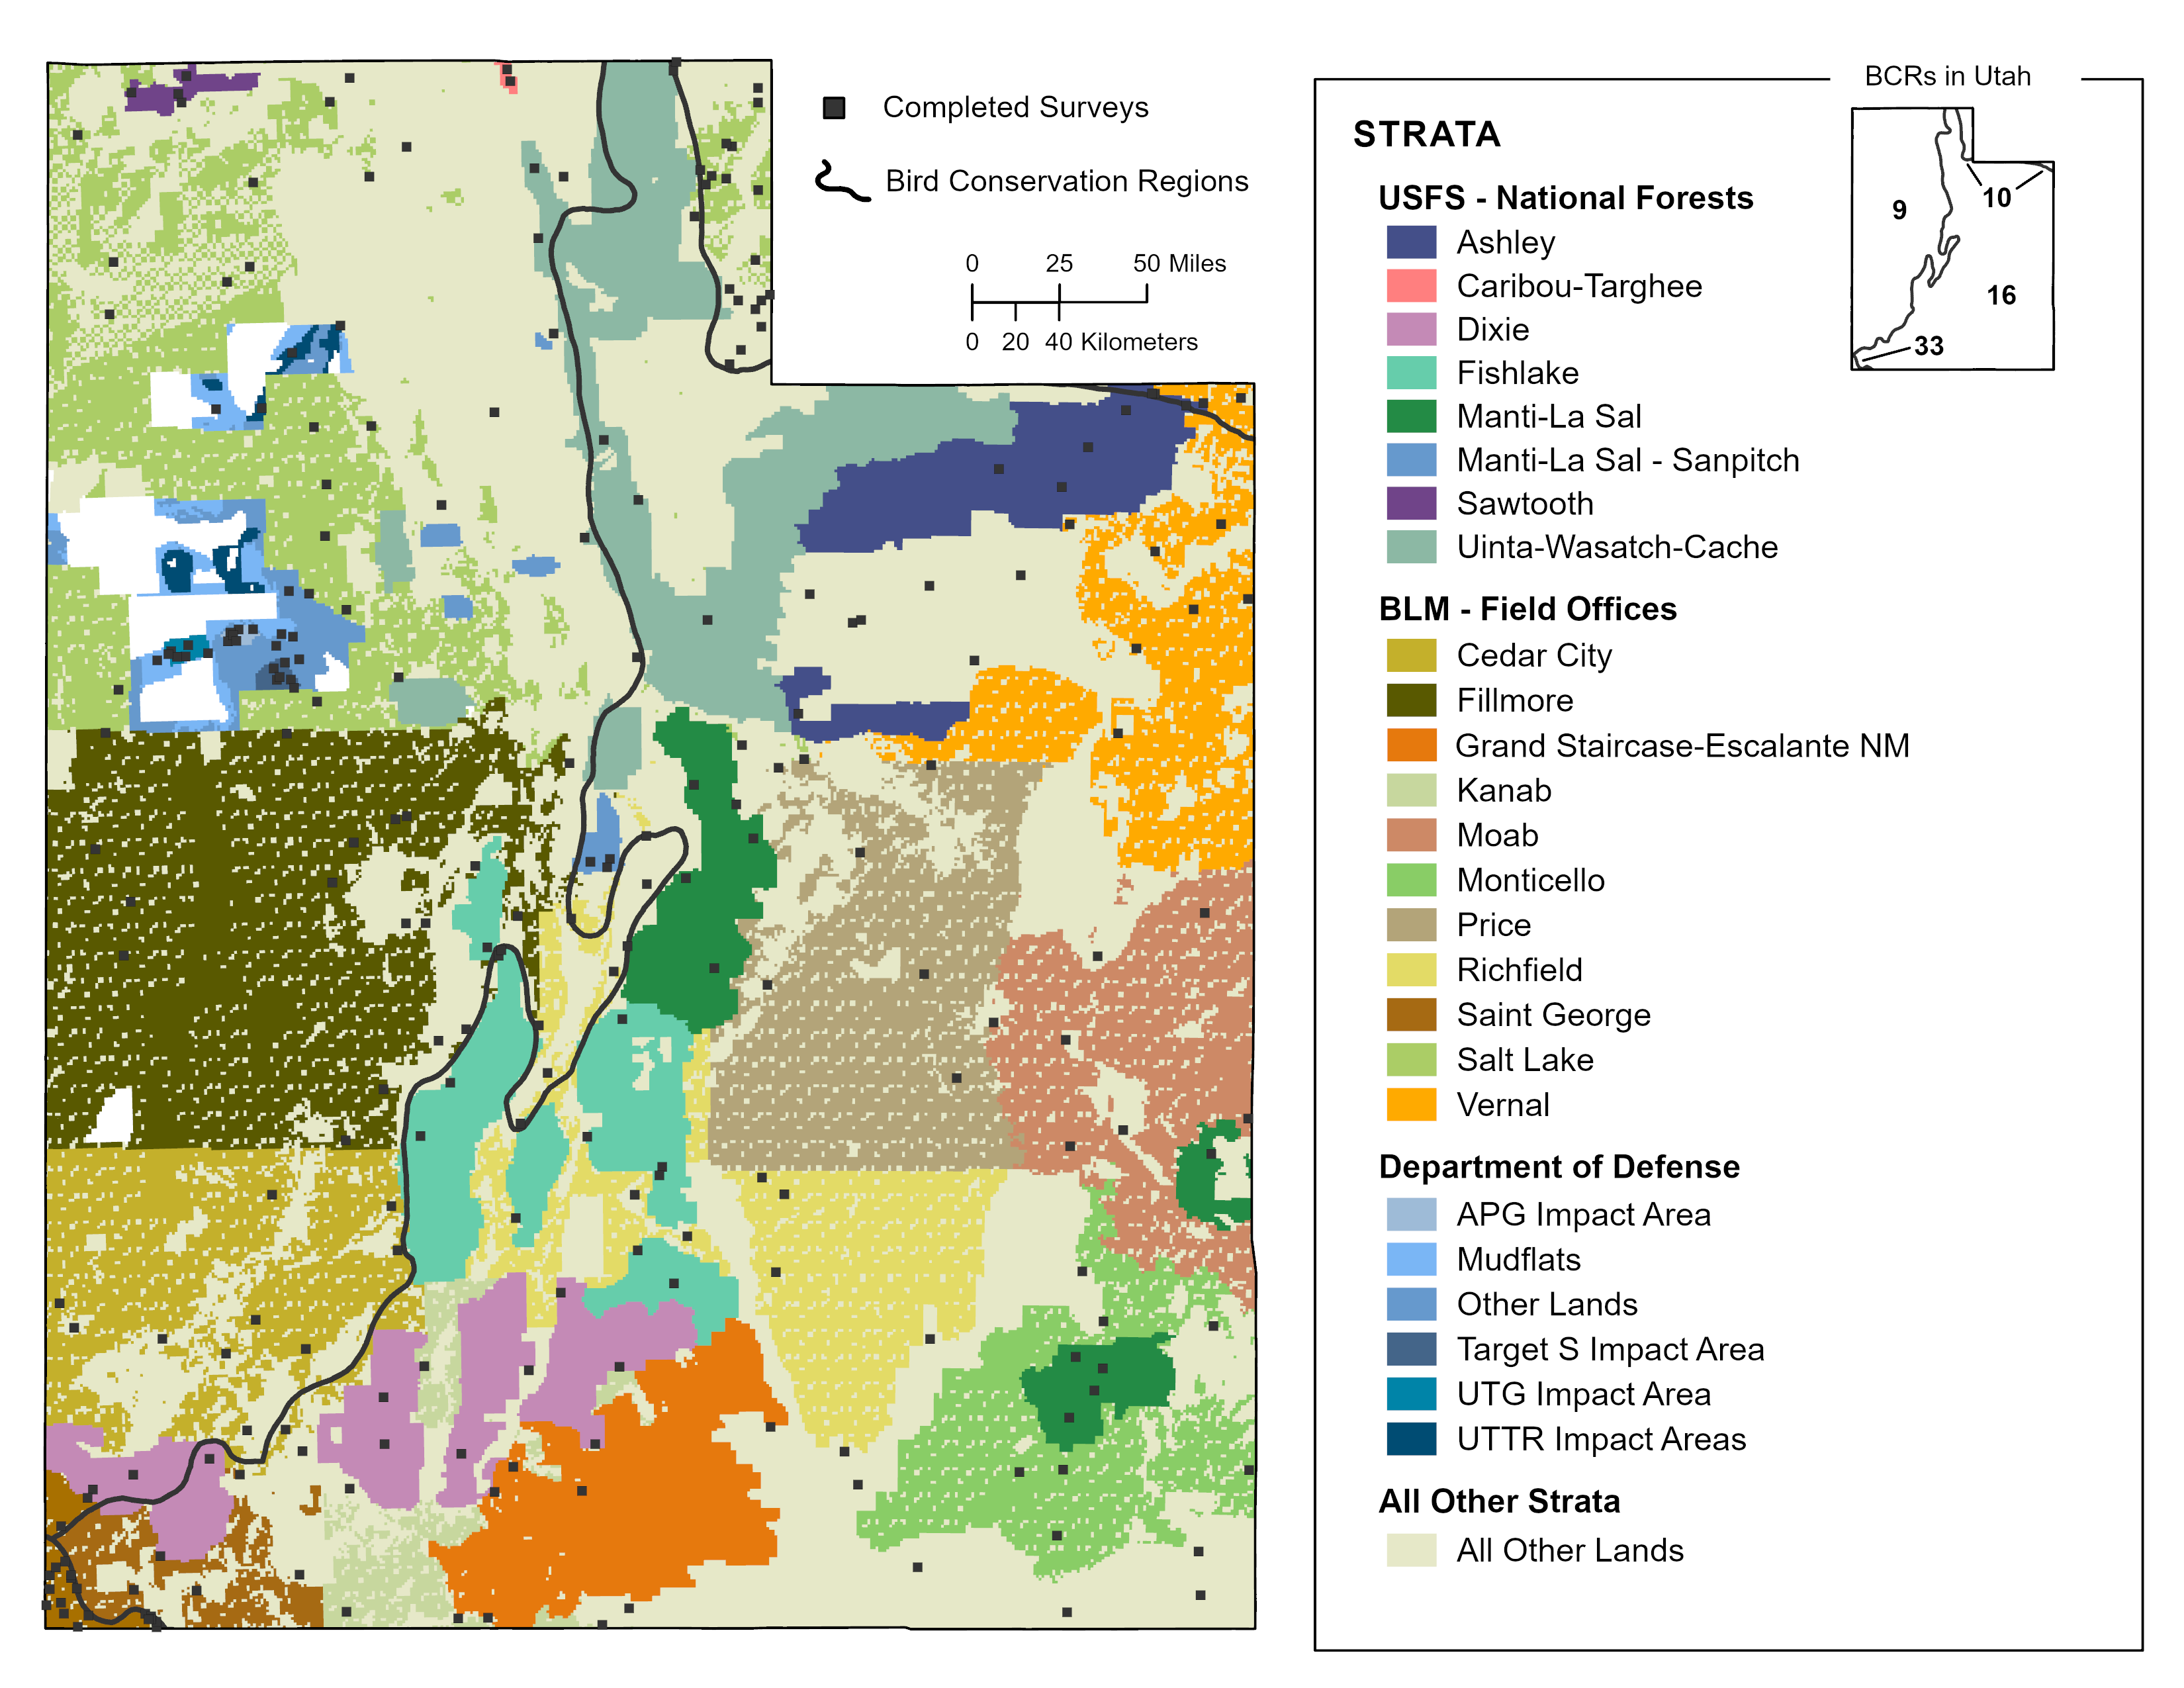
\includegraphics{./UT_Report_2022.png}

}

\caption{\label{fig-ut}Survey locations and strata in Utah, 2022.}

\end{figure}

\hypertarget{utah-statewide-total}{%
\subsubsection{Utah Statewide: Total}\label{utah-statewide-total}}

We obtained results for Utah Statewide: Total by compiling and jointly
analyzing data from 42 strata.

Field technicians completed 251 of 249 planned surveys (101\%) in 2022.
Technicians conducted 2815 point counts within the 249 surveyed grid
cells between May 2 and July 15. They detected 187 bird species,
including 13 priority species.

Bird Conservancy estimated densities and population sizes for 214
species that were detected in any year during which surveys were
conducted, 14 of which are priority species. The data yielded robust
density estimates (CV \textless{} 50\%) for 93 species.

Bird Conservancy estimated the proportion of 1 km² grid cells occupied
(Ψ, Psi) throughout Utah Statewide: Total for 220 species that were
detected in any year during which surveys were conducted, 15 of which
are priority species. The data yielded robust occupancy estimates (CV
\textless{} 50\%) for 135 species.

To view a map of survey locations, density and occupancy results and
species counts within Utah Statewide: Total across all years of the
project, follow the web link below. Hit ``Ok'' on the Rocky Mountain
Avian Data Center Disclaimer and hit the ``Run Query'' button
highlighted in red located near the top of the page (the map will zoom
to the area of interest). To view occupancy, density, or species counts
results, click on the respective tab in the upper left above the map.

\href{http://www.rmbo.org/new_site/adc/QueryWindow.aspx\#N4IgzgrgDgpgTmALnAhoiBbEAuABCAVQBUQBfIA=}{UT}

\hypertarget{all-other-lands-in-utah}{%
\subsubsection{All Other Lands in Utah}\label{all-other-lands-in-utah}}

We obtained results for All Other Lands in Utah by compiling and jointly
analyzing data from four strata.

Field technicians completed 110 of 111 planned surveys (99\%) in 2022.
Technicians conducted 1272 point counts within the 111 surveyed grid
cells between May 2 and July 13. They detected 161 bird species,
including 8 priority species.

Bird Conservancy estimated densities and population sizes for 192
species that were detected in any year during which surveys were
conducted, 12 of which are priority species. The data yielded robust
density estimates (CV \textless{} 50\%) for 85 species.

Bird Conservancy estimated the proportion of 1 km² grid cells occupied
(Ψ, Psi) throughout All Other Lands in Utah for 195 species that were
detected in any year during which surveys were conducted, 12 of which
are priority species. The data yielded robust occupancy estimates (CV
\textless{} 50\%) for 98 species.

To view a map of survey locations, density and occupancy results and
species counts within All Other Lands in Utah across all years of the
project, follow the web link below. Hit ``Ok'' on the Rocky Mountain
Avian Data Center Disclaimer and hit the ``Run Query'' button
highlighted in red located near the top of the page (the map will zoom
to the area of interest). To view occupancy, density, or species counts
results, click on the respective tab in the upper left above the map.

\href{http://www.rmbo.org/new_site/adc/QueryWindow.aspx\#N4IgzgrgDgpgTmALnAhoiBbEAuABCAVQBUBaAQQBsLcB5RAC3lwBkUA7AEzBAF8g}{UT-All
Other Lands}

\hypertarget{utah-bcr-9}{%
\section{Utah BCR 9}\label{utah-bcr-9}}

\hypertarget{utah-bcr-9-total}{%
\subsubsection{Utah BCR 9: Total}\label{utah-bcr-9-total}}

We obtained results for Utah BCR 9: Total by compiling and jointly
analyzing data from 17 strata.

Field technicians completed 101 of 99 planned surveys (102\%) in 2022.
Technicians conducted 1156 point counts within the 99 surveyed grid
cells between May 7 and July 14. They detected 120 bird species,
including 4 priority species.

Bird Conservancy estimated densities and population sizes for 160
species that were detected in any year during which surveys were
conducted, 10 of which are priority species. The data yielded robust
density estimates (CV \textless{} 50\%) for 57 species.

Bird Conservancy estimated the proportion of 1 km² grid cells occupied
(Ψ, Psi) throughout Utah BCR 9: Total for 168 species that were detected
in any year during which surveys were conducted, 14 of which are
priority species. The data yielded robust occupancy estimates (CV
\textless{} 50\%) for 84 species.

To view a map of survey locations, density and occupancy results and
species counts within Utah BCR 9: Total across all years of the project,
follow the web link below. Hit ``Ok'' on the Rocky Mountain Avian Data
Center Disclaimer and hit the ``Run Query'' button highlighted in red
located near the top of the page (the map will zoom to the area of
interest). To view occupancy, density, or species counts results, click
on the respective tab in the upper left above the map.

\href{http://www.rmbo.org/new_site/adc/QueryWindow.aspx\#N4IgzgrgDgpgTmALnAhoiBbEAuABCAVQBUBaAIQGEAlAThAF8g==}{UT-BCR9}

\hypertarget{all-other-lands-in-utah-bcr-9}{%
\subsubsection{All Other Lands in Utah BCR
9}\label{all-other-lands-in-utah-bcr-9}}

We obtained results for All Other Lands in Utah BCR 9 by compiling and
analyzing data from one stratum.

Field technicians completed 40 of 41 planned surveys (98\%) in 2022.
Technicians conducted 471 point counts within the 41 surveyed grid cells
between May 7 and June 28. They detected 85 bird species, including 2
priority species.

Bird Conservancy estimated densities and population sizes for 134
species that were detected in any year during which surveys were
conducted, 7 of which are priority species. The data yielded robust
density estimates (CV \textless{} 50\%) for 45 species.

Bird Conservancy estimated the proportion of 1 km² grid cells occupied
(Ψ, Psi) throughout All Other Lands in Utah BCR 9 for 132 species that
were detected in any year during which surveys were conducted, 7 of
which are priority species. The data yielded robust occupancy estimates
(CV \textless{} 50\%) for 51 species.

To view a map of survey locations, density and occupancy results and
species counts within All Other Lands in Utah BCR 9 across all years of
the project, follow the web link below. Hit ``Ok'' on the Rocky Mountain
Avian Data Center Disclaimer and hit the ``Run Query'' button
highlighted in red located near the top of the page (the map will zoom
to the area of interest). To view occupancy, density, or species counts
results, click on the respective tab in the upper left above the map.

\href{http://www.rmbo.org/new_site/adc/QueryWindow.aspx\#N4IgzgLgTghhCuBbEAuABCAqgFQLQCEBhAJQE5cBBAeXQoBs60qIALAUyjQBkYA7AEzAgAvkA===}{UT-BCR9-AO}

\hypertarget{utah-bcr-10}{%
\section{Utah BCR 10}\label{utah-bcr-10}}

\hypertarget{utah-bcr-10-total}{%
\subsubsection{Utah BCR 10: Total}\label{utah-bcr-10-total}}

We obtained results for Utah BCR 10: Total by compiling and jointly
analyzing data from five strata.

Field technicians completed 26 of 25 planned surveys (104\%) in 2022.
Technicians conducted 260 point counts within the 25 surveyed grid cells
between May 21 and July 14. They detected 84 bird species, including 4
priority species.

Bird Conservancy estimated densities and population sizes for 130
species that were detected in any year during which surveys were
conducted, 6 of which are priority species. The data yielded robust
density estimates (CV \textless{} 50\%) for 41 species.

Bird Conservancy estimated the proportion of 1 km² grid cells occupied
(Ψ, Psi) throughout Utah BCR 10: Total for 128 species that were
detected in any year during which surveys were conducted, 6 of which are
priority species. The data yielded robust occupancy estimates (CV
\textless{} 50\%) for 51 species.

To view a map of survey locations, density and occupancy results and
species counts within Utah BCR 10: Total across all years of the
project, follow the web link below. Hit ``Ok'' on the Rocky Mountain
Avian Data Center Disclaimer and hit the ``Run Query'' button
highlighted in red located near the top of the page (the map will zoom
to the area of interest). To view occupancy, density, or species counts
results, click on the respective tab in the upper left above the map.

\href{http://www.rmbo.org/new_site/adc/QueryWindow.aspx\#N4IgzgrgDgpgTmALnAhoiBbEAuABCAVQBUBaAIQGEAlARgAYQBfIA===}{UT-BCR10}

\hypertarget{all-other-lands-in-utah-bcr-10}{%
\subsubsection{All Other Lands in Utah BCR
10}\label{all-other-lands-in-utah-bcr-10}}

We obtained results for All Other Lands in Utah BCR 10 by compiling and
analyzing data from one stratum.

Field technicians completed 15 of 14 planned surveys (107\%) in 2022.
Technicians conducted 158 point counts within the 14 surveyed grid cells
between May 21 and June 27. They detected 45 bird species, including 4
priority species.

Bird Conservancy estimated densities and population sizes for 91 species
that were detected in any year during which surveys were conducted, 4 of
which are priority species. The data yielded robust density estimates
(CV \textless{} 50\%) for 16 species.

Bird Conservancy estimated the proportion of 1 km² grid cells occupied
(Ψ, Psi) throughout All Other Lands in Utah BCR 10 for 87 species that
were detected in any year during which surveys were conducted, 4 of
which are priority species. The data yielded robust occupancy estimates
(CV \textless{} 50\%) for 28 species.

To view a map of survey locations, density and occupancy results and
species counts within All Other Lands in Utah BCR 10 across all years of
the project, follow the web link below. Hit ``Ok'' on the Rocky Mountain
Avian Data Center Disclaimer and hit the ``Run Query'' button
highlighted in red located near the top of the page (the map will zoom
to the area of interest). To view occupancy, density, or species counts
results, click on the respective tab in the upper left above the map.

\href{http://www.rmbo.org/new_site/adc/QueryWindow.aspx\#N4IgzgLgTghhCuBbEAuABCAqgFQLQCEBhAJQEYAGXAQQHl0qAbBtGiACwFMo0AZGAOwAmYEAF8gA}{UT-BCR10-AO}

\hypertarget{utah-bcr-16}{%
\section{Utah BCR 16}\label{utah-bcr-16}}

\hypertarget{utah-bcr-16-total}{%
\subsubsection{Utah BCR 16: Total}\label{utah-bcr-16-total}}

We obtained results for Utah BCR 16: Total by compiling and jointly
analyzing data from 18 strata.

Field technicians completed 107 of 108 planned surveys (99\%) in 2022.
Technicians conducted 1191 point counts within the 108 surveyed grid
cells between May 7 and July 15. They detected 146 bird species,
including 6 priority species.

Bird Conservancy estimated densities and population sizes for 188
species that were detected in any year during which surveys were
conducted, 9 of which are priority species. The data yielded robust
density estimates (CV \textless{} 50\%) for 81 species.

Bird Conservancy estimated the proportion of 1 km² grid cells occupied
(Ψ, Psi) throughout Utah BCR 16: Total for 185 species that were
detected in any year during which surveys were conducted, 9 of which are
priority species. The data yielded robust occupancy estimates (CV
\textless{} 50\%) for 116 species.

To view a map of survey locations, density and occupancy results and
species counts within Utah BCR 16: Total across all years of the
project, follow the web link below. Hit ``Ok'' on the Rocky Mountain
Avian Data Center Disclaimer and hit the ``Run Query'' button
highlighted in red located near the top of the page (the map will zoom
to the area of interest). To view occupancy, density, or species counts
results, click on the respective tab in the upper left above the map.

\href{http://www.rmbo.org/new_site/adc/QueryWindow.aspx\#N4IgzgrgDgpgTmALnAhoiBbEAuABCAVQBUBaAIQGEAlARgDYQBfIA===}{UT-BCR16}

\hypertarget{all-other-lands-in-utah-bcr-16}{%
\subsubsection{All Other Lands in Utah BCR
16}\label{all-other-lands-in-utah-bcr-16}}

We obtained results for All Other Lands in Utah BCR 16 by compiling and
analyzing data from one stratum.

Field technicians completed 40 of 41 planned surveys (98\%) in 2022.
Technicians conducted 461 point counts within the 41 surveyed grid cells
between May 10 and July 13. They detected 112 bird species, including 3
priority species.

Bird Conservancy estimated densities and population sizes for 159
species that were detected in any year during which surveys were
conducted, 8 of which are priority species. The data yielded robust
density estimates (CV \textless{} 50\%) for 72 species.

Bird Conservancy estimated the proportion of 1 km² grid cells occupied
(Ψ, Psi) throughout All Other Lands in Utah BCR 16 for 156 species that
were detected in any year during which surveys were conducted, 8 of
which are priority species. The data yielded robust occupancy estimates
(CV \textless{} 50\%) for 67 species.

To view a map of survey locations, density and occupancy results and
species counts within All Other Lands in Utah BCR 16 across all years of
the project, follow the web link below. Hit ``Ok'' on the Rocky Mountain
Avian Data Center Disclaimer and hit the ``Run Query'' button
highlighted in red located near the top of the page (the map will zoom
to the area of interest). To view occupancy, density, or species counts
results, click on the respective tab in the upper left above the map.

\href{http://www.rmbo.org/new_site/adc/QueryWindow.aspx\#N4IgzgLgTghhCuBbEAuABCAqgFQLQCEBhAJQEYA2XAQQHl0qAbBtGiACwFMo0AZGAOwAmYEAF8gA}{UT-BCR16-AO}

\hypertarget{utah-bcr-33}{%
\section{Utah BCR 33}\label{utah-bcr-33}}

\hypertarget{utah-bcr-33-total}{%
\subsubsection{Utah BCR 33: Total}\label{utah-bcr-33-total}}

We obtained results for Utah BCR 33: Total by compiling and jointly
analyzing data from two strata.

Field technicians completed all planned surveys (100\%) in 2022.
Technicians conducted 208 point counts within the 17 surveyed grid cells
between May 2 and May 21. They detected 101 bird species, including 3
priority species.

Bird Conservancy estimated densities and population sizes for 112
species that were detected in any year during which surveys were
conducted, 3 of which are priority species. The data yielded robust
density estimates (CV \textless{} 50\%) for 24 species.

Bird Conservancy estimated the proportion of 1 km² grid cells occupied
(Ψ, Psi) throughout Utah BCR 33: Total for 114 species that were
detected in any year during which surveys were conducted, 3 of which are
priority species. The data yielded robust occupancy estimates (CV
\textless{} 50\%) for 28 species.

To view a map of survey locations, density and occupancy results and
species counts within Utah BCR 33: Total across all years of the
project, follow the web link below. Hit ``Ok'' on the Rocky Mountain
Avian Data Center Disclaimer and hit the ``Run Query'' button
highlighted in red located near the top of the page (the map will zoom
to the area of interest). To view occupancy, density, or species counts
results, click on the respective tab in the upper left above the map.

\href{http://www.rmbo.org/new_site/adc/QueryWindow.aspx\#N4IgzgrgDgpgTmALnAhoiBbEAuABCAVQBUBaAIQGEAlAZhpAF8g=}{UT-BCR33}

\hypertarget{all-other-lands-in-utah-bcr-33}{%
\subsubsection{All Other Lands in Utah BCR
33}\label{all-other-lands-in-utah-bcr-33}}

We obtained results for All Other Lands in Utah BCR 33 by compiling and
analyzing data from one stratum.

Field technicians completed all planned surveys (100\%) in 2022.
Technicians conducted 182 point counts within the 15 surveyed grid cells
between May 2 and May 21. They detected 95 bird species, including 2
priority species.

Bird Conservancy estimated densities and population sizes for 105
species that were detected in any year during which surveys were
conducted, 1 of which are priority species. The data yielded robust
density estimates (CV \textless{} 50\%) for 31 species.

Bird Conservancy estimated the proportion of 1 km² grid cells occupied
(Ψ, Psi) throughout All Other Lands in Utah BCR 33 for 106 species that
were detected in any year during which surveys were conducted, 1 of
which are priority species. The data yielded robust occupancy estimates
(CV \textless{} 50\%) for 33 species.

To view a map of survey locations, density and occupancy results and
species counts within All Other Lands in Utah BCR 33 across all years of
the project, follow the web link below. Hit ``Ok'' on the Rocky Mountain
Avian Data Center Disclaimer and hit the ``Run Query'' button
highlighted in red located near the top of the page (the map will zoom
to the area of interest). To view occupancy, density, or species counts
results, click on the respective tab in the upper left above the map.

\href{http://www.rmbo.org/new_site/adc/QueryWindow.aspx\#N4IgzgLgTghhCuBbEAuABCAqgFQLQCEBhAJQGZTcBBAeXUoBt61qIALAUyjQBkYA7ACZgQAXyA==}{UT-BCR33-AO}

\hypertarget{wyoming}{%
\chapter{Wyoming}\label{wyoming}}

\begin{figure}

{\centering 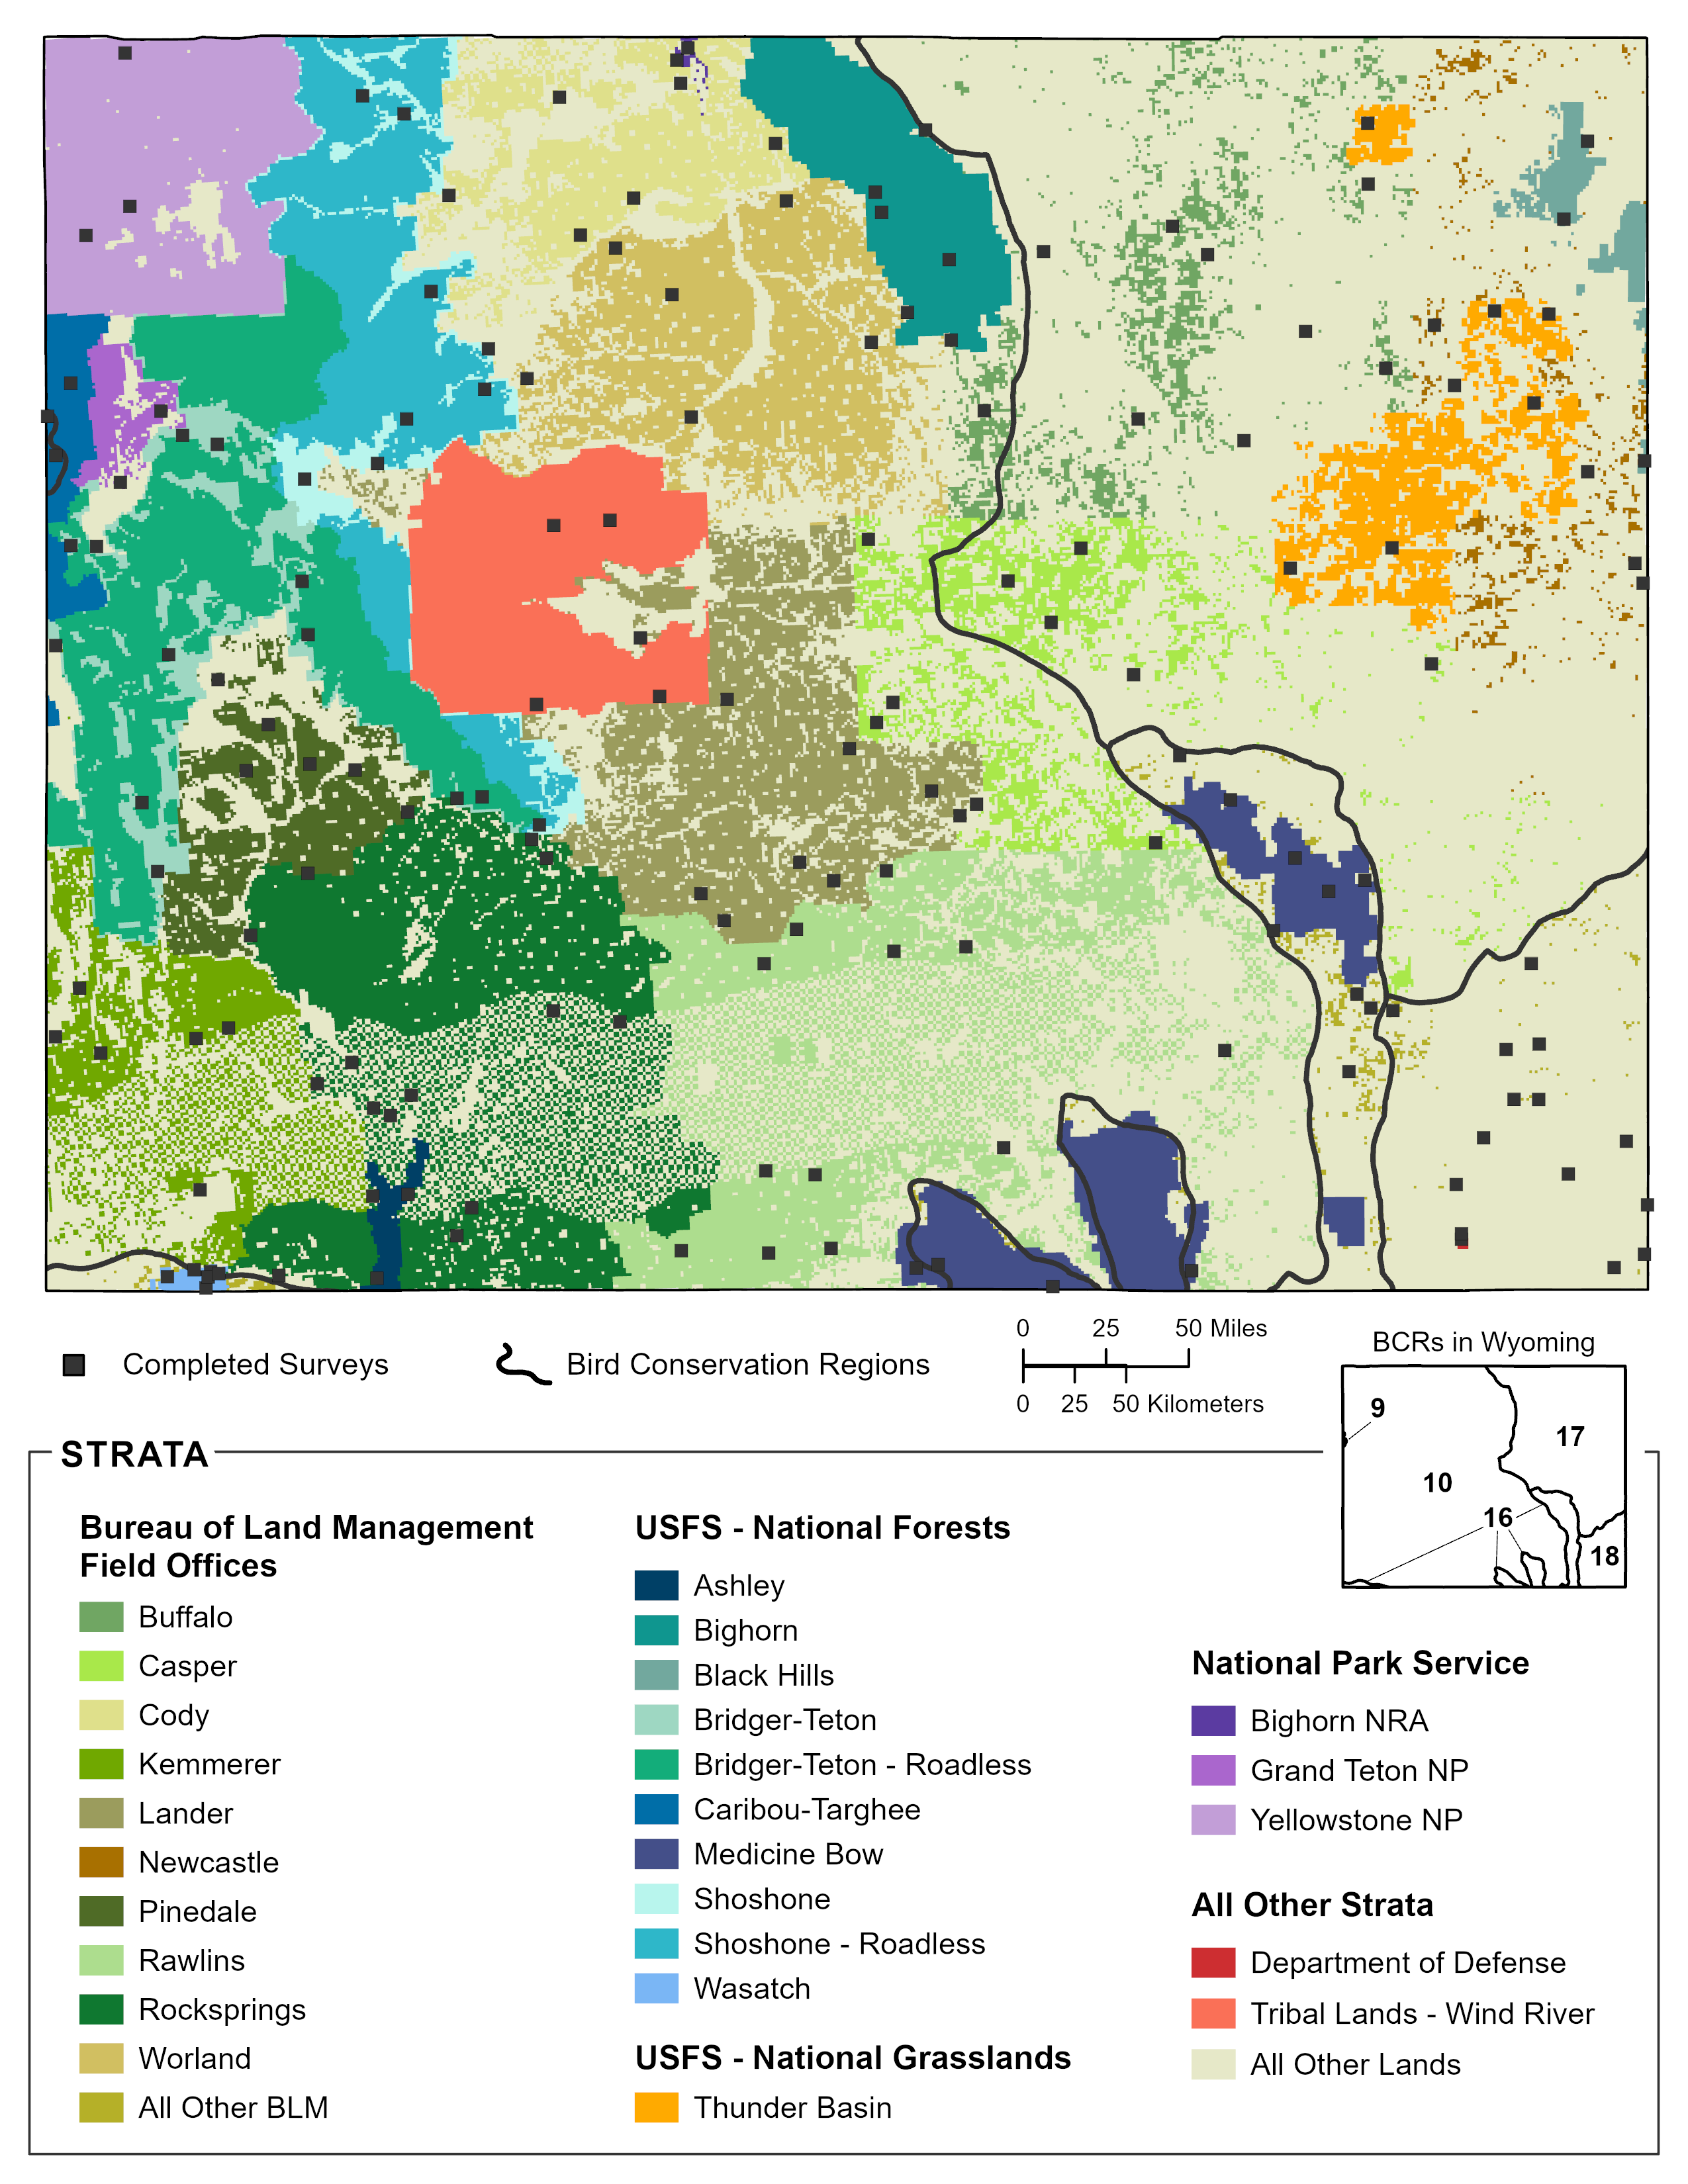
\includegraphics{./WY_Report_2022.png}

}

\caption{\label{fig-wy}Survey locations and strata in Wyoming, 2022.}

\end{figure}

\hypertarget{wyoming-statewide-total}{%
\subsubsection{Wyoming Statewide: Total}\label{wyoming-statewide-total}}

We obtained results for Wyoming Statewide: Total by compiling and
jointly analyzing data from 37 strata.

Field technicians completed 173 of 170 planned surveys (102\%) in 2022.
Technicians conducted 2173 point counts within the 170 surveyed grid
cells between May 24 and July 20. They detected 190 bird species,
including 44 priority species.

Bird Conservancy estimated densities and population sizes for 217
species that were detected in any year during which surveys were
conducted, 61 of which are priority species. The data yielded robust
density estimates (CV \textless{} 50\%) for 94 species.

Bird Conservancy estimated the proportion of 1 km² grid cells occupied
(Ψ, Psi) throughout Wyoming Statewide: Total for 222 species that were
detected in any year during which surveys were conducted, 61 of which
are priority species. The data yielded robust occupancy estimates (CV
\textless{} 50\%) for 143 species.

To view a map of survey locations, density and occupancy results and
species counts within Wyoming Statewide: Total across all years of the
project, follow the web link below. Hit ``Ok'' on the Rocky Mountain
Avian Data Center Disclaimer and hit the ``Run Query'' button
highlighted in red located near the top of the page (the map will zoom
to the area of interest). To view occupancy, density, or species counts
results, click on the respective tab in the upper left above the map.

\href{http://www.rmbo.org/new_site/adc/QueryWindow.aspx\#N4IgzgrgDgpgTmALnAhoiBbEAuABCAdQE0QBfIA=}{WY}

\hypertarget{all-other-lands-in-wyoming}{%
\subsubsection{All Other Lands in
Wyoming}\label{all-other-lands-in-wyoming}}

We obtained results for All Other Lands in Wyoming by compiling and
jointly analyzing data from four strata.

Field technicians completed 44 of 42 planned surveys (105\%) in 2022.
Technicians conducted 464 point counts within the 42 surveyed grid cells
between May 24 and June 24. They detected 141 bird species, including 28
priority species.

Bird Conservancy estimated densities and population sizes for 192
species that were detected in any year during which surveys were
conducted, 50 of which are priority species. The data yielded robust
density estimates (CV \textless{} 50\%) for 57 species.

Bird Conservancy estimated the proportion of 1 km² grid cells occupied
(Ψ, Psi) throughout All Other Lands in Wyoming for 192 species that were
detected in any year during which surveys were conducted, 50 of which
are priority species. The data yielded robust occupancy estimates (CV
\textless{} 50\%) for 88 species.

To view a map of survey locations, density and occupancy results and
species counts within All Other Lands in Wyoming across all years of the
project, follow the web link below. Hit ``Ok'' on the Rocky Mountain
Avian Data Center Disclaimer and hit the ``Run Query'' button
highlighted in red located near the top of the page (the map will zoom
to the area of interest). To view occupancy, density, or species counts
results, click on the respective tab in the upper left above the map.

\href{http://www.rmbo.org/new_site/adc/QueryWindow.aspx\#N4IgzgrgDgpgTmALnAhoiBbEAuABCAdQE0BaAQQBsLcB5RAC3hAF8g==}{WY-All
Other}

\hypertarget{wyoming-bcr-10}{%
\section{Wyoming BCR 10}\label{wyoming-bcr-10}}

\hypertarget{wyoming-bcr-10-total}{%
\subsubsection{Wyoming BCR 10: Total}\label{wyoming-bcr-10-total}}

We obtained results for Wyoming BCR 10: Total by compiling and jointly
analyzing data from 23 strata.

Field technicians completed 112 of 111 planned surveys (101\%) in 2022.
Technicians conducted 1470 point counts within the 111 surveyed grid
cells between May 24 and July 20. They detected 171 bird species,
including 40 priority species.

Bird Conservancy estimated densities and population sizes for 201
species that were detected in any year during which surveys were
conducted, 55 of which are priority species. The data yielded robust
density estimates (CV \textless{} 50\%) for 83 species.

Bird Conservancy estimated the proportion of 1 km² grid cells occupied
(Ψ, Psi) throughout Wyoming BCR 10: Total for 203 species that were
detected in any year during which surveys were conducted, 54 of which
are priority species. The data yielded robust occupancy estimates (CV
\textless{} 50\%) for 123 species.

To view a map of survey locations, density and occupancy results and
species counts within Wyoming BCR 10: Total across all years of the
project, follow the web link below. Hit ``Ok'' on the Rocky Mountain
Avian Data Center Disclaimer and hit the ``Run Query'' button
highlighted in red located near the top of the page (the map will zoom
to the area of interest). To view occupancy, density, or species counts
results, click on the respective tab in the upper left above the map.

\href{http://www.rmbo.org/new_site/adc/QueryWindow.aspx\#N4IgzgrgDgpgTmALnAhoiBbEAuABCAdQE0BaAIQGEAlARgAYQBfIA===}{WY-BCR10}

\hypertarget{all-other-lands-in-wyoming-bcr-10}{%
\subsubsection{All Other Lands in Wyoming BCR
10}\label{all-other-lands-in-wyoming-bcr-10}}

We obtained results for All Other Lands in Wyoming BCR 10 by compiling
and analyzing data from one stratum.

Field technicians completed all planned surveys (100\%) in 2022.
Technicians conducted 158 point counts within the 15 surveyed grid cells
between May 25 and June 24. They detected 107 bird species, including 22
priority species.

Bird Conservancy estimated densities and population sizes for 164
species that were detected in any year during which surveys were
conducted, 36 of which are priority species. The data yielded robust
density estimates (CV \textless{} 50\%) for 40 species.

Bird Conservancy estimated the proportion of 1 km² grid cells occupied
(Ψ, Psi) throughout All Other Lands in Wyoming BCR 10 for 161 species
that were detected in any year during which surveys were conducted, 36
of which are priority species. The data yielded robust occupancy
estimates (CV \textless{} 50\%) for 56 species.

To view a map of survey locations, density and occupancy results and
species counts within All Other Lands in Wyoming BCR 10 across all years
of the project, follow the web link below. Hit ``Ok'' on the Rocky
Mountain Avian Data Center Disclaimer and hit the ``Run Query'' button
highlighted in red located near the top of the page (the map will zoom
to the area of interest). To view occupancy, density, or species counts
results, click on the respective tab in the upper left above the map.

\href{http://www.rmbo.org/new_site/adc/QueryWindow.aspx\#N4IgzgLgTghhCuBbEAuABCA6gTQLQCEBhAJQEYAGXAQQHl0qAbBtGiACwFMo0AZGAOwAmYEAF8gA}{WY-BCR10-AO}

\hypertarget{wyoming-bcr-16}{%
\section{Wyoming BCR 16}\label{wyoming-bcr-16}}

\hypertarget{wyoming-bcr-16-total}{%
\subsubsection{Wyoming BCR 16: Total}\label{wyoming-bcr-16-total}}

We obtained results for Wyoming BCR 16: Total by compiling and jointly
analyzing data from four strata.

Field technicians completed all planned surveys (100\%) in 2022.
Technicians conducted 150 point counts within the 14 surveyed grid cells
between June 4 and July 15. They detected 89 bird species, including 13
priority species.

Bird Conservancy estimated densities and population sizes for 164
species that were detected in any year during which surveys were
conducted, 37 of which are priority species. The data yielded robust
density estimates (CV \textless{} 50\%) for 36 species.

Bird Conservancy estimated the proportion of 1 km² grid cells occupied
(Ψ, Psi) throughout Wyoming BCR 16: Total for 159 species that were
detected in any year during which surveys were conducted, 36 of which
are priority species. The data yielded robust occupancy estimates (CV
\textless{} 50\%) for 65 species.

To view a map of survey locations, density and occupancy results and
species counts within Wyoming BCR 16: Total across all years of the
project, follow the web link below. Hit ``Ok'' on the Rocky Mountain
Avian Data Center Disclaimer and hit the ``Run Query'' button
highlighted in red located near the top of the page (the map will zoom
to the area of interest). To view occupancy, density, or species counts
results, click on the respective tab in the upper left above the map.

\href{http://www.rmbo.org/new_site/adc/QueryWindow.aspx\#N4IgzgrgDgpgTmALnAhoiBbEAuABCAdQE0BaAIQGEAlARgDYQBfIA===}{WY-BCR16}

\hypertarget{all-other-lands-in-wyoming-bcr-16}{%
\subsubsection{All Other Lands in Wyoming BCR
16}\label{all-other-lands-in-wyoming-bcr-16}}

We obtained results for All Other Lands in Wyoming BCR 16 by compiling
and analyzing data from one stratum.

Field technicians completed all planned surveys (100\%) in 2022.
Technicians conducted 42 point counts within the 5 surveyed grid cells
between June 7 and June 23. They detected 52 bird species, including 9
priority species.

Bird Conservancy estimated densities and population sizes for 114
species that were detected in any year during which surveys were
conducted, 22 of which are priority species. The data yielded robust
density estimates (CV \textless{} 50\%) for 14 species.

Bird Conservancy estimated the proportion of 1 km² grid cells occupied
(Ψ, Psi) throughout All Other Lands in Wyoming BCR 16 for 107 species
that were detected in any year during which surveys were conducted, 21
of which are priority species. The data yielded robust occupancy
estimates (CV \textless{} 50\%) for 22 species.

To view a map of survey locations, density and occupancy results and
species counts within All Other Lands in Wyoming BCR 16 across all years
of the project, follow the web link below. Hit ``Ok'' on the Rocky
Mountain Avian Data Center Disclaimer and hit the ``Run Query'' button
highlighted in red located near the top of the page (the map will zoom
to the area of interest). To view occupancy, density, or species counts
results, click on the respective tab in the upper left above the map.

\href{http://www.rmbo.org/new_site/adc/QueryWindow.aspx\#N4IgzgLgTghhCuBbEAuABCA6gTQLQCEBhAJQEYA2XAQQHl0qAbBtGiACwFMo0AZGAOwAmYEAF8gA}{WY-BCR16-AO}

\hypertarget{wyoming-bcr-17}{%
\section{Wyoming BCR 17}\label{wyoming-bcr-17}}

\hypertarget{wyoming-bcr-17-total}{%
\subsubsection{Wyoming BCR 17: Total}\label{wyoming-bcr-17-total}}

We obtained results for Wyoming BCR 17: Total by compiling and jointly
analyzing data from six strata.

Field technicians completed 29 of 28 planned surveys (104\%) in 2022.
Technicians conducted 357 point counts within the 28 surveyed grid cells
between May 24 and June 22. They detected 110 bird species, including 23
priority species.

Bird Conservancy estimated densities and population sizes for 175
species that were detected in any year during which surveys were
conducted, 43 of which are priority species. The data yielded robust
density estimates (CV \textless{} 50\%) for 41 species.

Bird Conservancy estimated the proportion of 1 km² grid cells occupied
(Ψ, Psi) throughout Wyoming BCR 17: Total for 176 species that were
detected in any year during which surveys were conducted, 42 of which
are priority species. The data yielded robust occupancy estimates (CV
\textless{} 50\%) for 58 species.

To view a map of survey locations, density and occupancy results and
species counts within Wyoming BCR 17: Total across all years of the
project, follow the web link below. Hit ``Ok'' on the Rocky Mountain
Avian Data Center Disclaimer and hit the ``Run Query'' button
highlighted in red located near the top of the page (the map will zoom
to the area of interest). To view occupancy, density, or species counts
results, click on the respective tab in the upper left above the map.

\href{http://www.rmbo.org/new_site/adc/QueryWindow.aspx\#N4IgzgrgDgpgTmALnAhoiBbEAuABCAdQE0BaAIQGEAlARgHYQBfIA===}{WY-BCR17}

\hypertarget{all-other-lands-in-wyoming-bcr-17}{%
\subsubsection{All Other Lands in Wyoming BCR
17}\label{all-other-lands-in-wyoming-bcr-17}}

We obtained results for All Other Lands in Wyoming BCR 17 by compiling
and analyzing data from one stratum.

Field technicians completed 12 of 11 planned surveys (109\%) in 2022.
Technicians conducted 132 point counts within the 11 surveyed grid cells
between May 24 and June 16. They detected 90 bird species, including 20
priority species.

Bird Conservancy estimated densities and population sizes for 145
species that were detected in any year during which surveys were
conducted, 31 of which are priority species. The data yielded robust
density estimates (CV \textless{} 50\%) for 33 species.

Bird Conservancy estimated the proportion of 1 km² grid cells occupied
(Ψ, Psi) throughout All Other Lands in Wyoming BCR 17 for 141 species
that were detected in any year during which surveys were conducted, 28
of which are priority species. The data yielded robust occupancy
estimates (CV \textless{} 50\%) for 45 species.

To view a map of survey locations, density and occupancy results and
species counts within All Other Lands in Wyoming BCR 17 across all years
of the project, follow the web link below. Hit ``Ok'' on the Rocky
Mountain Avian Data Center Disclaimer and hit the ``Run Query'' button
highlighted in red located near the top of the page (the map will zoom
to the area of interest). To view occupancy, density, or species counts
results, click on the respective tab in the upper left above the map.

\href{http://www.rmbo.org/new_site/adc/QueryWindow.aspx\#N4IgzgLgTghhCuBbEAuABCA6gTQLQCEBhAJQEYB2XAQQHl0qAbBtGiACwFMo0AZGAOwAmYEAF8gA}{WY-BCR17-AO}

\hypertarget{wyoming-bcr-18}{%
\section{Wyoming BCR 18}\label{wyoming-bcr-18}}

\hypertarget{wyoming-bcr-18-total}{%
\subsubsection{Wyoming BCR 18: Total}\label{wyoming-bcr-18-total}}

We obtained results for Wyoming BCR 18: Total by compiling and jointly
analyzing data from three strata.

Field technicians completed 16 of 15 planned surveys (107\%) in 2022.
Technicians conducted 176 point counts within the 15 surveyed grid cells
between May 25 and June 16. They detected 63 bird species, including 12
priority species.

Bird Conservancy estimated densities and population sizes for 111
species that were detected in any year during which surveys were
conducted, 28 of which are priority species. The data yielded robust
density estimates (CV \textless{} 50\%) for 21 species.

Bird Conservancy estimated the proportion of 1 km² grid cells occupied
(Ψ, Psi) throughout Wyoming BCR 18: Total for 109 species that were
detected in any year during which surveys were conducted, 27 of which
are priority species. The data yielded robust occupancy estimates (CV
\textless{} 50\%) for 30 species.

To view a map of survey locations, density and occupancy results and
species counts within Wyoming BCR 18: Total across all years of the
project, follow the web link below. Hit ``Ok'' on the Rocky Mountain
Avian Data Center Disclaimer and hit the ``Run Query'' button
highlighted in red located near the top of the page (the map will zoom
to the area of interest). To view occupancy, density, or species counts
results, click on the respective tab in the upper left above the map.

\href{http://www.rmbo.org/new_site/adc/QueryWindow.aspx\#N4IgzgrgDgpgTmALnAhoiBbEAuABCAdQE0BaAIQGEAlARgA4QBfIA===}{WY-BCR18}

\hypertarget{all-other-lands-in-wyoming-bcr-18}{%
\subsubsection{All Other Lands in Wyoming BCR
18}\label{all-other-lands-in-wyoming-bcr-18}}

We obtained results for All Other Lands in Wyoming BCR 18 by compiling
and analyzing data from one stratum.

Field technicians completed 12 of 11 planned surveys (109\%) in 2022.
Technicians conducted 132 point counts within the 11 surveyed grid cells
between May 31 and June 16. They detected 54 bird species, including 17
priority species.

Bird Conservancy estimated densities and population sizes for 104
species that were detected in any year during which surveys were
conducted, 25 of which are priority species. The data yielded robust
density estimates (CV \textless{} 50\%) for 21 species.

Bird Conservancy estimated the proportion of 1 km² grid cells occupied
(Ψ, Psi) throughout All Other Lands in Wyoming BCR 18 for 100 species
that were detected in any year during which surveys were conducted, 24
of which are priority species. The data yielded robust occupancy
estimates (CV \textless{} 50\%) for 29 species.

To view a map of survey locations, density and occupancy results and
species counts within All Other Lands in Wyoming BCR 18 across all years
of the project, follow the web link below. Hit ``Ok'' on the Rocky
Mountain Avian Data Center Disclaimer and hit the ``Run Query'' button
highlighted in red located near the top of the page (the map will zoom
to the area of interest). To view occupancy, density, or species counts
results, click on the respective tab in the upper left above the map.

\href{http://www.rmbo.org/new_site/adc/QueryWindow.aspx\#N4IgzgLgTghhCuBbEAuABCA6gTQLQCEBhAJQEYAOXAQQHl0qAbBtGiACwFMo0AZGAOwAmYEAF8gA}{WY-BCR18-AO}

\part{Discussion}

\hypertarget{data-applications}{%
\chapter{Data Applications}\label{data-applications}}

Each year, we collected breeding bird information in the Great Plains,
Rocky Mountains, and Intermountain West and estimated occupancy,
density, abundance, and population trend at a variety of spatial scales.
This information is used in a variety of ways by IMBCR partners to
inform avian conservation and management decisions, such as:

\begin{quote}
\textbf{State wildlife agencies} use the trend estimates to monitor
Species of Greatest Conservation Need and revise their State Wildlife
Action Plans. Trend estimates allow them to identify species that may
need additional conservation efforts (e.g., declining populations) or
species-specific monitoring efforts. Conversely, species with increasing
populations across a state may warrant a lower priority status.
\end{quote}

\hypertarget{federal-agency-partners}{%
\subsubsection{Federal agency partners}\label{federal-agency-partners}}

\begin{quote}
The \textbf{Bureau of Land Management} (BLM) use the density estimates
for project-level planning in specific strata, such as a field office.
The density estimates inform potential population impacts on species of
concern for NEPA projects and environmental assessments by multiplying
the densities by the project area to determine the potential number of
individuals that could be impacted by the project.

The \textbf{U.S. Forest Service} (USFS) uses the trend estimates to
monitor focal species within a unit's Land Management Plan, and to
support larger processes under forest plan revision, such as assessing
species of conservation concern and identifying focal species.

The \textbf{Department of Defens}e (DoD) uses the density and trend
estimates for priority species to examine impacts of installation
activities on birds. They also compare estimates for specific DoD strata
to surrounding regional estimates for context.
\end{quote}

\hypertarget{recent-overlay-projects}{%
\section{Recent Overlay Projects}\label{recent-overlay-projects}}

IMBCR partners also implement overlays, or targeted projects, to address
specific management questions. Overlay projects use the same sampling
design and field methods but are not integrated into the nested
stratification of the IMBCR program. These projects benefit from pooling
detection data across the IMBCR program, and have regional context for
project-specific estimates. Some overlay projects include:

\begin{quote}
Monitored birds in the Atlantic Rim Natural Gas area (south-central
Wyoming) to \textbf{determine energy development impacts on birds}, and
set management triggers to determine when a threshold is met for
sagebrush songbird occupancy in the project area compared to surrounding
BLM lands.
\end{quote}

\begin{quote}
Examined community-level effects and bird species relationships with
restoration treatments under the \textbf{USFS's Collaborative Forest
Landscape Restoration Program} implemented across the Front Range in
Colorado.
\end{quote}

\begin{quote}
Compared population estimates on private ranches in the Great Plains to
estimates in the surrounding region to see if ranches participating in
the \textbf{Audubon Conservation Ranching} program provide breeding
habitat for grassland birds.
\end{quote}

\hypertarget{adaptive-management}{%
\section{Adaptive Management}\label{adaptive-management}}

Monitoring is a key part of adaptive management, providing the means for
assessing the impacts of management changes and improving system
understanding (Lyons et al., 2008; Nichols \& Williams, 2006). The IMBCR
program accommodates the principles of adaptive monitoring (Lindenmayer
\& Likens, 2009) because it:

\begin{enumerate}
\def\labelenumi{\arabic{enumi}.}
\tightlist
\item
  addresses well-defined and tractable questions\\
\item
  is underpinned by rigorous science
\item
  is based on a conceptual model of how bird populations function and\\
\item
  is relevant to the management of natural resources (Pavlacky et al.,
  2017).
\end{enumerate}

Under the adaptive monitoring framework, the objectives, sampling
design, data collection, analysis, and interpretation are iterative,
allowing the program to evolve and develop in response to new
information or new management questions. The IMBCR program allows for
different stratification schemes across states and regions and the
re-stratification of local management units to better address partner
management objectives or new questions. The flexible hierarchical design
also accommodates annual fluctuation of sampling intensity without
compromising regional population estimates. In addition, overlay
projects can address specific management questions or hypotheses without
affecting the integrity of the overall IMBCR framework.

\hypertarget{special-feature---population-trends}{%
\chapter{Special Feature - Population
Trends}\label{special-feature---population-trends}}

\hypertarget{using-imbcr-trend-estimates-to-track-species-of-concern}{%
\section{Using IMBCR Trend Estimates to Track Species of
Concern}\label{using-imbcr-trend-estimates-to-track-species-of-concern}}

Long-term, rigorous monitoring provides valuable information on
population status, allowing managers and biologists to focus limited
resources on species of greatest concern. Monitoring populations at
local and regional scales also facilitates a mechanistic understanding
of how local and regional processes may interact and affect populations
(Hewett et al.~2007, Pavlacky et al.~2017). Here we provide a few
examples demonstrating the use of IMBCR population trends for tracking
the status of designated species of concern and determining where
specific populations may require management or conservation efforts.

\hypertarget{wyoming-blm}{%
\subsection{Wyoming BLM}\label{wyoming-blm}}

We have been monitoring birds across the state of Wyoming since 2009,
including all BLM land. Currently, Brewer's sparrow, sage thrasher, and
sagebrush sparrow are listed sensitive species for the Wyoming BLM. Due
to the loss and degradation of sagebrush rangelands over the last
century, many avian species associated with this biome have also
declined and are now of conservation concern (Knick and Rotenberry
2002).

Throughout all BLM land in Wyoming, populations for these three species
are stable-to-increasing across the monitoring period (2009-2022;
Figure~\ref{fig-blm-wy-sage}), illustrating the overall value of these
publicly managed lands for sagebrush birds (Table~{3}).

\begin{figure}

{\centering 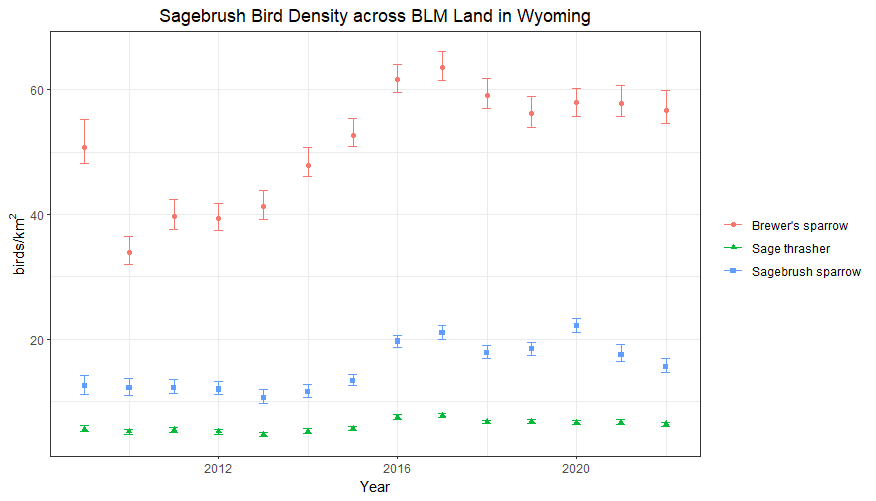
\includegraphics{./BLM-WY-density-trend.png}

}

\caption{\label{fig-blm-wy-sage}Density of three sagebrush-associated
species across all BLM land in Wyoming from 2009-2022, illustrating
stable to increasing population change.}

\end{figure}

Within several specific BLM field offices, however, populations for
these three species are decreasing and may require specific management
or conservation efforts to restore sagebrush rangelands. For example,
the Brewer's sparrow population is decreasing approximately 6\% each
year in the Lander Field Office, the sagebrush sparrow sparrow
population is decreasing 19\% per year in the Lander Field Office, and
the sage thrasher population in the Worland Field Office is decreasing
5\% each year (Table~{3}).

\begin{figure*}

\hypertarget{sec-table-3}{%
\paragraph{\texorpdfstring{\emph{Table 3. Population trend estimates for
sensitive sagebrush bird species within select Wyoming Bureau of Land
Management strata from the IMBCR
program.}}{Table 3. Population trend estimates for sensitive sagebrush bird species within select Wyoming Bureau of Land Management strata from the IMBCR program.}}\label{sec-table-3}}

\end{figure*}

\hypertarget{bird-conservation-region-17-1}{%
\subsection{Bird Conservation Region
17}\label{bird-conservation-region-17-1}}

We have also monitored across the Badlands and Prairies Bird
Conservation Region (BCR 17) since 2009. Grassland birds are among the
fastest declining group of birds in North America (Rosenberg et
al.~2019, NABCI 2022). Grassland prairie converted for cropland or
residential development threatens these populations on both the breeding
and wintering grounds (NABCI 2016), and the loss may be as high as 700
million breeding individuals over the past 50 years (Rosenberg et
al.~2019).

For the Northern Great Plains Joint Venture, the chestnut-collared
longspur and Sprague's pipit are focal species of conservation concern,
and are declining across this region (17\% each year for
chestnut-collared longspur and 26\% each year for Sprague's pipit;
Table~{4}). However, if we look at specific management units in BCR17,
local populations for these species are actually increasing:
chestnut-collared longspur by 4\% each year on Cedar River National
Grassland in North Dakota and Sprague's pipit by 17\% each year on Grand
River National Grassland in South Dakota (Table~{4}).

\begin{figure*}

\hypertarget{table-4.-population-trend-estimates-for-two-grassland-bird-species-within-bird-conservation-region-17-from-the-imbcr-program.-sec-table-4}{%
\paragraph{\texorpdfstring{\emph{Table 4. Population trend estimates for
two grassland bird species within Bird Conservation Region 17 from the
IMBCR program.
\{\#sec-table-4\}}}{Table 4. Population trend estimates for two grassland bird species within Bird Conservation Region 17 from the IMBCR program. \{\#sec-table-4\}}}\label{table-4.-population-trend-estimates-for-two-grassland-bird-species-within-bird-conservation-region-17-from-the-imbcr-program.-sec-table-4}}

\end{figure*}

Grassland birds often show low site fidelity from year-to-year as they
track suitable breeding sites (Cody 1985), emphasizing the need for
regional monitoring to identify these important breeding locations and
to track population change over time. In addition, the monitoring data
serve as a logical place to form hypotheses for observed population
fluctuations and predictions about bird response to drivers of change
(Pavlacky et al.~2017). For example, we could model abiotic and biotic
habitat features relevant for grassland birds to understand population
discrepancies between regional and local scales.

\hypertarget{usfs-rocky-mountain-region}{%
\subsection{USFS Rocky Mountain
Region}\label{usfs-rocky-mountain-region}}

The USFS Rocky Mountain Region has been involved in IMBCR since the
beginning in 2008, so we now have 15 years of monitoring data across
this region. Cassin's sparrow and olive-sided flycatcher are designated
sensitive species for the Rocky Mountain Region because of concern about
the population viability of these species on USFS land within the region
(USFS Manual 2670.5).

Cassin's sparrows are actually increasing across national grasslands in
this region (5\% each year; Figure~\ref{fig-usfs-grassland}), and
olive-sided flycatchers are also increasing about 4\% each year across
national forests in the region (Table~{5}). It's important to look at
trends within specific units, however, because populations may show
variable trends locally and could warrant a designation as Species of
Conservation Concern (36 CFR § 219.19).

\begin{figure*}

\hypertarget{table-5.-population-trend-estimates-for-sensitive-species-within-select-u.s.-forest-service-national-grassland-and-national-forest-strata-from-the-imbcr-program.-sec-table-5}{%
\paragraph{\texorpdfstring{\emph{Table 5. Population trend estimates for
sensitive species within select U.S. Forest Service National Grassland
and National Forest strata from the IMBCR program.
\{\#sec-table-5\}}}{Table 5. Population trend estimates for sensitive species within select U.S. Forest Service National Grassland and National Forest strata from the IMBCR program. \{\#sec-table-5\}}}\label{table-5.-population-trend-estimates-for-sensitive-species-within-select-u.s.-forest-service-national-grassland-and-national-forest-strata-from-the-imbcr-program.-sec-table-5}}

\end{figure*}

For instance, olive-sided flycatchers are decreasing 19\% each year on
the Arapaho and Roosevelt National Forests, but increasing 35\% per year
on the Shoshone National Forest (Table~{5}). Populations of western
forest species may be stable overall, but forests with a greater
departure from historical conditions shaped by frequent fire activity
could be hotspots for avian population declines (NABCI 2022).

Cassin's sparrows are decreasing 11\% each year on Cimarron National
Grassland, but increasing 3\% each year on Comanche National Grassland
(Table~{5}; Figure~\ref{fig-usfs-grassland}). Although many grassland
birds breed on privately owned land, publicly managed grasslands also
provide critical breeding habitat.

\begin{figure}

{\centering 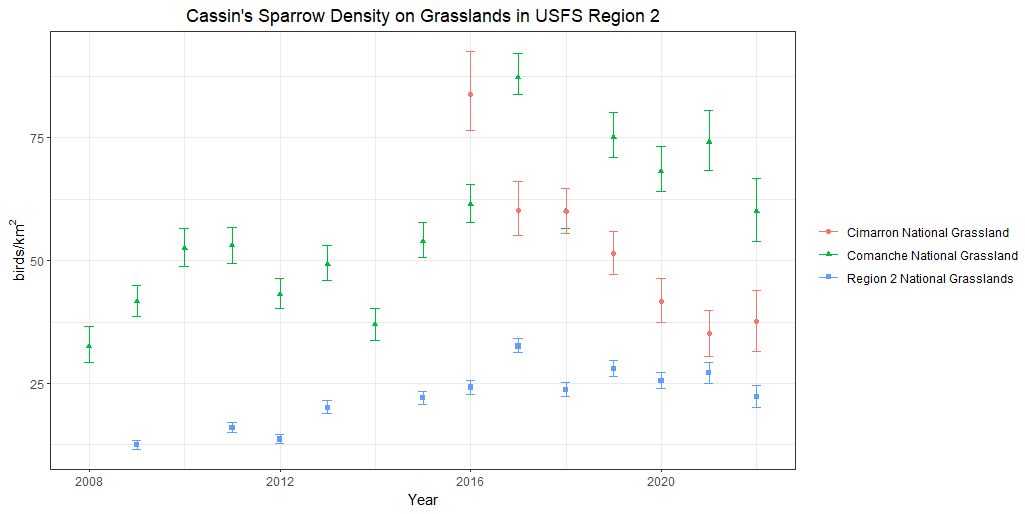
\includegraphics{./USFS-grassland-density-trend.png}

}

\caption{\label{fig-usfs-grassland}Density of Cassin's sparrows on
Comanche National Grassland, Cimarron National Grassland, and all
national grasslands in USFS Region 2 from 2008-2022 (2016-2022 for
Cimarron only), illustrating variable population trends at local and
regional scales.}

\end{figure}

\hypertarget{conclusions}{%
\chapter{Conclusions}\label{conclusions}}

The availability of consistent monitoring data at multiple scales is an
important challenge for avian conservation (Ruth et al., 2003). The
IMBCR program meets this challenge through its probabilistic, nested
design, which allows for inference to multiple scales of interest, from
National Grasslands to states to BCRs (Pavlacky et al., 2017). With this
design, we can model habitat relationships to evaluate species'
responses to local management actions and predict species' distributions
for landscape prioritization. Stratification based on eco-regional
boundaries and other fixed attributes is also a critical feature of the
IMBCR program because it allows for the evaluation of long-term avian
responses to landscape and climate change (Metzger et al., 2013;
Pavlacky et al., 2017).

The importance of long-term population monitoring at larger spatial
scales is well known (Jones, 2011; Thompson et al., 1998), but it is
often cost-prohibitive. The IMBCR program reduces expenses through
cooperation with multiple partners, one of the stated goals of effective
collaboration and coordinated bird monitoring (NABCI Monitoring
Subcommittee, 2007), and also through efficiencies in data collection
and analyses. Partners can investigate priority species and management
questions with slight modifications to the IMBCR design, further
reducing costs associated with developing new studies and monitoring
programs. These cost savings allow for an increased sampling effort
and/or for the development of decision support tools to aid land
managers and conservation practitioners on the ground. Based on the
spatially balanced design, the IMBCR program can also accommodate a
shortage of monitoring funds in certain years or strata without reducing
the overall rigor of the program (Stevens Jr.~\& Olsen, 2004).

The IMBCR program is well-positioned to address the conservation and
management needs of a wide range of stakeholders due to its rigorous,
hierarchical design and the strength of the IMBCR partnership. This
partnership is an ongoing collaboration between multiple entities from
state and federal agencies to non-governmental organizations and Joint
Ventures, and was created to address management and conservation
objectives of larger avian programs like NABCI (NABCI Monitoring
Subcommittee, 2007). Through the IMBCR partnership, monitoring resources
are pooled, creating efficiencies and allowing for inference to larger
landscapes (Pavlacky et al., 2017). By providing essential knowledge of
bird populations at multiple scales relevant to management and
conservation, the IMBCR program informs prioritization of management
actions and facilitates a collaborative approach to bird conservation
(Ruth et al., 2003, Pavlacky et al., 2017).

\bookmarksetup{startatroot}

\hypertarget{references}{%
\chapter*{References}\label{references}}
\addcontentsline{toc}{chapter}{References}

\markboth{References}{References}

\hypertarget{refs}{}
\begin{CSLReferences}{0}{0}
\end{CSLReferences}

Alexander, J. D., Stephens, J. L., Geupel, G. R., \& Will, T. C. (2008).
Decision support tools: bridging the gap between science and management.
In Proceedings of the Fourth International Partners in Flight
Conference: Tundra to Tropics. (p.~Pages 283--291). McAllen, Texas, USA.
Retrieved from
http://www.partnersinflight.org/pubs/McAllenProc/articles/PIF09\_Decision
Support Tools/Alexander\_PIF09.pdf

Arizona Game and Fish Department. (2012). Arizona's State Wildlife
Action Plan: 2012 - 2022. Arizona Game and Fish Department, Phoenix,
Arizona. Retrieved from
http://www.azgfd.gov/pdfs/w\_c/cwcs/downloads/CWCS\_Final\_May2006.pdf

Baron, J. S., Julius, S. H., West, J. M., Joyce, L. A., Blate, G.,
Peterson, C. H., \ldots{} Griffith, B. (2008). Some guidelines for
helping natural resources adapt to climate change. International Human
Dimensions Programme on Global Environmental Change Update, 2, 46--52.

Blakesley, J. A., \& Hanni, D. J. (2009). Monitoring Colorado's Birds,
2008 (No.~Tech. Rep.~M-MCB08-01.). Technical Report M-MCB08-01. Rocky
Mountain Bird Observatory, Brighton, Colorado, USA.

Brooks, T., Da Fonseca, G. A. and Rodrigues, A. S. (2004). Species,
Data, and Conservation Planning. Conservation Biology, 18, 1682-1688.

Buckland, S. T., Anderson, D. R., Burnham, K. P., Laake, J. L.,
Borchers, D. L., \& Thomas, L. (2001). Introduction to distance
sampling: estimating abundance of biological populations. Oxford, UK:
Oxford University Press.

Buckland, S. T., Marsden, S. J., \& Green, R. E. (2008). Estimating bird
abundance: making methods work. Bird Conservation International, 18,
S91--S108.

Bureau of Land Management. (2010). Wyoming Sensitive Species Policy and
List. Retrieved from
http://www.blm.gov/pgdata/etc/medialib/blm/wy/resources/efoia/IMs/2010.Par.41285.File.dat/wy2010-027atch2.pdf

Bureau of Land Management. (2014). 2014 Montana/Dakotas BLM Special
Status Species List.

Bureau of Land Management. (2015). Idaho Bureau of Land Management
Special Status Species List Update. Idaho State Office Instruction
Memorandum 2015-009c1, attachment 1. Chesser, R. T., Burns, K. J.,
Cicero, C., Dunn, J. L., Kratter, A. W., Lovette, I. J., \ldots{}
Winker, K. (2017). Fifty-eighth supplement to the American
Ornithological Society's Check-list of North American Birds. The Auk,
134(3), 751--773.

Chesser, R. T., S. M. Billerman, K. J. Burns, C. Cicero, J. L. Dunn, B.
E. Hernández-Baños, R. A. Jiménez, A. W. Kratter, N. A. Mason, P. C.
Rasmussen, J. V. Remsen, Jr., D. F. Stotz, and K. Winker. 2022.
Check-list of North American Birds (online). American Ornithological
Society. \url{https://checklist.americanornithology.org/taxa/}

Cody, M. L. (1985). Habitat selection in birds. New York, NY, USA.
Academic Press.

Colorado Parks and Wildlife. (2015). Vertebrate and Mollusk Species of
Greatest Conservation Need. Retrieved from
http://cpw.state.co.us/Documents/WildlifeSpecies/SWAP/SGCN-Final-Table.pdf

Correll, M. D., Drilling, N., Dwyer, A., George, T. L., Green, A. W.,
Panjabi, A. O., Pavlacky Jr., D. C., Quattrini, L., Shaw, A., Sparks, R.
A., Strasser, E. H., \& Van Boer, A. (2016). Recommendations for
grassland bird species conservation in the Northern Great Plains
business plan. Final report. Bird Conservancy of the Rockies, Brighton,
Colorado, USA.

Dreitz, V. J., Lukacs, P. M., \& Knopf, F. L. (2006). Monitoring low
density avian populations: An example using Mountain Plovers. Condor,
108(3), 700--706.

Dreitz, V. J., Stinson, L. T., Hahn, B. A., Tack, J. D., \& Lukacs, P.
M. (2017). A large-scale perspective for managing prairie avifauna
assemblages across the western US: influences of habitat, land ownership
and latitude. PeerJ, 5, e2879. https://doi.org/10.7717/peerj.2879

Dyke, S. R., Johnson, S. K., Isakson, P. T. (2015). North Dakota State
Wildlife Action Plan. North Dakota Game and Fish Department, Bismarck,
ND. 438 pp. Environmental Systems Research Institute. (2017). ArcGIS,
version 10.X. Redlands, California, USA: Environmental Systems Research
Institute, Incorporated.

Green, A. W., Pavlacky, D. C., \& George, T. L. (2019). A dynamic
multi-scale occupancy model to estimate temporal dynamics and
hierarchical habitat use for nomadic species. Ecology and Evolution,
2019(9), 793-803.

Hanni, D. J., White, C. M., Birek, J. J., Van Lanen, N. J., \& McLaren,
M. F. (2012). Field protocol for spatially-balanced sampling of landbird
populations. Unpublished report. Brighton, Colorado, USA: Rocky Mountain
Bird Observatory. Retrieved from
http://rmbo.org/v3/Portals/5/Protocols/2012\%20Field\_protocol\_for\_spacially\_balanced\_sampling\_final.pdf

Hewitt JE, Thrush SF, Dayton PK, Bonsdorff E. 2007. The effect of
spatial and temporal heterogeneity on the design and analysis of
empirical studies of scale-dependent systems. American Naturalist
169:398--408.

Hobbs, N. T., \& Hooten, M. B. (2015). Bayesian models: a statistical
primer for ecologists. Princeton University Press, Princeton, New
Jersey, USA.

Johnson, D. H. (1980). The Comparison of Usage and Availability
Measurements for Evaluating Resource Preference. Ecology, 61(1), 65--71.
https://doi.org/10.2307/1937156

Jones, J. P. G. (2011). Monitoring species abundance and distribution at
the landscape scale. Journal of Applied Ecology, 48(1), 9--13.
https://doi.org/10.1111/j.1365-2664.2010.01917.x

Kellner, K. (2018). Package `jagsUI'.
https://cran.r-project.org/web/packages/jagsUI/jagsUI.pdf. Accessed 2
Jul 2019.

Knick, S.T., and Rotenberry, J.T., 2002. Effects of habitat
fragmentation on passerine birds 587 breeding in Intermountain
shrubsteppe. Studies in Avian Biology 25:131--141.

Lindenmayer, D. B., \& Likens, G. E. (2009). Adaptive monitoring: a new
paradigm for long-term research and monitoring. Trends in Ecology and
Evolution, 24(9), 482--486.

Lindenmayer, D. B., \& Likens, G. E. (2010). The science and application
of ecological monitoring. Biological Conservation, 143(6), 1317--1328.
https://doi.org/10.1016/j.biocon.2010.02.013

Lyons, J. E., Runge, M. C., Laskowski, H. P., \& Kendall, W. L. (2008).
Monitoring in the context of structured decision-making and adaptive
management. The Journal of Wildlife Management, 72 (8), 1683--1692.

MacKenzie, D. I., Nichols, J. D., Lachman, G. B., Droege, S., Royle, J.
A., \& Langtimm, C. A. (2002). Estimating site occupancy rates when
detection probabilities are less than one. Ecology, 83(8), 2248--2255.

MacKenzie, D. I., Nichols, J. D., Royle, J. A., Pollock, K. H., Bailey,
L. L., \& Hines, J. E. (2006). Occupancy estimation and modeling:
inferring patterns and dynamics of species occurrence. Burlington,
Massachusetts, USA: Elsevier.

Manley, P. N., Schlesinger, M. D., Roth, J. K., \& Van Horne, B. (2005).
A field-based evaluation of a presence-absence protocol for monitoring
ecoregional-scale biodiversity. Journal of Wildlife Management, 69(3),
950--966.

Marsh, D. M., \& Trenham, P. C. (2008). Current trends in plant and
animal population monitoring. Conservation Biology, 22(3), 647--655.

Metzger, M. J., Brus, D. J., Bunce, R. G. H., Carey, P. D., Gonçalves,
J., Honrado, J. P., \ldots{} Zomer, R. (2013). Environmental
stratifications as the basis for national, European and global
ecological monitoring. Ecological Indicators, 33, 26--35.
https://doi.org/10.1016/j.ecolind.2012.11.009

Montana Fish Wildlife and Parks. (2015). Montana State Wildlife Action
Plan, 1--453. https://doi.org/10.1017/CBO9781107415324.004

Montana Natural Heritage Program. (2015). Animal Species of Concern.
Retrieved April 1, 2015, from http://mtnhp.org/SpeciesOfConcern/

Mordecai, R. S., Mattsson, B. J., Tzilkowski, C. J., \& Cooper, R. J.
(2011). Addressing challenges when studying mobile or episodic species:
Hierarchical Bayes estimation of occupancy and use. Journal of Applied
Ecology 48: 56--66. https://doi.org/10.1111/j.1365-2664.2010.01921.

New Mexico Department of Game and Fish. (2016). State Wildlife Action
Plan for New Mexico. New Mexico Department of Game and Fish. Santa Fe,
New Mexico. Retrieved from
http://www.wildlife.state.nm.us/download/conservation/swap/New-Mexico-State-Wildlife-Action-Plan-SWAP-Final-2017.pdf

Nichols, J. D., Bailey, L. L., O'Connell, A. F., Talancy, N. W., Grant,
E. H. C., Gilbert, A. T., \ldots{} Hines, J. E. (2008). Multi-scale
occupancy estimation and modelling using multiple detection methods.
Journal of Applied Ecology, 45(5), 1321--1329.

Nichols, J. D., \& Williams, B. K. (2006). Monitoring for conservation.
Trends in Ecology and Evolution, 21(12), 668--673.

Noon, B. R., Bailey, L. L., Sisk, T. D., \& McKelvey, K. S. (2012).
Efficient Species-Level Monitoring at the Landscape Scale. Conservation
Biology, 26(3), 432--441.

North American Bird Conservation Initiative. (2016). The State of North
America's Birds 2016. Environment and Climate Change Canada: Ottawa,
Ontario. 8 pages. www.stateofthebirds.org

North American Bird Conservation Initiative. 2022. The State of the
Birds, United States of America, 2022. StateoftheBirds.org

Oklahoma Department of Wildlife Conservation. (2015). Oklahoma
Comprehensive Wildlife Conservation Strategy: A Strategic Conservation
Plan for Oklahoma's Rare and Declining Wildlife Retrieved from
https://www.wildlifedepartment.com/wildlifemgmt/cwcs.pdf

Opdam, P., \& Wascher, D. (2004). Climate change meets habitat
fragmentation: linking landscape and biogeographical scale levels in
research and conservation. Biological Conservation, 117(3), 285--297.

Partners in Flight. (2017). Avian Conservation Assessment Database,
version 2017. Retrieved March 7, 2018, from
http://pif.birdconservancy.org/ACAD

Pavlacky, D. C., Lukacs, P. M., Blakesley, J. A., Skorkowsky, R. C.,
Klute, D. S., Hahn, B. A., \ldots{} Hanni, D. J. (2017). A statistically
rigorous sampling design to integrate avian monitoring and management
within Bird Conservation Regions. PLoS ONE, 12(10).
https://doi.org/10.1371/journal.pone.0185924

Pavlacky Jr., D. C., Blakesley, J. A., White, G. C., Hanni, D. J., \&
Lukacs, P. M. (2012). Hierarchical multi-scale occupancy estimation for
monitoring wildlife populations. Journal of Wildlife Management, 76,
154--162.

Plummer, M. (2003). JAGS: a program for analysis of Bayesian graphical
models using Gibbs sampling. Proceedings of the 3rd International
Workshop on Distributed Statistical Computing DSC 2003, 20--22 March
2003, Vienna, Austria.

Plummer, M. (2017). JAGS version 4.3.0 user manual.
https://sourceforge.net/projects/mcmc-jags/files/Manuals/4.x/jags\_user\_manual.pdf/download.
Accessed 2 Jul 2019.

Pollock, K. H. (1982). A capture-recapture design robust to unequal
probability of capture. Journal of Wildlife Management, 46(3), 752--757.

Pollock, K. H., Nichols, J. D., Simons, T. R., Farnsworth, G. L.,
Bailey, L. L., \& Sauer, J. R. (2002). Large scale wildlife monitoring
studies: statistical methods for design and analysis. Environmetrics,
13(2), 105--119. https://doi.org/10.1002/env.514

R Core Team. (2019). R: a language and environment for statistical
computing. Vienna, Austria: R Foundation for Statistical Computing.
Retrieved from www.R-project.org/

Rich, T. D., Beardmore, C. J., Berlanga, H., Blancher, P. J.,
Bradstreet, M. S. W., Butcher, G. S., \ldots{} Will, T. C. (2004).
Partners in Flight North American landbird conservation plan. Ithaca,
New York, USA: Cornell Lab of Ornithology.

Rosenstock, S. S., Anderson, D. R., Giesen, K. M., Leukering, T., \&
Carter, M. F. (2002). Landbird counting techniques: current practices
and an alternative. Auk, 119(1), 46--53.

Royle, J. A., Dawson, D. K., \& Bates, S. (2004). Modeling abundance
effects in distance sampling. Ecology, 85(6), 1591-1597.

Ruggiero, L. F., Hayward, G. D., \& Squires, J. R. (1994). Viability
analysis in biological evaluations: Concepts of population vability
analysis, biological population, and ecological scale. Conservation
Biology, 8(2), 364--372.

Ruth, J. M., Petit, D. R., Sauer, J. R., Samuel, M. D., Johnson, F. A.,
Fornwall, M. D., Bennett, J. P. (2003). Science for avian conservation:
Priorities for the new millennium. Auk, 120(1), 204--211.

Sauer, J. R., \& Knutson, M. G. (2008). Objectives and metrics for
wildlife monitoring. Journal of Wildlife Management, 72(8), 1663--1664.

Schneider, R., Fritz, M., Jorgensen, J., Schainost, S., Simpson, R.,
Steinauer, G., \& Rothe-Groleau, C.. (2018). Revision of the Tier 1 and
2 Lists of Species of Greatest Conservation Need: A Supplement to the
Nebraska Natural Legacy Project State Wildlife Action Plan. The Nebraska
Game and Parks Commission, Lincoln, NE.

Sillett, T. S., Chandler, R. B., Royle, J. A., Kéry, M., \& Morrison,
S.A. (2012). HIerarchical distance-sampling models to estimate
population size and habitat-specific abundance of an island endemic.
Ecological Applications, 22(7), 1997-2006.

Sparks, R. A., \& Hanni, D. J. (2013). Monitoring Birds on Little
Missouri, Sheyenne and Grand River National Grasslands. Tech. Report \#
M-DAKPG-12. Rocky Mountain Bird Observatory, Brighton, Colorado, USA.

Sparks R. A., Van Lanen, N. J., Van Boer, A. \& Pavlacky Jr., D. C.
(2016). Monitoring Avian Populations on Colorado and Wyoming Military
Installations. Bird Conservancy of the Rockies. Brighton, Colorado, USA.

Stevens Jr., D. L., \& Olsen, A. R. (2004). Spatially balanced sampling
of natural resources. Journal of the American Statistical Association,
99(465), 262--278.

Texas Parks and Wildlife Department. (2012). Texas Conservation Action
Plan 2012 - 2016. Austin, TX.

Thomas, L., Buckland, S. T., Rexstad, E. A., Laake, J. L., Strindberg,
S., Hedley, S. L., \ldots{} Burnham, K. P. (2010). Distance software:
design and analysis of distance sampling surveys for estimating
population size. Journal of Applied Ecology, 47, 5--14.

Thompson, W. L. (2002). Towards reliable bird surveys: accounting for
individuals present but not detected. Auk, 119(1), 18--25.

Thompson, W. L., White, G. C., \& Gowan, C. (1998). Monitoring
vertebrate populations. San Diego, California, USA: Academic Press.

US Forest Service. (2008). Region 2 Regional Forester's Sensitive
Species. Retrieved from
http://www.fs.fed.us/r2/projects/scp/sensitivespecies/index.shtml.

US North American Bird Conservation Initiative. (2000). Bird
Conservation Regions descriptions: a supplement to the North American
Bird Conservation Initiative: Bird Conservation Regions map.

US North American Bird Conservation Initiative. (2009). The State of the
Birds, United States of America, 2009. Washington, D.C., USA: U.S.
Department of Interior. Retrieved from
http://www.stateofthebirds.org/pdf\_files/State of the Birds\_FINAL.pdf

US North American Bird Conservation Initiative Monitoring Subcommittee.
(2007). Opportunities for improving avian monitoring. Arlington,
Virginia, USA: Division of Migratory Bird Management, U.S. Fish and
Wildlife Service. Retrieved from
http://www.nabci-us.org/aboutnabci/monitoringreportfinal0307.pdf

Utah Wildlife Action Plan Joint Team. (2015). Utah Wildlife Action Plan:
A plan for managing native wildlife species and their habitats to help
prevent listing under the Endangered Species Act. Salt Lake City, Utah,
USA: Utah Division of Wildlife Resources.

Watanabe, S. (2010). Asymptotic equivalence of Bayes cross validation
and widely applicable information criterion in singular learning theory.
Journal of Machine Learning Research, 2010(11), 3571-3594.

Wiens, J. A., Rotenberry, J. T., \& Van Horne, B. (1987). Habitat
Occupancy Patterns of North American Shrubsteppe Birds: The Effects of
Spatial Scale. Oikos, 48(2), 132. https://doi.org/10.2307/3565849

Wilson, K. A., Underwood, E. C., Morrison, S. A., Klausmeyer, K. R.,
Murdoch, W. W., Reyers, B., \ldots{} Possingham, H. P. (2007).
Conserving biodiversity efficiently: What to do, where, and when. PLoS
Biology, 5(9), 1850--1861. https://doi.org/10.1371/journal.pbio.0050223

Witmer, G. W. (2005). Wildlife population monitoring: some practical
considerations. Wildlife Research, 32, 259--263.

Wyoming Game and Fish Department. (2016). 2017 Species of Greatest
Conservation Need. Retrieved from
https://wgfd.wyo.gov/WGFD/media/content/PDF/Habitat/SWAP/Wyoming-SGCN.pdf

\appendix
\addcontentsline{toc}{part}{Appendices}

\hypertarget{rocky-mountain-avian-data-center-tips}{%
\chapter{Rocky Mountain Avian Data Center
Tips}\label{rocky-mountain-avian-data-center-tips}}

All results, including parameter estimates, distribution maps, raw count
data and effort, are available online. To view interactive maps showing
survey and detection locations, as well as species counts, and density,
population and occupancy results using the IMBCR study design please
visit the Rocky Mountain Avian Data Center. Click on the ``Explore the
Data'' tab to view IMBCR results.

\hypertarget{selecting-filters}{%
\subsection*{Selecting filters}\label{selecting-filters}}
\addcontentsline{toc}{subsection}{Selecting filters}

The Rocky Mountain Avian Data Center has been designed to provide
information for specific questions and therefore works best when users
select multiple filters for a query.

To run a query, click the arrow for the drop down ``Filter'' menu
(located in the extreme upper left corner of the screen) and select one
of the following filter types: Study Design, BCR, State, County,
Management Entity, Priority Species List, Species, Year, Superstratum,
or Individual Stratum. After selecting the filter type, click the
``Add'' button immediately to the right of the drop down menu. A box
will appear with options for the filter that you may select. Use the
drop down menu in the box to select the specific filter and then click
``Add filter''.

The selected filter will appear near the top of the screen. Users may
add multiple filter types to view results for a very specific inquiry
(e.g., to view IMBCR results for BRSP in CO you would apply the
following filters: Study Design = IMBCR, Species = Brewer's Sparrow and
State = CO) or to view multiple outputs at once (e.g., to view data and
results for Brewer's Sparrow and Vesper Sparrow at the same time select
Species = Brewer's Sparrow and Species = Vesper Sparrow). Below is an
explanation of the different filter types you may choose from.

\textbf{Study Design}: This filter will allow users to select data and
results for IMBCR, GRTS, Migration Phenology, NEON, or NPS study
designs.

\begin{quote}
\begin{itemize}
\item
  Selecting the GRTS filter will display data and results for monitoring
  efforts which used the IMBCR design but do NOT contribute to statewide
  and regional estimates (also known as ``overlays'').
\item
  The IMBCR filter will select data and results collected under the
  IMBCR protocol that contribute to state and BCR-wide estimates.
\item
  The Migration Phenology filter will select data and results for the
  Migration Phenology project.
\item
  The NEON study design is a specific study design developed by NEON and
  Bird Conservancy for surveys conducted at NEON research locations.
\item
  The NPS study designs are a mixture of study designs specifically
  designed for individual national parks. Please note that we are still
  working on adding some of the historic data to the Avian Data Center
  so not all study designs are currently available.
\end{itemize}
\end{quote}

\textbf{BCR}: This filter will allow users to select data and results
for a particular Bird Conservation Region. Selecting this filter will
provide you with results for all strata and superstrata within a
particular BCR.

\textbf{State}: This filter will allow users to select data and results
for all study designs for a particular state. Selecting this filter will
supply the user with data and results for all strata and superstrata
within a particular state.

\textbf{County}: This filter will allow users to select data for a
particular county. Please note that only raw count data and survey
locations are available at the county level.

\textbf{Priority Species List}: This filter will allow users to select
data and results for multiple species at once. The query will display
data and results for all species included on the selected management
indicator list, species of conservation concern list, etc.

\textbf{Species}: This filter allows users to select data and results
for a particular species.

\textbf{Year}: This filter will allow users to select all data and
results for a particular year.

\textbf{Superstratum}: This filter allows users to select IMBCR data and
results for multiple strata that were analyzed jointly (e.g., the entire
Bridger-Teton National Forest which was broken up into 2 strata or the
entire state of Colorado which was broken up into 30 strata).

\textbf{Management Entity}: This filter will allow users to select data
and results for All Other Lands, Colorado State Land Board, The Nature
Conservancy (TNC), US Bureau of Indian Affairs (BIA), US Bureau of Land
Management (BLM), US Department of Defense (DOD), US Fish and Wildlife
Service (USFWS), US Forest Service (USFS), or National Park Service
(NPS). Once a management entity is chosen, users may notice that
additional filter types are available in the filters drop down list.
These additional filter types, listed from most general to most
specific, are management regions (e.g., USFS Region 1), management units
(e.g., Dakota Prairie Grasslands), management forests (e.g., Shoshone
National Forest), or management districts (e.g., North Kaibab district
within Kaibab National Forest). Below is the filter hierarchy for the
different management entities.

\textbf{Hierarchy for the different management entities}

\begin{quote}
\textbf{All Other Lands:}

Tier One -- Management Entity -- All Other Lands\\
Tier Two -- Management Region -- n/a\\
Tier Three -- Management Unit -- n/a\\
Tier Four -- National Forest or Grassland -- n/a\\
Tier Five -- Management District -- n/a

\textbf{Colorado State Land Board:}

Tier One -- Management Entity -- Colorado State Land Board\\
Tier Two -- Management Region -- Lowry Range\\
Tier Three -- Management Unit -- n/a\\
Tier Four -- National Forest or Grassland -- n/a\\
Tier Five -- Management District -- n/a

\textbf{TNC:}

Tier One -- Management Entity -- The Nature Conservancy\\
Tier Two -- Management Region -- Cherry Creek\\
Tier Three -- Management Unit -- n/a\\
Tier Four -- National Forest or Grassland -- n/a\\
Tier Five -- Management District -- n/a

\textbf{Tribal Lands:}

Tier One -- Management Entity -- US Bureau of Indian Affairs\\
Tier Two -- Management Region -- Reservation\\
Tier Three -- Management Unit -- n/a\\
Tier Four -- National Forest or Grassland -- n/a\\
Tier Five -- Management District -- n/a

\textbf{BLM:}

Tier One -- Management Entity -- Bureau of Land Management\\
Tier Two -- Management Region -- BLM Field Office\\
Tier Three -- Management Unit -- n/a\\
Tier Four -- National Forest or Grassland -- n/a\\
Tier Five -- Management District -- n/a

\textbf{DOD:}

Tier One -- Management Entity -- US Department of Defense\\
Tier Two -- Management Region -- US DoD Installation\\
Tier Three -- Management Unit -- n/a\\
Tier Four -- National Forest or Grassland -- n/a\\
Tier Five -- Management District -- n/a

\textbf{USFWS:}

Tier One -- Management Entity -- US Fish and Wildlife Service\\
Tier Two -- Management Region -- USFWS Region Tier Three -- Management
Unit -- USFWS Management Unit, Refuge, etc.\\
Tier Four -- National Forest or Grassland -- n/a Tier Five -- Management
District -- n/a

\textbf{USFS:}

Tier One -- Management Entity -- US Forest Service\\
Tier Two -- Management Region -- USFS Regions\\
Tier Three -- Management Unit -- National Forest (NF) or National
Grassland (NG) management units (used to represent situations where
multiple forests are managed jointly)\\
Tier Four -- National Forest or Grassland -- NF or NG\\
Tier Five -- Management District -- NF or NG Ranger Districts

\textbf{NPS:}

Tier One -- Management Entity -- National Park Service\\
Tier Two -- Management Region -- Inventory and Monitoring Network\\
Tier Three -- Management Unit -- Individual NPS Parks, Monuments,
Memorials, Recreation Areas, and Historic Sites\\
Tier Four -- Management Forest -- n/a\\
Tier Five -- Management District -- n/a
\end{quote}

\textbf{\emph{Clearing Filters}}

Filters can be cleared in one of two ways. You may click on the circled
``X'' to the left of an individual filter at the top of the screen to
remove it or you may click the ``clear all filters'' button at the top
of the screen to start building a new query.

\textbf{\emph{Running Queries}}

Once you have selected your desired filters, please click on the ``Run
Query'' button located at the top of the screen. The amount of time it
takes for the desired data and results to be displayed will depend on
how specific your query is.

\textbf{\emph{Comparing Multiple Queries}}

Users may view results of multiple queries at once. To do this, run the
first query as described above and then click the button ``New Query
Window'' (located at the top of the screen). A new window will appear
where a separate query can be run. The two windows can then be viewed
side by side.

\textbf{\emph{Share a Created Query with a Colleague}}

It is possible to create a link to the Avian Data Center/ Explore the
Data screen with a pre-loaded set of filters for a query. To do this,
add the custom set of filters for your query per the instructions above
and then click the ``Generate URL'' button near the top right corner of
the screen. A pop-up box will appear with a highlighted URL address.
Once you copy the highlighted text, you may paste the URL address into
an email or document using conventional means. Please note that whoever
receives the URL address will need to run the query after clicking on
the link to see the survey locations, results, and raw count statistics
for the set of filters of interest.

\hypertarget{viewing-maps-map-tab}{%
\section*{Viewing Maps (Map Tab)}\label{viewing-maps-map-tab}}
\addcontentsline{toc}{section}{Viewing Maps (Map Tab)}

\markright{Viewing Maps (Map Tab)}

\textbf{\emph{What is displayed}}

By default, the map tab is the initial start-up page. After clicking the
``Run Query'' button, the ADC will display a map of all survey locations
corresponding to your set of filters (surveyed sampling units are
represented by blue semi-transparent circles) using Google Maps. If you
have filtered by species, blue circles represent survey locations where
that species was not detected and blue circles with a pink dot in the
center represent survey locations where that species was detected. To
see the specific name of a survey location, hover the mouse arrow over
the blue circle. After a moment the name of the surveyed sampling unit
will appear. You may view the bird detection information for a sampling
unit and the survey dates by left clicking your mouse on the blue
circle.

By default, the zoom capability of the maps page is restricted to
protect the privacy of private landowners. Funding and/or implementation
partners wishing for more precise location information to be displayed
should request a password from Bird Conservancy IT staff via email. Once
a user has a password, click on the ``View Options'' button at the top
of the screen, enter the password in the ``Password for Bird Conservancy
staff and partners'' field, and click ``Save''. If you have run a query
prior to entering the password, you will need to click the ``Run Query''
button again in order to utilize the enhanced zooming features now
available to you.

\textbf{\emph{Adding map layers}}

You may add the following layers to the map: Bird Conservation Region
boundaries, BIA boundaries, DoD boundaries, NPS boundaries, USFS
boundaries and BLM Field Office boundaries. To do this, left click on
the drop down menu at the top left corner of the map, select the desired
layer, and click the ``add layer'' button. It is possible to add
multiple layers to the map by repeating this process. The top-most
feature's name will appear if you left click your mouse inside the
layer's boundaries.

\hypertarget{viewing-occupancydensity-results-occupancy-and-density-tabs}{%
\section*{Viewing Occupancy/Density Results (Occupancy and Density
Tabs)}\label{viewing-occupancydensity-results-occupancy-and-density-tabs}}
\addcontentsline{toc}{section}{Viewing Occupancy/Density Results
(Occupancy and Density Tabs)}

\markright{Viewing Occupancy/Density Results (Occupancy and Density
Tabs)}

\textbf{\emph{Viewing Tables}}

You may view occupancy or density results table and a chart for all
appropriate strata (based on the set of filters) for which we have
results, by clicking on the tabs labeled ``Occupancy'' or ``Density''.
These tabs are located just below the drop down filter menu in the upper
left corner of the screen. The occupancy tables display species,
stratum, year, Psi (proportion of sampling units expected to be
occupied), number of sampling units the species was detected on,
standard error (SE) of the estimate, the percent coefficient of
variation (\% CV). The density tables will display species, stratum,
year, number of birds estimated per km² (D), total number of individuals
estimated within the stratum (N), percent coefficient of variation (\%
CV), and the number of independent detections used in analyses (n). You
may view a description of the column headings by moving the cursor over
the column heading.

\textbf{\emph{Viewing the Charts}}

When viewing the occupancy and density charts, the point estimate of Psi
or D is indicated with a dot. Additionally, short horizontal dashes
above and below the point estimate represent values one standard error
away from the point estimate. To view the species, stratum and year that
correspond to an estimate on the chart, simply move your mouse arrow
over the point estimate or standard error bar. A message will pop up
with the appropriate information. If you have queried out multiple years
of data, the point estimates for each year will be connected with a
solid line. You may remove an individual estimate from the chart by
clicking on the corresponding row of the table on the left side of the
screen. Estimates that are not displayed on the chart will turn a peach
color in the table. You may add the estimate back onto the chart by
clicking on the peach colored row in the table.

\textbf{\emph{Knowing which species have estimates}}

To restrict the species filter to display only those species for which
occupancy and/or density estimates have been produced, click on the
``View Options'' button on the very top of the screen and then check the
box next to ``Only show species for which occupancy/density results are
available''. This will prevent you from querying out numerous species
for which occupancy or density estimates are not available.

\textbf{\emph{Saving results of your query}}

You may easily save the results of your query by clicking the ``Copy to
clipboard'' button and pasting the results into another program such as
excel or by clicking the ``Save to CSV'' button. Similarly, to save a
chart click on the ``View Image'' button below the chart, right click on
anywhere on the image and select ``Copy image'' or ``Save image as''.

\textbf{\emph{Functionality}}

Please keep in mind that queries with very generic filters will result
in long wait times and may not function optimally (your browser may end
up crashing). For instance, if a user selects only the IMBCR filter,
occupancy results will be displayed for every species and
strata/superstrata combination for which there are occupancy and/or
density results. If your query is not specific enough, the chart on the
right side of the screen will not be displayed or a pop-up box will
appear asking if you would like to continue. This pop-up box is designed
to prevent your web browser from crashing while the RMADC attempts to
create a chart that would be extremely difficult to interpret. We
recommend that you cancel the proposed query and add additional filters
to make your query less generic.

\hypertarget{viewing-raw-count-statistics-species-counts-tab}{%
\section*{Viewing Raw Count Statistics (Species Counts
Tab)}\label{viewing-raw-count-statistics-species-counts-tab}}
\addcontentsline{toc}{section}{Viewing Raw Count Statistics (Species
Counts Tab)}

\markright{Viewing Raw Count Statistics (Species Counts Tab)}

You may view the raw count of detections for each species and the effort
(expressed as the number of point count stations surveyed) for your
query by clicking on the ``Species Counts'' tab located just below the
drop down filter menu in the upper left corner of the screen. Both the
counts (left table) and effort tables (right table) may be sorted by
clicking on the row header. Additionally, you may view the counts and
effort by BCR, State, County, Stratum, or Management Entity by clicking
on the ``Count by'' drop down menu located above the counts table. If
you have filtered using ``Superstrata'', viewing counts by Stratum is an
excellent way of getting a list of all the strata that comprise a
Superstratum. If you would prefer to view effort expressed as the number
of sampling units surveyed, click on the ``View Options'' button located
at the top of the screen and check the box labeled ``Show effort by
number of sampling units instead of by point''.

\hypertarget{imbcr-program-and-stratification-history}{%
\chapter{IMBCR Program and Stratification
History}\label{imbcr-program-and-stratification-history}}

In 1995, Bird Conservancy of the Rockies (Bird Conservancy; formerly
Rocky Mountain Bird Observatory), in partnership with Colorado Parks and
Wildlife (CPW; formerly Colorado Division of Wildlife), the United
States Forest Service (USFS), the Bureau of Land Management (BLM) and
the National Park Service (NPS), began efforts to create and conduct a
Colorado-wide program to monitor breeding bird populations. This was the
first attempt in the nation to develop and implement a statewide
landbird monitoring program. After a successful pilot year in 1998, Bird
Conservancy implemented the protocol in 13 habitats in Colorado in 1999.
Bird Conservancy and its partners used this methodology for 10 years and
expanded the effort to include parts of Arizona, New Mexico, North
Dakota, South Dakota, Utah, and Wyoming.

In 2007, the NABCI Monitoring Subcommittee published ``Opportunities for
Improving Avian Monitoring'' (NABCI Monitoring Subcommittee, 2007) which
offered recommendations for improving the efficiency and effectiveness
of avian monitoring in North America. After taking NABCI's
recommendations into consideration, IMBCR partners developed a new study
design and protocol for statewide bird monitoring in Colorado. The new
study design used BCRs as the sampling frame and further stratified by
land ownership within each BCR.

IMBCR partners stratified and surveyed the Southern Rockies/Colorado
Plateau BCR (BCR 16) and the Shortgrass Prairie BCR (BCR 18) portions of
Colorado, as well as the BCR 16 portion of Wyoming. Furthermore, in
Colorado BCR 16, we used cell weighting to target high order rivers and
streams (based on Strahler stream order) and higher elevation habitats
(e.g.~alpine tundra), which occur in a small proportion of the landscape
(Blakesley \& Hanni, 2009).

\hypertarget{section}{%
\section*{\texorpdfstring{\textbf{2009}}{2009}}\label{section}}
\addcontentsline{toc}{section}{\textbf{2009}}

\markright{\textbf{2009}}

After the 2008 season, IMBCR partners determined the cell weighting had
caused middle-elevations in Colorado to be under-sampled. To correct
this, all strata in the Colorado and Wyoming portions of BCR 16 were
re-stratified without cell weighting. Additionally, the All Other Lands
stratum in Wyoming BCR 16 was split into two strata: All Other Lands and
BLM Lands.

Based on the overall success of the pilot implementation, IMBCR expanded
to include the Colorado and Wyoming portions of the Northern Rockies
(BCR 10); the Great Basin (BCR 9) and BCR 18 portions of Wyoming; all of
the Badlands and Prairies (BCR 17); the USFS National Forests and
Grasslands within BCR 18; and Coconino and Prescott National Forests in
the Sierra Madre Occidental (BCR 34).

\hypertarget{section-1}{%
\section*{\texorpdfstring{\textbf{2010}}{2010}}\label{section-1}}
\addcontentsline{toc}{section}{\textbf{2010}}

\markright{\textbf{2010}}

The program expanded to include the BCR 10 and the Prairie Potholes BCR
(BCR 11) portions of Montana, three national forests in the Idaho
portion of BCR 10 and Kaibab National Forest in BCRs 16 and 34.
Additionally, there were several re-stratifications done in Colorado
BCRs 10 and 16 between 2009 and 2010. The Colorado BCR 10 stratum was
re-stratified to include the small easternmost portion of BCR 10 that
dips into Colorado so all Colorado BCR 10 lands are represented. The
``NPS Rocky Mountain Inventory and Monitoring Network (RMNW)'' and
``Northern Colorado Plateau Inventory and Monitoring Network (NCPN)''
were re-stratified because some NCPN park units were initially
misclassified into the RMNW stratum. In Wyoming, the USFS Region 4
stratum was re-stratified into three separate strata: ``Bridger-Teton
National Forest front-country/managed areas'', ``Bridger-Teton National
Forest designated roadless/wilderness areas'' and ``the remainder of
USFS Region 4 lands in Wyoming BCR 10''. This re-stratification was done
to allow for density and occupancy estimation specifically for the
Bridger-Teton National Forest.

\hypertarget{section-2}{%
\section*{\texorpdfstring{\textbf{2011}}{2011}}\label{section-2}}
\addcontentsline{toc}{section}{\textbf{2011}}

\markright{\textbf{2011}}

The geographic extent of the IMBCR program expanded to the Nebraska
portion of the Central Mixed Grass Prairie (BCR 19) and included all of
the national forests and grasslands in Nebraska. Additionally, there
were several re-stratifications done in Colorado. The Colorado BCR 10
stratum was split into two strata: BLM Lands and All Other Lands. This
was done to facilitate improved tracking of priority species on BLM
lands throughout Colorado. Rio Grande National Forest and White River
National Forest strata were each split into three strata: low, medium,
and high elevations. This stratification by elevation allowed sampling
intensity changes to target Management Indicator Species on the forests.
The Routt National Forest and Arapaho and Roosevelt National Forests
strata were reorganized and a third stratum, the Williams Fork Area, was
created from the two because it had mixed administration between the
Routt National Forest and the Arapahoe and Roosevelt National Forests.

The RMNW stratum was re-stratified to accurately reflect land ownership.
There was a land acquisition within Great Sand Dunes National Monument
and some samples were removed from Rio Grande National Forest and added
to the RMNW stratum; 16 km² were added to the area of the RMNW strata.
In South Dakota, the Black Hills National Forest stratum was split into
two strata based on watersheds in the Forest: Hydrologic Code 7
Watersheds and all other watersheds. Stratification by watershed allows
for adjusting sampling intensity to target Management Indicator Species
on the Forest.

\hypertarget{section-3}{%
\section*{\texorpdfstring{\textbf{2012}}{2012}}\label{section-3}}
\addcontentsline{toc}{section}{\textbf{2012}}

\markright{\textbf{2012}}

In 2012, we added four strata in Idaho to account for all of BCR10
within the state. We took into account the boundary between USFS Regions
1 and 4, which runs through Idaho, when stratifying so estimates could
be generated at the USFS Region level. The new strata include ``All
Other Lands in the Region 1 portion of Idaho BCR 10'' (all lands outside
of national forest boundaries), ``All Other Lands in the Region 4
portion of Idaho BCR 10'' (all lands outside of national forest
boundaries), ``other USFS lands in the Region 1 portion of Idaho BCR
10'' and ``USFS designated roadless/wilderness areas within the Region 4
portion of Idaho BCR 10''. In Arizona, Tonto National Forest became a
part of the IMBCR survey effort. The forest was stratified into two
strata based on elevation to allow sampling intensity changes to target
Management Indicator Species on the Forests. Kaibab National Forest was
re-stratified into two strata based on elevation for the same reason. In
Montana, several strata were re-stratified and combined within BCR 17.
The three ``All Other Lands'' strata were combined with the ``Tribal
Lands'' stratum into one ``All Other Lands'' stratum. The four BLM
strata within Montana BCR 17 were combined into one BLM stratum. These
strata were collapsed into larger strata to maximize the number of
samples conducted within two strata rather than spread them out amongst
eight strata.

\hypertarget{section-4}{%
\section*{\texorpdfstring{\textbf{2013}}{2013}}\label{section-4}}
\addcontentsline{toc}{section}{\textbf{2013}}

\markright{\textbf{2013}}

2013 brought significant changes to the program's overall stratification
methods. The original IMBCR sampling grids were created at the state
scale and as the program expanded, additional sampling grids were
created at the BCR scale. In response to a rapidly growing monitoring
program, the partnership acknowledged the need for a standard national
grid system to promote the coordination and application of monitoring
data in conservation. The group proposed the use of the United States
National Grid (USNG), a national grid system created by the Federal
Geographic Data Committee, as its standard. There are three advantages
to using the USNG. First, the use of standard grids allows for the
integration of datasets and subsequent identification of areas where
sampling should or has not occurred. Second, it provides a means to
identify sampled areas in a consistent manner so results of monitoring
projects can be evaluated in a spatially comparable way. Lastly, it
facilitates regional and national-level avian distribution modeling and
the development of broad-scale avian distribution maps. This standard
was approved by the NABCI committee. Bird Conservancy started using the
USNG for new stratification and re-stratification schemes in 2013.

We added several USFS strata to the sampling frame for the 2013 field
season -- Coronado National Forest in southern Arizona, Carson National
Forest in north-central New Mexico, and Caribou-Targhee National Forest
in southeastern Idaho. Coronado and Carson National Forests were
stratified into two strata based on elevation to allow for adjusting
sampling intensity to target Management Indicator Species on the
Forests. Because Caribou-Targhee National Forest spans three states and
three BCRs, it was necessary to divide the forest into four strata. The
state and BCR-level stratification distinctions allowed the summation of
the data for individual states or BCRs. The four new strata in Idaho and
Utah join a preexisting Caribou-Targhee stratum in west-central Wyoming
as a part of Wyoming's statewide effort. In addition, Pawnee National
Grassland was split into two strata -- public lands and private lands --
since Pawnee National Grassland contains a large amount of private land
within its administrative boundary. This allowed the USFS to concentrate
more survey effort specifically on public lands. In Wyoming, the
preexisting stratum in BCR 10 containing all USFS Region 4 lands (other
than Bridger-Teton National Forest) was re-stratified into three
separate strata, one for each Forest (Caribou-Targhee, Ashley, and
Wasatch). This allows for forest-wide estimates within Caribou-Targhee
National Forest. If, in the future, Ashley and Wasatch National Forests
are completely sampled, this will also allow for forest-wide estimates
in each of those forests.

The North Dakota, South Dakota, and Nebraska portions of BCR 17
underwent a complete re-stratification to incorporate several NPS
Northern Great Plains Inventory and Monitoring Network (NGPN) strata.
All of the non-NPS strata in these states were retained, but renamed to
avoid confusion. The NPS strata were stratified by NPS unit to allow the
NGPN to monitor birds on each of its units separately. New strata
included Knife River Indian Villages National Historic Site, Theodore
Roosevelt National Park, Badlands National Park, Jewel Cave National
Monument, Mount Rushmore National Monument, and Wind Cave National Park.

Nebraska BCR 18 also underwent a complete re-stratification to allow for
the individual stratification of Agate Fossil Beds and Scotts Bluff
National Monuments. We also added an additional stratum for Cherry
Ranch, a property owned by The Nature Conservancy (TNC).

\hypertarget{section-5}{%
\section*{\texorpdfstring{\textbf{2014}}{2014}}\label{section-5}}
\addcontentsline{toc}{section}{\textbf{2014}}

\markright{\textbf{2014}}

In Colorado, the Arapaho and Roosevelt and the Pike and San Isabel
National Forests were re-stratified to allow these forests to monitor
treatments intended to mitigate fire hazard and improve forest health.
We divided each forest into two strata: a control stratum and the
remainder of the forest. The control portion of the Arapaho and
Roosevelt National Forests consists of lands ranging in elevation from
6,000 ft. (1,829 m) to 9,000 ft. (2,743 m) and excludes treatment areas
and areas burned between 1998 and 2013. The Pike and San Isabel control
stratum ranges from 6,000 ft. (1,829 m) to 9,500 ft. (2,896 m) and
excludes treatment areas and areas burned between 1998 and 2013. We
created a single experiment overlay stratum for all of Arapaho and
Roosevelt and Pike and San Isabel National Forests consisting of actual
treatment areas (areas with \textgreater30\% treatment). Since this
stratum spans multiple forests, it is not considered to be a part of the
IMBCR design; however, detections from this stratum do contribute to the
number of detections used in analyses.

Significant stratification changes were made to the BCR 10 portion of
Idaho. The four strata defined in the 2012 field season were further
subdivided into nine strata. The boundary between USFS Regions 1 and 4
runs through Idaho and was taken into account when re-stratifying so
that estimates could be generated at the USFS Region level. The new
strata created in Idaho BCR 10 include the ``Idaho portion of Bitterroot
National Forest'', ``BLM Lands within Idaho BCR10'', ``Boise National
Forest'', ``the Idaho portion of Kootenai National Forest'', ``Payette
National Forest'', ``Salmon-Challis National Forest'', ``Sawtooth
National Forest'', ``All other Lands within Idaho BCR 10 and USFS Region
1'' (all lands outside of national forest and BLM boundaries) and ``All
Other Lands within Idaho BCR 10 and USFS Region 4'' (all lands outside
of national forest and BLM boundaries). Since Bitterroot and Kootenai
National Forests span Idaho and Montana, 2014 density and occupancy
estimates for those forests included strata from both states. In the
past, ``forest-wide'' estimates have only represented the Montana
portion of these forests.

We subdivided the US Fish and Wildlife Service (USFWS) strata in Montana
BCRs 11 and 17 to allow density and occupancy estimation specifically
within the Charles M. Russell National Wildlife Refuge. Previously, we
grouped all USFWS lands together in these BCRs, limiting estimates for
individual refuges. In each BCR, we created two new strata -- a Charles
M. Russel NWR stratum and an ``All Other USFWS Lands'' stratum.

In addition to re-stratification, we added a few new strata to the IMBCR
program in 2014. In Nebraska, NGPN began monitoring on the Niobrara
National Scenic River spanning BCRs 17 and 19. In Utah, we created a new
stratum for Manti-La Sal National Forest. Previously, only the Colorado
portion of Manti-La Sal was stratified and surveyed. The additional Utah
portion allows for the generation of forest-wide estimates for Manti-La
Sal.

\hypertarget{section-6}{%
\section*{\texorpdfstring{\textbf{2015}}{2015}}\label{section-6}}
\addcontentsline{toc}{section}{\textbf{2015}}

\markright{\textbf{2015}}

In 2015, the Department of Defense (DoD) stratum in Colorado BCR 18 was
completely re-stratified as part of a DoD Legacy Resource Management
Program Grant to represent six individual military installations: US Air
Force Academy, Fort Carson, Pueblo Chemical Depot, Piñon Canyon, and All
Other DoD Lands. This DoD installation-level stratification allows for
the generation of density and occupancy estimates for each installation.
Fort Carson and Piñon Canyon were further stratified by areas within
range fans (training zones) and areas outside of range fans to allow the
DoD to assess the effects of military training on bird species.

The Rocky Mountain Arsenal National Wildlife Refuge stratum also came
out of the 2015 re-stratification. During WWII, the Rocky Mountain
Arsenal, as it was originally known, was a chemical weapons
manufacturing facility. At the time of the 2008 IMBCR stratification in
the state Colorado, it was still partially owned by the US Army and was
included in the DoD stratum. The refuge is now in its own individual
stratum.

The IMBCR program expanded to include the Missouri National Recreational
River (MNRR), part of the NPS NGPN in Nebraska and South Dakota. There
are two strata for MNRR representing the 39 Mile District and the 59
Mile District. In Utah, an additional stratum was added for Sanpitch
Recreation Area. This area is part of Uinta National Forest but
administered by Manti-La Sal National Forest and will be incorporated
into forest-wide estimates for Manti-La Sal National.

\hypertarget{section-7}{%
\section*{\texorpdfstring{\textbf{2016}}{2016}}\label{section-7}}
\addcontentsline{toc}{section}{\textbf{2016}}

\markright{\textbf{2016}}

In 2016, the Playa Lakes Joint Venture (PLJV) coordinated a partnership
between several state wildlife agencies and Bird Conservancy to expand
sampling in five of the joint venture's six states: Nebraska, Kansas,
New Mexico, Oklahoma, and Texas. PLJV's sixth state, Colorado, was
already included in the IMBCR program starting in 2008. This expansion
now provides the program with nearly complete coverage of two BCRs that
were only sparsely covered in past years: Shortgrass Prairie (BCR 18)
and Central Mixed Grass Prairie (BCR 19). The BCR 18 and 19 portions of
these 5 states were divided into several strata, including, playas,
rivers, biologically unique landscapes in Nebraska, and all other lands.

The IMBCR program also underwent a major expansion into the state of
Utah in 2016. The entire state was stratified into BLM, USFS, DoD, and
All Other Lands strata. This year was somewhat of a pilot year, with
select BLM, USFS, DoD, and all other lands strata sampled across the
state. In future years, sampling will be increased to a statewide level.

In addition to new strata, some existing strata were re-stratified for a
variety of reasons. In North and South Dakota, we re-stratified the
Tribal and All Other Lands strata to ensure all tribal lands were only
included in the tribal lands strata. In the past, some tribal lands
could still be found within the All Other Lands strata. We also
re-stratified Cimarron, Kiowa, and Rita Blanca National Grasslands in
Kansas, Oklahoma, New Mexico, and Texas. With the expansion of IMBCR
throughout the PLJV region, these strata needed to be fit to the US
National Grid to make them consistent with the rest of the IMBCR program
in the region. In addition, we determined that the portion of Rita
Blanca National Grassland that fell in New Mexico was actually managed
by Kiowa National Grassland, so that portion was moved to the Kiowa
National Grasslands stratum. All DoD lands in Colorado BCR18 were
combined into one stratum. This was the same stratification used prior
to 2015.

\hypertarget{section-8}{%
\section*{\texorpdfstring{\textbf{2017}}{2017}}\label{section-8}}
\addcontentsline{toc}{section}{\textbf{2017}}

\markright{\textbf{2017}}

In 2017, the IMBCR program expanded to include Humboldt-Toiyabe National
Forest in two new states, Nevada and California. This, coupled with an
expansion into national forests in Idaho BCR 9 and Utah yielded complete
coverage of USFS lands at the regional level for USFS Region 4. Idaho
also experienced a significant expansion with statewide coverage of BLM
lands. In a concerted effort from several implementation partners, Utah
sampling included statewide coverage, including several new BLM Field
Offices, All Other Lands in BCR 10, and remaining Region 4 National
Forests We also obtained complete coverage of BCR 18 for the first time
by expanding into the BCR 18 portion of South Dakota.

USFWS strata in Montana BCR 11 and BCR 17 were re-combined in 2017 and
reverted back to their pre-2014 areas. In Idaho, BLM Four Rivers Field
Office in BCR 9 was split into two strata, incorporating the boundaries
of Morley Nelson Snake River Birds of Prey National Conservation Area
into the design. Additionally, we resampled All Other Lands in Nebraska
BCR 17 to include eastern areas not included in the sampling frame from
2013-2016.

\hypertarget{section-9}{%
\section*{\texorpdfstring{\textbf{2018}}{2018}}\label{section-9}}
\addcontentsline{toc}{section}{\textbf{2018}}

\markright{\textbf{2018}}

In 2018, several Montana strata were combined to help produce statewide
estimates. In BCR 10, the All Other Lands, Fish and Wildlife Service,
National Park Service, Rivers, Blackfeet and Crow Reservations, and
Flathead Reservation strata were combined into a single All Other Lands
Stratum. In Montana BCR 11, we collapsed the Fish and Wildlife Service
and Tribal Lands strata into a single Fish and Wildlife Service and
Tribal Lands stratum. Two strata in Montana BCR 17, Fish and Wildlife
Service and Rivers, were combined into a single Fish and Wildlife
Service and Rivers stratum.

Additionally, Agate Fossil Beds National Monument and Scotts Bluff
National Monument in Nebraska BCR 18 were combined into a single
National Park Service Lands Stratum. In South Dakota BCR 17, the
Badlands National Park - South Unit and Tribal Lands strata were
combined into a single, new Tribal stratum, and Jewel Cave National
Monument and Mount Rushmore were also collapsed into one National Park
Service lands stratum.

Finally, Department of Defense strata in Utah were completely
re-stratified to better assess the effects of military training on bird
species.

\hypertarget{section-10}{%
\section*{\texorpdfstring{\textbf{2019}}{2019}}\label{section-10}}
\addcontentsline{toc}{section}{\textbf{2019}}

\markright{\textbf{2019}}

In 2019, the IMBCR program expanded to include all BLM lands in BCR 9 in
California, Nevada, and Oregon. Great Basin Bird Observatory, Klamath
Bird Observatory, and Point Blue conducted the field work in these new
areas. This expansion improved coverage of sagebrush-steppe habitat.

The National parks strata in Nebraska and South Dakota that were
collapsed in 2018 were separated into individual park units again in
2019 as they were in years previous to 2018. The individual park strata
are Agate Fossil Beds National Monument and Scotts Bluff National
Monument in Nebraska and Jewel Cave National Monument and Mount Rushmore
in South Dakota.

\hypertarget{section-11}{%
\section*{\texorpdfstring{\textbf{2022}}{2022}}\label{section-11}}
\addcontentsline{toc}{section}{\textbf{2022}}

\markright{\textbf{2022}}

In 2020, several strata were combined in North Dakota and South Dakota
to maintain BCR 17-wide estimates. In North Dakota, the Tribal Lands
stratum and the All Other Lands stratum were collapsed into a single All
Other Lands stratum. Similarly, in South Dakota, the Tribal Lands
stratum and the All Other Lands stratum were collapsed into a single All
Other Lands stratum.

In Nebraska, the BCR 18 All Other Lands stratum, Pineridge Biologically
Unique Landscape stratum, Sandsage Prairie Biologically Unique Landscape
stratum, and Wildcat Hills Biologically Unique Landscape stratum were
combined into a single Nebraska BCR 18 All Other Lands stratum. We
changed this stratification because those specific Biologically Unique
Landscape strata were no longer of interest to the Nebraska partners.

\hypertarget{section-12}{%
\section*{\texorpdfstring{\textbf{2021}}{2021}}\label{section-12}}
\addcontentsline{toc}{section}{\textbf{2021}}

\markright{\textbf{2021}}

In 2021, IMBCR expanded to include BCR 10 BLM lands in the Burns,
Prineville, and Vale Districts.

\hypertarget{section-13}{%
\section*{\texorpdfstring{\textbf{2022}}{2022}}\label{section-13}}
\addcontentsline{toc}{section}{\textbf{2022}}

\markright{\textbf{2022}}

In 2022, we combined several strata within two National Forests in
Colorado that had previously been created to serve as control strata for
an overlay project. In Arapaho Roosevelt National Forest we combined the
Arapaho Roosevelt National Forests All Other stratum (CO-BCR16-VO) and
the Arapaho Roosevelt National Forests Control (CO-BCR16-RC) stratum
into a single stratum for the forest (CO-BCR16-AR). In Pike-San Isabel
National Forest we combined the Pike San Isabel National Forests All
Other (CO-BCR16-PO) stratum and the Pike and San Isabel National Forests
Control (CO-BCR16-PC) stratum into a single stratum for the forest
(CO-BCR16-PS). In South Dakota, the Black Hills National Forest -
Hydrologic Code 7 Watersheds (SD-BCR17-HU) stratum and the Black Hills
National Forest - All other Watersheds (SD-BCR17-BF) stratum were
combined into a single Black Hills National Forest stratum
(SD-BCR17-BI). This change was made to help maintain survey coverage of
the forest.

\hypertarget{protocol-changes-over-time}{%
\chapter{Protocol Changes Over Time}\label{protocol-changes-over-time}}

The original protocol implemented in 2008 has changed and evolved over
time to better facilitate analysis and meet partner needs. In 2009,
observers began recording the primary habitat type at each sample point
from a list of habitat options. We added categorical habitat options to
facilitate data proofing, to incorporate habitat in analysis and to link
the IMBCR data and results with the older habitat-based monitoring
program. Observers also began recording the presence of water and snow
within 50 m of each point as a type of ground cover.

Beginning in 2010, the point count duration was increased from five
minutes to six minutes to facilitate occupancy estimation, which is
easier to analyze using equal time intervals (in this case, two minutes
each). Observers began recording juvenile birds detected during point
counts. Observers placed a ``J'' in the sex column for these detections.
Previously, juvenile birds were not recorded because this study focuses
on recording breeding birds. Juvenile bird detections are used for
distribution mapping purposes only and are not factored into data
analysis. A minute column was added to the bird datasheet so observers
could record the actual minute of each bird detection during a point
count. Previously, observers used tick marks to separate minute
intervals. We added a ``visual'' checkbox to the bird datasheet for
observers to check if they visually observed and identified any of the
species recorded. This reminds observers that they need to look for
birds in addition to listening for them and helps crew leaders make
decisions regarding unusual or rare bird detections while proofing data.
We provided observers with an additional datasheet to record the reasons
points were not surveyed (e.g., weather issues, unsafe terrain, denied
permission by landowner, etc.). This sheet also provided space to record
additional landowner information as needed. Lastly, observers began
recording horizontal distance to each flyover detection. In the past, we
did not record distances because we do not use flyover detections in
analysis. However, observers sometimes incorrectly distinguish flyovers
from birds using the surrounding habitat while foraging on the wing
(e.g., swallows, swifts, and raptors). Therefore, if we find an
incorrectly recorded flyover, we can still use the detection data in
analysis.

\hypertarget{section-14}{%
\section*{2012}\label{section-14}}
\addcontentsline{toc}{section}{2012}

\markright{2012}

In 2012, observers began recording the start time for every point count
conducted so we could use temporal information as a variable in
analyses. Start times for the entire transect and for individual points
were all recorded in Mountain Daylight Time for consistency across the
region. Prior to 2012, observers were allowed to conduct point counts
until 11:00 AM local time each day. In order to account for variability
across study areas from Arizona to Montana, crew leaders instructed
observers to survey no later than five hours after sunrise in 2012.
Observers also began noting migrant detections on surveys. After the
field season, we thoroughly review the migrant records; if those records
are verified, they are not included in analysis. Previously, crew
leaders instructed observers to record a bird as a male if 1) it was a
singing warbler or sparrow, or 2) it was singing repeatedly and
emphatically. In 2012, we instructed observers to only identify the sex
of a visually observed bird of a sexually dimorphic species. We
instructed observers to record subspecies only if they visually
identified a bird as such. In the past, we used geographic range to
assume a bird was of a particular subspecies. Up until the 2012 field
season, we provided observers with a list of rare or difficult to detect
species to record while traveling between points within a sampling unit.
In 2012, in order to simplify the protocol and collect more useful
information, we eliminated the list and observers recorded any species
they came across while traveling between points they had not documented
during a point count. That way all species encountered within the
sampling unit would be documented for distribution mapping purposes.

Also in 2012, several changes were made to the vegetation datasheet.
First, we removed distance to the nearest road, forest structural stage
and human structures from the data sheet. We no longer collect these
types of data in the field because they can be obtained through remote
sensing. Second, we modified the datasheet to simply record whether a
mid-story was present. In the past, if mid-story vegetation was present,
observers would record the species found in that layer. Data analysis
found mid-story vegetation data to be extremely variable from year to
year. Third, we added a ground cover category for residual grass.
Finally, we limited acceptable overstory, understory, and ground cover
relative abundance values to 1\%, 5\%, or increments of 10\%. In the
past, observers estimated cover to the nearest percent for all
categories where percent cover or relative abundance was recorded. We
made the change to improve the consistency of cover and relative
abundance estimates and to decrease the amount of time observers spend
estimating these values.

In 2012, crew leaders provided observers with two additional data sheets
to facilitate working on private lands. The first contained specific
information about the land ownership of each point located within a
given sampling unit. In cases where a point fell on private property,
the data sheet contained the name, contact information and any pertinent
notes about the landowner. The second data sheet was a contact log where
observers recorded all contacts or attempted contacts they had with
landowners. This information was later entered into the landowner
database when the observer had internet access.

\hypertarget{section-15}{%
\section*{2015}\label{section-15}}
\addcontentsline{toc}{section}{2015}

\markright{2015}

In 2015, we began recording American pika, similarly to the way we
record Abert's and American red squirrels. In 2017, we added a checkbox
onto the vegetation data sheet to mark the presence/absence of invasive
cheatgrass.

\hypertarget{section-16}{%
\section*{2018}\label{section-16}}
\addcontentsline{toc}{section}{2018}

\markright{2018}

In 2018, we made one change to the ground cover section of the
vegetation protocol to collect more specific data on ground cover types.
We split the bare/litter ground cover category into bare ground and
litter cover so that future analyses could treat these categories
separately.

\hypertarget{data-analysis-1}{%
\chapter{Data Analysis}\label{data-analysis-1}}

\textbf{Density and Abundance Estimation}

\textbf{\emph{State process}}

We developed a zero-inflated N-mixture model (Royle 2004, Sillett et
al.~2011) to estimate density and abundance for all strata and
superstrata across all species with sufficient data. For a given
species, the true occupancy state of point count location \(k\) in grid
\(j\), stratum \(i\), and year \(t\) is distributed

\[z_{ijkt} \sim Bern(ψ_{i}).\]

The number of independent clusters of individuals, \(N\), of a given
species at point count location \(k\) in grid \(j\), stratum \(i\), and
year \(t\) came from a Poisson distribution

\[N_{ijkt}\sim Poisson(λ_{ijt}×z_{ijkt})\]

with mean \(λ_{ijt}\). Abundances at all points within a grid came from
a distribution with the same mean to account for the lack of
independence between points, and we modeled \(λ\) as a function of time
to estimate trend for each stratum:

\[log⁡(λ_{ijt}) = α_{i}+r_{i} (t-1)+ε_{j},\]

where \(α\) and \(r\) are stratum-specific intercepts and trends,
respectively, and \(ε\) is a grid-specific random effect.

To avoid predicting species occurrence outside of observed ranges, we
fixed \(ψ\) to 0 for all strata in which the species was never observed
and used a prior informed by the observed proportion of grid-year
combinations in a stratum in which the species was detected

\[logit(ψ_{i }) \sim Normal(μ_{ψ_i},σ_{ψ}^{2}),\]

where \(μ_{ψ_i}\) is the stratum-specific naïve occupancy and
\(σ_{ψ}^{2}\) is the annual variation in occupancy probabilities shared
across strata. All other parameters had vague priors:

\[α\sim Normal(0,4),\] \[exp⁡(r) \sim Uniform(0.25,1.75),\]

\[ε\sim Normal(0,σ_{ε}^{2}),\]

and

\[σ_{ε}^{2}\sim Uniform(0,5).\]

We derived density, \(D\), at the point count location as

\[D_{ijkt} = \frac {(N_{ijkt}×s)}{A_{c}} ,\]

where \(A_{c}\) is the area of the point count circle (see Observation
process section below) and s is the cluster size, which was sampled from
the distribution

\[s\sim Gamma(k,θ)+1,\]

where \(k\) and \(θ\) were derived from the mean and variance of
observed cluster sizes. We subtracted 1 from the mean when calculating
\(k\) and \(θ\) and added 1 to the random variable to ensure cluster
sizes were \(\ge\) 1. We derived stratum-level density estimates by
averaging all point-level density estimates within each stratum, and we
took the area-weighted average of strata estimates to obtain superstrata
estimates. We required a minimum of 30 detections across the IMBCR
effort to estimate density for each species.

\textbf{Observation process}

We estimated the probability of detecting an independent cluster of
individuals by fitting distance functions to the distance data collected
during surveys (Buckland et al.~2001). We fit four detection models
including: 1. half-normal constant \((HN(.))\)\\
2. hazard rate constant \((Haz(.))\)\\
3. half-normal year \((HN(t))\)\\
4. hazard rate year \((Haz(t))\).

We removed the furthest 10\% of observed detection distances from the
data set and binned the remaining detections into 10 evenly spaced
distance classes. For half-normal functions, we calculated the detection
probability, \(p\), for each distance class, l, as:

\[p_{l} = \frac {(2π∫_{c=b_{l}}^{c=b_{l+1}}exp⁡(-(\frac {c^2}{2θ^2} ))c dc)}{A_l}\]

where \(b_{l}\) and \(b_{l+1}\) are the cutpoints for \(l\), \(θ\) is
the half-normal shape parameter, and \(A_{l}\) is the area of \(l\).
Because of the lack of an analytical solution to the integral of the
hazard rate function, we calculated \(p\) at the midpoint, \(m\), of
each distance class

\[p_{l} = 1-exp⁡ (-(\frac{ m_{l}}{a})^{b} )\]*

To allow detection probabilities to vary by year, we sampled
year-specific shape parameters from hyperdistributions:

\[θ_{t}\sim Normal(μ_{θ},σ_{θ}^{2} ),\]

\[a_{t}\sim Normal(μ_{a},σ_{a}^{2} ),\]

and

\[b_{t}\sim Normal(μ_{b},σ_{b}^{2} ),\]

with priors of

\[μ_{θ}\sim Unif(0,1000),\] \[μ_{a}\sim Unif(0,500),\]

\[σ_{θ},σ_{a},μ_{b}\sim Unif(0,100),\]

and

\[σ_{b}\sim Unif(0,25).\]

We then multiplied p\_l by the proportional area of l to account for the
probability that a cluster is within distance class l and obtain π\_l,
the probability a cluster is present within distance class l and is
detected,

\[π_{lt} = \frac {p_{lt} A_{l}}{∑_{l=1}^{L}A_{l}}.\]

We calculated the overall capture probability, \(p_{cap}\), as

\[p_{cap} = ∑_{l=1}^{L}π_{l} ,\]

and modeled the number of detections in each distance class at each
point count location in year \(t\) as

\[y_{ijkt}\sim Multinom(π_{t},N_{ijkt} ).\]

\textbf{\emph{Detection model selection}}

To find the most parsimonious detection function while minimizing
computing time, we fit detection-only models to the distance data, using
the four model structures described above. We used the Watanabe-Akaike
Information Criterion (WAIC; Watanabe 2010, Hooten and Hobbs 2015) to
select the most parsimonious detection structure and then used that
structure for detection probabilities in the full model to estimate
density and abundance.

\textbf{\emph{Superstratum trends}}

We developed a post-hoc approach to estimate trends for superstrata.
Using the rolled-up estimates of density for superstratum, i, we fit a
general linear model (GLM) to the samples from each Bayesian iteration,
m,

\[log⁡(\hat{D}_{itm} )\sim α_{im}+r_{im} (t-1).\] Fitting a GLM across
iterations allowed us to incorporate uncertainty in trends due to
uncertainty around density estimates, but it did not account for
temporal variation. To incorporate this second form of variation, we
sampled a random intercept \((α_{im})\) and slope \((\tilde{r}_{im})\)
for each iteration using the mean and standard error estimated using the
GLM and made inference on the distribution of the resampled values,

\[\tilde{α}_{im} \sim Normal(μ_{α_{im}},SE_{α_{im}})\]

and

\[\tilde{r}_{im}\sim Normal(μ_{r_{im}},SE_{r_{im}}).\]

\hypertarget{occupancy-estimation}{%
\subsection{Occupancy Estimation}\label{occupancy-estimation}}

Occupancy estimation is most commonly used to quantify the proportion of
sample units (i.e., 1 km² cells) occupied by an organism (MacKenzie et
al., 2002). The application of occupancy modeling requires multiple
surveys of the sample unit in space or time to estimate a detection
probability (MacKenzie et al., 2006). The detection probability adjusts
the proportion of sites occupied to account for species that were
present but undetected (MacKenzie et al., 2002). We used a removal
design (MacKenzie et al., 2006) to estimate a detection probability for
each species, in which we binned minutes one and two, minutes three and
four, and minutes five and six to meet the assumption of a monotonic
decline in the detection rates through time. After the target species
was detected at a point, we set all subsequent sampling intervals at
that point to ``missing data'' (MacKenzie et al., 2006). We required a
minimum of ≥1 detection on 10 different transects across the IMBCR
effort to estimate occupancy for each species.

The 16 points in each sampling unit served as spatial replicates for
estimating the proportion of points occupied within the sampled sampling
units. We used a Bayesian, multi-scale occupancy model (Nichols et
al.~2008, Mordecai et al.~2011, Green et al.~2019) to estimate 1) the
probability of detecting a species given presence (\(p\)), 2) the
proportion of points occupied by a species given presence within sampled
sampling units (\(θ\)) and 3) the proportion of sampling units occupied
by a species (\(ψ\)).

We truncated the data, using only detections \textless125 m from the
sample points, except for species in Accipitriformes, Anseriformes,
Falconiformes, Galliformes, Gruiformes, Pelecaniformes,
Podicepidiformes, and Suliformes for which we used the maximum observed
distance for each species. Truncating the data allowed us to use bird
detections over a consistent plot size and ensured that the points were
independent (points were spread 250 m apart), which in turn allowed us
to estimate \(θ\) (the proportion of points occupied within each
sampling unit) (Pavlacky Jr., Blakesley, White, Hanni, \& Lukacs, 2012).
The interpretation of \(θ\) for species for which we used maximum
distances changes from occupancy to use because point count buffers
overlap, but we chose this approach to provide estimates for a larger
number of species.

We expected regional differences in the behavior, habitat use, and local
abundance of species would correspond to regional variation in detection
and the fraction of occupied points. Therefore, we estimated the
proportion of sampling units occupied (\(ψ\)) for each stratum by
estimating BCR by year specific estimates of detection (\(p\)) and
point-level occupancy (\(θ\)). We fixed \(p\) and \(θ\) to \(0\) for
BCRs in which a particular species was never detected. Otherwise these
parameters came from hyperdistributions,

\[logit(p_{BCR,t}) \sim Normal(μ_{p_{BCR}},σ_{p}^{2})\]

and

\[logit(θ_{BCR,t})\sim Normal(μ_{θ_{BCR}},σ_{θ}^{2}),\]

where \(μ_{p}\) and \(μ_{θ}\) are BCR-specific means for detection and
point-level occupancy, respectively, and \(σ_{p}^{2}\) and \(σ_{θ}^{2}\)
are the annual variances shared across BCRs.

We fixed \(ψ\) to 0 for all strata in which the species was never
detected. Otherwise, the true occupancy state \((z_{i,t})\) of a 1-km2
grid cell, \(j\), in a given year, \(t\), in stratum \(i\) was modeled
as

\[z_{ijt}\sim Bernoulli(ψ_{it})\]

and

\[logit(ψ_{it} )\sim Normal(μ_{ψ_i},σ_{ψ}^{2}),\]

where \(μ_{ψ_i}\) is the stratum-specific mean occupancy rate on the
logit scale and \(σ_{ψ}^{2}\) is the annual variance shared across all
strata. As with density, we took an area-weighted mean of stratum-level
occupancy estimates (i.e., \(ψ\)) to estimate superstratum-level
occupancy probabilities.

The true point-level occupancy state (\(u\)) was conditional on the
grid-cell-level occupancy state (i.e., z = 1, occupied; z = 0,
unoccupied), such that a point could only be occupied if the grid cell
was occupied,

\[u_{ijkt}\sim Bernoulli(θ_{BCR,t}×z_{ijt}).\]

Finally, we modeled the observation process conditional on the point
being occupied (i.e., \(u\) = 1) as

\[y_{ijkt}\sim Binomial(p_{BCR,t}×u_{ijkt},J_{ijkt}),\]

where y\_ijkt are the observation data at point \(k\) in year \(t\)
(\(y\) =1, observed; \(y\) = 0, not observed) and \(J_{ijkt}\) is the
2-minute interval in which the species was first detected (i.e., \(J\) =
1, 1-2 minutes, \(J\) = 2, 3-4 minutes, \(J\) =3, 5-6 minutes or not
detected).

Our application of the multi-scale model was analogous to a
within-season robust design (Pollock, 1982) where the two-minute
intervals at each point were the secondary samples for estimating \(p\)
and the points were the primary samples for estimating \(θ\) (Nichols et
al., 2008; Pavlacky Jr.~et al., 2012). We considered both \(p\) and
\(θ\) to be nuisance variables that were important for generating
unbiased estimates of \(ψ\). \(θ\) can be considered an availability
parameter or the probability a species was present and available for
sampling at the points (Nichols et al., 2008; Pavlacky Jr.~et al.,
2012).

\hypertarget{automated-analysis-1}{%
\subsection{Automated Analysis}\label{automated-analysis-1}}

We updated our analytical methods and are used Bayesian hierarchical
models specifically designed for analysis of IMBCR data. We performed
all data and output manipulation in R (R Core Team, 2022) and model
fitting in JAGS (Plummer 2003, 2017) using the R package jagsUI (Kellner
2018). The R code called the raw data from the IMBCR Structured Query
Language (SQL) server database and reformatted the data into a form
usable with the JAGS code. We allowed the input of all data collected in
a manner consistent with the IMBCR design to increase the number of
detections available for estimating global detection rates for
population density and site occupancy. The R code provided an automated
framework for combining strata-level estimates of population density and
site occupancy at multiple spatial scales, as well as estimating the
standard deviations and credible intervals for the combined estimates.

We fit initial models to all species with at least 30 detections for
density estimation and 10 detections for occupancy estimation. For
density estimation, we fit the full model after determining whether
there were enough detections based on results from the detection-only
model fits. In some cases for both density and occupancy estimation, it
was necessary to use a less parsimonious detection structure or
simplified model structure to facilitate model convergence. We currently
maintain version control of the automated analysis code in the Bird
Conservancy repository on www.github.com.

\hypertarget{priority-species-designations}{%
\chapter{Priority Species
Designations}\label{priority-species-designations}}

\hypertarget{state-agencies}{%
\section{State Agencies}\label{state-agencies}}

\hypertarget{bureau-of-land-management-1}{%
\section{Bureau of Land Management}\label{bureau-of-land-management-1}}

\hypertarget{u.s.f.s.-region-1}{%
\section{U.S.F.S. Region 1}\label{u.s.f.s.-region-1}}

\hypertarget{u.s.f.s.-region-2}{%
\section{U.S.F.S. Region 2}\label{u.s.f.s.-region-2}}

\hypertarget{u.s.f.s.-region-3}{%
\section{U.S.F.S. Region 3}\label{u.s.f.s.-region-3}}

\hypertarget{u.s.f.s.-region-4}{%
\section{U.S.F.S. Region 4}\label{u.s.f.s.-region-4}}



\end{document}
